%------------------------------------------------------------------------------
\chapter{Appendix}
\label{sec:app}
%------------------------------------------------------------------------------

\section{Symmetry Correlation Functions}
We will derive in detail how the symmetry operators transform the two-body correlation functions. In this work we are working with only two kinds of correlators, but from them we can also get a feeling of the symmetry transformations. As a side note, it is shown on the right side of the column sign (":") in the titles if the operator transforms well the full Hamiltonian or only at half-filling.

\subsection{Particle-Hole Correlation Function}

Since we have already shown in \cref{ssec:sym-twobody} the transformation of \cref{eq:phhpmat} using the thermal trace cyclicity property, we will directly start from the next symmetry operator.

\subsubsection{\underline{$I : H - \vec{\mu}\cdot\vec{q}$}}

\begin{equation}
  \begin{aligned}
    C_{Q=0,S=1,S^3=-1;k,q,r,s} \\
    =& \frac{1}{Z}tr\left[p_kh_qe^{-H\tau}h^\dagger_rp^\dagger_se^{-H\left(\beta-\tau\right)}\right] \\
    =& \frac{1}{Z}tr\left[I^{-1}Ip_kI^{-1}Ih_qI^{-1}Ie^{-H\tau}I^{-1}Ih^\dagger_rI^{-1}Ip^\dagger_sI^{-1}Ie^{-H\left(\beta-\tau\right)}\right] \\
    =& \frac{1}{Z}tr\left[Ip_kI^{-1}Ih_qI^{-1}Ie^{-H\tau}I^{-1}Ih^\dagger_rI^{-1}Ip^\dagger_sI^{-1}Ie^{-H\left(\beta-\tau\right)I^{-1}}\right] \\
    =& \frac{1}{Z}tr\left[(\Sigma h)^\dagger_k(\Sigma p)^\dagger_qe^{-H\tau}(\Sigma p)_r(\Sigma h)_se^{-H\left(\beta-\tau\right)}\right] \\
    =& \frac{1}{Z}tr\left[(\Sigma p)^\dagger_q(\Sigma h)^\dagger_ke^{-H\tau}(\Sigma h)_s(\Sigma p)_re^{-H\left(\beta-\tau\right)}\right] \\
    =& \frac{1}{Z}tr\left[(\Sigma p)_r(\Sigma h)_se^{-H\left(\beta-\tau\right)}(\Sigma h)^\dagger_k(\Sigma p)^\dagger_qe^{-H\tau}\right]
  \end{aligned}
\end{equation}

\renewcommand{\cor}[4]{p_{#1}h_{#2}h^\dagger_{#3}p^\dagger_{#4}}
\newcommand{\dscor}[4]{\left(\Sigma h\right)_{#1}^\dagger \left(\Sigma p\right)_{#2}^\dagger \left(\Sigma p\right)_{#3}\left(\Sigma h\right)_{#4}}
\renewcommand{\dcor}[4]{h_{#1}^\dagger p_{#2}^\dagger p_{#3} h_{#4}}

\begin{equation}
  \begin{aligned}
    &C_{Q=0,S=1,S^3=-1;k,q,r,s} \\
    &= I^{-1} \left[ 
    {\begin{array}{cccc}
      \cor{+}{+}{+}{+} & \cor{+}{+}{+}{-} & \cor{+}{+}{-}{+} & \cor{+}{+}{-}{-} \\
      \cor{+}{-}{+}{+} & \cor{+}{-}{+}{-} & \cor{+}{-}{-}{+} & \cor{+}{-}{-}{-} \\
      \cor{-}{+}{+}{+} & \cor{-}{+}{+}{-} & \cor{-}{+}{-}{+} & \cor{-}{+}{-}{-} \\
      \cor{-}{-}{+}{+} & \cor{-}{-}{+}{-} & \cor{-}{-}{-}{+} & \cor{-}{-}{-}{-} \\
    \end{array} } \right]_{k,q,r,s} (\tau)\:I \\
    &= \left[\resizebox{\textwidth}{!}{
    ${\begin{array}{cccc}
      \dscor{+}{+}{+}{+} & \dscor{+}{+}{+}{-} & \dscor{+}{+}{-}{+} & \dscor{+}{+}{-}{-} \\
      \dscor{+}{-}{+}{+} & \dscor{+}{-}{+}{-} & \dscor{+}{-}{-}{+} & \dscor{+}{-}{-}{-} \\
      \dscor{-}{+}{+}{+} & \dscor{-}{+}{+}{-} & \dscor{-}{+}{-}{+} & \dscor{-}{+}{-}{-} \\
      \dscor{-}{-}{+}{+} & \dscor{-}{-}{+}{-} & \dscor{-}{-}{-}{+} & \dscor{-}{-}{-}{-} \\
    \end{array} }$}
    \right]_{k,q,r,s} (\tau) \\
    &= \left[ 
    {\begin{array}{cccc}
      \dcor{-}{-}{-}{-} & \dcor{-}{-}{-}{+} & \dcor{-}{-}{+}{-} & \dcor{-}{-}{+}{+} \\
      \dcor{-}{+}{-}{-} & \dcor{-}{+}{-}{+} & \dcor{-}{+}{+}{-} & \dcor{-}{+}{+}{+} \\
      \dcor{+}{-}{-}{-} & \dcor{+}{-}{-}{+} & \dcor{+}{-}{+}{-} & \dcor{+}{-}{+}{+} \\
      \dcor{+}{+}{-}{-} & \dcor{+}{+}{-}{+} & \dcor{+}{+}{+}{-} & \dcor{+}{+}{+}{+} \\
    \end{array} } 
    \right]_{k,q,r,s} (\tau) \\
  \end{aligned}
\end{equation}

\renewcommand{\cor}[4]{p_{#3}h_{#4}h^\dagger_{#1}p^\dagger_{#2}}

\begin{equation}
  \begin{aligned}
    &= \left[ 
    {\begin{array}{cccc}
      \cor{-}{-}{-}{-} & \cor{-}{-}{-}{+} & \cor{-}{-}{+}{-} & \cor{-}{-}{+}{+} \\
      \cor{-}{+}{-}{-} & \cor{-}{+}{-}{+} & \cor{-}{+}{+}{-} & \cor{-}{+}{+}{+} \\
      \cor{+}{-}{-}{-} & \cor{+}{-}{-}{+} & \cor{+}{-}{+}{-} & \cor{+}{-}{+}{+} \\
      \cor{+}{+}{-}{-} & \cor{+}{+}{-}{+} & \cor{+}{+}{+}{-} & \cor{+}{+}{+}{+} \\
    \end{array} } 
    \right]_{r,s,k,q} (\beta-\tau) \\
  \end{aligned}
\end{equation}

\renewcommand{\dcor}[4]{p_{#2}^\dagger h_{#1}^\dagger h_{#4} p_{#3}}

\begin{equation}
  \begin{aligned}
    &= \left[ {\begin{array}{cccc}
      \dcor{-}{-}{-}{-} & \dcor{-}{-}{-}{+} & \dcor{-}{-}{+}{-} & \dcor{-}{-}{+}{+} \\
      \dcor{-}{+}{-}{-} & \dcor{-}{+}{-}{+} & \dcor{-}{+}{+}{-} & \dcor{-}{+}{+}{+} \\
      \dcor{+}{-}{-}{-} & \dcor{+}{-}{-}{+} & \dcor{+}{-}{+}{-} & \dcor{+}{-}{+}{+} \\
      \dcor{+}{+}{-}{-} & \dcor{+}{+}{-}{+} & \dcor{+}{+}{+}{-} & \dcor{+}{+}{+}{+} \\
    \end{array} } \right]_{q,k,s,r} (\tau)
  \end{aligned}
\end{equation}
Depending on what transformation we use to get back to $\langle phh^\dagger p^\dagger\rangle$, we get two transformations which are time reverse to one another. We notice the same behavior for all operators.

\begin{equation}
  \begin{aligned}
    C_{Q=0,S=1,S^3=-1;k,q,r,s} (\tau) \\
    =& \left[ {\begin{array}{cc}
      0 & \sigma_1 \\
      \sigma_1 & 0 \\
    \end{array} } \right]
    {C_{Q=0,S=1,S^3=-1;r,s,k,q}}^\top (\beta-\tau)
    \left[ {\begin{array}{cc}
      0 & \sigma_1 \\
      \sigma_1 & 0 \\
    \end{array} } \right]
  \end{aligned}
\end{equation}

\begin{equation}
  \begin{aligned}
    C_{Q=0,S=1,S^3=-1;k,q,r,s} (\tau) \\
    =& \left[ {\begin{array}{cccc}
      1 & 0 & 0 & 0 \\
      0 & 0 & 1 & 0 \\
      0 & 1 & 0 & 0 \\
      0 & 0 & 0 & 1 \\
    \end{array} } \right]
    \left[ {\begin{array}{cc}
      0 & \sigma_1 \\
      \sigma_1 & 0 \\
    \end{array} } \right]
    C_{Q=0,S=1,S^3=+1;q,k,s,r} (\tau)
    \left[ {\begin{array}{cc}
      0 & \sigma_1 \\
      \sigma_1 & 0 \\
    \end{array} } \right]
    \left[ {\begin{array}{cccc}
      1 & 0 & 0 & 0 \\
      0 & 0 & 1 & 0 \\
      0 & 1 & 0 & 0 \\
      0 & 0 & 0 & 1 \\
    \end{array} } \right]
  \end{aligned}
\end{equation}

\subsubsection{\underline{$C : H$}}

\begin{equation}
  \begin{aligned}
    C_{Q=0,S=1,S^3=-1;k,q,r,s} \\
    =& \frac{1}{Z}tr\left[p_kh_qe^{-H\tau}h^\dagger_rp^\dagger_se^{-H\left(\beta-\tau\right)}\right] \\
    =& \frac{1}{Z}tr\left[C^{-1}Cp_kC^{-1}Ch_qC^{-1}Ce^{-H\tau}C^{-1}Ch^\dagger_rC^{-1}Cp^\dagger_sC^{-1}Ce^{-H\left(\beta-\tau\right)}\right] \\
    =& \frac{1}{Z}tr\left[h_kp_qe^{-H\tau}p^\dagger_rh^\dagger_se^{-H\left(\beta-\tau\right)}\right] \\
    =& \frac{1}{Z}tr\left[p_qh_ke^{-H\tau}h^\dagger_sp^\dagger_re^{-H\left(\beta-\tau\right)}\right]
  \end{aligned}
\end{equation}

\renewcommand{\cor}[4]{p_{#1}h_{#2}h^\dagger_{#3}p^\dagger_{#4}}
\renewcommand{\dcor}[4]{p_{#3}^\dagger h_{#4}^\dagger h_{#1} p_{#2}}

\begin{equation}
  \begin{aligned}
    C_{Q=0,S=1,S^3=-1;k,q,r,s} \\
    &= C^{-1} \left[ 
    {\begin{array}{cccc}
      \cor{+}{+}{+}{+} & \cor{+}{+}{+}{-} & \cor{+}{+}{-}{+} & \cor{+}{+}{-}{-} \\
      \cor{+}{-}{+}{+} & \cor{+}{-}{+}{-} & \cor{+}{-}{-}{+} & \cor{+}{-}{-}{-} \\
      \cor{-}{+}{+}{+} & \cor{-}{+}{+}{-} & \cor{-}{+}{-}{+} & \cor{-}{+}{-}{-} \\
      \cor{-}{-}{+}{+} & \cor{-}{-}{+}{-} & \cor{-}{-}{-}{+} & \cor{-}{-}{-}{-} \\
    \end{array} } \right]_{k,q,r,s} (\tau)\:C \\
  \end{aligned}
\end{equation}

\renewcommand{\cor}[4]{h_{#1}p_{#2}p^\dagger_{#3}h^\dagger_{#4}}

\begin{equation}
  \begin{aligned}  
    &=\left[ {\begin{array}{cccc}
      \cor{+}{+}{+}{+} & \cor{+}{+}{+}{-} & \cor{+}{+}{-}{+} & \cor{+}{+}{-}{-} \\
      \cor{+}{-}{+}{+} & \cor{+}{-}{+}{-} & \cor{+}{-}{-}{+} & \cor{+}{-}{-}{-} \\
      \cor{-}{+}{+}{+} & \cor{-}{+}{+}{-} & \cor{-}{+}{-}{+} & \cor{-}{+}{-}{-} \\
      \cor{-}{-}{+}{+} & \cor{-}{-}{+}{-} & \cor{-}{-}{-}{+} & \cor{-}{-}{-}{-} \\
    \end{array} } \right]_{k,q,r,s} (\tau) \\
    &=\left[ 
    {\begin{array}{cccc}
      \dcor{+}{+}{+}{+} & \dcor{+}{+}{+}{-} & \dcor{+}{+}{-}{+} & \dcor{+}{+}{-}{-} \\
      \dcor{+}{-}{+}{+} & \dcor{+}{-}{+}{-} & \dcor{+}{-}{-}{+} & \dcor{+}{-}{-}{-} \\
      \dcor{-}{+}{+}{+} & \dcor{-}{+}{+}{-} & \dcor{-}{+}{-}{+} & \dcor{-}{+}{-}{-} \\
      \dcor{-}{-}{+}{+} & \dcor{-}{-}{+}{-} & \dcor{-}{-}{-}{+} & \dcor{-}{-}{-}{-} \\
    \end{array} } \right]_{r,s,k,q} (\beta-\tau) \\
  \end{aligned}
\end{equation}

\renewcommand{\cor}[4]{p_{#2}h_{#1}h^\dagger_{#4}p^\dagger_{#3}}

\begin{equation}
  \begin{aligned}
    &=\left[ {\begin{array}{cccc}
      \cor{+}{+}{+}{+} & \cor{+}{+}{+}{-} & \cor{+}{+}{-}{+} & \cor{+}{+}{-}{-} \\
      \cor{+}{-}{+}{+} & \cor{+}{-}{+}{-} & \cor{+}{-}{-}{+} & \cor{+}{-}{-}{-} \\
      \cor{-}{+}{+}{+} & \cor{-}{+}{+}{-} & \cor{-}{+}{-}{+} & \cor{-}{+}{-}{-} \\
      \cor{-}{-}{+}{+} & \cor{-}{-}{+}{-} & \cor{-}{-}{-}{+} & \cor{-}{-}{-}{-} \\
    \end{array} } \right]_{q,k,s,r} (\tau)
  \end{aligned}
\end{equation}

\begin{equation}
  C_{Q=0,S=1,S^3=-1;k,q,r,s} (\tau) = {C_{Q=0,S=1,S^3=+1;r,s,k,q}}^\top (\beta-\tau)
\end{equation}

\begin{equation}
  \begin{aligned}
    C_{Q=0,S=1,S^3=-1;k,q,r,s} (\tau) =
    \left[ {\begin{array}{cccc}
      1 & 0 & 0 & 0 \\
      0 & 0 & 1 & 0 \\
      0 & 1 & 0 & 0 \\
      0 & 0 & 0 & 1 \\
    \end{array} } \right]
    C_{Q=0,S=1,S^3=-1;q,k,s,r}(\tau)
    \left[ {\begin{array}{cccc}
      1 & 0 & 0 & 0 \\
      0 & 0 & 1 & 0 \\
      0 & 1 & 0 & 0 \\
      0 & 0 & 0 & 1 \\
    \end{array} } \right]
  \end{aligned}
\end{equation}

\subsubsection{\underline{$XF : H$}}

\begin{equation}
  \resizebox{\textwidth}{!}{%
  $
  \begin{aligned}
    &C_{Q=0,S=1,S^3=-1;k,q,r,s}\\ 
    &= \frac{1}{Z}tr\left[p_kh_qe^{-H\tau}h^\dagger_rp^\dagger_se^{-H\left(\beta-\tau\right)}\right] \\
    &= \frac{1}{Z}tr\left[(XF)^{-1}(XF)p_k(XF)^{-1}(XF)h_q(XF)^{-1}(XF)e^{-H\tau}(XF)^{-1}(XF)h^\dagger_r(XF)^{-1}(XF)p^\dagger_s(XF)^{-1}(XF)e^{-H\left(\beta-\tau\right)}\right] \\
    &= \frac{1}{Z}tr\left[(\Sigma p)^\dagger_k(\Sigma h)^\dagger_qe^{-H\tau}(\Sigma h)_r(\Sigma p)_se^{-H\left(\beta-\tau\right)}\right]
  \end{aligned}$}
\end{equation}

\renewcommand{\cor}[4]{p_{#1}h_{#2}h^\dagger_{#3}p^\dagger_{#4}}
\renewcommand{\dscor}[4]{\left(\Sigma p\right)_{#1}^\dagger \left(\Sigma h\right)_{#2}^\dagger \left(\Sigma h\right)_{#3}\left(\Sigma p\right)_{#4}}
\renewcommand{\dcor}[4]{p_{#1}^\dagger h_{#2}^\dagger h_{#3} p_{#4}}

\begin{equation}
  \begin{aligned}
    &C_{Q=0,S=1,S^3=-1;k,q,r,s} \\
    &=\left(XF\right)^{-1} \left[ 
    {\begin{array}{cccc}
      \cor{+}{+}{+}{+} & \cor{+}{+}{+}{-} & \cor{+}{+}{-}{+} & \cor{+}{+}{-}{-} \\
      \cor{+}{-}{+}{+} & \cor{+}{-}{+}{-} & \cor{+}{-}{-}{+} & \cor{+}{-}{-}{-} \\
      \cor{-}{+}{+}{+} & \cor{-}{+}{+}{-} & \cor{-}{+}{-}{+} & \cor{-}{+}{-}{-} \\
      \cor{-}{-}{+}{+} & \cor{-}{-}{+}{-} & \cor{-}{-}{-}{+} & \cor{-}{-}{-}{-} \\
    \end{array}}
    \right]_{k,q,r,s} (\tau)\:\left(XF\right) \\
    &= \left[\resizebox{\textwidth}{!}{%
    $
    {\begin{array}{cccc}
      \dscor{+}{+}{+}{+} & \dscor{+}{+}{+}{-} & \dscor{+}{+}{-}{+} & \dscor{+}{+}{-}{-} \\
      \dscor{+}{-}{+}{+} & \dscor{+}{-}{+}{-} & \dscor{+}{-}{-}{+} & \dscor{+}{-}{-}{-} \\
      \dscor{-}{+}{+}{+} & \dscor{-}{+}{+}{-} & \dscor{-}{+}{-}{+} & \dscor{-}{+}{-}{-} \\
      \dscor{-}{-}{+}{+} & \dscor{-}{-}{+}{-} & \dscor{-}{-}{-}{+} & \dscor{-}{-}{-}{-} \\
    \end{array}}$}
    \right]_{k,q,r,s} (\tau) \\
    &= \left[ 
    {\begin{array}{cccc}
      \dcor{-}{-}{-}{-} & \dcor{-}{-}{-}{+} & \dcor{-}{-}{+}{-} & \dcor{-}{-}{+}{+} \\
      \dcor{-}{+}{-}{-} & \dcor{-}{+}{-}{+} & \dcor{-}{+}{+}{-} & \dcor{-}{+}{+}{+} \\
      \dcor{+}{-}{-}{-} & \dcor{+}{-}{-}{+} & \dcor{+}{-}{+}{-} & \dcor{+}{-}{+}{+} \\
      \dcor{+}{+}{-}{-} & \dcor{+}{+}{-}{+} & \dcor{+}{+}{+}{-} & \dcor{+}{+}{+}{+} \\
    \end{array} } \right]_{k,q,r,s} (\tau) \\
  \end{aligned}
\end{equation}
  \renewcommand{\cor}[4]{p_{#4}h_{#3}h^\dagger_{#2}p^\dagger_{#1}}
\begin{equation}
  \begin{aligned}    
    &= \left[ 
    {\begin{array}{cccc}
      \cor{-}{-}{-}{-} & \cor{-}{-}{-}{+} & \cor{-}{-}{+}{-} & \cor{-}{-}{+}{+} \\
      \cor{-}{+}{-}{-} & \cor{-}{+}{-}{+} & \cor{-}{+}{+}{-} & \cor{-}{+}{+}{+} \\
      \cor{+}{-}{-}{-} & \cor{+}{-}{-}{+} & \cor{+}{-}{+}{-} & \cor{+}{-}{+}{+} \\
      \cor{+}{+}{-}{-} & \cor{+}{+}{-}{+} & \cor{+}{+}{+}{-} & \cor{+}{+}{+}{+} \\
    \end{array} } \right]_{s,r,k,q} (\beta-\tau)
  \end{aligned}
\end{equation}

\begin{equation}
  \begin{aligned}
    C_{Q=0,S=1,S^3=-1;k,q,r,s} (\tau) \\
    =& \left[ {\begin{array}{cc}
      0 & \sigma_1 \\
      \sigma_1 & 0 \\
    \end{array} } \right]
    C_{Q=0,S=1,S^3=+1;k,q,r,s} (\tau)
    \left[ {\begin{array}{cc}
      0 & \sigma_1 \\
      \sigma_1 & 0 \\
    \end{array} } \right]
  \end{aligned}
\end{equation}

\begin{equation}
  \begin{aligned}
    C_{Q=0,S=1,S^3=-1;k,q,r,s} (\tau) \\
    =& \left[ {\begin{array}{cccc}
      1 & 0 & 0 & 0 \\
      0 & 0 & 1 & 0 \\
      0 & 1 & 0 & 0 \\
      0 & 0 & 0 & 1 \\
    \end{array} } \right]
    \left[ {\begin{array}{cc}
      0 & \sigma_1 \\
      \sigma_1 & 0 \\
    \end{array} } \right]
    {C_{Q=0,S=1,S^3=-1;s,r,q,k}}^\top (\beta-\tau)
    \left[ {\begin{array}{cc}
      0 & \sigma_1 \\
      \sigma_1 & 0 \\
    \end{array} } \right]
    \left[ {\begin{array}{cccc}
      1 & 0 & 0 & 0 \\
      0 & 0 & 1 & 0 \\
      0 & 1 & 0 & 0 \\
      0 & 0 & 0 & 1 \\
    \end{array} } \right]
  \end{aligned}
\end{equation}

\subsection{Particle-Particle Correlation Function}

The correlation function with two particles at the source and two at the sink can be transformed in more ways. To show this, we start again with correlator $\langle ppp^\dagger p^\dagger\rangle$. In trace and matrix forms it look like this.

\begin{equation}
  C_{Q=2,S=1,S^3=-1;k,q,r,s} = \frac{1}{Z}tr\left[p_kp_qe^{-H\tau}p^\dagger_rp^\dagger_se^{-H\left(\beta-\tau\right)}\right]
\end{equation}

\renewcommand{\cor}[4]{p_{#1}p_{#2}p^\dagger_{#3}p^\dagger_{#4}}
\begin{equation}
  C_{Q=2,S=1,S^3=-1;k,q,r,s} =
  \left[
  \begin{array}{cccc}
    \cor{+}{+}{+}{+} & \cor{+}{+}{+}{-} & \cor{+}{+}{-}{+} & \cor{+}{+}{-}{-} \\
    \cor{+}{-}{+}{+} & \cor{+}{-}{+}{-} & \cor{+}{-}{-}{+} & \cor{+}{-}{-}{-} \\
    \cor{-}{+}{+}{+} & \cor{-}{+}{+}{-} & \cor{-}{+}{-}{+} & \cor{-}{+}{-}{-} \\
    \cor{-}{-}{+}{+} & \cor{-}{-}{+}{-} & \cor{-}{-}{-}{+} & \cor{-}{-}{-}{-} \\
  \end{array}
  \right]_{k,q,r,s} (\tau)
\end{equation}

First, we implement the anti-commutation relations which will give us the identities of this correlation function. Again, we use derive the the results through traces and then continue with the matrix form which will give us a better insight on the transformation of all labels that are included.

\subsubsection{\underline{Anti-commutation}}

\begin{equation}
  \begin{aligned}
    C_{Q=2,S=1,S^3=-1;k,q,r,s} &= \frac{1}{Z}tr\left[p_kp_qe^{-H\tau}p^\dagger_rp^\dagger_se^{-H\left(\beta-\tau\right)}\right] =\\
    &= \frac{1}{Z}tr\left[p_qp_ke^{-H\tau}p^\dagger_sp^\dagger_re^{-H\left(\beta-\tau\right)}\right] \\
    &= - \frac{1}{Z}tr\left[p_qp_ke^{-H\tau}p^\dagger_rp^\dagger_se^{-H\left(\beta-\tau\right)}\right] \\
    &= - \frac{1}{Z}tr\left[p_kp_qe^{-H\tau}p^\dagger_sp^\dagger_re^{-H\left(\beta-\tau\right)}\right]
  \end{aligned}
\end{equation}

% \renewcommand{\cor}[4]{p_{#1}p_{#2}p^\dagger_{#3}p^\dagger_{#4}}
\begin{equation}
  \begin{aligned} 
    C_{Q=2,S=1,S^3=-1;k,q,r,s} &=
    \left[
    \begin{array}{cccc}
      \cor{+}{+}{+}{+} & \cor{+}{+}{+}{-} & \cor{+}{+}{-}{+} & \cor{+}{+}{-}{-} \\
      \cor{+}{-}{+}{+} & \cor{+}{-}{+}{-} & \cor{+}{-}{-}{+} & \cor{+}{-}{-}{-} \\
      \cor{-}{+}{+}{+} & \cor{-}{+}{+}{-} & \cor{-}{+}{-}{+} & \cor{-}{+}{-}{-} \\
      \cor{-}{-}{+}{+} & \cor{-}{-}{+}{-} & \cor{-}{-}{-}{+} & \cor{-}{-}{-}{-} \\
    \end{array}
    \right]_{k,q,r,s} (\tau) \\
    &=\left[ 
    \begin{array}{cccc}
      \cor{+}{+}{+}{+} & \cor{+}{+}{-}{+} & \cor{+}{+}{+}{-} & \cor{+}{+}{-}{-} \\
      \cor{-}{+}{+}{+} & \cor{-}{+}{-}{+} & \cor{-}{+}{+}{-} & \cor{-}{+}{-}{-} \\
      \cor{+}{-}{+}{+} & \cor{+}{-}{-}{+} & \cor{+}{-}{+}{-} & \cor{+}{-}{-}{-} \\
      \cor{-}{-}{+}{+} & \cor{-}{-}{-}{+} & \cor{-}{-}{+}{-} & \cor{-}{-}{-}{-} \\
    \end{array}  
    \right]_{q,k,s,r} (\tau) \\
    &= - \left[
    \begin{array}{cccc}
      \cor{+}{+}{+}{+} & \cor{+}{+}{+}{-} & \cor{+}{+}{-}{+} & \cor{+}{+}{-}{-} \\
      \cor{-}{+}{+}{+} & \cor{-}{+}{+}{-} & \cor{-}{+}{-}{+} & \cor{-}{+}{-}{-} \\
      \cor{+}{-}{+}{+} & \cor{+}{-}{+}{-} & \cor{+}{-}{-}{+} & \cor{+}{-}{-}{-} \\
      \cor{-}{-}{+}{+} & \cor{-}{-}{+}{-} & \cor{-}{-}{-}{+} & \cor{-}{-}{-}{-} \\
    \end{array}
    \right]_{q,k,r,s} (\tau) \\
    &= - \left[
    \begin{array}{cccc}
      \cor{+}{+}{+}{+} & \cor{+}{+}{-}{+} & \cor{+}{+}{+}{-} & \cor{+}{+}{-}{-} \\
      \cor{+}{-}{+}{+} & \cor{+}{-}{-}{+} & \cor{+}{-}{+}{-} & \cor{+}{-}{-}{-} \\
      \cor{-}{+}{+}{+} & \cor{-}{+}{-}{+} & \cor{-}{+}{+}{-} & \cor{-}{+}{-}{-} \\
      \cor{-}{-}{+}{+} & \cor{-}{-}{-}{+} & \cor{-}{-}{+}{-} & \cor{-}{-}{-}{-} \\
    \end{array}
    \right]_{k,q,s,r} (\tau) \\
  \end{aligned}
\end{equation}

\begin{equation}
  \begin{aligned}
    C_{Q=2,S=1,S^3=-1;k,q,r,s} (\tau) &= \sigma_5\cdot C_{Q=2,S=1,S^3=-1;q,k,s,r} (\tau)\cdot\sigma_5\\
    C_{Q=2,S=1,S^3=-1;k,q,r,s} (\tau) &= -\sigma_5\cdot C_{Q=2,S=1,S^3=-1;q,k,s,r} (\tau)\\
    C_{Q=2,S=1,S^3=-1;k,q,r,s} (\tau) &= - C_{Q=2,S=1,S^3=-1;q,k,s,r} (\tau)\cdot\sigma_5
  \end{aligned}
\end{equation}

These identities show us that we can, average our data four fold only because we are using this kind of correlator. Using the cyclicity of the trace, we find how the correlation function transforms when time is reversed. This will further increase our statistics two times.

\subsubsection{\underline{Trace ciclicity}}

\begin{equation}
  \begin{aligned}
    C_{Q=2,S=1,S^3=-1;k,q,r,s} &= \frac{1}{Z}tr\left[p_kp_qe^{-H\tau}p^\dagger_rp^\dagger_se^{-H\left(\beta-\tau\right)}\right] =\\
    &= \frac{1}{Z}tr\left[p^\dagger_rp^\dagger_se^{-H\left(\beta-\tau\right)}p_kp_qe^{-H\tau}\right] \\
    &= \frac{1}{Z}tr\left[p^\dagger_sp^\dagger_re^{-H\left(\beta-\tau\right)}p_qp_ke^{-H\tau}\right] \\
    &= - \frac{1}{Z}tr\left[p^\dagger_sp^\dagger_re^{-H\left(\beta-\tau\right)}p_kp_qe^{-H\tau}\right] \\
    &= - \frac{1}{Z}tr\left[p^\dagger_rp^\dagger_se^{-H\left(\beta-\tau\right)}p_qp_ke^{-H\tau}\right]
  \end{aligned}
\end{equation}

\renewcommand{\dcor}[4]{p^\dagger_{#4}p^\dagger_{#3}p_{#2}p_{#1}}
\begin{equation}
  \begin{aligned} 
    C_{Q=2,S=1,S^3=-1;k,q,r,s} &=
    \left[
    \begin{array}{cccc}
      \cor{+}{+}{+}{+} & \cor{+}{+}{+}{-} & \cor{+}{+}{-}{+} & \cor{+}{+}{-}{-} \\
      \cor{+}{-}{+}{+} & \cor{+}{-}{+}{-} & \cor{+}{-}{-}{+} & \cor{+}{-}{-}{-} \\
      \cor{-}{+}{+}{+} & \cor{-}{+}{+}{-} & \cor{-}{+}{-}{+} & \cor{-}{+}{-}{-} \\
      \cor{-}{-}{+}{+} & \cor{-}{-}{+}{-} & \cor{-}{-}{-}{+} & \cor{-}{-}{-}{-} \\
    \end{array}
    \right]_{k,q,r,s} (\tau) =\\
    &=\left[ 
    \begin{array}{cccc}
      \dcor{+}{+}{+}{+} & \dcor{+}{+}{-}{+} & \dcor{+}{+}{+}{-} & \dcor{+}{+}{-}{-} \\
      \dcor{-}{+}{+}{+} & \dcor{-}{+}{-}{+} & \dcor{-}{+}{+}{-} & \dcor{-}{+}{-}{-} \\
      \dcor{+}{-}{+}{+} & \dcor{+}{-}{-}{+} & \dcor{+}{-}{+}{-} & \dcor{+}{-}{-}{-} \\
      \dcor{-}{-}{+}{+} & \dcor{-}{-}{-}{+} & \dcor{-}{-}{+}{-} & \dcor{-}{-}{-}{-} \\
    \end{array}  
    \right]_{r,s,k,q} (\beta-\tau) \\
    &= \left[
    \begin{array}{cccc}
      \dcor{+}{+}{+}{+} & \dcor{+}{+}{+}{-} & \dcor{+}{+}{-}{+} & \dcor{+}{+}{-}{-} \\
      \dcor{+}{-}{+}{+} & \dcor{+}{-}{+}{-} & \dcor{+}{-}{-}{+} & \dcor{+}{-}{-}{-} \\
      \dcor{-}{+}{+}{+} & \dcor{-}{+}{+}{-} & \dcor{-}{+}{-}{+} & \dcor{-}{+}{-}{-} \\
      \dcor{-}{-}{+}{+} & \dcor{-}{-}{+}{-} & \dcor{-}{-}{-}{+} & \dcor{-}{-}{-}{-} \\
    \end{array}
    \right]_{s,r,q,k} (\beta-\tau) \\
    &= - \left[
    \begin{array}{cccc}
      \dcor{+}{+}{+}{+} & \dcor{+}{+}{+}{-} & \dcor{+}{+}{-}{+} & \dcor{+}{+}{-}{-} \\
      \dcor{-}{+}{+}{+} & \dcor{-}{+}{+}{-} & \dcor{-}{+}{-}{+} & \dcor{-}{+}{-}{-} \\
      \dcor{+}{-}{+}{+} & \dcor{+}{-}{+}{-} & \dcor{+}{-}{-}{+} & \dcor{+}{-}{-}{-} \\
      \dcor{-}{-}{+}{+} & \dcor{-}{-}{+}{-} & \dcor{-}{-}{-}{+} & \dcor{-}{-}{-}{-} \\
    \end{array}
    \right]_{s,r,k,q} (\beta-\tau) \\
    &= - \left[
    \begin{array}{cccc}
      \dcor{+}{+}{+}{+} & \dcor{+}{+}{-}{+} & \dcor{+}{+}{+}{-} & \dcor{+}{+}{-}{-} \\
      \dcor{+}{-}{+}{+} & \dcor{+}{-}{-}{+} & \dcor{+}{-}{+}{-} & \dcor{+}{-}{-}{-} \\
      \dcor{-}{+}{+}{+} & \dcor{-}{+}{-}{+} & \dcor{-}{+}{+}{-} & \dcor{-}{+}{-}{-} \\
      \dcor{-}{-}{+}{+} & \dcor{-}{-}{-}{+} & \dcor{-}{-}{+}{-} & \dcor{-}{-}{-}{-} \\
    \end{array}
    \right]_{r,s,q,k} (\beta-\tau) \\
  \end{aligned}
\end{equation}

\begin{equation}
  \begin{aligned}
    C_{Q=2,S=1,S^3=-1;k,q,r,s} (\tau) &= {C_{Q=2,S=1,S^3=+1;r,s,k,q}}^\top (\beta-\tau) \\
    C_{Q=2,S=1,S^3=-1;k,q,r,s} (\tau) &= \sigma_5\cdot {C_{Q=2,S=1,S^3=+1;s,r,q,k}}^\top (\beta-\tau)\cdot\sigma_5\\
    C_{Q=2,S=1,S^3=-1;k,q,r,s} (\tau) &= - {C_{Q=2,S=1,S^3=+1;s,r,k,q}}^\top (\beta-\tau)\cdot\sigma_5\\
    C_{Q=2,S=1,S^3=-1;k,q,r,s} (\tau) &= - \sigma_5\cdot {C_{Q=2,S=1,S^3=+1;r,s,q,k}}^\top (\beta-\tau)
  \end{aligned}
\end{equation}

\subsubsection{$I : H - \vec{\mu}\cdot\vec{q}$}

\begin{equation}
  \begin{aligned}
    C_{Q=2,S=1,S^3=-1;k,q,r,s} &= \frac{1}{Z}tr\left[p_kp_qe^{-H\tau}p^\dagger_rp^\dagger_se^{-H\left(\beta-\tau\right)}\right] = 
    \\
    &= \frac{1}{Z}tr\left[I^{-1}Ip_kI^{-1}Ip_qI^{-1}Ie^{-H\tau}I^{-1}Ip^\dagger_rI^{-1}Ip^\dagger_sI^{-1}Ie^{-H\left(\beta-\tau\right)}\right] = \\
    &= \frac{1}{Z}tr\left[Ip_kI^{-1}Ip_qI^{-1}Ie^{-H\tau}I^{-1}Ip^\dagger_rI^{-1}Ip^\dagger_sI^{-1}Ie^{-H\left(\beta-\tau\right)}I^{-1}\right] = 
    \\
    &= \frac{1}{Z}tr\left[(\Sigma h)^\dagger_k(\Sigma h)^\dagger_qe^{-H\tau}(\Sigma h)_r(\Sigma h)_se^{-H\left(\beta-\tau\right)}\right] 
    \\
    &= \frac{1}{Z}tr\left[(\Sigma h)^\dagger_q(\Sigma h)^\dagger_ke^{-H\tau}(\Sigma h)_s(\Sigma h)_re^{-H\left(\beta-\tau\right)}\right] 
    \\
    &= - \frac{1}{Z}tr\left[(\Sigma h)^\dagger_q(\Sigma h)^\dagger_ke^{-H\tau}(\Sigma h)_r(\Sigma h)_se^{-H\left(\beta-\tau\right)}\right]
    \\
    &= - \frac{1}{Z}tr\left[(\Sigma h)^\dagger_k(\Sigma h)^\dagger_qe^{-H\tau}(\Sigma h)_s(\Sigma h)_re^{-H\left(\beta-\tau\right)}\right] 
    \\
    &= \frac{1}{Z}tr\left[(\Sigma h)_r(\Sigma h)_se^{-H\left(\beta-\tau\right)}(\Sigma h)^\dagger_k(\Sigma h)^\dagger_qe^{-H\tau}\right] 
    \\
    &= \frac{1}{Z}tr\left[(\Sigma h)_s(\Sigma h)_re^{-H\left(\beta-\tau\right)}(\Sigma h)^\dagger_q(\Sigma h)^\dagger_ke^{-H\tau}\right] 
    \\
    &= - \frac{1}{Z}tr\left[(\Sigma h)_s(\Sigma h)_re^{-H\left(\beta-\tau\right)}(\Sigma h)^\dagger_k(\Sigma h)^\dagger_qe^{-H\tau}\right] 
    \\
    &= - \frac{1}{Z}tr\left[(\Sigma h)_r(\Sigma h)_se^{-H\left(\beta-\tau\right)}(\Sigma h)^\dagger_q(\Sigma h)^\dagger_ke^{-H\tau}\right] 
    \\
  \end{aligned}
\end{equation}

\newcommand{\hdcor}[4]{h^\dagger_{#1}h^\dagger_{#2}h_{#3}h_{#4}}
\newcommand{\hcor}[4]{h_{#3}h_{#4}h^\dagger_{#1}h^\dagger_{#2}}
\renewcommand{\dscor}[4]{\left(\Sigma h\right)_{#1}^\dagger \left(\Sigma h\right)_{#2}^\dagger \left(\Sigma h\right)_{#3}\left(\Sigma h\right)_{#4}}
\begin{equation}
  \begin{aligned} 
    &C_{Q=2,S=1,S^3=-1;k,q,r,s} =
    I^{-1} \left[
    \begin{array}{cccc}
      \cor{+}{+}{+}{+} & \cor{+}{+}{+}{-} & \cor{+}{+}{-}{+} & \cor{+}{+}{-}{-} \\
      \cor{+}{-}{+}{+} & \cor{+}{-}{+}{-} & \cor{+}{-}{-}{+} & \cor{+}{-}{-}{-} \\
      \cor{-}{+}{+}{+} & \cor{-}{+}{+}{-} & \cor{-}{+}{-}{+} & \cor{-}{+}{-}{-} \\
      \cor{-}{-}{+}{+} & \cor{-}{-}{+}{-} & \cor{-}{-}{-}{+} & \cor{-}{-}{-}{-} \\
    \end{array}
    \right]_{k,q,r,s} (\tau) I = \\
    &= \left[\resizebox{\textwidth}{!}{%
    $
    \begin{array}{cccc}
      \dscor{+}{+}{+}{+} & \dscor{+}{+}{+}{-} & \dscor{+}{+}{-}{+} & \dscor{+}{+}{-}{-} \\
      \dscor{+}{-}{+}{+} & \dscor{+}{-}{+}{-} & \dscor{+}{-}{-}{+} & \dscor{+}{-}{-}{-} \\
      \dscor{-}{+}{+}{+} & \dscor{-}{+}{+}{-} & \dscor{-}{+}{-}{+} & \dscor{-}{+}{-}{-} \\
      \dscor{-}{-}{+}{+} & \dscor{-}{-}{+}{-} & \dscor{-}{-}{-}{+} & \dscor{-}{-}{-}{-} \\
    \end{array}$}
    \right]_{k,q,r,s} (\tau) \\
    &= \left[ 
    {\begin{array}{cccc}
      \hdcor{-}{-}{-}{-} & \hdcor{-}{-}{-}{+} & \hdcor{-}{-}{+}{-} & \hdcor{-}{-}{+}{+} \\
      \hdcor{-}{+}{-}{-} & \hdcor{-}{+}{-}{+} & \hdcor{-}{+}{+}{-} & \hdcor{-}{+}{+}{+} \\
      \hdcor{+}{-}{-}{-} & \hdcor{+}{-}{-}{+} & \hdcor{+}{-}{+}{-} & \hdcor{+}{-}{+}{+} \\
      \hdcor{+}{+}{-}{-} & \hdcor{+}{+}{-}{+} & \hdcor{+}{+}{+}{-} & \hdcor{+}{+}{+}{+} \\
    \end{array} } \right]_{k,q,r,s} (\tau) \\
    &= \left[ 
    {\begin{array}{cccc}
      \hdcor{-}{-}{-}{-} & \hdcor{-}{-}{+}{-} & \hdcor{-}{-}{-}{+} & \hdcor{-}{-}{+}{+} \\
      \hdcor{+}{-}{-}{-} & \hdcor{+}{-}{+}{-} & \hdcor{+}{-}{-}{+} & \hdcor{+}{-}{+}{+} \\
      \hdcor{-}{+}{-}{-} & \hdcor{-}{+}{+}{-} & \hdcor{-}{+}{-}{+} & \hdcor{-}{+}{+}{+} \\
      \hdcor{+}{+}{-}{-} & \hdcor{+}{+}{+}{-} & \hdcor{+}{+}{-}{+} & \hdcor{+}{+}{+}{+} \\
    \end{array} } \right]_{q,k,s,r} (\tau) \\
    &= - \left[ 
    {\begin{array}{cccc}
      \hdcor{-}{-}{-}{-} & \hdcor{-}{-}{-}{+} & \hdcor{-}{-}{+}{-} & \hdcor{-}{-}{+}{+} \\
      \hdcor{+}{-}{-}{-} & \hdcor{+}{-}{-}{+} & \hdcor{+}{-}{+}{-} & \hdcor{+}{-}{+}{+} \\
      \hdcor{-}{+}{-}{-} & \hdcor{-}{+}{-}{+} & \hdcor{-}{+}{+}{-} & \hdcor{-}{+}{+}{+} \\
      \hdcor{+}{+}{-}{-} & \hdcor{+}{+}{-}{+} & \hdcor{+}{+}{+}{-} & \hdcor{+}{+}{+}{+} \\
    \end{array} } \right]_{q,k,r,s} (\tau) \\
    &= - \left[ 
    {\begin{array}{cccc}
      \hdcor{-}{-}{-}{-} & \hdcor{-}{-}{+}{-} & \hdcor{-}{-}{-}{+} & \hdcor{-}{-}{+}{+} \\
      \hdcor{-}{+}{-}{-} & \hdcor{-}{+}{+}{-} & \hdcor{-}{+}{-}{+} & \hdcor{-}{+}{+}{+} \\
      \hdcor{+}{-}{-}{-} & \hdcor{+}{-}{+}{-} & \hdcor{+}{-}{-}{+} & \hdcor{+}{-}{+}{+} \\
      \hdcor{+}{+}{-}{-} & \hdcor{+}{+}{+}{-} & \hdcor{+}{+}{-}{+} & \hdcor{+}{+}{+}{+} \\
    \end{array} } \right]_{k,q,s,r} (\tau) \\
    &= \left[ 
    {\begin{array}{cccc}
      \hcor{-}{-}{-}{-} & \hcor{-}{-}{-}{+} & \hcor{-}{-}{+}{-} & \hcor{-}{-}{+}{+} \\
      \hcor{-}{+}{-}{-} & \hcor{-}{+}{-}{+} & \hcor{-}{+}{+}{-} & \hcor{-}{+}{+}{+} \\
      \hcor{+}{-}{-}{-} & \hcor{+}{-}{-}{+} & \hcor{+}{-}{+}{-} & \hcor{+}{-}{+}{+} \\
      \hcor{+}{+}{-}{-} & \hcor{+}{+}{-}{+} & \hcor{+}{+}{+}{-} & \hcor{+}{+}{+}{+} \\
    \end{array} } \right]_{r,s,k,q} (\beta-\tau) \\
    &= \left[ 
    {\begin{array}{cccc}
      \hcor{-}{-}{-}{-} & \hcor{-}{-}{+}{-} & \hcor{-}{-}{-}{+} & \hcor{-}{-}{+}{+} \\
      \hcor{+}{-}{-}{-} & \hcor{+}{-}{+}{-} & \hcor{+}{-}{-}{+} & \hcor{+}{-}{+}{+} \\
      \hcor{-}{+}{-}{-} & \hcor{-}{+}{+}{-} & \hcor{-}{+}{-}{+} & \hcor{-}{+}{+}{+} \\
      \hcor{+}{+}{-}{-} & \hcor{+}{+}{+}{-} & \hcor{+}{+}{-}{+} & \hcor{+}{+}{+}{+} \\
    \end{array} } \right]_{s,r,q,k} (\beta-\tau) \\
    &= - \left[ 
    {\begin{array}{cccc}
      \hcor{-}{-}{-}{-} & \hcor{-}{-}{+}{-} & \hcor{-}{-}{-}{+} & \hcor{-}{-}{+}{+} \\
      \hcor{-}{+}{-}{-} & \hcor{-}{+}{+}{-} & \hcor{-}{+}{-}{+} & \hcor{-}{+}{+}{+} \\
      \hcor{+}{-}{-}{-} & \hcor{+}{-}{+}{-} & \hcor{+}{-}{-}{+} & \hcor{+}{-}{+}{+} \\
      \hcor{+}{+}{-}{-} & \hcor{+}{+}{+}{-} & \hcor{+}{+}{-}{+} & \hcor{+}{+}{+}{+} \\
    \end{array} } \right]_{s,r,k,q} (\beta-\tau) \\
    &= - \left[ 
    {\begin{array}{cccc}
      \hcor{-}{-}{-}{-} & \hcor{-}{-}{-}{+} & \hcor{-}{-}{+}{-} & \hcor{-}{-}{+}{+} \\
      \hcor{+}{-}{-}{-} & \hcor{+}{-}{-}{+} & \hcor{+}{-}{+}{-} & \hcor{+}{-}{+}{+} \\
      \hcor{-}{+}{-}{-} & \hcor{-}{+}{-}{+} & \hcor{-}{+}{+}{-} & \hcor{-}{+}{+}{+} \\
      \hcor{+}{+}{-}{-} & \hcor{+}{+}{-}{+} & \hcor{+}{+}{+}{-} & \hcor{+}{+}{+}{+} \\
    \end{array} } \right]_{r,s,q,k} (\beta-\tau) \\
  \end{aligned}
\end{equation}

\begin{equation}
  \begin{aligned}
    C_{Q=2,S=1,S^3=-1;k,q,r,s} (\tau) &= \sigma_1\cdot{C_{Q=-2,S=1,S^3=+1;k,q,r,s}} (\tau)\cdot\sigma_1 
    \\
    C_{Q=2,S=1,S^3=-1;k,q,r,s} (\tau) &= \sigma_5\cdot \sigma_1\cdot{C_{Q=-2,S=1,S^3=+1;q,k,s,r}} (\tau)\cdot\sigma_1\cdot\sigma_5
    \\
    C_{Q=2,S=1,S^3=-1;k,q,r,s} (\tau) &= - \sigma_5\cdot \sigma_1\cdot{C_{Q=-2,S=1,S^3=+1;q,k,r,s}} (\tau)\cdot\sigma_1
    \\
    C_{Q=2,S=1,S^3=-1;k,q,r,s} (\tau) &= - \sigma_1\cdot{C_{Q=-2,S=1,S^3=+1;k,q,s,r}} (\tau)\cdot\sigma_1\cdot\sigma_5
    \\
    C_{Q=2,S=1,S^3=-1;k,q,r,s} (\tau) &= \sigma_1\cdot{C_{Q=-2,S=1,S^3=-1;r,s,k,q}}^\top (\beta-\tau) \cdot\sigma_1 
    \\
    C_{Q=2,S=1,S^3=-1;k,q,r,s} (\tau) &= \sigma_5\cdot \sigma_1\cdot{C_{Q=-2,S=1,S^3=-1;s,r,q,k}}^\top (\beta-\tau) \cdot\sigma_1\cdot\sigma_5
    \\
    C_{Q=2,S=1,S^3=-1;k,q,r,s} (\tau) &= - \sigma_1\cdot{C_{Q=-2,S=1,S^3=-1;s,r,k,q}}^\top (\beta-\tau) \cdot\sigma_1\cdot\sigma_5
    \\
    C_{Q=2,S=1,S^3=-1;k,q,r,s} (\tau) &= - \sigma_5\cdot \sigma_1\cdot{C_{Q=-2,S=1,S^3=-1;r,s,q,k}}^\top (\beta-\tau) \cdot\sigma_1
    \\
  \end{aligned}
\end{equation}

\subsubsection{$C : H$}

\begin{equation}
  \begin{aligned}
    C_{Q=2,S=1,S^3=-1;k,q,r,s} &= \frac{1}{Z}tr\left[p_kp_qe^{-H\tau}p^\dagger_rp^\dagger_se^{-H\left(\beta-\tau\right)}\right] = 
    \\
    &= \frac{1}{Z}tr\left[C^{-1}Cp_kC^{-1}Cp_qC^{-1}Ce^{-H\tau}C^{-1}Cp^\dagger_rC^{-1}Cp^\dagger_sC^{-1}Ce^{-H\left(\beta-\tau\right)}\right] = 
    \\
    &= \frac{1}{Z}tr\left[Cp_kC^{-1}Cp_qC^{-1}Ce^{-H\tau}C^{-1}Cp^\dagger_rC^{-1}Cp^\dagger_sC^{-1}Ce^{-H\left(\beta-\tau\right)}C^{-1}\right] = 
    \\
    &= \frac{1}{Z}tr\left[h_kh_qe^{-H\tau}h^\dagger_rh^\dagger_se^{-H\left(\beta-\tau\right)}\right]
    \\
    &= \frac{1}{Z}tr\left[h_qh_k{-H\tau}h^\dagger_sh^\dagger_re^{-H\left(\beta-\tau\right)}\right]
    \\
    &= - \frac{1}{Z}tr\left[h_qh_ke^{-H\tau}h^\dagger_rh^\dagger_se^{-H\left(\beta-\tau\right)}\right]
    \\
    &= - \frac{1}{Z}tr\left[h_kh_qe^{-H\tau}h^\dagger_sh^\dagger_re^{-H\left(\beta-\tau\right)}\right]
    \\
    &= \frac{1}{Z}tr\left[h^\dagger_rh^\dagger_se^{-H\left(\beta-\tau\right)}h_kh_qe^{-H\tau}\right]
    \\
    &= \frac{1}{Z}tr\left[h^\dagger_sh^\dagger_re^{-H\left(\beta-\tau\right)}h_qh_ke^{-H\tau}\right]
    \\
    &= - \frac{1}{Z}tr\left[h^\dagger_sh^\dagger_re^{-H\left(\beta-\tau\right)}h_kh_qe^{-H\tau}\right]
    \\
    &= - \frac{1}{Z}tr\left[h^\dagger_rh^\dagger_se^{-H\left(\beta-\tau\right)}h_qh_ke^{-H\tau}\right]
    \\
  \end{aligned}
\end{equation}

\renewcommand{\hcor}[4]{h_{#1}h_{#2}h^\dagger_{#3}h^\dagger_{#4}}
\renewcommand{\hdcor}[4]{h^\dagger_{#4}h^\dagger_{#3}h_{#2}h_{#1}}
\begin{equation}
  \begin{aligned} 
    &C_{Q=2,S=1,S^3=-1;k,q,r,s} =
    C^{-1} \left[
    \begin{array}{cccc}
      \cor{+}{+}{+}{+} & \cor{+}{+}{+}{-} & \cor{+}{+}{-}{+} & \cor{+}{+}{-}{-} \\
      \cor{+}{-}{+}{+} & \cor{+}{-}{+}{-} & \cor{+}{-}{-}{+} & \cor{+}{-}{-}{-} \\
      \cor{-}{+}{+}{+} & \cor{-}{+}{+}{-} & \cor{-}{+}{-}{+} & \cor{-}{+}{-}{-} \\
      \cor{-}{-}{+}{+} & \cor{-}{-}{+}{-} & \cor{-}{-}{-}{+} & \cor{-}{-}{-}{-} \\
    \end{array}
    \right]_{k,q,r,s} (\tau) C = \\
    &= \left[ 
    {\begin{array}{cccc}
      \hcor{+}{+}{+}{+} & \hcor{+}{+}{+}{-} & \hcor{+}{+}{-}{+} & \hcor{+}{+}{-}{-} \\
      \hcor{+}{-}{+}{+} & \hcor{+}{-}{+}{-} & \hcor{+}{-}{-}{+} & \hcor{+}{-}{-}{-} \\
      \hcor{-}{+}{+}{+} & \hcor{-}{+}{+}{-} & \hcor{-}{+}{-}{+} & \hcor{-}{+}{-}{-} \\
      \hcor{-}{-}{+}{+} & \hcor{-}{-}{+}{-} & \hcor{-}{-}{-}{+} & \hcor{-}{-}{-}{-} \\
    \end{array} } \right]_{k,q,r,s} (\tau) \\
    &= \left[ 
    {\begin{array}{cccc}
      \hcor{+}{+}{+}{+} & \hcor{+}{+}{-}{+} & \hcor{+}{+}{+}{-} & \hcor{+}{+}{-}{-} \\
      \hcor{-}{+}{+}{+} & \hcor{-}{+}{-}{+} & \hcor{-}{+}{+}{-} & \hcor{-}{+}{-}{-} \\
      \hcor{+}{-}{+}{+} & \hcor{+}{-}{-}{+} & \hcor{+}{-}{+}{-} & \hcor{+}{-}{-}{-} \\
      \hcor{-}{-}{+}{+} & \hcor{-}{-}{-}{+} & \hcor{-}{-}{+}{-} & \hcor{-}{-}{-}{-} \\
    \end{array} } \right]_{q,k,s,r} (\tau) \\
    &= - \left[ 
    {\begin{array}{cccc}
      \hcor{+}{+}{+}{+} & \hcor{+}{+}{+}{-} & \hcor{+}{+}{-}{+} & \hcor{+}{+}{-}{-} \\
      \hcor{-}{+}{+}{+} & \hcor{-}{+}{+}{-} & \hcor{-}{+}{-}{+} & \hcor{-}{+}{-}{-} \\
      \hcor{+}{-}{+}{+} & \hcor{+}{-}{+}{-} & \hcor{+}{-}{-}{+} & \hcor{+}{-}{-}{-} \\
      \hcor{-}{-}{+}{+} & \hcor{-}{-}{+}{-} & \hcor{-}{-}{-}{+} & \hcor{-}{-}{-}{-} \\
    \end{array} } \right]_{q,k,r,s} (\tau) \\
    &= - \left[ 
    {\begin{array}{cccc}
      \hdcor{+}{+}{+}{+} & \hdcor{+}{+}{-}{+} & \hdcor{+}{+}{+}{-} & \hdcor{+}{+}{-}{-} \\
      \hdcor{+}{-}{+}{+} & \hdcor{+}{-}{-}{+} & \hdcor{+}{-}{+}{-} & \hdcor{+}{-}{-}{-} \\
      \hdcor{-}{+}{+}{+} & \hdcor{-}{+}{-}{+} & \hdcor{-}{+}{+}{-} & \hdcor{-}{+}{-}{-} \\
      \hdcor{-}{-}{+}{+} & \hdcor{-}{-}{-}{+} & \hdcor{-}{-}{+}{-} & \hdcor{-}{-}{-}{-} \\
    \end{array} } \right]_{k,q,s,r} (\tau) \\
    &= \left[ 
    {\begin{array}{cccc}
      \hdcor{+}{+}{+}{+} & \hdcor{+}{+}{-}{+} & \hdcor{+}{+}{+}{-} & \hdcor{+}{+}{-}{-} \\
      \hdcor{-}{+}{+}{+} & \hdcor{-}{+}{-}{+} & \hdcor{-}{+}{+}{-} & \hdcor{-}{+}{-}{-} \\
      \hdcor{+}{-}{+}{+} & \hdcor{+}{-}{-}{+} & \hdcor{+}{-}{+}{-} & \hdcor{+}{-}{-}{-} \\
      \hdcor{-}{-}{+}{+} & \hdcor{-}{-}{-}{+} & \hdcor{-}{-}{+}{-} & \hdcor{-}{-}{-}{-} \\
    \end{array} } \right]_{r,s,k,q} (\beta-\tau) \\
    &= \left[ 
    {\begin{array}{cccc}
      \hdcor{+}{+}{+}{+} & \hdcor{+}{+}{+}{-} & \hdcor{+}{+}{-}{+} & \hdcor{+}{+}{-}{-} \\
      \hdcor{+}{-}{+}{+} & \hdcor{+}{-}{+}{-} & \hdcor{+}{-}{-}{+} & \hdcor{+}{-}{-}{-} \\
      \hdcor{-}{+}{+}{+} & \hdcor{-}{+}{+}{-} & \hdcor{-}{+}{-}{+} & \hdcor{-}{+}{-}{-} \\
      \hdcor{-}{-}{+}{+} & \hdcor{-}{-}{+}{-} & \hdcor{-}{-}{-}{+} & \hdcor{-}{-}{-}{-} \\
    \end{array} } \right]_{s,r,q,k} (\beta-\tau) \\
    &= - \left[ 
    {\begin{array}{cccc}
      \hdcor{+}{+}{+}{+} & \hdcor{+}{+}{+}{-} & \hdcor{+}{+}{-}{+} & \hdcor{+}{+}{-}{-} \\
      \hdcor{-}{+}{+}{+} & \hdcor{-}{+}{+}{-} & \hdcor{-}{+}{-}{+} & \hdcor{-}{+}{-}{-} \\
      \hdcor{+}{-}{+}{+} & \hdcor{+}{-}{+}{-} & \hdcor{+}{-}{-}{+} & \hdcor{+}{-}{-}{-} \\
      \hdcor{-}{-}{+}{+} & \hdcor{-}{-}{+}{-} & \hdcor{-}{-}{-}{+} & \hdcor{-}{-}{-}{-} \\
    \end{array} } \right]_{s,r,k,q} (\beta-\tau) \\
    &= - \left[ 
    {\begin{array}{cccc}
      \hdcor{+}{+}{+}{+} & \hdcor{+}{+}{-}{+} & \hdcor{+}{+}{+}{-} & \hdcor{+}{+}{-}{-} \\
      \hdcor{+}{-}{+}{+} & \hdcor{+}{-}{-}{+} & \hdcor{+}{-}{+}{-} & \hdcor{+}{-}{-}{-} \\
      \hdcor{-}{+}{+}{+} & \hdcor{-}{+}{-}{+} & \hdcor{-}{+}{+}{-} & \hdcor{-}{+}{-}{-} \\
      \hdcor{-}{-}{+}{+} & \hdcor{-}{-}{-}{+} & \hdcor{-}{-}{+}{-} & \hdcor{-}{-}{-}{-} \\
    \end{array} } \right]_{r,s,q,k} (\beta-\tau) \\
  \end{aligned}
\end{equation}

\begin{equation}
  \begin{aligned}
    C_{Q=2,S=1,S^3=-1;k,q,r,s} (\tau) &= {C_{Q=-2,S=1,S^3=-1;k,q,r,s}} (\tau) 
    \\
    C_{Q=2,S=1,S^3=-1;k,q,r,s} (\tau) &= \sigma_5\cdot {C_{Q=-2,S=1,S^3=-1;q,k,s,r}} (\tau)\cdot\sigma_5
    \\
    C_{Q=2,S=1,S^3=-1;k,q,r,s} (\tau) &= - \sigma_5\cdot {C_{Q=-2,S=1,S^3=-1;q,k,r,s}} (\tau)
    \\
    C_{Q=2,S=1,S^3=-1;k,q,r,s} (\tau) &= - {C_{Q=-2,S=1,S^3=-1;k,q,s,r}} (\tau)\cdot\sigma_5
    \\
    C_{Q=2,S=1,S^3=-1;k,q,r,s} (\tau) &= {C_{Q=-2,S=1,S^3=+1;r,s,k,q}}^\top (\beta-\tau) 
    \\
    C_{Q=2,S=1,S^3=-1;k,q,r,s} (\tau) &= \sigma_5\cdot {C_{Q=-2,S=1,S^3=+1;s,r,q,k}}^\top (\beta-\tau)\cdot\sigma_5
    \\
    C_{Q=2,S=1,S^3=-1;k,q,r,s} (\tau) &= - {C_{Q=-2,S=1,S^3=+1;s,r,k,q}}^\top (\beta-\tau)\cdot\sigma_5
    \\
    C_{Q=2,S=1,S^3=-1;k,q,r,s} (\tau) &= - \sigma_5\cdot {C_{Q=-2,S=1,S^3=+1;r,s,q,k}}^\top (\beta-\tau)
    \\
  \end{aligned}
\end{equation}

\subsubsection{$XF : H$}

\begin{equation}
  \resizebox{\textwidth}{!}{%
  $
  \begin{aligned}
    &C_{Q=2,S=1,S^3=-1;k,q,r,s} = \frac{1}{Z}tr\left[p_kp_qe^{-H\tau}p^\dagger_rp^\dagger_se^{-H\left(\beta-\tau\right)}\right] = 
    \\
    &= \frac{1}{Z}tr\left[(XF)^{-1}(XF)p_k(XF)^{-1}(XF)p_q(XF)^{-1}(XF)e^{-H\tau}(XF)^{-1}(XF)p^\dagger_r(XF)^{-1}(XF)p^\dagger_s(XF)^{-1}(XF)e^{-H\left(\beta-\tau\right)}\right] = 
    \\
    &= \frac{1}{Z}tr\left[(XF)p_k(XF)^{-1}(XF)p_q(XF)^{-1}(XF)e^{-H\tau}(XF)^{-1}(XF)p^\dagger_r(XF)^{-1}(XF)p^\dagger_s(XF)^{-1}(XF)e^{-H\left(\beta-\tau\right)}(XF)^{-1}\right] = 
    \\
    &= \frac{1}{Z}tr\left[(\Sigma p)^\dagger_k(\Sigma p)^\dagger_qe^{-H\tau}(\Sigma p)_r(\Sigma p)_se^{-H\left(\beta-\tau\right)}\right]
    \\
    &= \frac{1}{Z}tr\left[(\Sigma p)^\dagger_q(\Sigma p)^\dagger_ke^{-H\tau}(\Sigma p)_s(\Sigma p)_re^{-H\left(\beta-\tau\right)}\right]
    \\
    &= - \frac{1}{Z}tr\left[(\Sigma p)^\dagger_q(\Sigma p)^\dagger_ke^{-H\tau}(\Sigma p)_r(\Sigma p)_se^{-H\left(\beta-\tau\right)}\right]
    \\
    &= - \frac{1}{Z}tr\left[(\Sigma p)^\dagger_k(\Sigma p)^\dagger_qe^{-H\tau}(\Sigma p)_s(\Sigma p)_re^{-H\left(\beta-\tau\right)}\right]
    \\
    &= \frac{1}{Z}tr\left[(\Sigma p)_r(\Sigma p)_se^{-H\left(\beta-\tau\right)}(\Sigma p)^\dagger_k(\Sigma p)^\dagger_qe^{-H\tau}\right]
    \\
    &= \frac{1}{Z}tr\left[(\Sigma p)_s(\Sigma p)_re^{-H\left(\beta-\tau\right)}(\Sigma p)^\dagger_q(\Sigma p)^\dagger_ke^{-H\tau}\right]
    \\
    &= - \frac{1}{Z}tr\left[(\Sigma p)_s(\Sigma p)_re^{-H\left(\beta-\tau\right)}(\Sigma p)^\dagger_k(\Sigma p)^\dagger_qe^{-H\tau}\right]
    \\
    &= - \frac{1}{Z}tr\left[(\Sigma p)_r(\Sigma p)_se^{-H\left(\beta-\tau\right)}(\Sigma p)^\dagger_q(\Sigma p)^\dagger_ke^{-H\tau}\right]
    \\
  \end{aligned}$}
\end{equation}

\renewcommand{\dscor}[4]{\left(\Sigma p\right)_{#1}^\dagger \left(\Sigma p\right)_{#2}^\dagger \left(\Sigma p\right)_{#3}\left(\Sigma p\right)_{#4}}
\renewcommand{\dcor}[4]{p^\dagger_{#1}p^\dagger_{#2}p_{#3}p_{#4}}
\newcommand{\rcor}[4]{p_{#3}p_{#4}p^\dagger_{#1}p^\dagger_{#2}}
\begin{equation}
  \begin{aligned} 
    &C_{Q=2,S=1,S^3=-1;k,q,r,s} =
    (XF)^{-1} \left[
    \begin{array}{cccc}
      \cor{+}{+}{+}{+} & \cor{+}{+}{+}{-} & \cor{+}{+}{-}{+} & \cor{+}{+}{-}{-} \\
      \cor{+}{-}{+}{+} & \cor{+}{-}{+}{-} & \cor{+}{-}{-}{+} & \cor{+}{-}{-}{-} \\
      \cor{-}{+}{+}{+} & \cor{-}{+}{+}{-} & \cor{-}{+}{-}{+} & \cor{-}{+}{-}{-} \\
      \cor{-}{-}{+}{+} & \cor{-}{-}{+}{-} & \cor{-}{-}{-}{+} & \cor{-}{-}{-}{-} \\
    \end{array}
    \right]_{k,q,r,s} (\tau) (XF) = \\
    &= \left[\resizebox{\textwidth}{!}{%
    $
    \begin{array}{cccc}
      \dscor{+}{+}{+}{+} & \dscor{+}{+}{+}{-} & \dscor{+}{+}{-}{+} & \dscor{+}{+}{-}{-} \\
      \dscor{+}{-}{+}{+} & \dscor{+}{-}{+}{-} & \dscor{+}{-}{-}{+} & \dscor{+}{-}{-}{-} \\
      \dscor{-}{+}{+}{+} & \dscor{-}{+}{+}{-} & \dscor{-}{+}{-}{+} & \dscor{-}{+}{-}{-} \\
      \dscor{-}{-}{+}{+} & \dscor{-}{-}{+}{-} & \dscor{-}{-}{-}{+} & \dscor{-}{-}{-}{-} \\
    \end{array}$}
    \right]_{k,q,r,s} (\tau) \\
    &= \left[ 
    {\begin{array}{cccc}
      \dcor{-}{-}{-}{-} & \dcor{-}{-}{-}{+} & \dcor{-}{-}{+}{-} & \dcor{-}{-}{+}{+} \\
      \dcor{-}{+}{-}{-} & \dcor{-}{+}{-}{+} & \dcor{-}{+}{+}{-} & \dcor{-}{+}{+}{+} \\
      \dcor{+}{-}{-}{-} & \dcor{+}{-}{-}{+} & \dcor{+}{-}{+}{-} & \dcor{+}{-}{+}{+} \\
      \dcor{+}{+}{-}{-} & \dcor{+}{+}{-}{+} & \dcor{+}{+}{+}{-} & \dcor{+}{+}{+}{+} \\
    \end{array} } \right]_{k,q,r,s} (\tau) \\
    &= \left[ 
    {\begin{array}{cccc}
      \dcor{-}{-}{-}{-} & \dcor{-}{-}{+}{-} & \dcor{-}{-}{-}{+} & \dcor{-}{-}{+}{+} \\
      \dcor{+}{-}{-}{-} & \dcor{+}{-}{+}{-} & \dcor{+}{-}{-}{+} & \dcor{+}{-}{+}{+} \\
      \dcor{-}{+}{-}{-} & \dcor{-}{+}{+}{-} & \dcor{-}{+}{-}{+} & \dcor{-}{+}{+}{+} \\
      \dcor{+}{+}{-}{-} & \dcor{+}{+}{+}{-} & \dcor{+}{+}{-}{+} & \dcor{+}{+}{+}{+} \\
    \end{array} } \right]_{q,k,s,r} (\tau) \\
    &= - \left[ 
    {\begin{array}{cccc}
      \dcor{-}{-}{-}{-} & \dcor{-}{-}{-}{+} & \dcor{-}{-}{+}{-} & \dcor{-}{-}{+}{+} \\
      \dcor{+}{-}{-}{-} & \dcor{+}{-}{-}{+} & \dcor{+}{-}{+}{-} & \dcor{+}{-}{+}{+} \\
      \dcor{-}{+}{-}{-} & \dcor{-}{+}{-}{+} & \dcor{-}{+}{+}{-} & \dcor{-}{+}{+}{+} \\
      \dcor{+}{+}{-}{-} & \dcor{+}{+}{-}{+} & \dcor{+}{+}{+}{-} & \dcor{+}{+}{+}{+} \\
    \end{array} } \right]_{q,k,r,s} (\tau) \\
    &= - \left[ 
    {\begin{array}{cccc}
      \dcor{-}{-}{-}{-} & \dcor{-}{-}{+}{-} & \dcor{-}{-}{-}{+} & \dcor{-}{-}{+}{+} \\
      \dcor{-}{+}{-}{-} & \dcor{-}{+}{+}{-} & \dcor{-}{+}{-}{+} & \dcor{-}{+}{+}{+} \\
      \dcor{+}{-}{-}{-} & \dcor{+}{-}{+}{-} & \dcor{+}{-}{-}{+} & \dcor{+}{-}{+}{+} \\
      \dcor{+}{+}{-}{-} & \dcor{+}{+}{+}{-} & \dcor{+}{+}{-}{+} & \dcor{+}{+}{+}{+} \\
    \end{array} } \right]_{k,q,s,r} (\tau) \\
    &= \left[ 
    {\begin{array}{cccc}
      \rcor{-}{-}{-}{-} & \rcor{-}{-}{-}{+} & \rcor{-}{-}{+}{-} & \rcor{-}{-}{+}{+} \\
      \rcor{-}{+}{-}{-} & \rcor{-}{+}{-}{+} & \rcor{-}{+}{+}{-} & \rcor{-}{+}{+}{+} \\
      \rcor{+}{-}{-}{-} & \rcor{+}{-}{-}{+} & \rcor{+}{-}{+}{-} & \rcor{+}{-}{+}{+} \\
      \rcor{+}{+}{-}{-} & \rcor{+}{+}{-}{+} & \rcor{+}{+}{+}{-} & \rcor{+}{+}{+}{+} \\
    \end{array} } \right]_{r,s,k,q} (\beta-\tau) \\
    &= \left[ 
    {\begin{array}{cccc}
      \rcor{-}{-}{-}{-} & \rcor{-}{-}{+}{-} & \rcor{-}{-}{-}{+} & \rcor{-}{-}{+}{+} \\
      \rcor{+}{-}{-}{-} & \rcor{+}{-}{+}{-} & \rcor{+}{-}{-}{+} & \rcor{+}{-}{+}{+} \\
      \rcor{-}{+}{-}{-} & \rcor{-}{+}{+}{-} & \rcor{-}{+}{-}{+} & \rcor{-}{+}{+}{+} \\
      \rcor{+}{+}{-}{-} & \rcor{+}{+}{+}{-} & \rcor{+}{+}{-}{+} & \rcor{+}{+}{+}{+} \\
    \end{array} } \right]_{s,r,q,k} (\beta-\tau) \\
    &= - \left[ 
    {\begin{array}{cccc}
      \rcor{-}{-}{-}{-} & \rcor{-}{-}{+}{-} & \rcor{-}{-}{-}{+} & \rcor{-}{-}{+}{+} \\
      \rcor{-}{+}{-}{-} & \rcor{-}{+}{+}{-} & \rcor{-}{+}{-}{+} & \rcor{-}{+}{+}{+} \\
      \rcor{+}{-}{-}{-} & \rcor{+}{-}{+}{-} & \rcor{+}{-}{-}{+} & \rcor{+}{-}{+}{+} \\
      \rcor{+}{+}{-}{-} & \rcor{+}{+}{+}{-} & \rcor{+}{+}{-}{+} & \rcor{+}{+}{+}{+} \\
    \end{array} } \right]_{s,r,k,q} (\beta-\tau) \\ 
    &= - \left[ 
    {\begin{array}{cccc}
      \rcor{-}{-}{-}{-} & \rcor{-}{-}{-}{+} & \rcor{-}{-}{+}{-} & \rcor{-}{-}{+}{+} \\
      \rcor{+}{-}{-}{-} & \rcor{+}{-}{-}{+} & \rcor{+}{-}{+}{-} & \rcor{+}{-}{+}{+} \\
      \rcor{-}{+}{-}{-} & \rcor{-}{+}{-}{+} & \rcor{-}{+}{+}{-} & \rcor{-}{+}{+}{+} \\
      \rcor{+}{+}{-}{-} & \rcor{+}{+}{-}{+} & \rcor{+}{+}{+}{-} & \rcor{+}{+}{+}{+} \\
    \end{array} } \right]_{r,s,q,k} (\beta-\tau) \\
  \end{aligned}
\end{equation}

\begin{equation}
  \begin{aligned}
    C_{Q=2,S=1,S^3=-1;k,q,r,s} (\tau) &= \sigma_1\cdot{C_{Q=2,S=1,S^3=+1;k,q,r,s}} (\tau) \cdot\sigma_1
    \\
    C_{Q=2,S=1,S^3=-1;k,q,r,s} (\tau) &= \sigma_5\cdot \sigma_1\cdot{C_{Q=2,S=1,S^3=+1;q,k,s,r}} (\tau) \cdot\sigma_1\cdot\sigma_5
    \\
    C_{Q=2,S=1,S^3=-1;k,q,r,s} (\tau) &= - \sigma_5\cdot \sigma_1\cdot{C_{Q=2,S=1,S^3=+1;q,k,r,s}} (\tau) \cdot\sigma_1
    \\
    C_{Q=2,S=1,S^3=-1;k,q,r,s} (\tau) &= - \sigma_1\cdot{C_{Q=2,S=1,S^3=+1;k,q,s,r}} (\tau) \cdot\sigma_1\cdot\sigma_5
    \\
    C_{Q=2,S=1,S^3=-1;k,q,r,s} (\tau) &= \sigma_1\cdot{C_{Q=2,S=1,S^3=-1;r,s,k,q}}^\top (\beta-\tau) \cdot\sigma_1 
    \\
    C_{Q=2,S=1,S^3=-1;k,q,r,s} (\tau) &= \sigma_5\cdot \sigma_1\cdot{C_{Q=2,S=1,S^3=-1;s,r,q,k}}^\top (\beta-\tau) \cdot\sigma_1\cdot\sigma_5
    \\
    C_{Q=2,S=1,S^3=-1;k,q,r,s} (\tau) &= - \sigma_1\cdot{C_{Q=2,S=1,S^3=-1;s,r,k,q}}^\top (\beta-\tau) \cdot\sigma_1\cdot\sigma_5 
    \\
    C_{Q=2,S=1,S^3=-1;k,q,r,s} (\tau) &= - \sigma_5\cdot \sigma_1\cdot{C_{Q=2,S=1,S^3=-1;r,s,q,k}}^\top (\beta-\tau) \cdot\sigma_1
    \\
  \end{aligned}
\end{equation}

% \section{Generated Ensembles}
% \label{app:all_ensembles}

% \begin{table}[h]
%   \centering
%   \begin{tabular}{ccccc}
%       $(L_1,L_2)$ & $U$ & $\beta$ & Nt & $\#momenta$ \\
%       \hline
%       (6,6) & 3 & 3 & 128 & 12
%       \\
%       (6,6) & 3 & 3 & 192 & 12
%       \\
%       (6,6) & 3 & 3 & 256 & 12
%       \\
%       (6,6) & 3 & 6 & 128 & 12
%       \\
%       (6,6) & 3 & 6 & 192 & 12
%       \\
%       (6,6) & 3 & 6 & 256 & 12
%       \\
%       (6,6) & 3 & 9 & 128 & 12
%       \\
%       (6,6) & 3 & 9 & 192 & 12
%       \\
%       (6,6) & 3 & 9 & 256 & 12
%       \\
%       (6,6) & 3 & 24 & 128 & 12
%       \\
%       (6,6) & 3 & 24 & 192 & 12
%       \\
%       (6,6) & 3 & 24 & 256 & 12
%       \\
%       \hline
%       (6,6) & 4 & 3 & 128 & 12
%       \\
%       (6,6) & 4 & 3 & 192 & 12
%       \\
%       (6,6) & 4 & 3 & 256 & 12
%       \\
%       (6,6) & 4 & 6 & 128 & 12
%       \\
%       (6,6) & 4 & 6 & 192 & 12
%       \\
%       (6,6) & 4 & 6 & 256 & 12
%       \\
%       (6,6) & 4 & 9 & 128 & 12
%       \\
%       (6,6) & 4 & 9 & 192 & 12
%       \\
%       (6,6) & 4 & 9 & 256 & 12
%       \\
%       (6,6) & 4 & 24 & 128 & 12
%       \\
%       (6,6) & 4 & 24 & 192 & 12
%       \\
%       (6,6) & 4 & 24 & 256 & 12
%       \\
%   \end{tabular}
%   \caption{All ensembles that we have generated.}
%   \label{tab:all_ensembles}
% \end{table}

\section{Bootstrap}
\label{app:bootstrap}

The result we get from averaging all configurations (\cref{eq:ensamble_average}) after the MC simulation is a mean value ($\mu$) without an uncertainty. This cannot be true because if we take a subset of the measurements and average them the result will be a different $\mu$. We also know that every measurement is coming with an inherent uncertainty. The bootstrapping method gives us a way to estimate a more accurate mean value and its variance.

The way bootstrap works, is by randomly sampling with replacement elements from the original dataset to create a new one, with the same number of data points. This is equivalent to performing a new simulation. The whole process is repeated for $R$ (usually $100\div200$) bootstrap samples $\mu^b$. And finally, we average the results to find the bootstrap mean
\begin{equation}
  \bar{\mu}_{bs} = \frac{1}{R}\sum^R_{b=1} \mu^b
\end{equation}
and standard derivation
\begin{equation}
  \sigma_{bs} = \sqrt{\frac{1}{R-1}\sum^R_{b=1} (\mu^b-\bar{\mu}_{bs})}
\end{equation}
For uncorrelated data, the bootstrap error scales as ${\sim}1/\sqrt{N}$.

The advantage of this method is that it can be applied to different kind of distributions. This is because bootstrap acts on the data, not on the underlying distribution. Therefore, the other advantage is that it also automatically incorporates the inherent correlations in the dataset. Lastly, this method is simple to implement and can make the error estimation automatic.

\section{Reaching the Continuum Limit}
\label{app:limit}

In this section of the \cref{sec:app} are shown all plots that are used to reach the limits described in the main text. First, we start to extrapolate to the continuum limit, ensembles with different volume (\crefrange{fig:fig1}{fig:fig10}). Then, we extrapolate ensembles with constant lattice size $(6\times6)$ and different $\beta$ and $U$ (\crefrange{fig:fig11}{fig:fig20}).
\begin{figure}
  \begin{subfigure}{.5\textwidth}
    \centering
    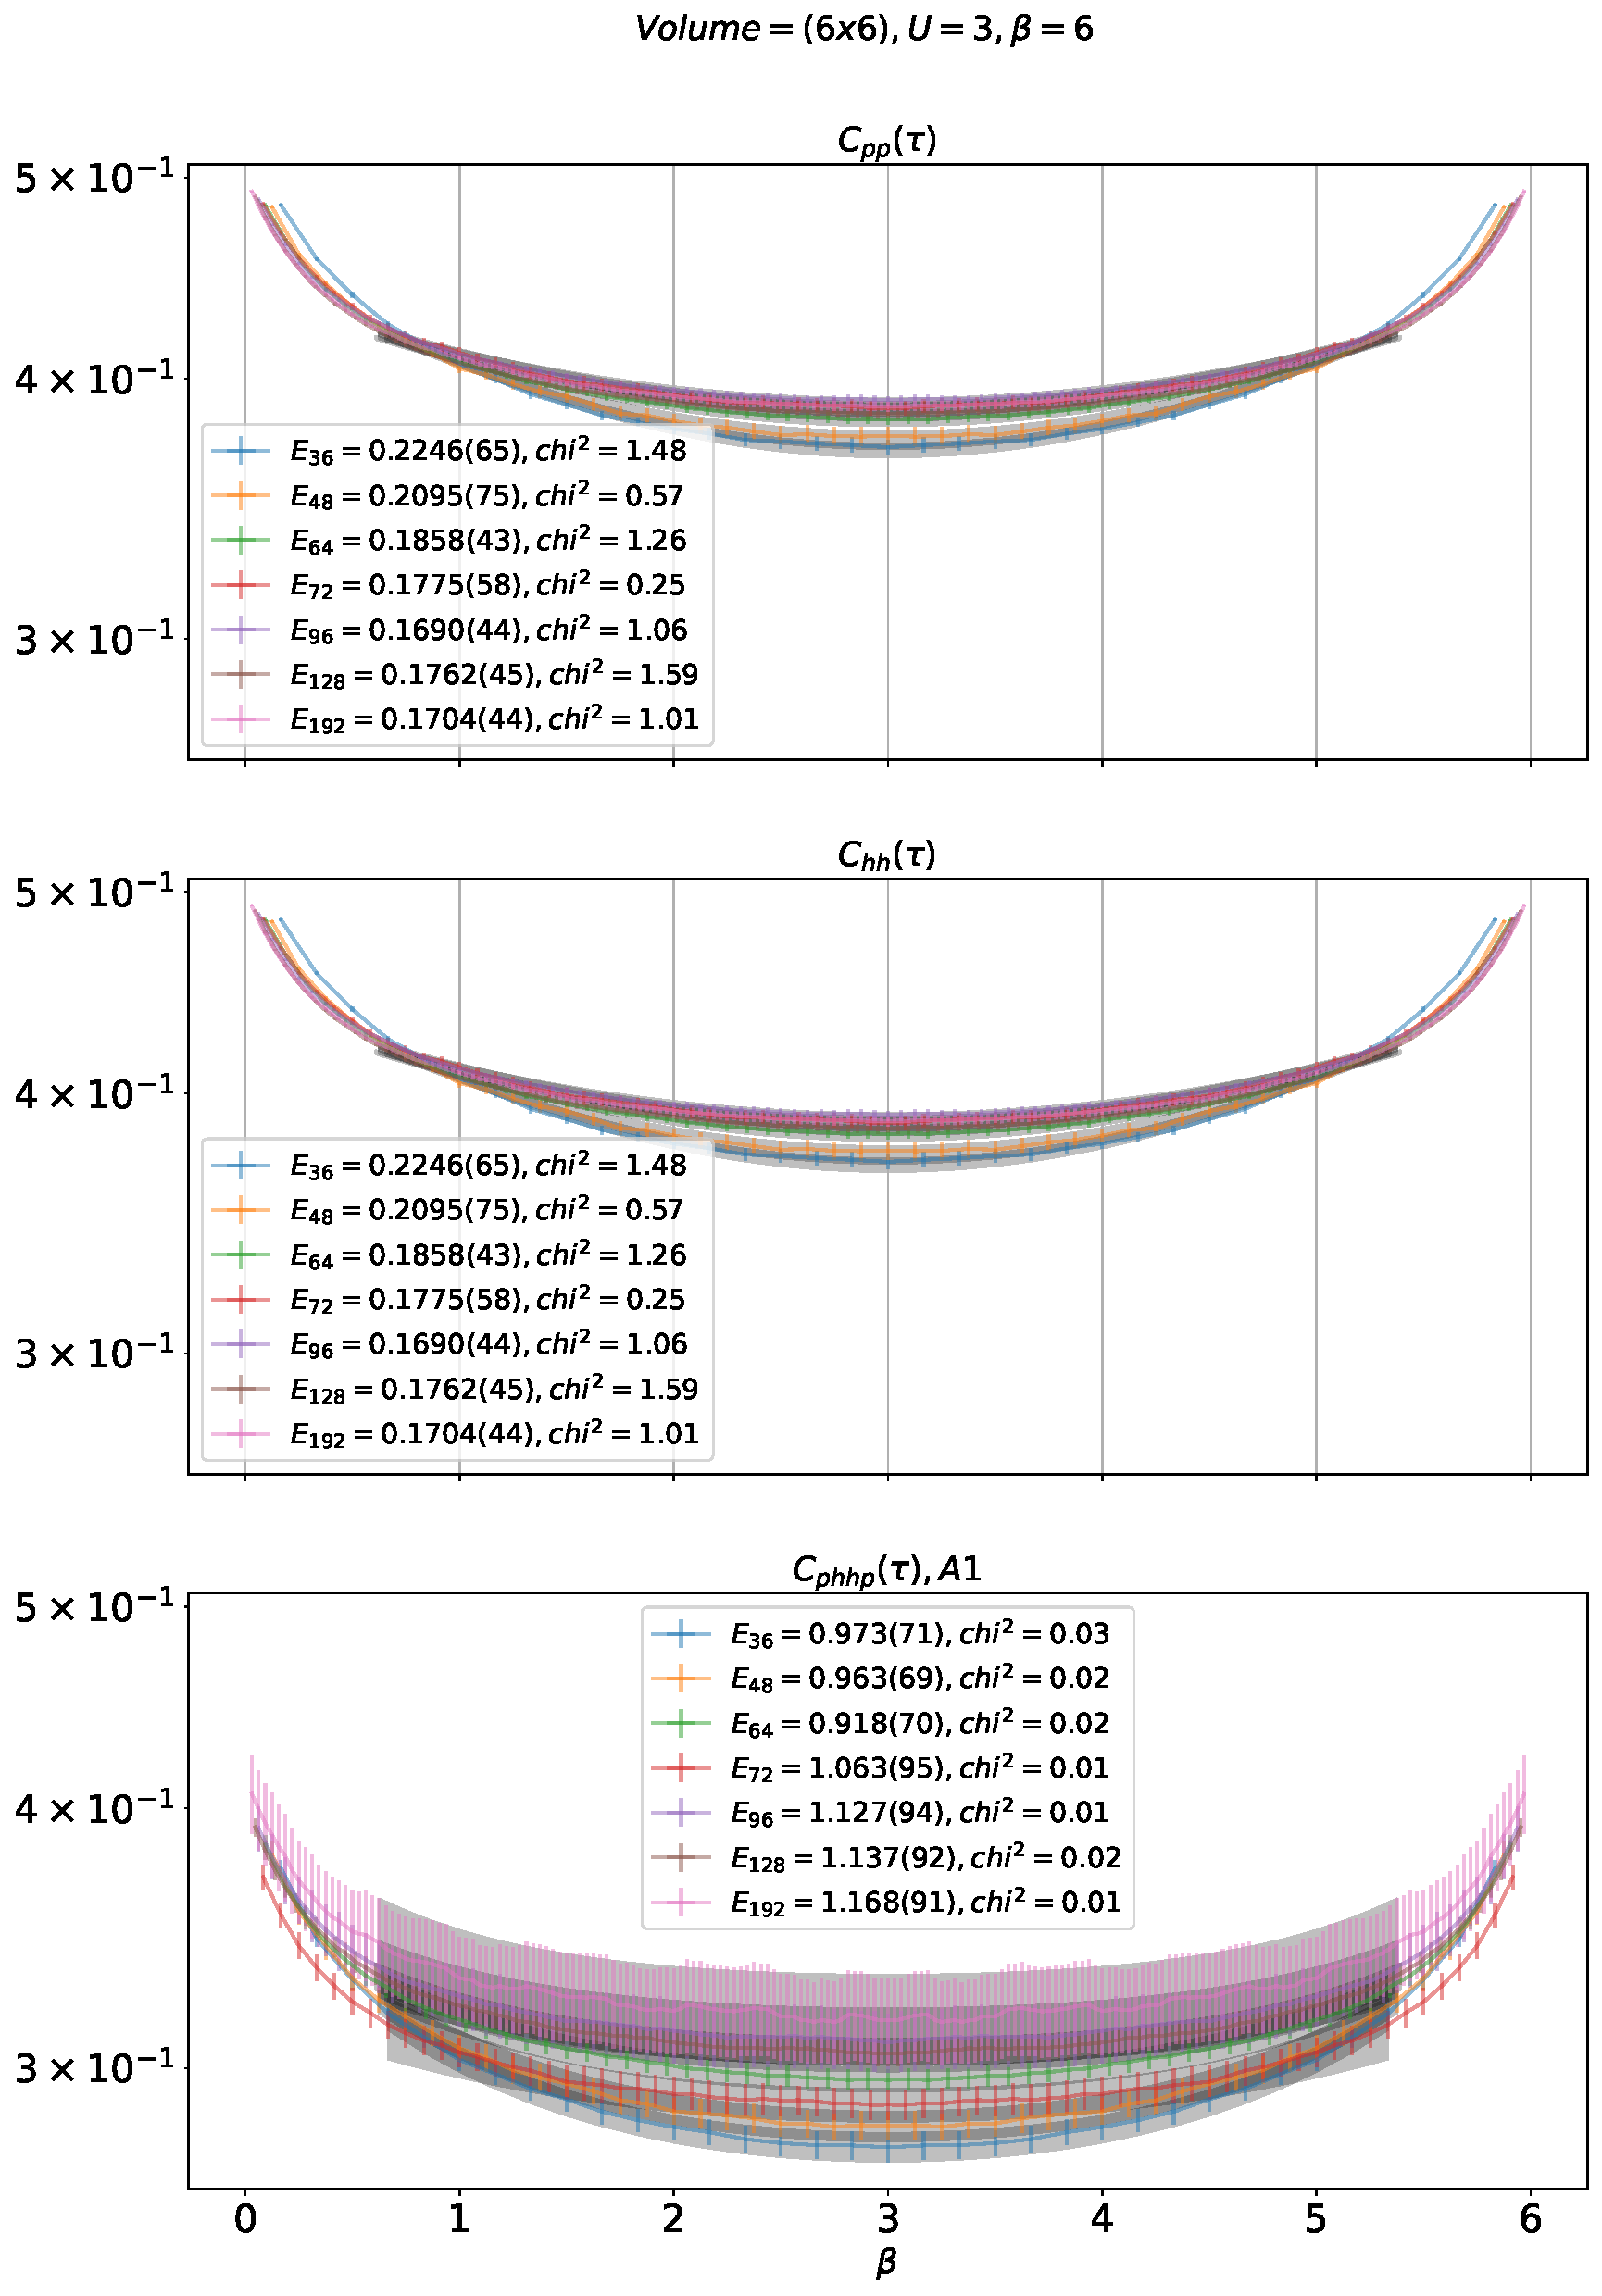
\includegraphics[width=\linewidth]{phhp-0-A1_6x6_U3.0_B6.0.pdf}
  \end{subfigure}%
  \begin{subfigure}{.5\textwidth}
    \centering
    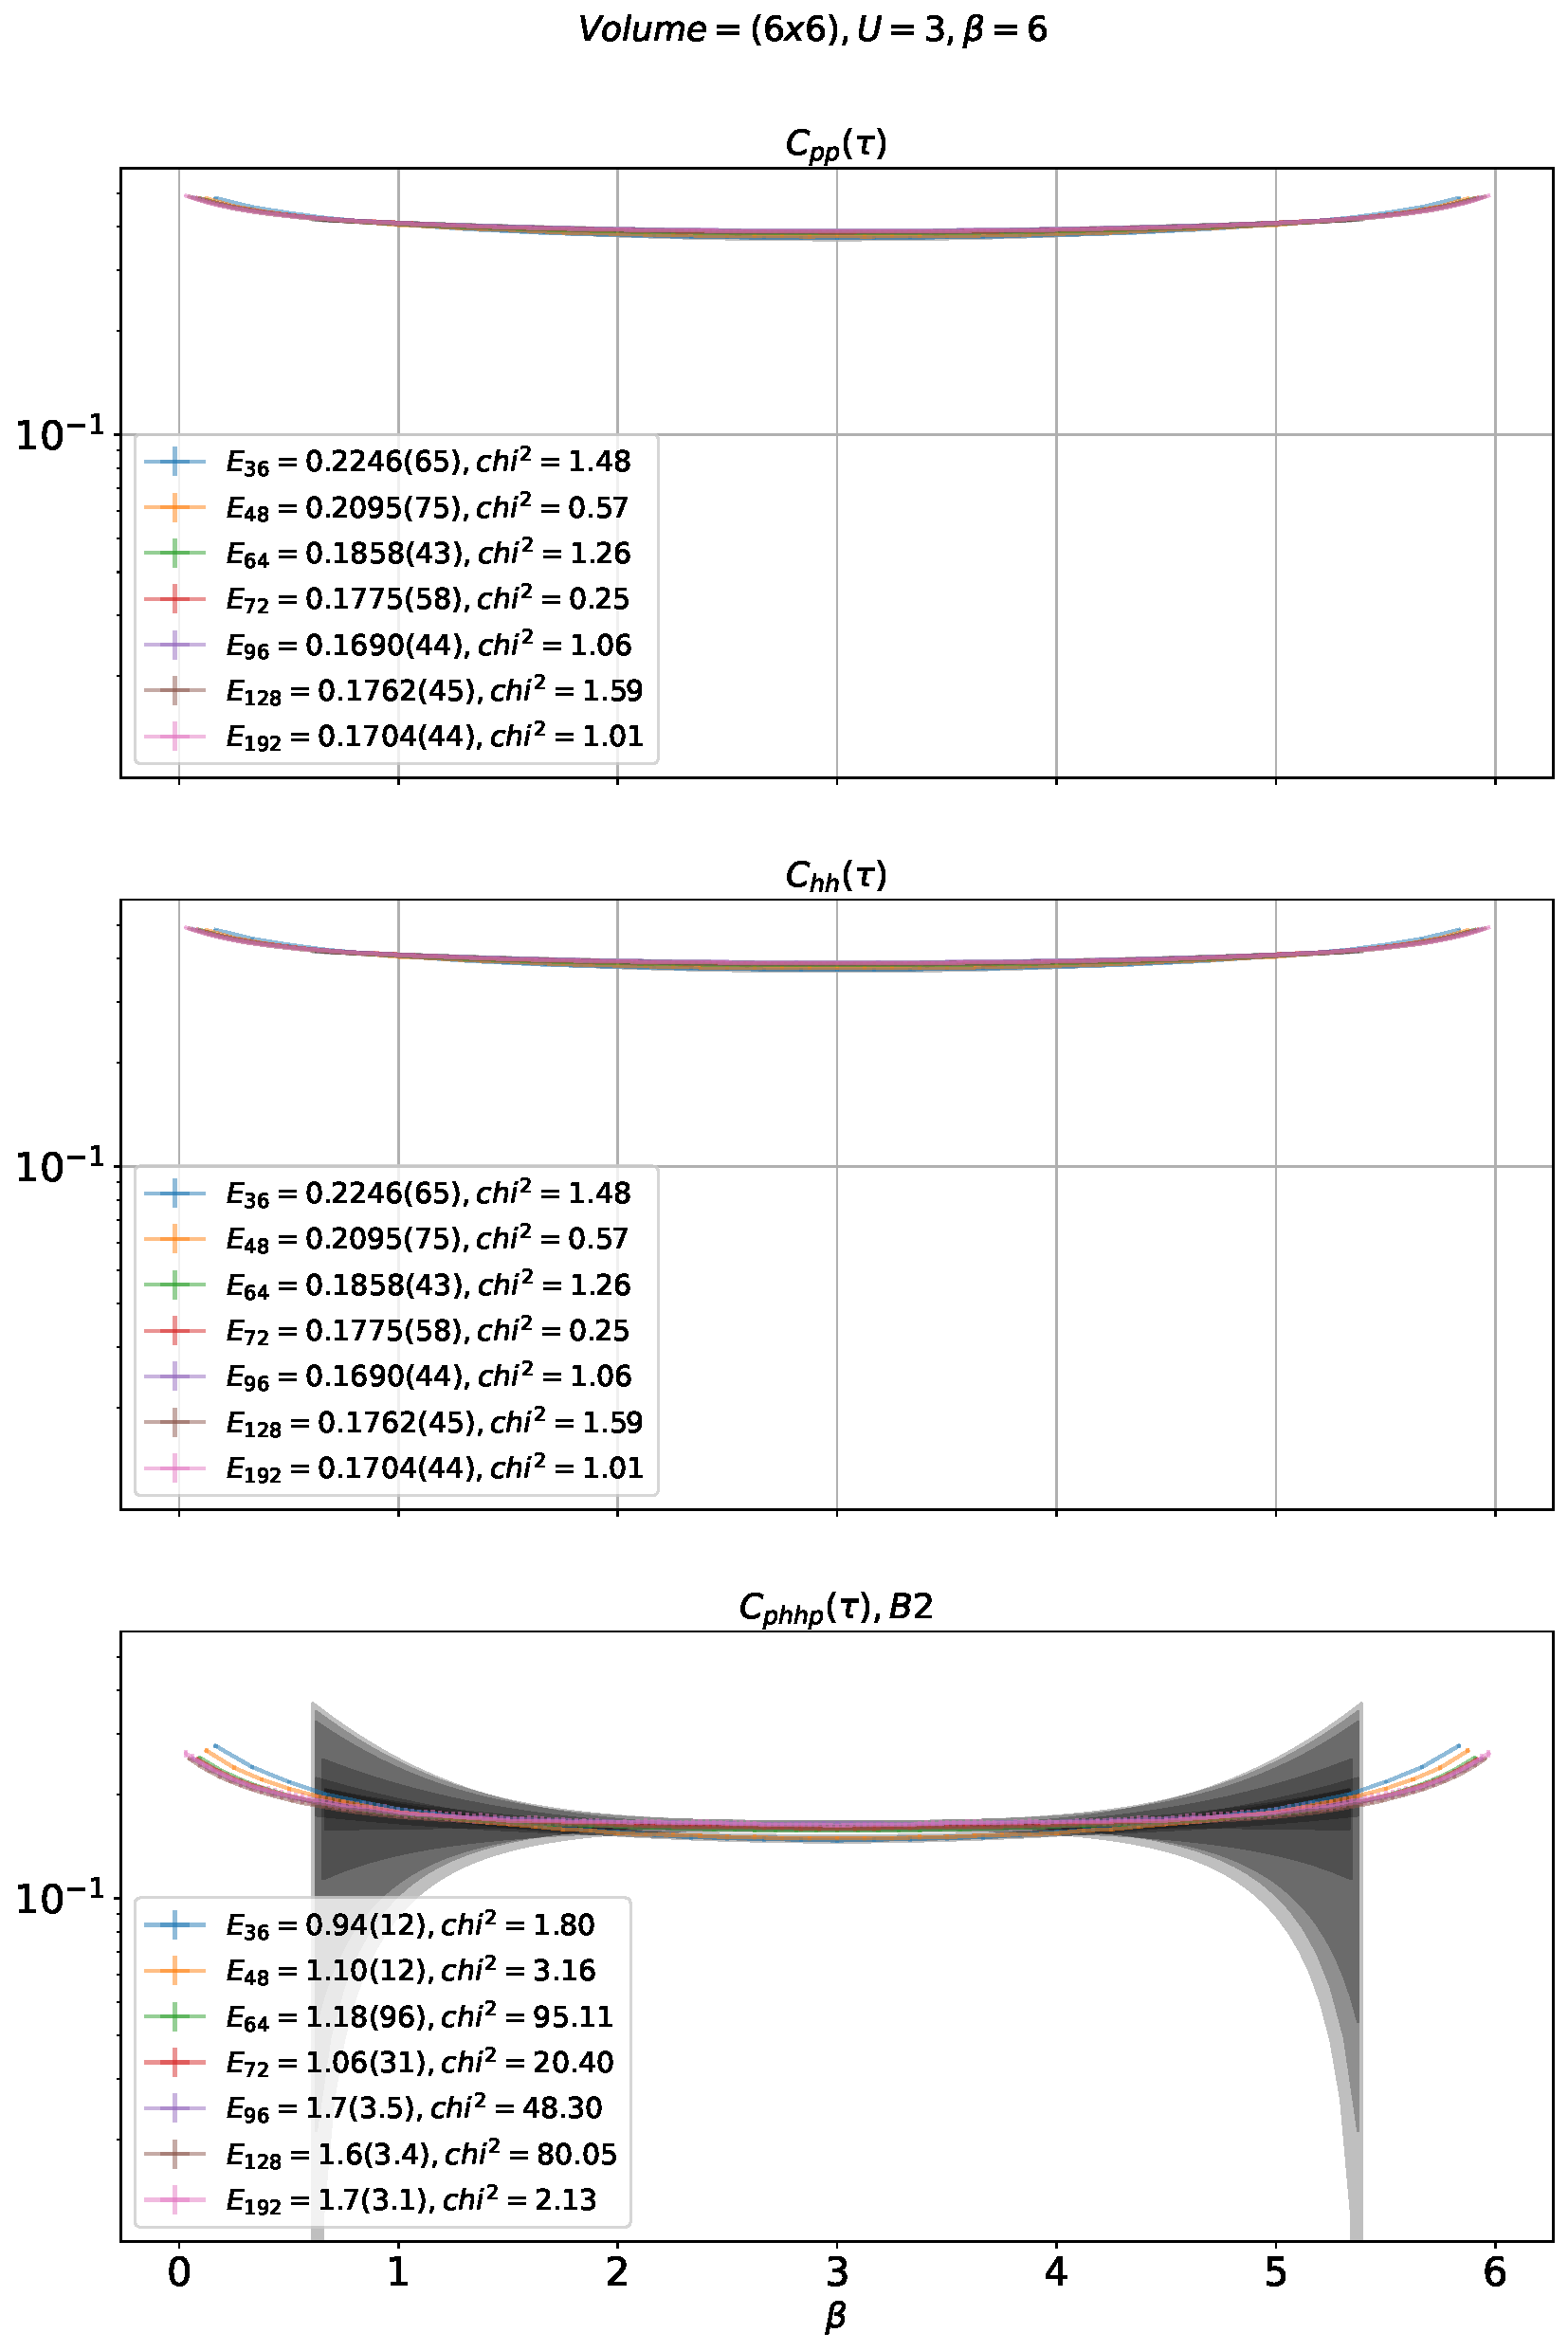
\includegraphics[width=\linewidth]{phhp-0-B2_6x6_U3.0_B6.0.pdf}
  \end{subfigure}
  \begin{subfigure}{.5\textwidth}
      \centering
      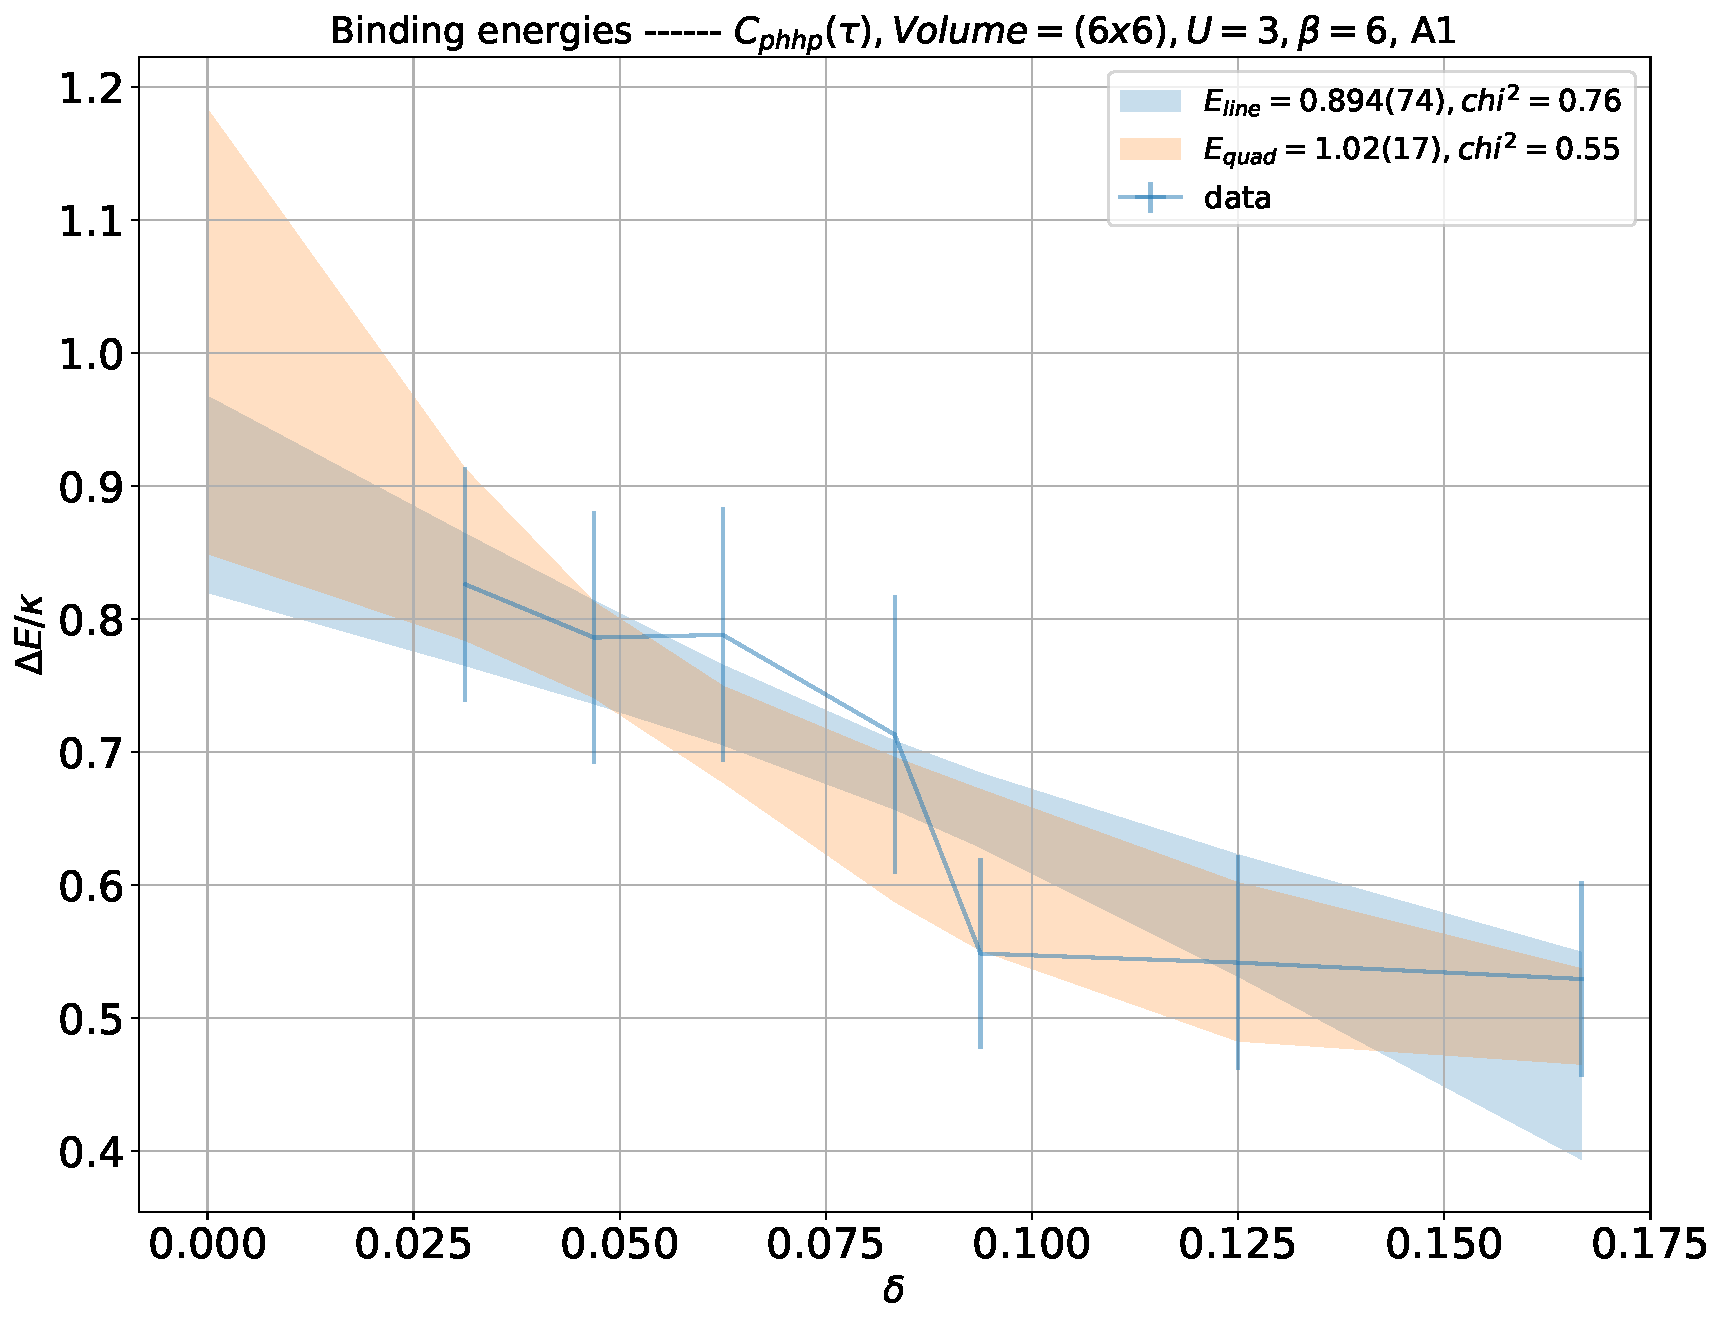
\includegraphics[width=\linewidth]{phhp-0-A1_6x6_U3.0_B6.0_cont.pdf}
  \end{subfigure}
  \begin{subfigure}{.5\textwidth}
      \centering
      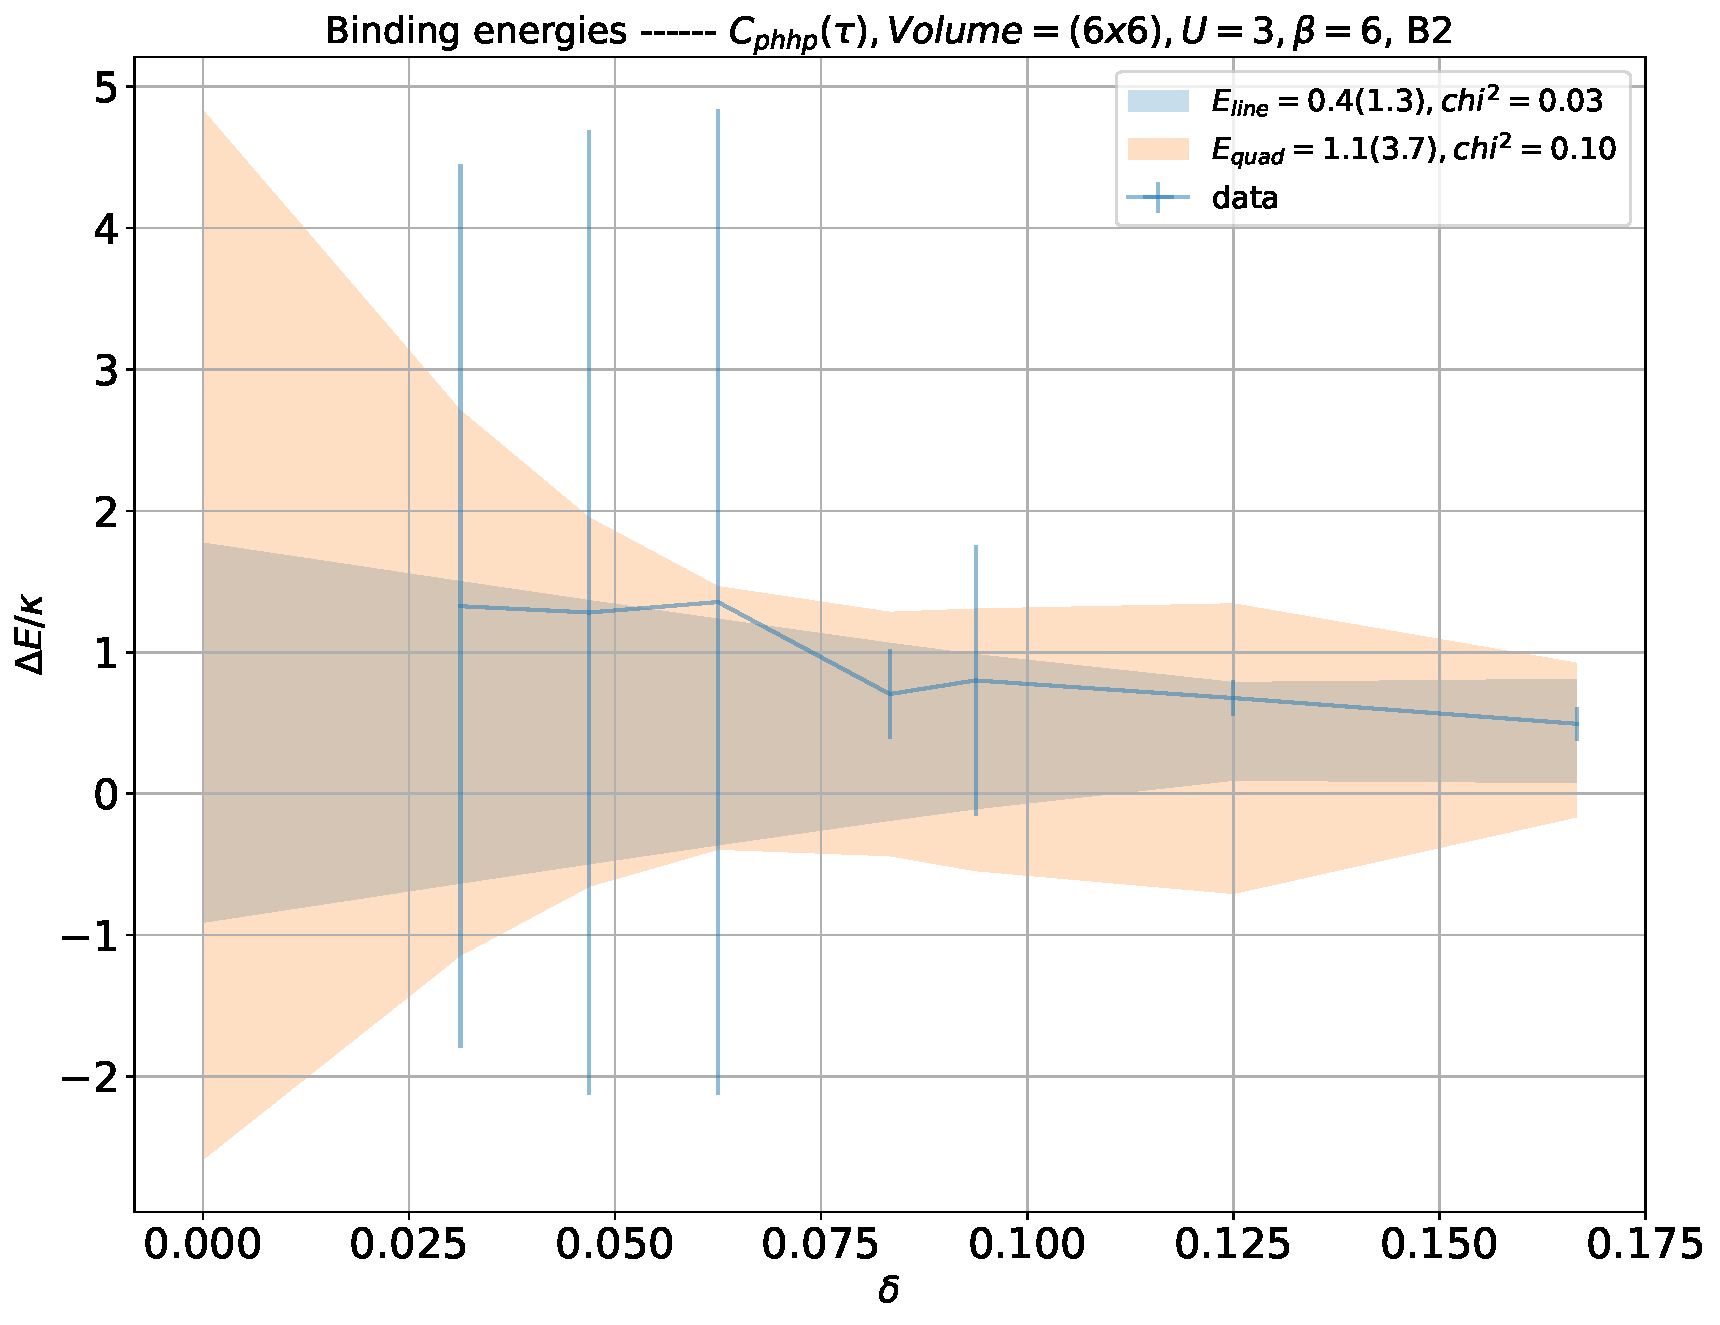
\includegraphics[width=\linewidth]{phhp-0-B2_6x6_U3.0_B6.0_cont.pdf}
  \end{subfigure}
  \caption{Binding energy extraction of the particle-hole pair at both irreducible representations, where we fit one- and two-body correlators for every $N_t$. This is followed by fitting a linear and a quadratic functions to the $\Delta E_{N_t}$ in order to extrapolate to the continuum limit ($N_t\to\infty$).}
  \label{fig:fig1}
\end{figure}

\begin{figure}
  \begin{subfigure}{.5\textwidth}
    \centering
    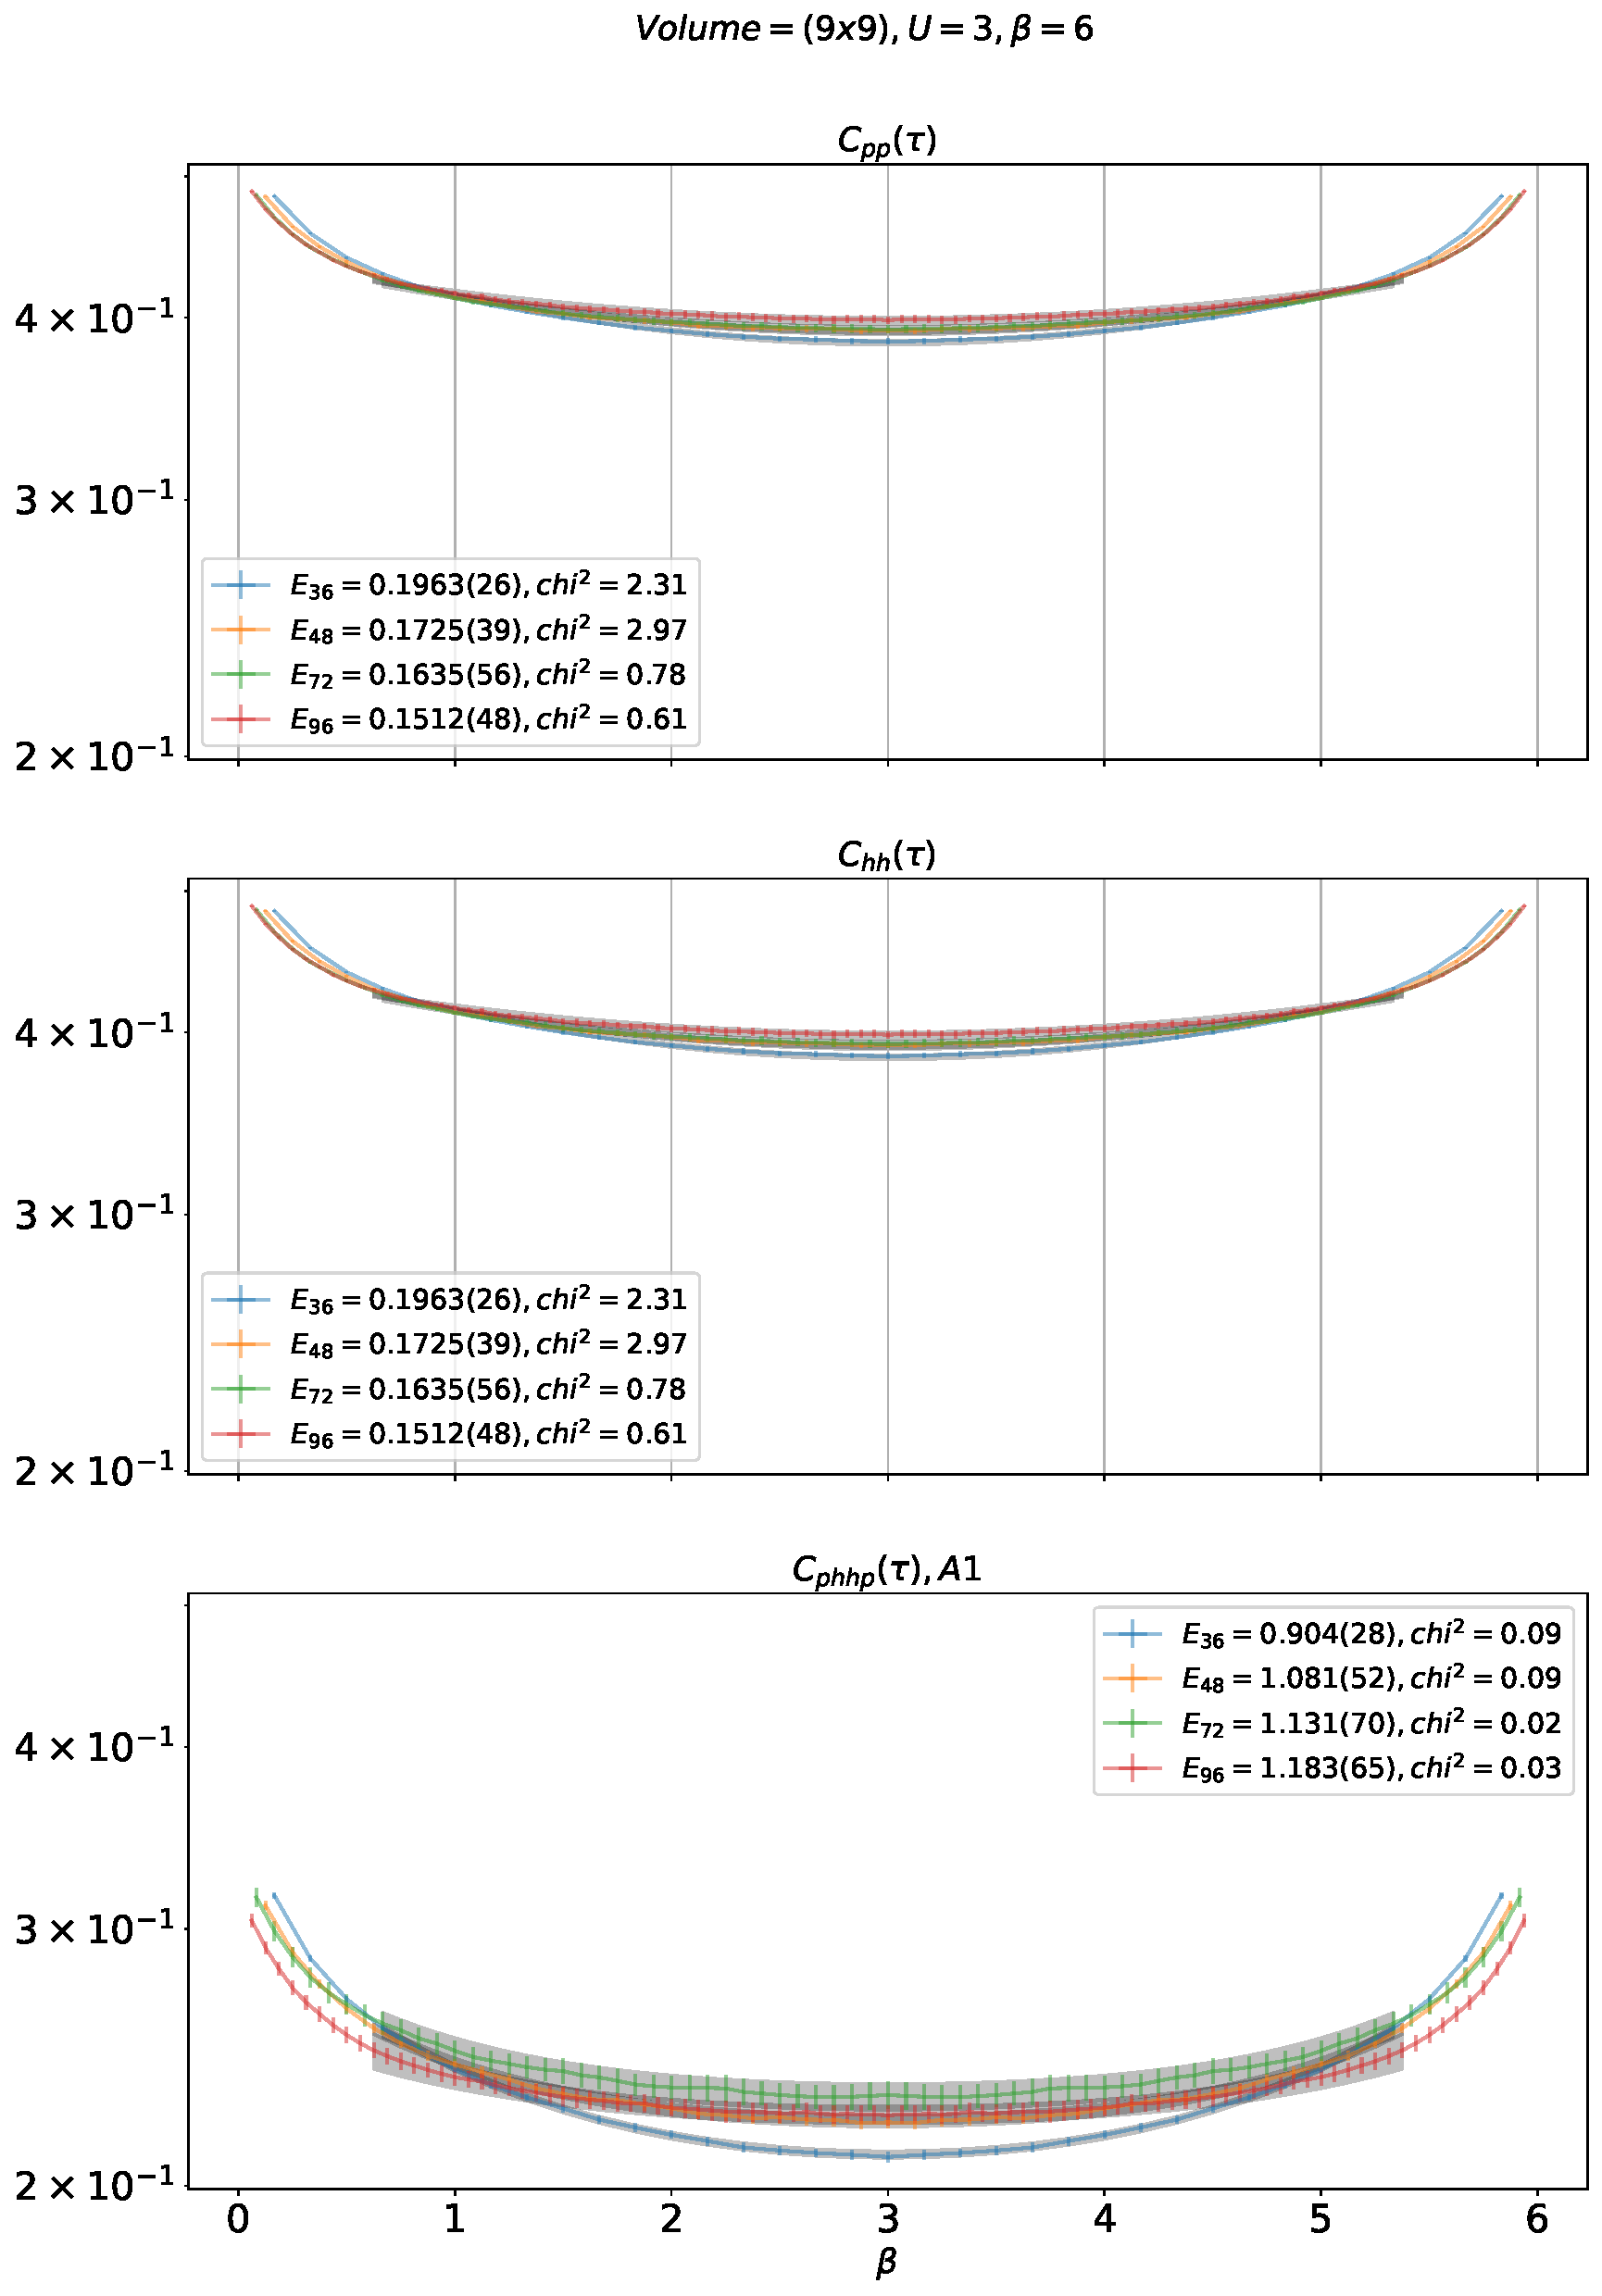
\includegraphics[width=\linewidth]{phhp-0-A1_9x9_U3_B6.pdf}
  \end{subfigure}%
  \begin{subfigure}{.5\textwidth}
    \centering
    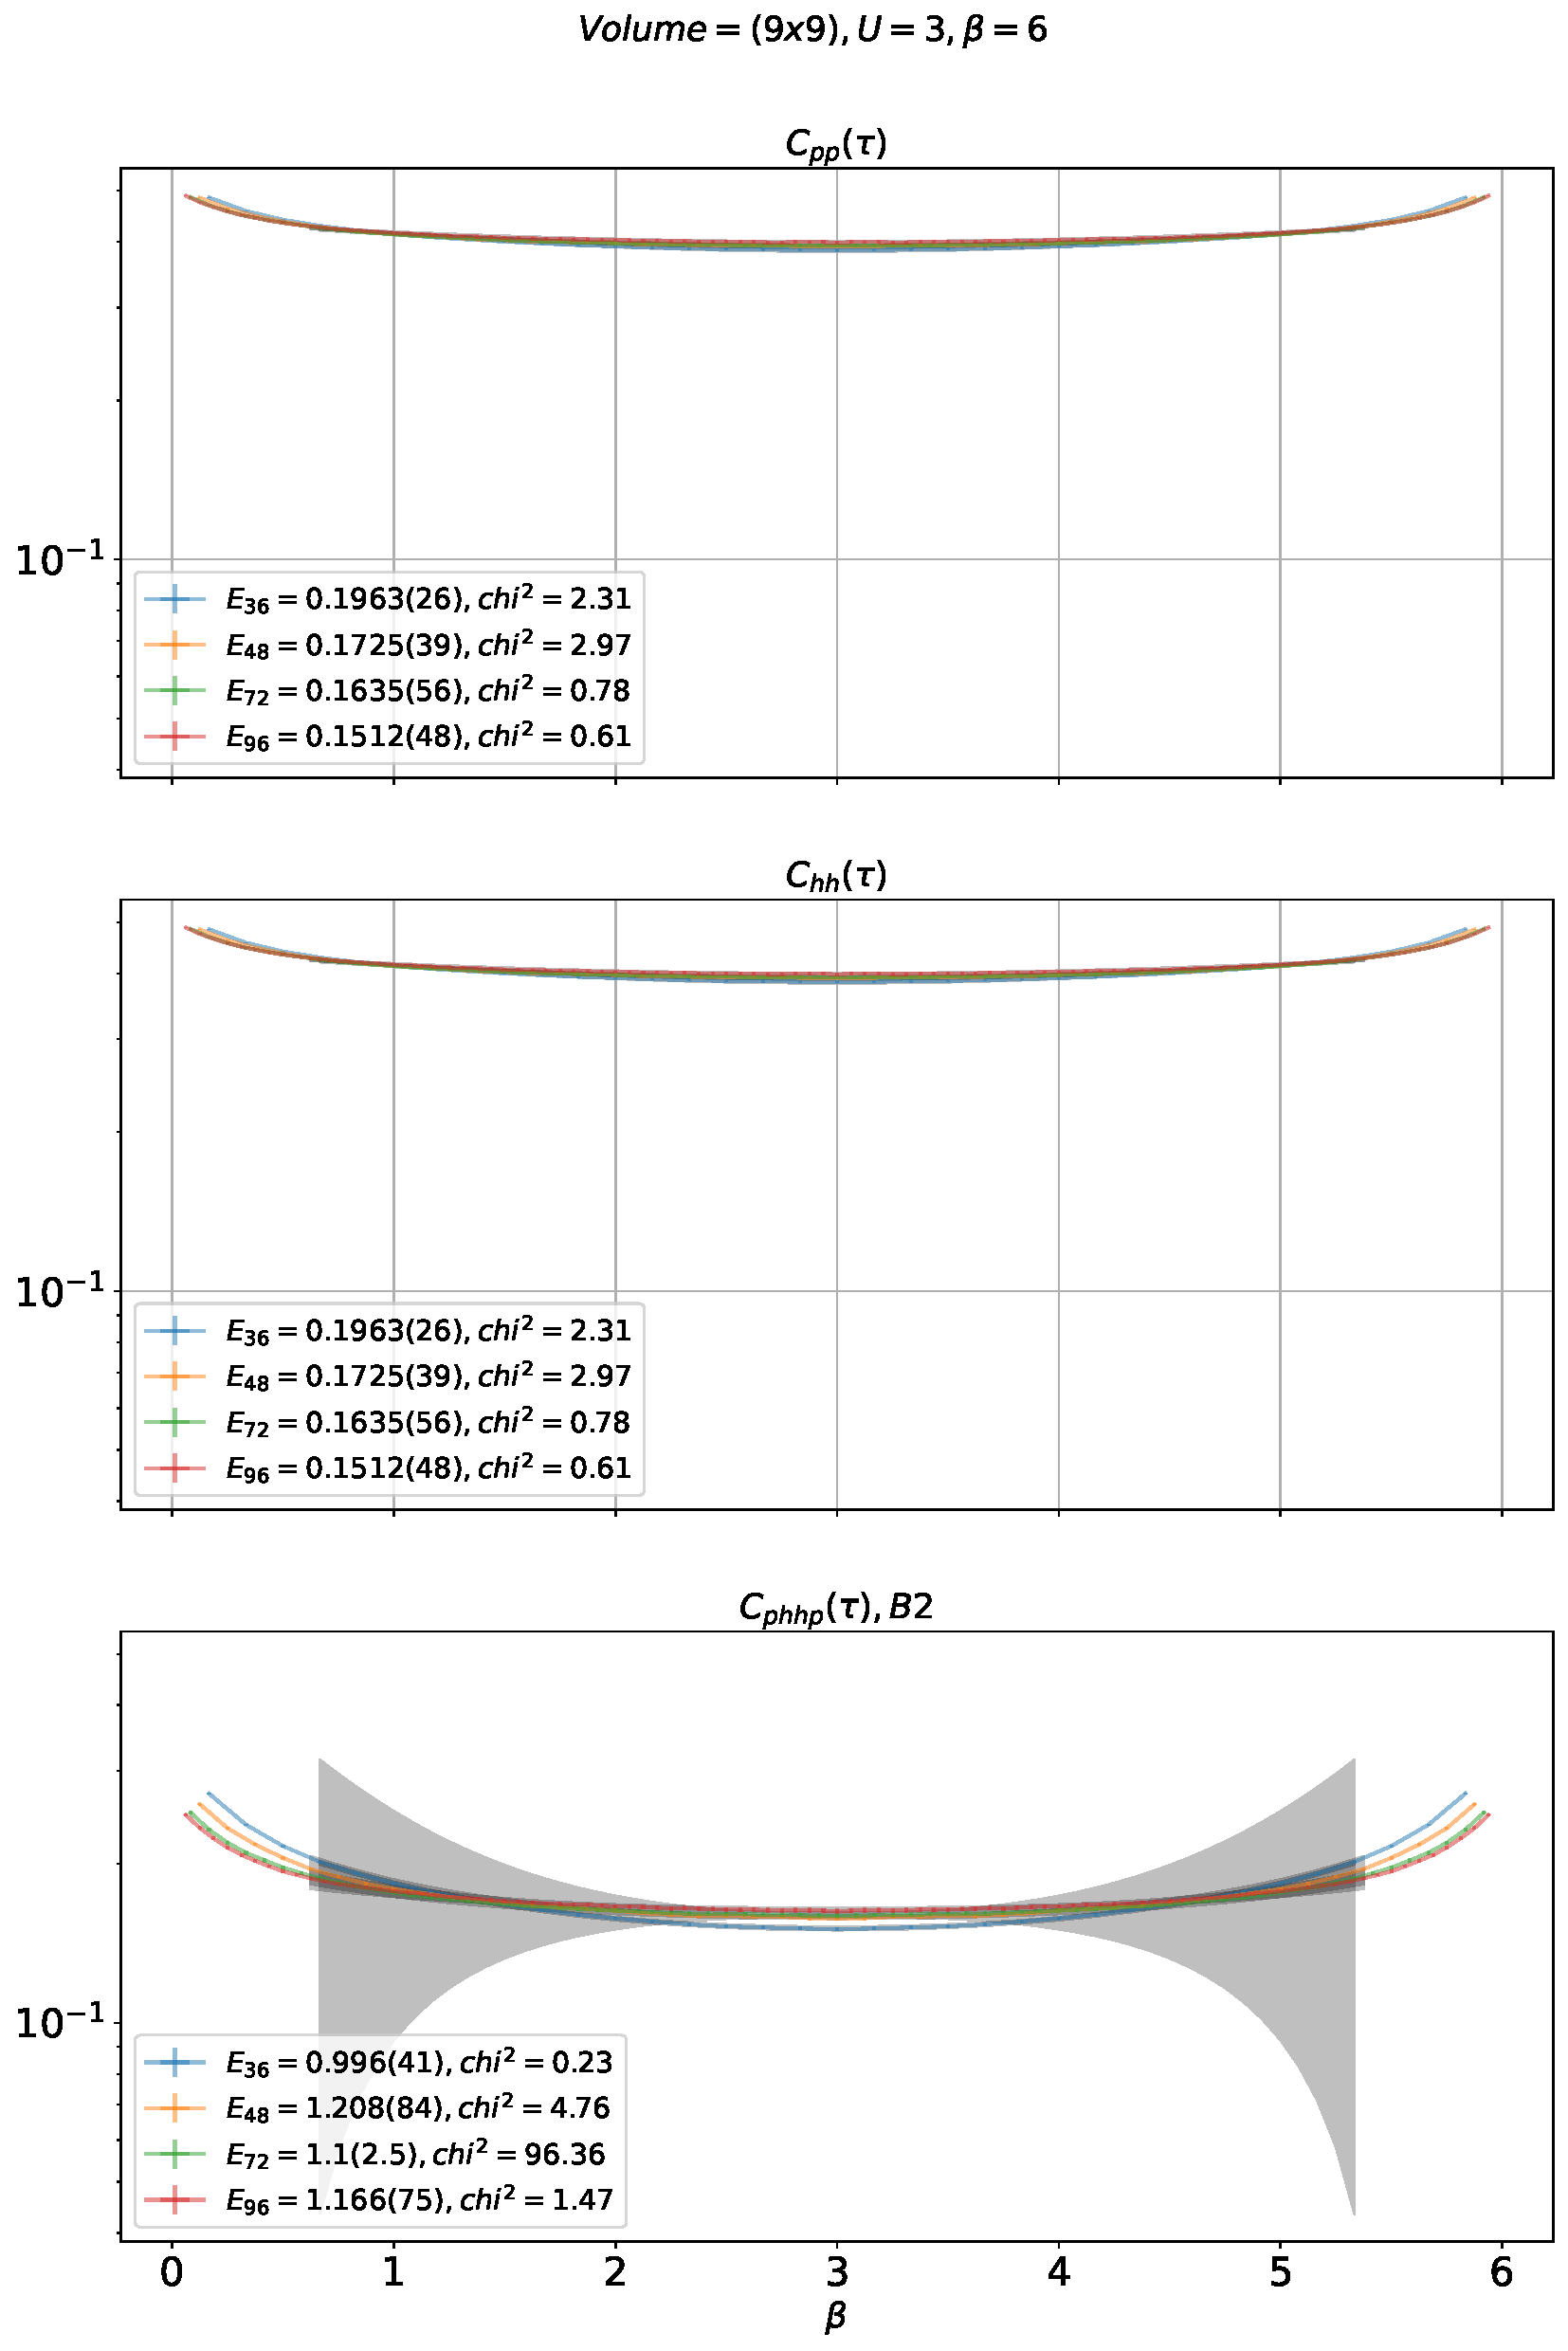
\includegraphics[width=\linewidth]{phhp-0-B2_9x9_U3_B6.pdf}
  \end{subfigure}
  \begin{subfigure}{.5\textwidth}
      \centering
      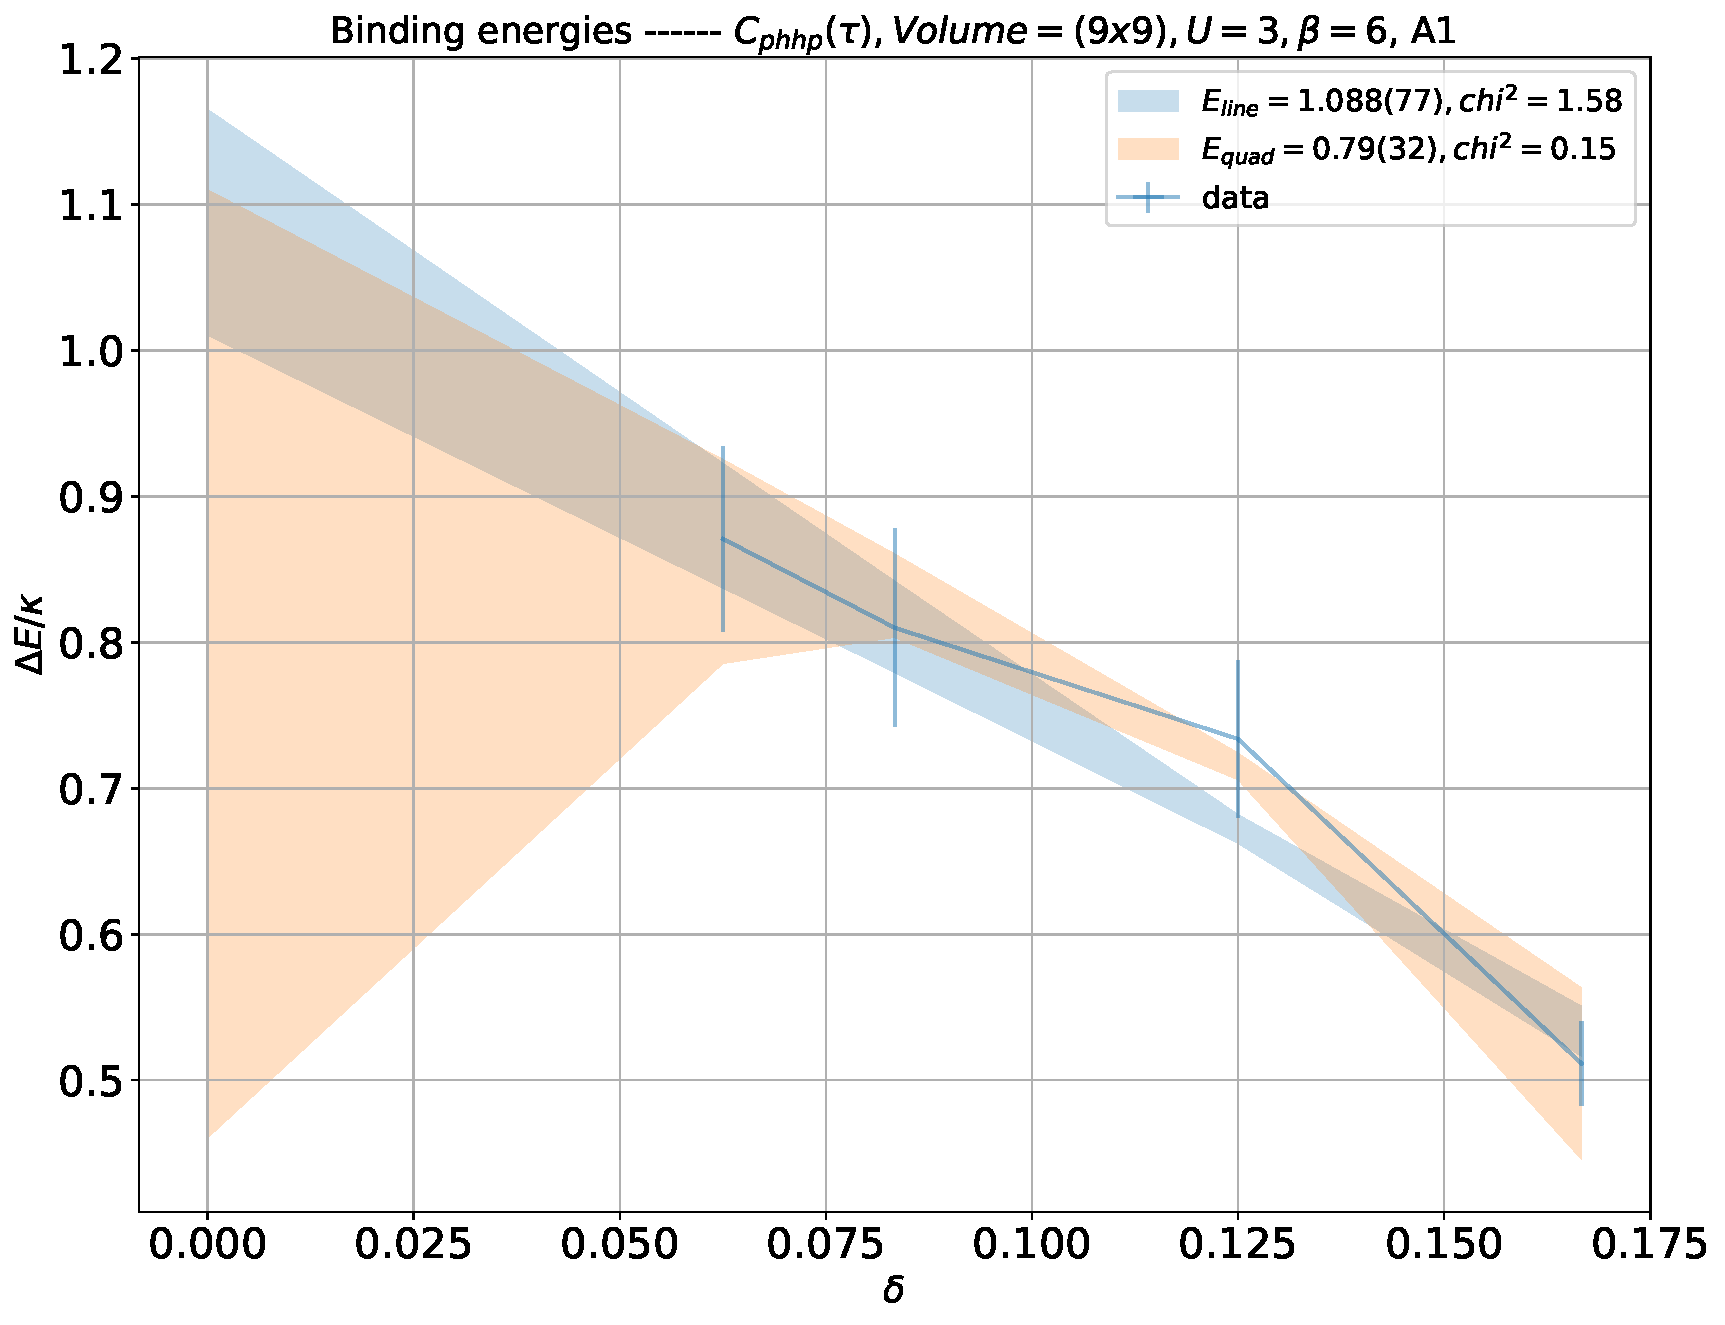
\includegraphics[width=\linewidth]{phhp-0-A1_9x9_U3_B6_cont.pdf}
  \end{subfigure}
  \begin{subfigure}{.5\textwidth}
      \centering
      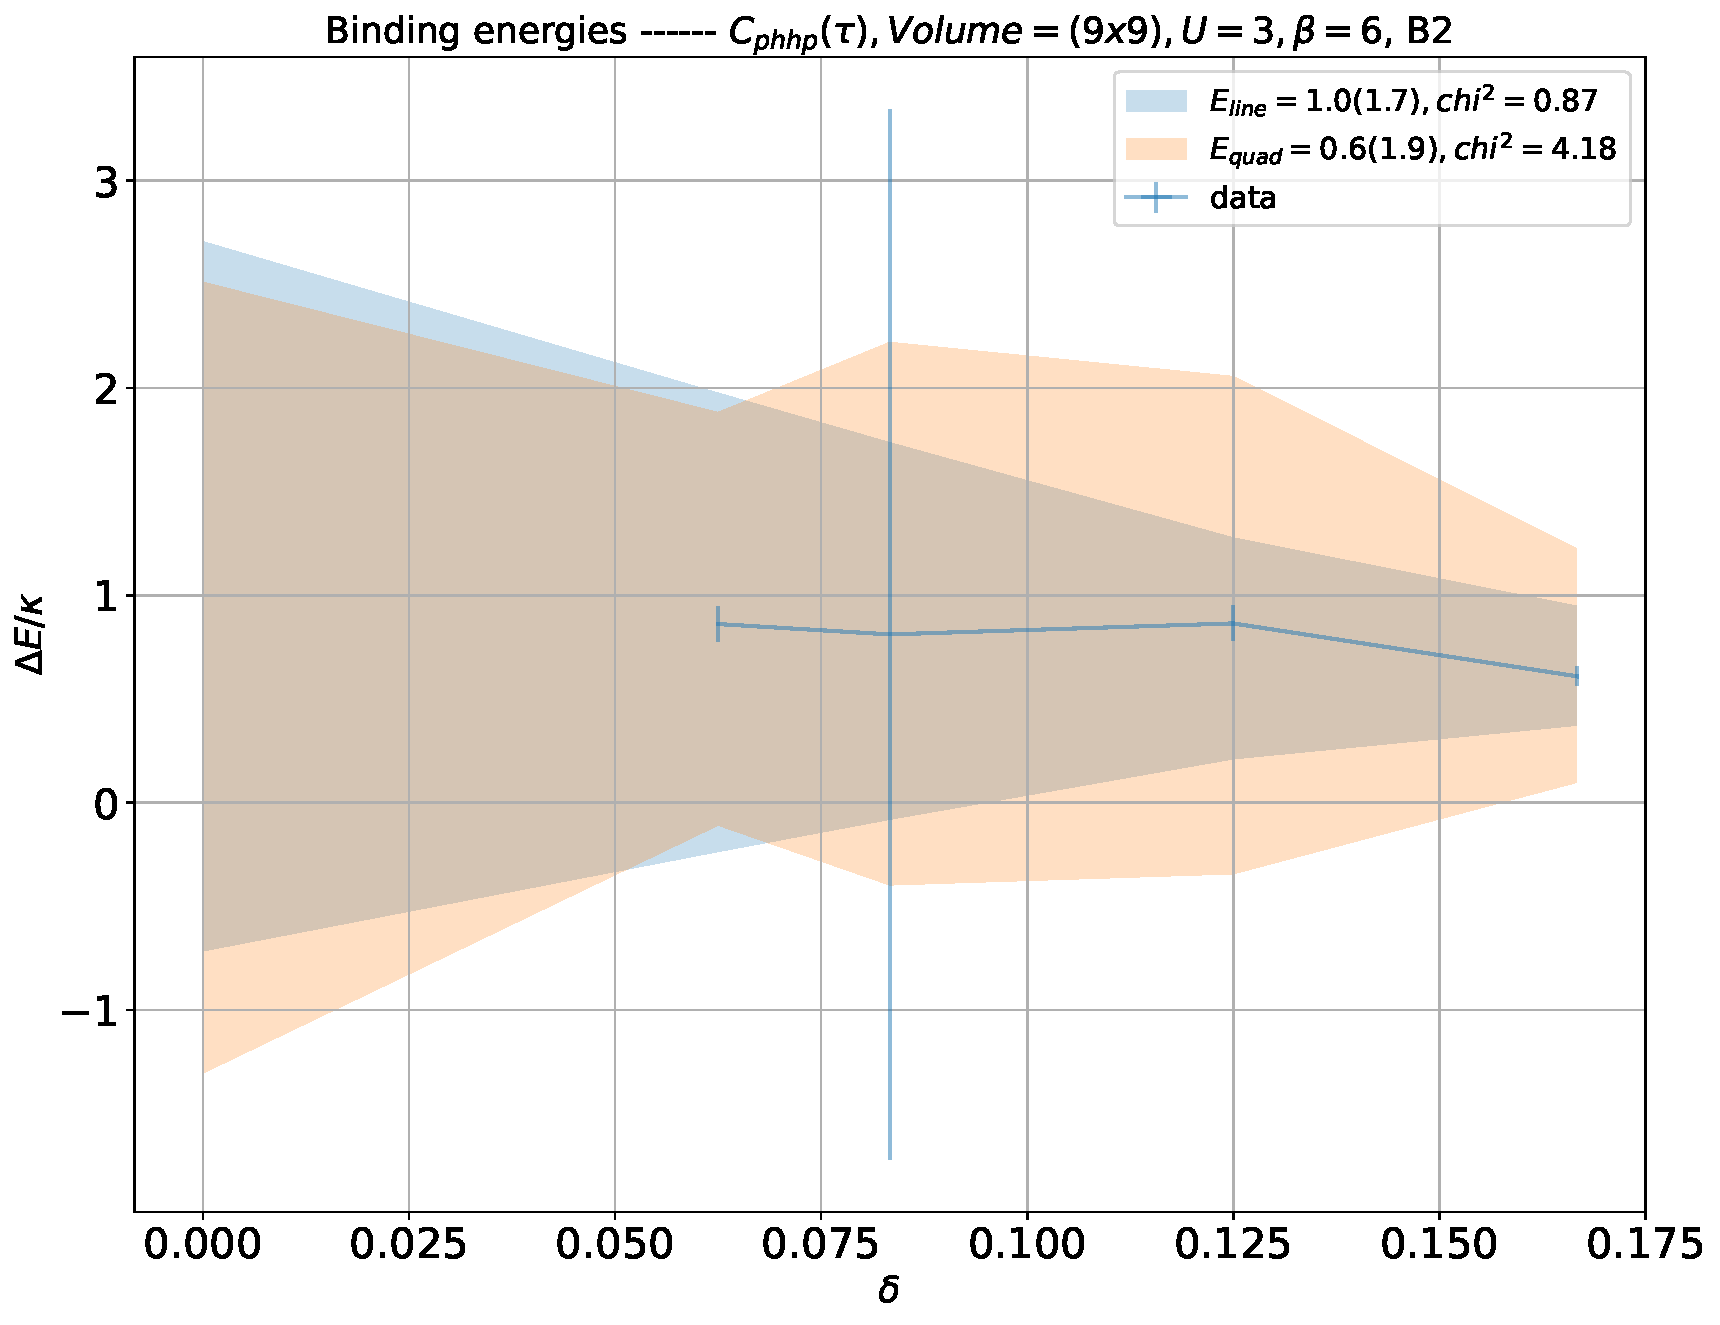
\includegraphics[width=\linewidth]{phhp-0-B2_9x9_U3_B6_cont.pdf}
  \end{subfigure}
  \caption{Binding energy extraction of the particle-hole pair at both irreducible representations, where we fit one- and two-body correlators for every $N_t$. This is followed by fitting a linear and a quadratic functions to the $\Delta E_{N_t}$ in order to extrapolate to the continuum limit ($N_t\to\infty$).}
  \label{fig:fig2}
\end{figure}

\begin{figure}
  \begin{subfigure}{.5\textwidth}
    \centering
    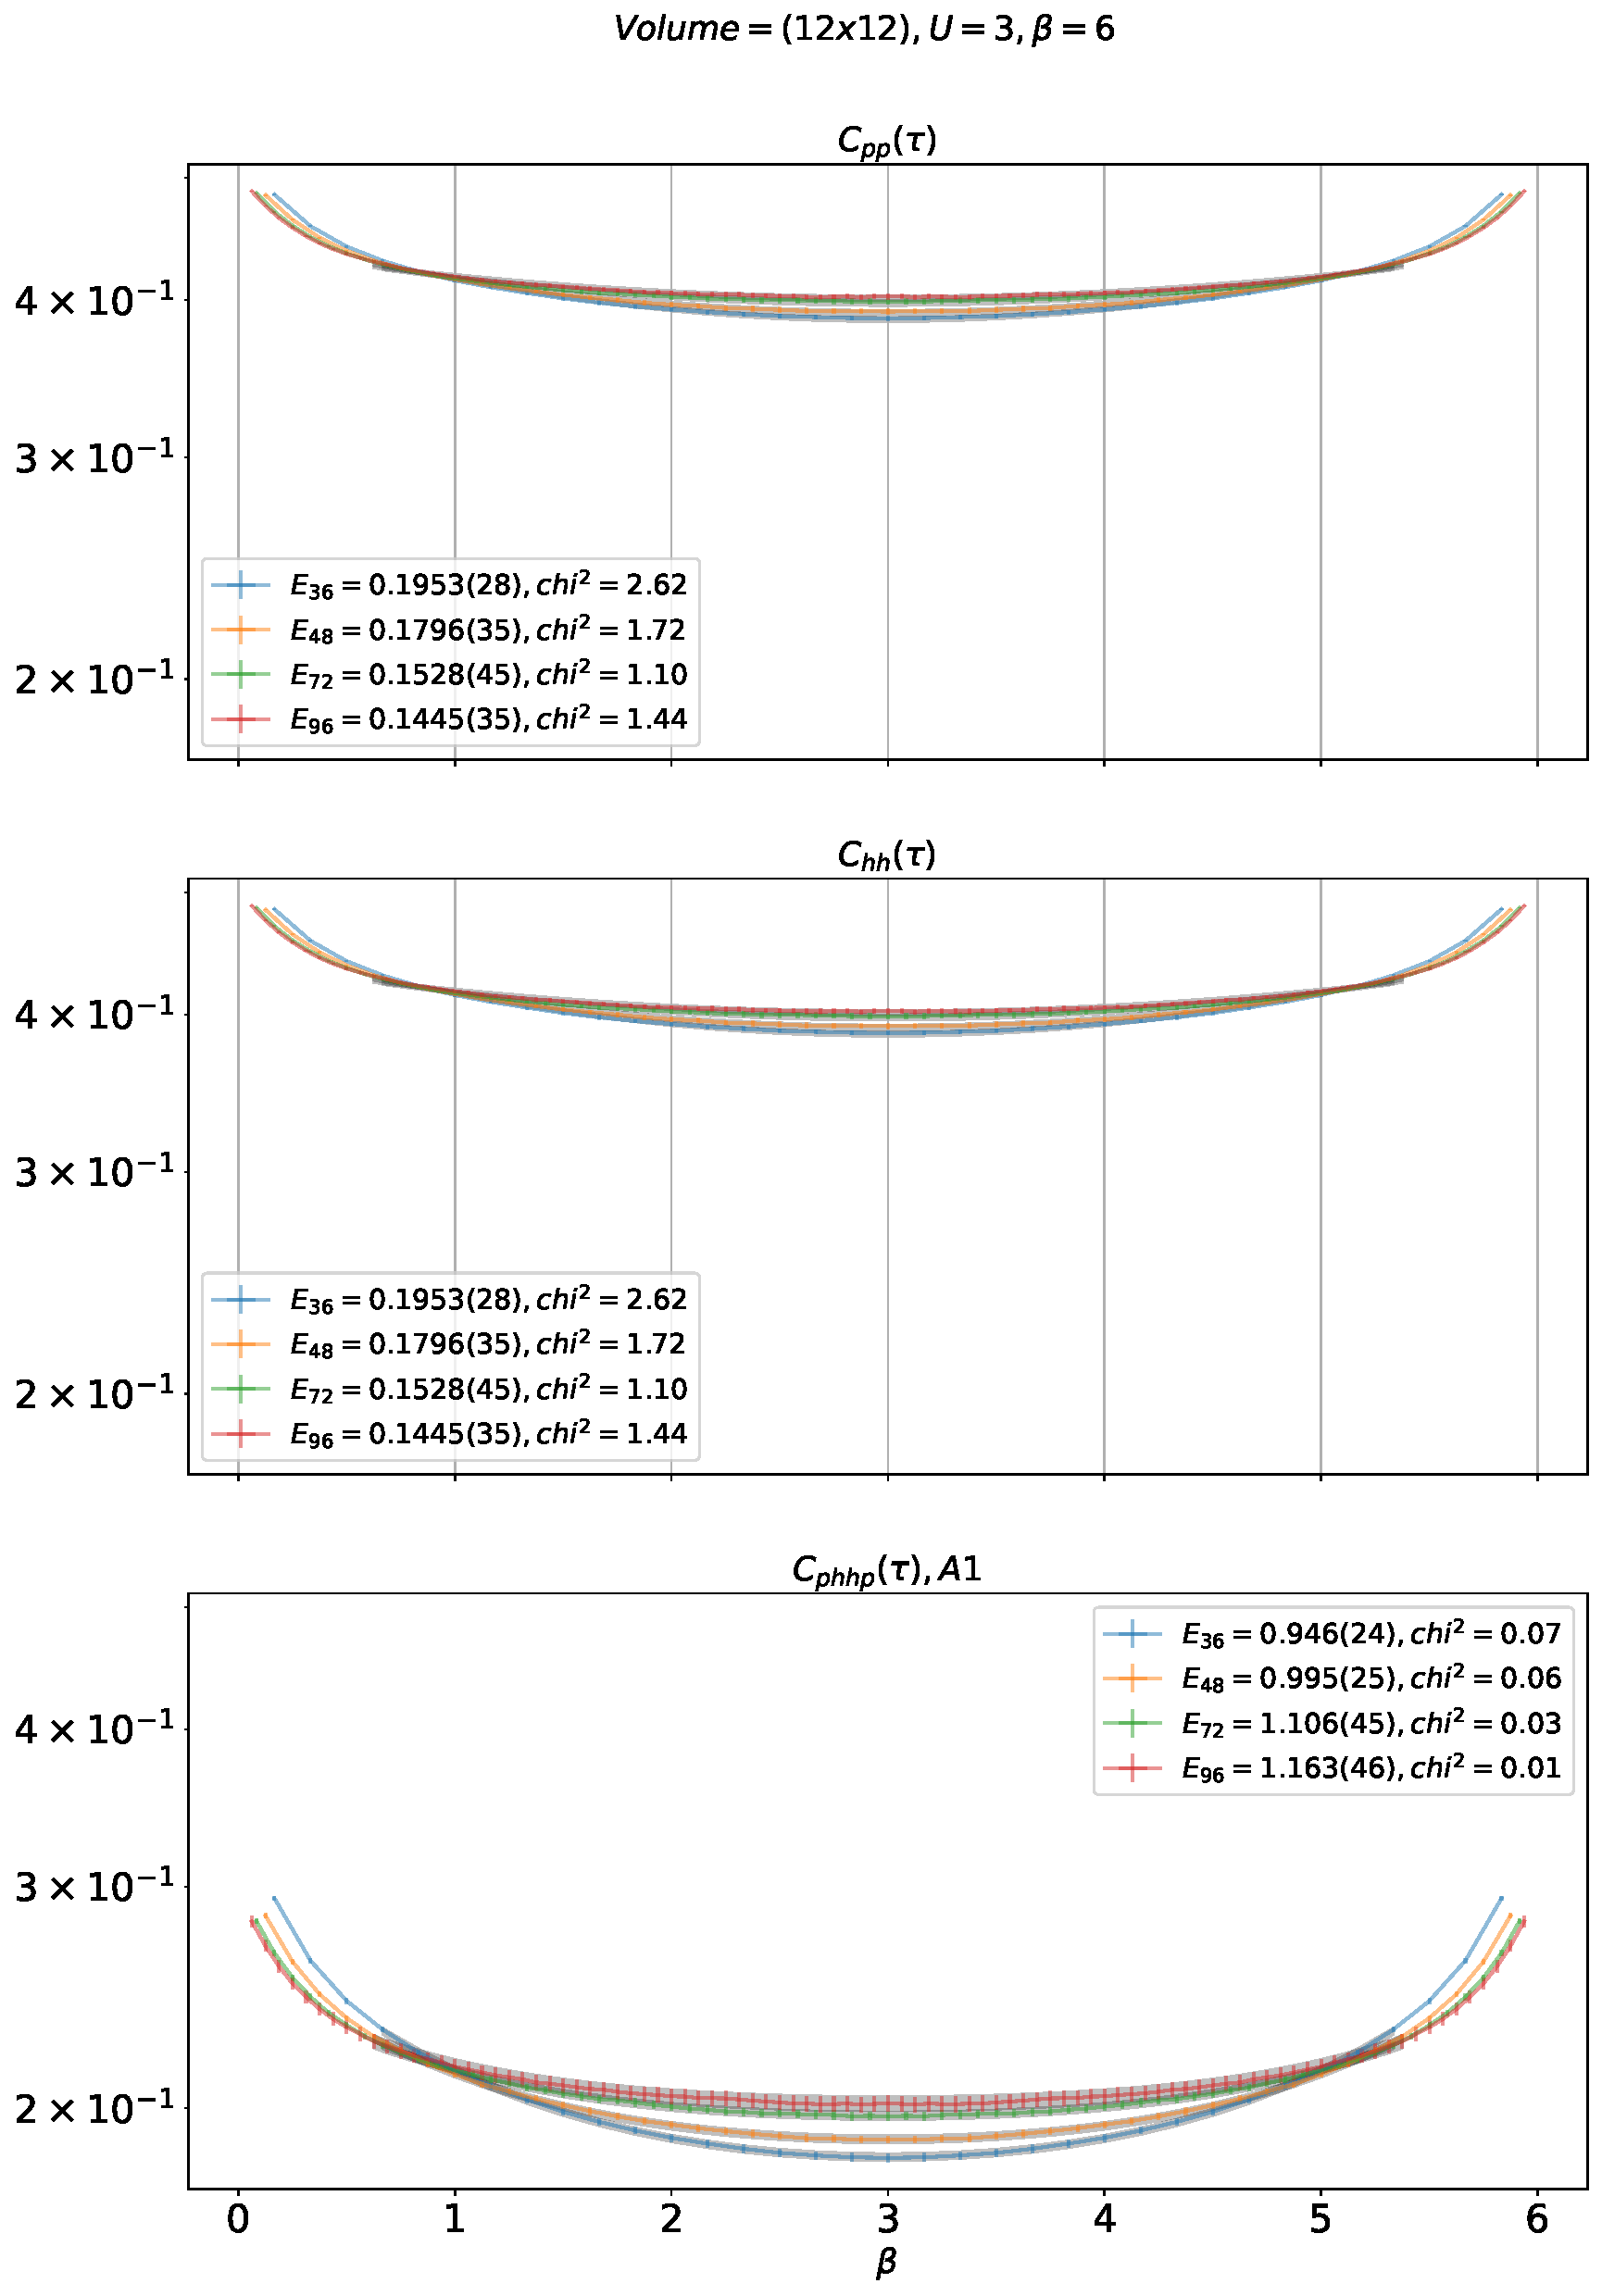
\includegraphics[width=\linewidth]{phhp-0-A1_12x12_U3_B6.pdf}
  \end{subfigure}%
  \begin{subfigure}{.5\textwidth}
    \centering
    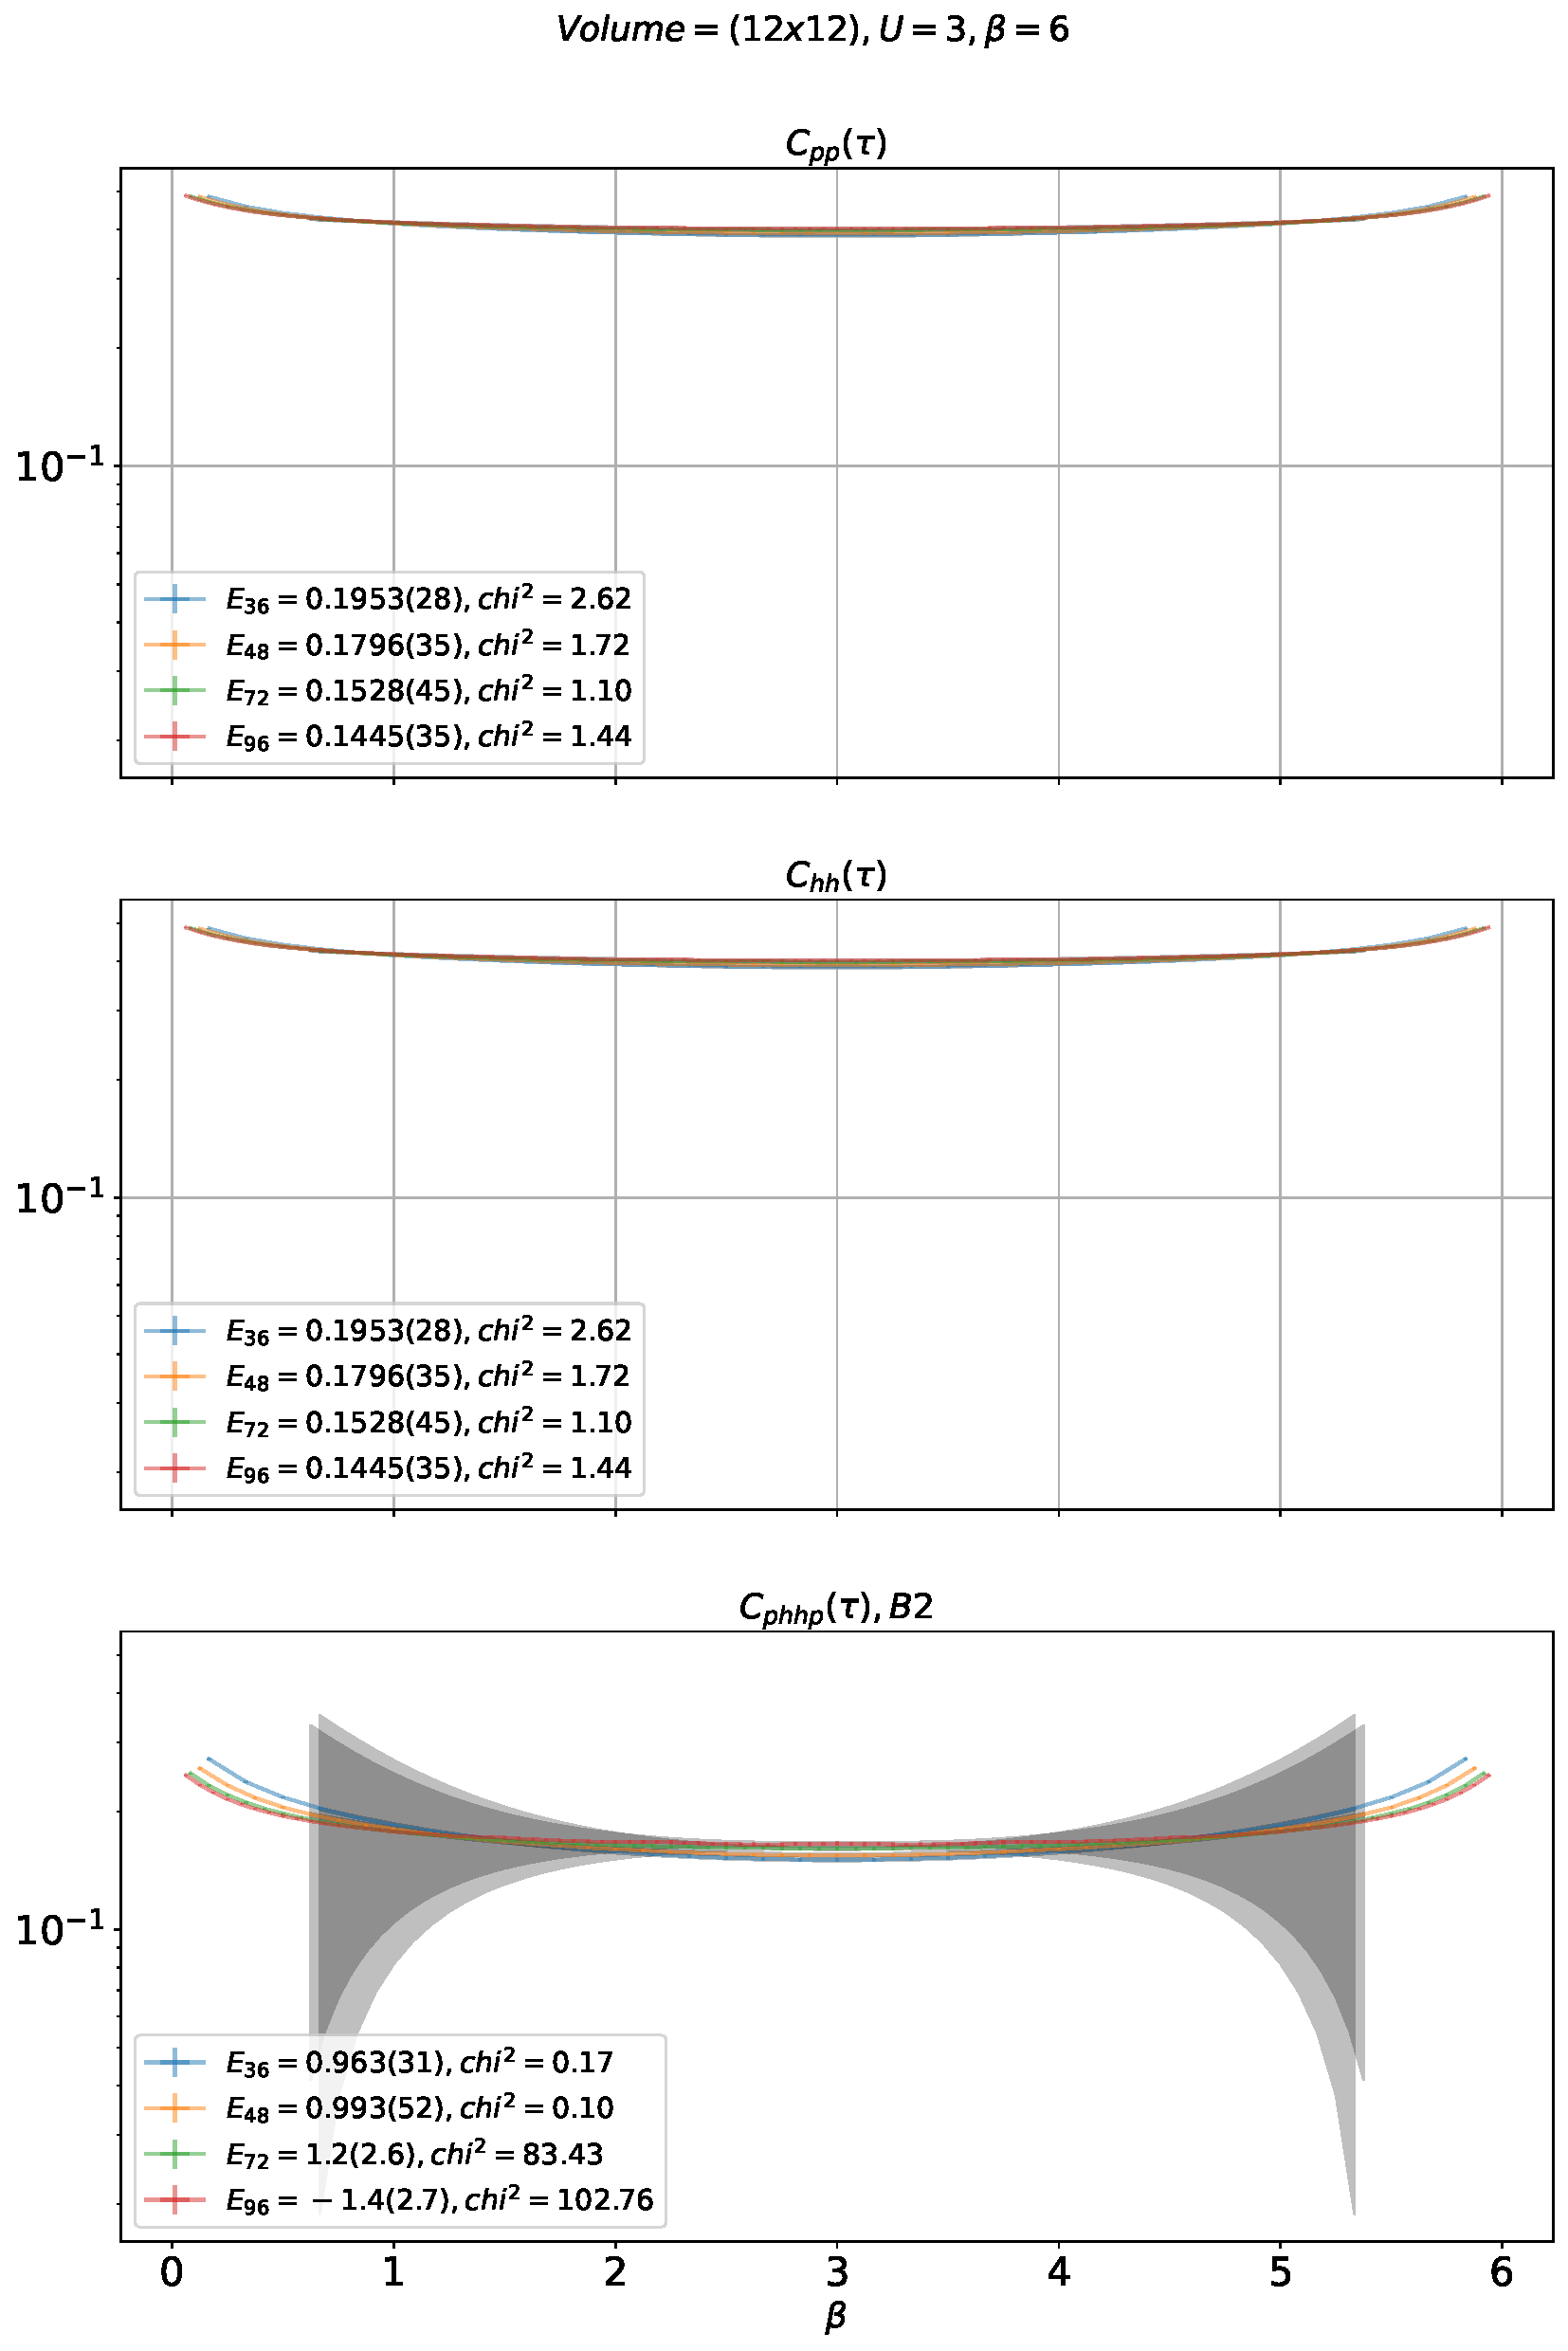
\includegraphics[width=\linewidth]{phhp-0-B2_12x12_U3_B6.pdf}
  \end{subfigure}
  \begin{subfigure}{.5\textwidth}
      \centering
      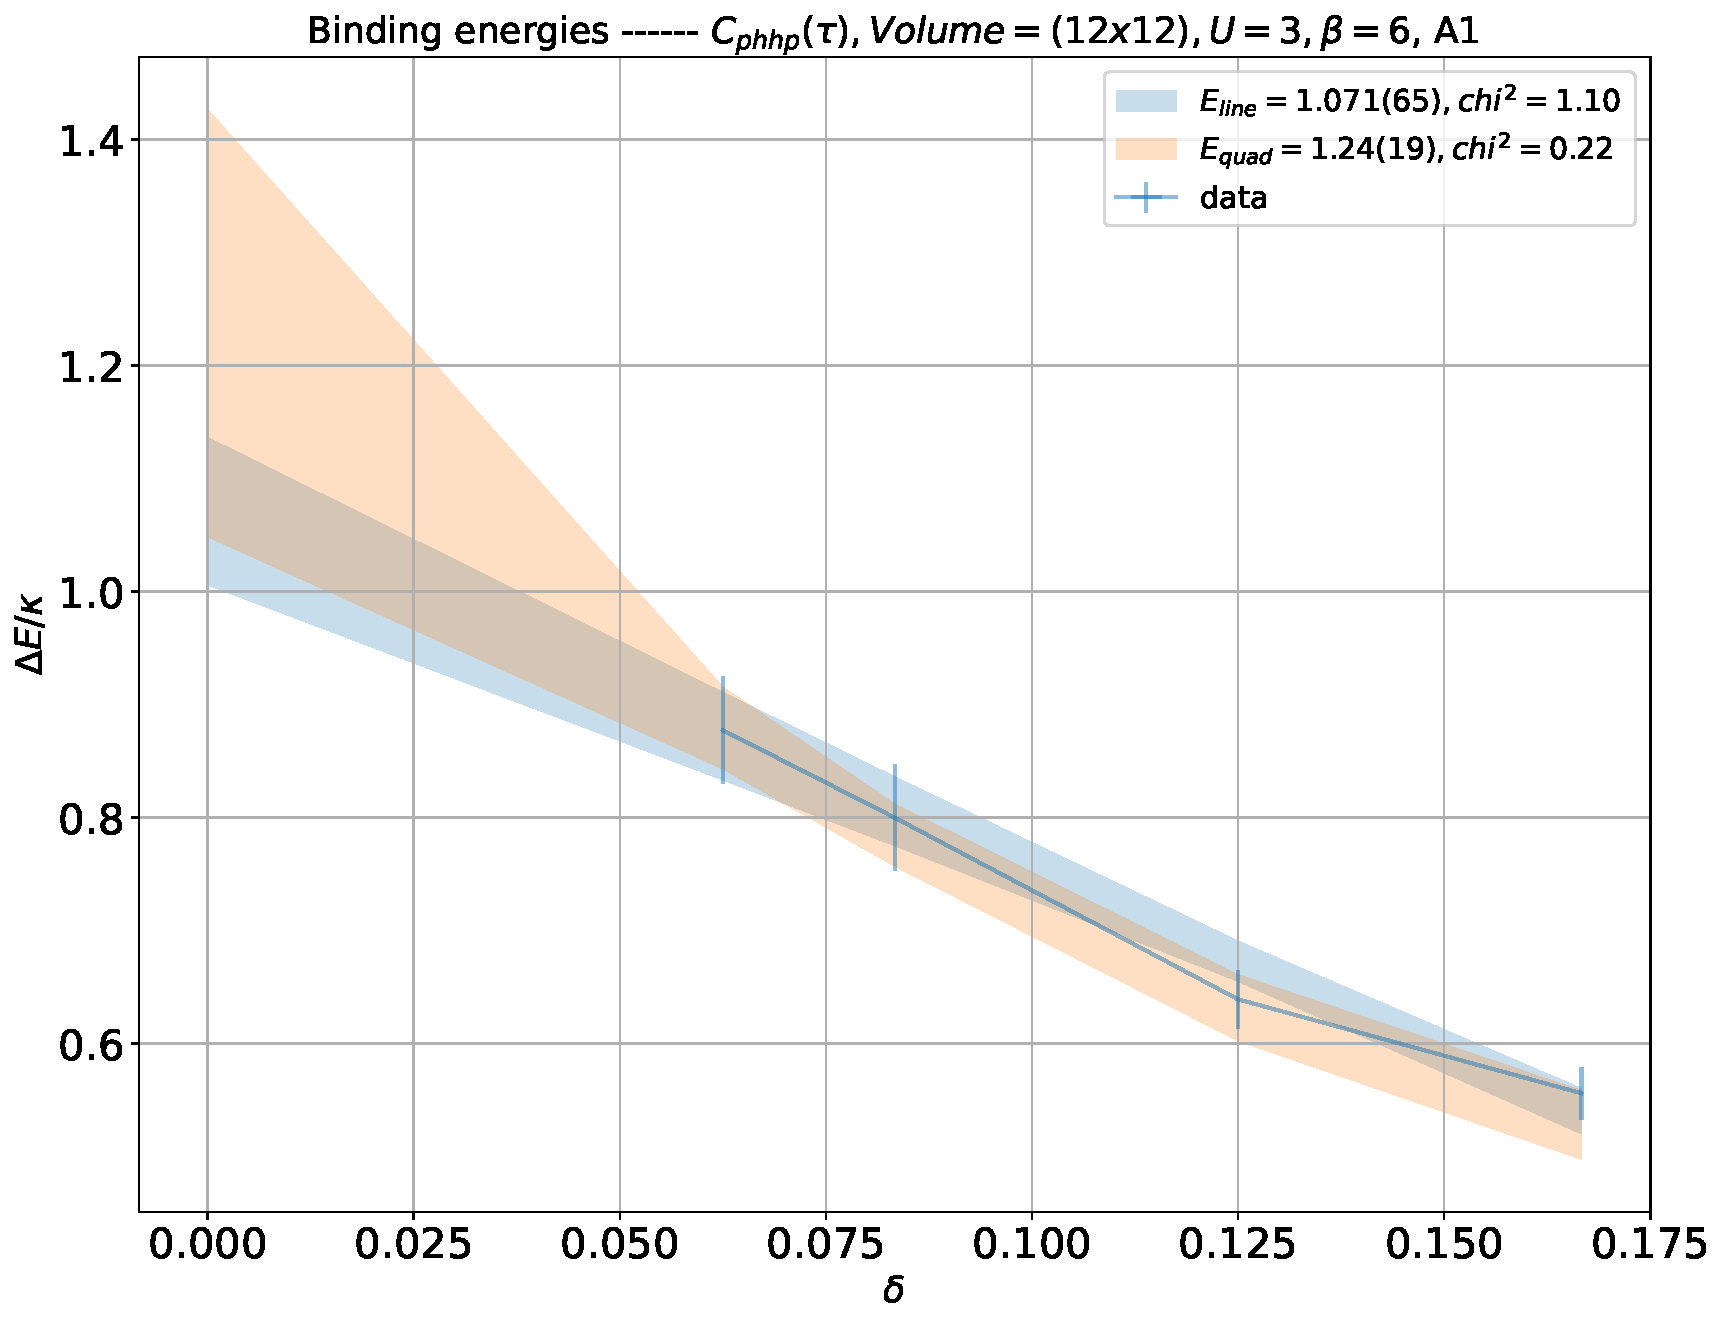
\includegraphics[width=\linewidth]{phhp-0-A1_12x12_U3_B6_cont.pdf}
  \end{subfigure}
  \begin{subfigure}{.5\textwidth}
      \centering
      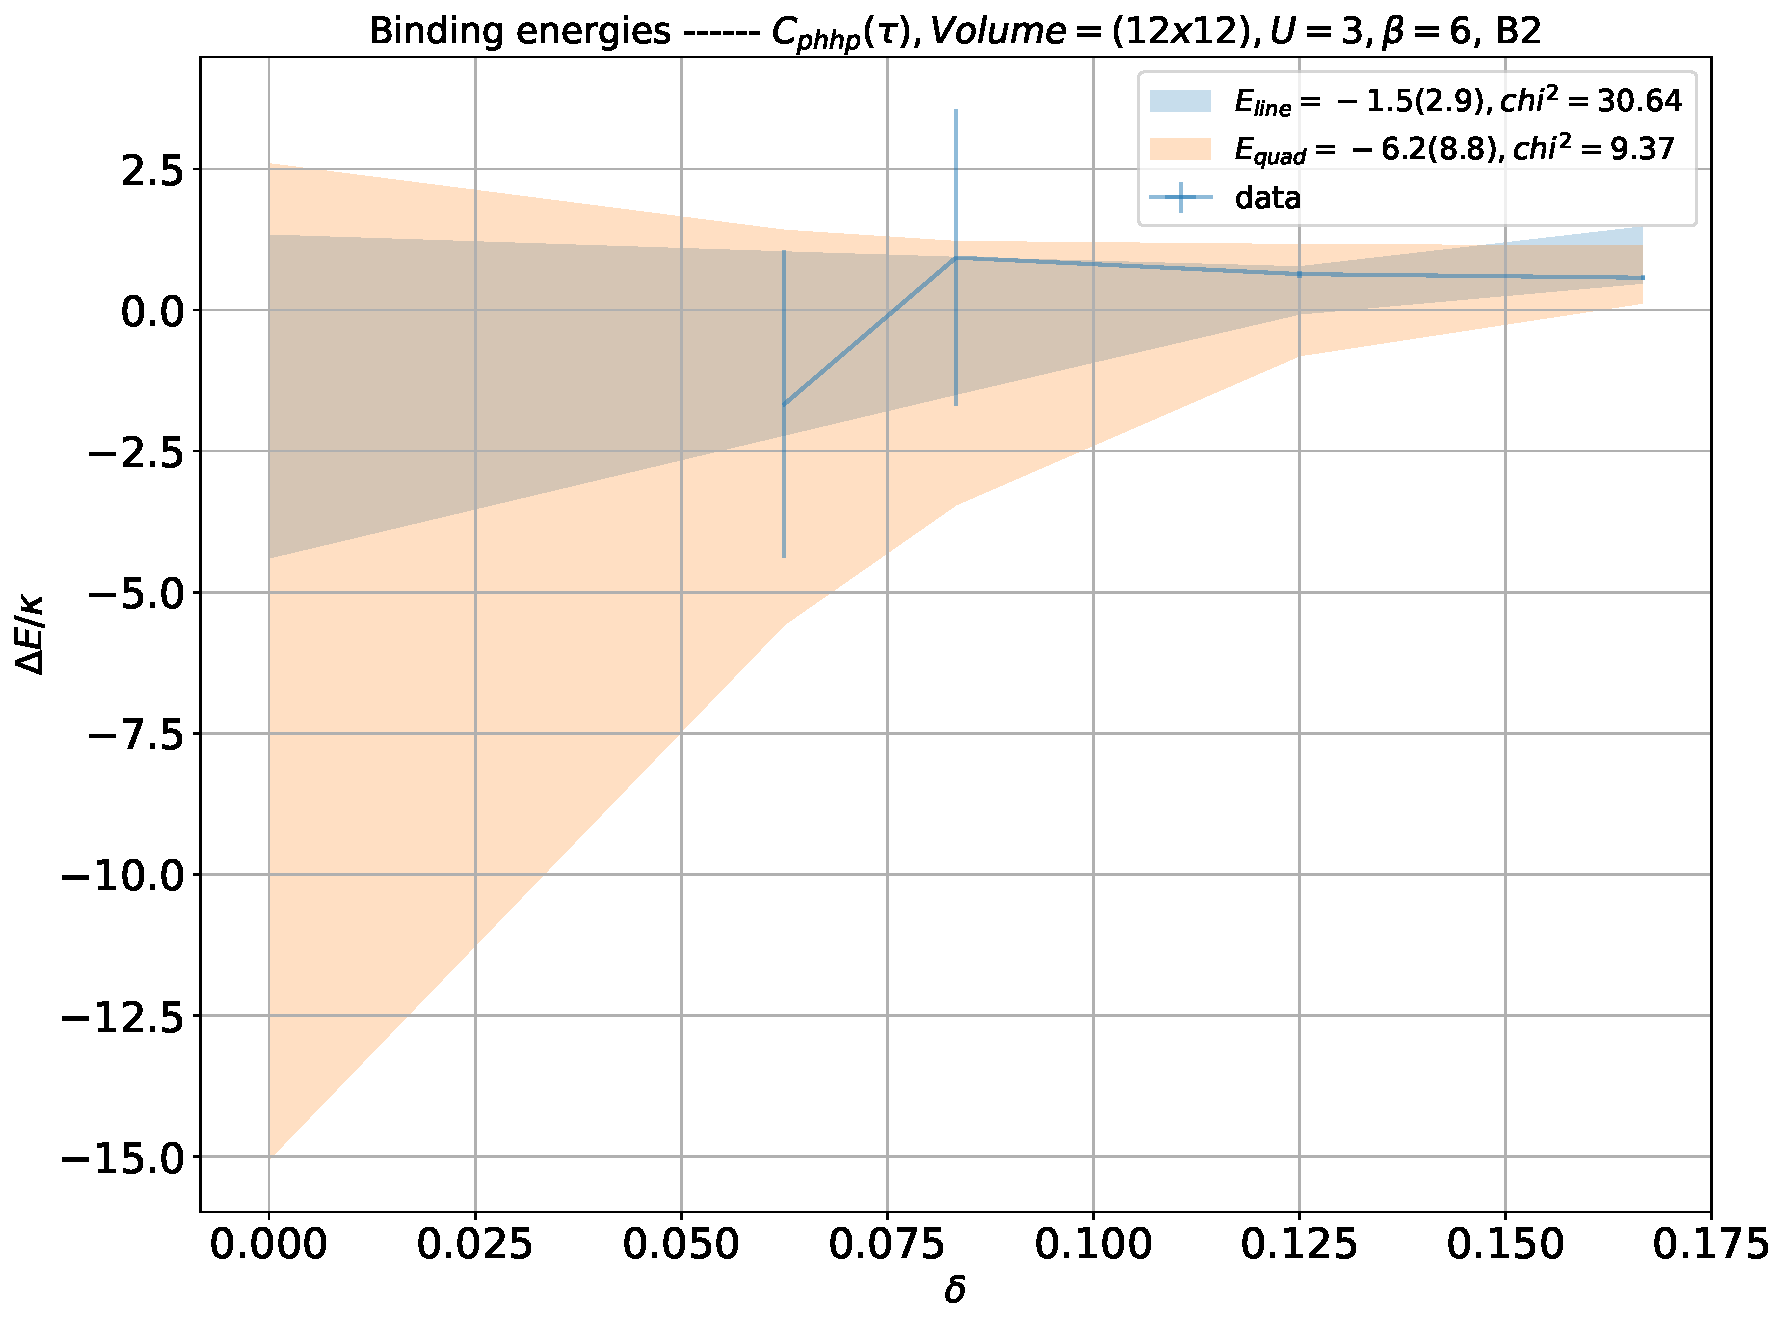
\includegraphics[width=\linewidth]{phhp-0-B2_12x12_U3_B6_cont.pdf}
  \end{subfigure}
  \caption{Binding energy extraction of the particle-hole pair at both irreducible representations, where we fit one- and two-body correlators for every $N_t$. This is followed by fitting a linear and a quadratic functions to the $\Delta E_{N_t}$ in order to extrapolate to the continuum limit ($N_t\to\infty$).}
  \label{fig:fig3}
\end{figure}

\begin{figure}
  \begin{subfigure}{.5\textwidth}
    \centering
    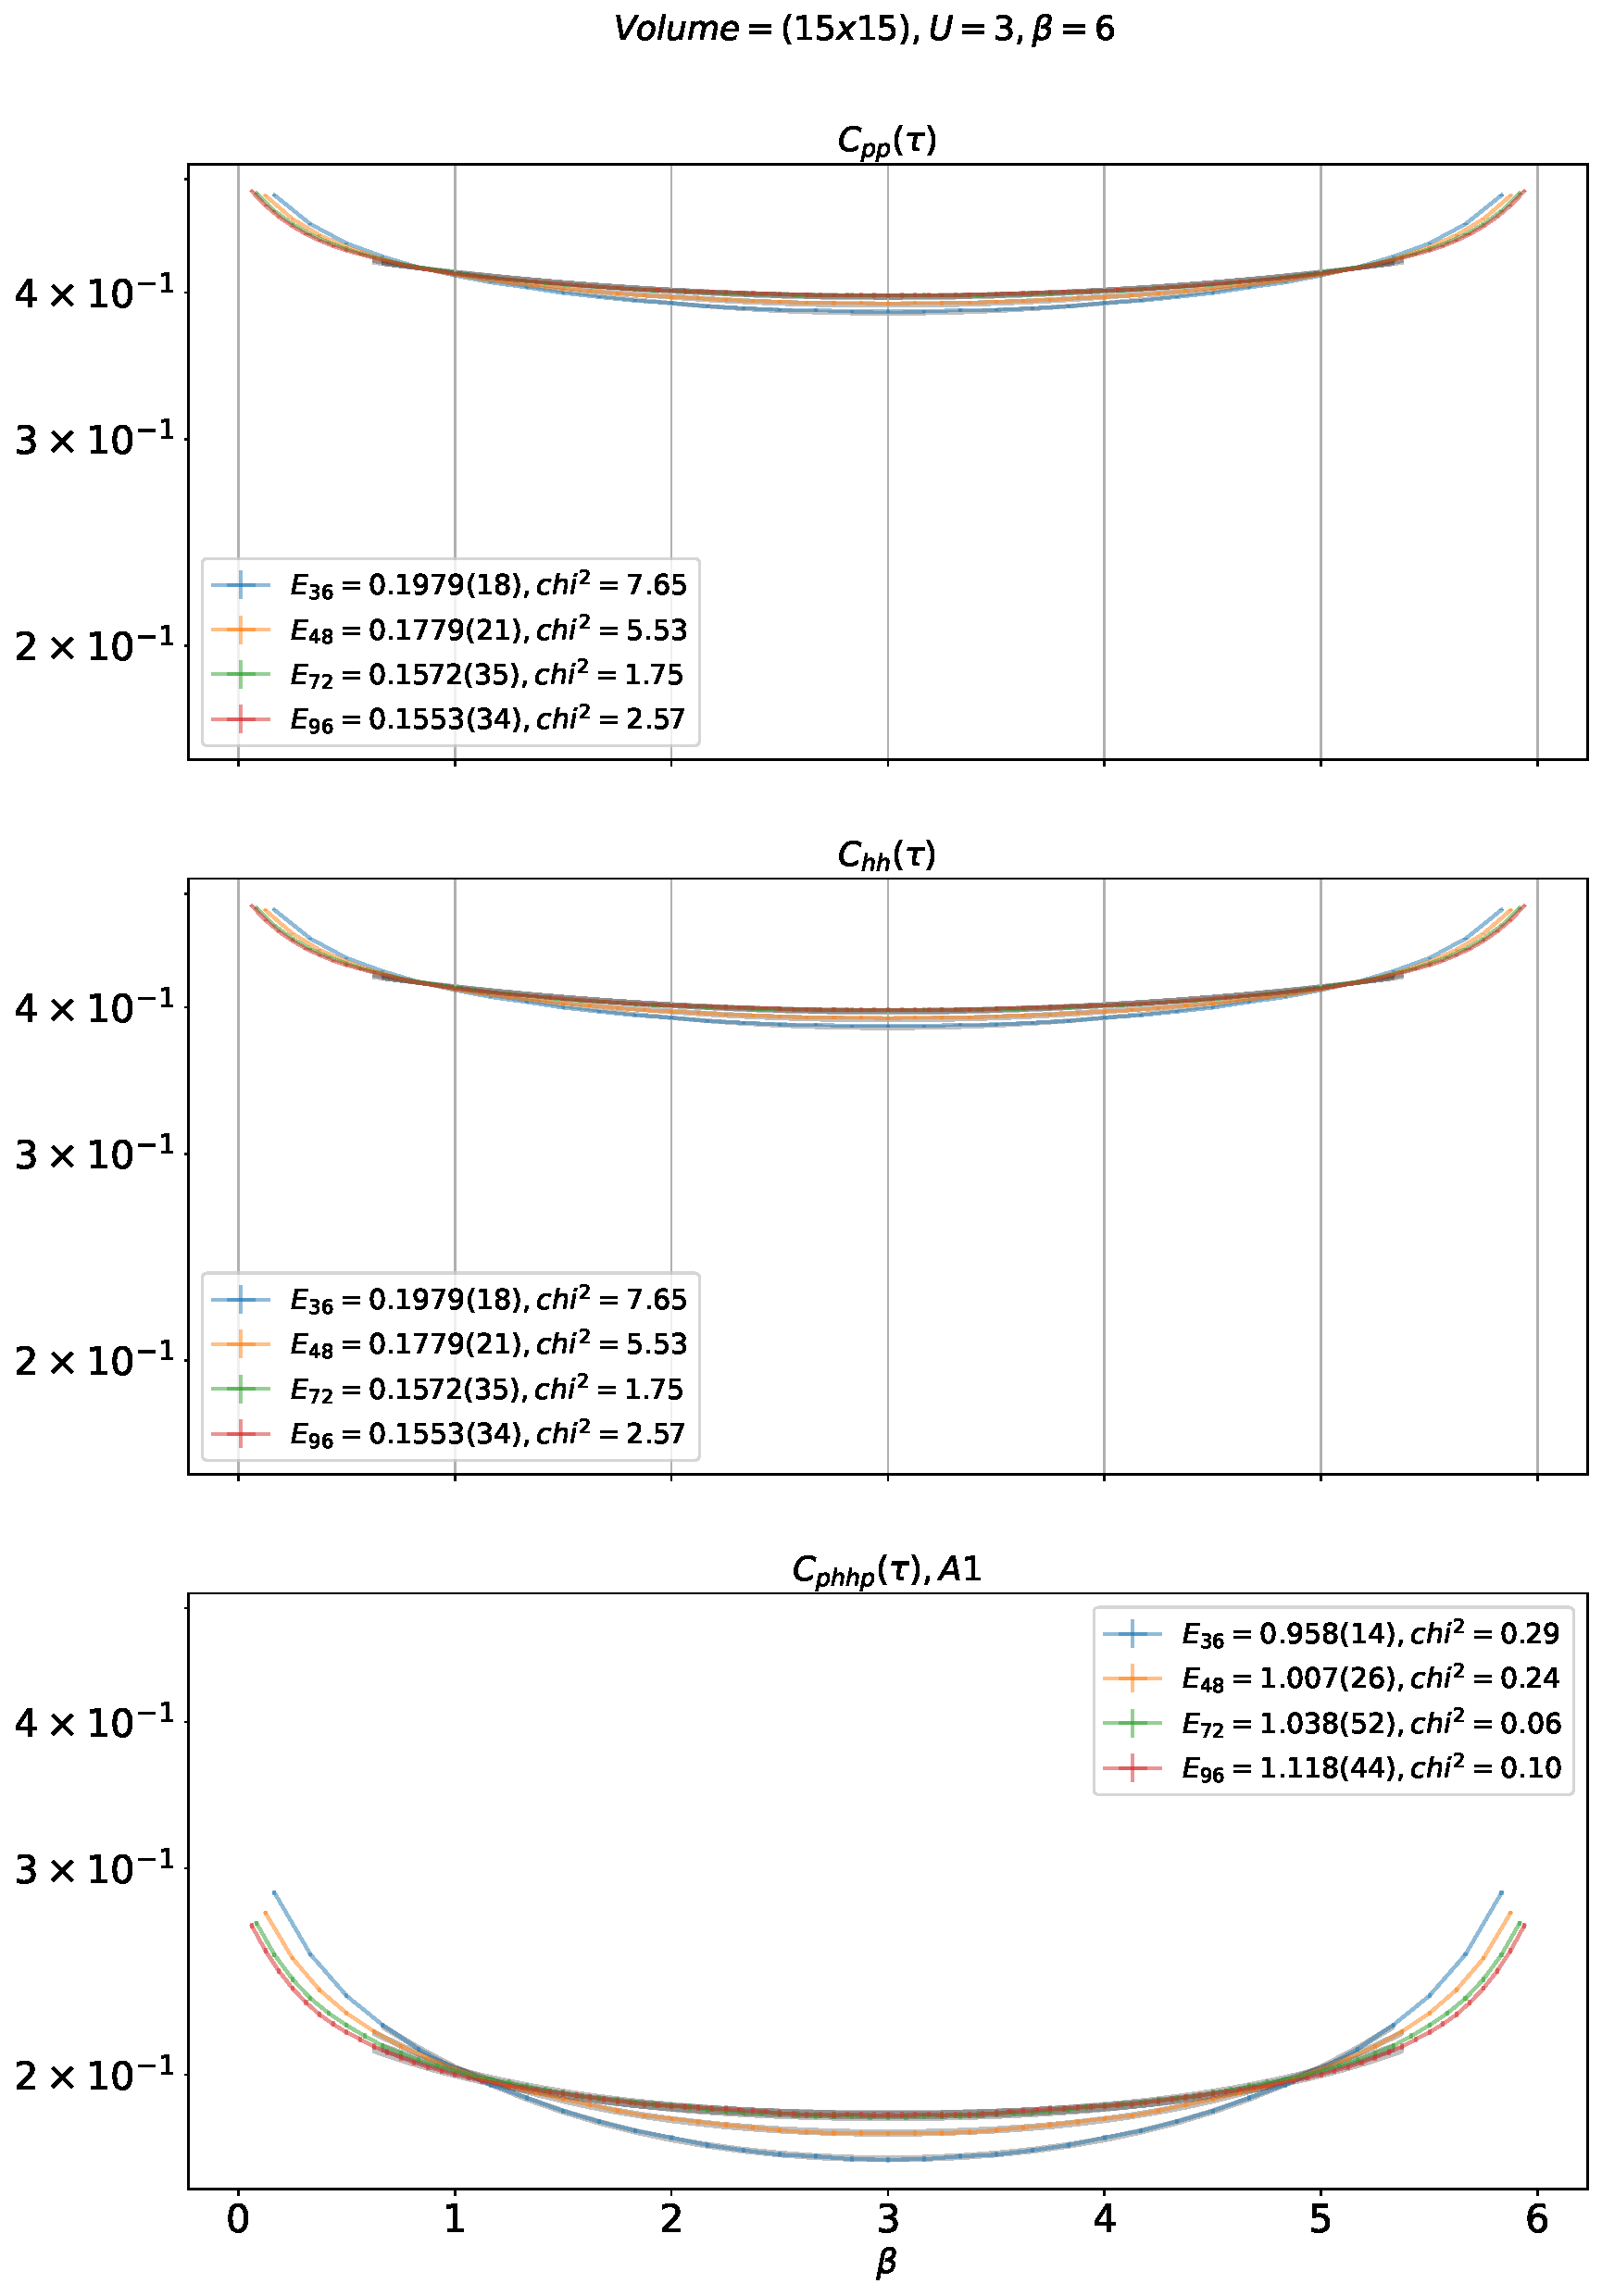
\includegraphics[width=\linewidth]{phhp-0-A1_15x15_U3_B6.pdf}
  \end{subfigure}%
  \begin{subfigure}{.5\textwidth}
    \centering
    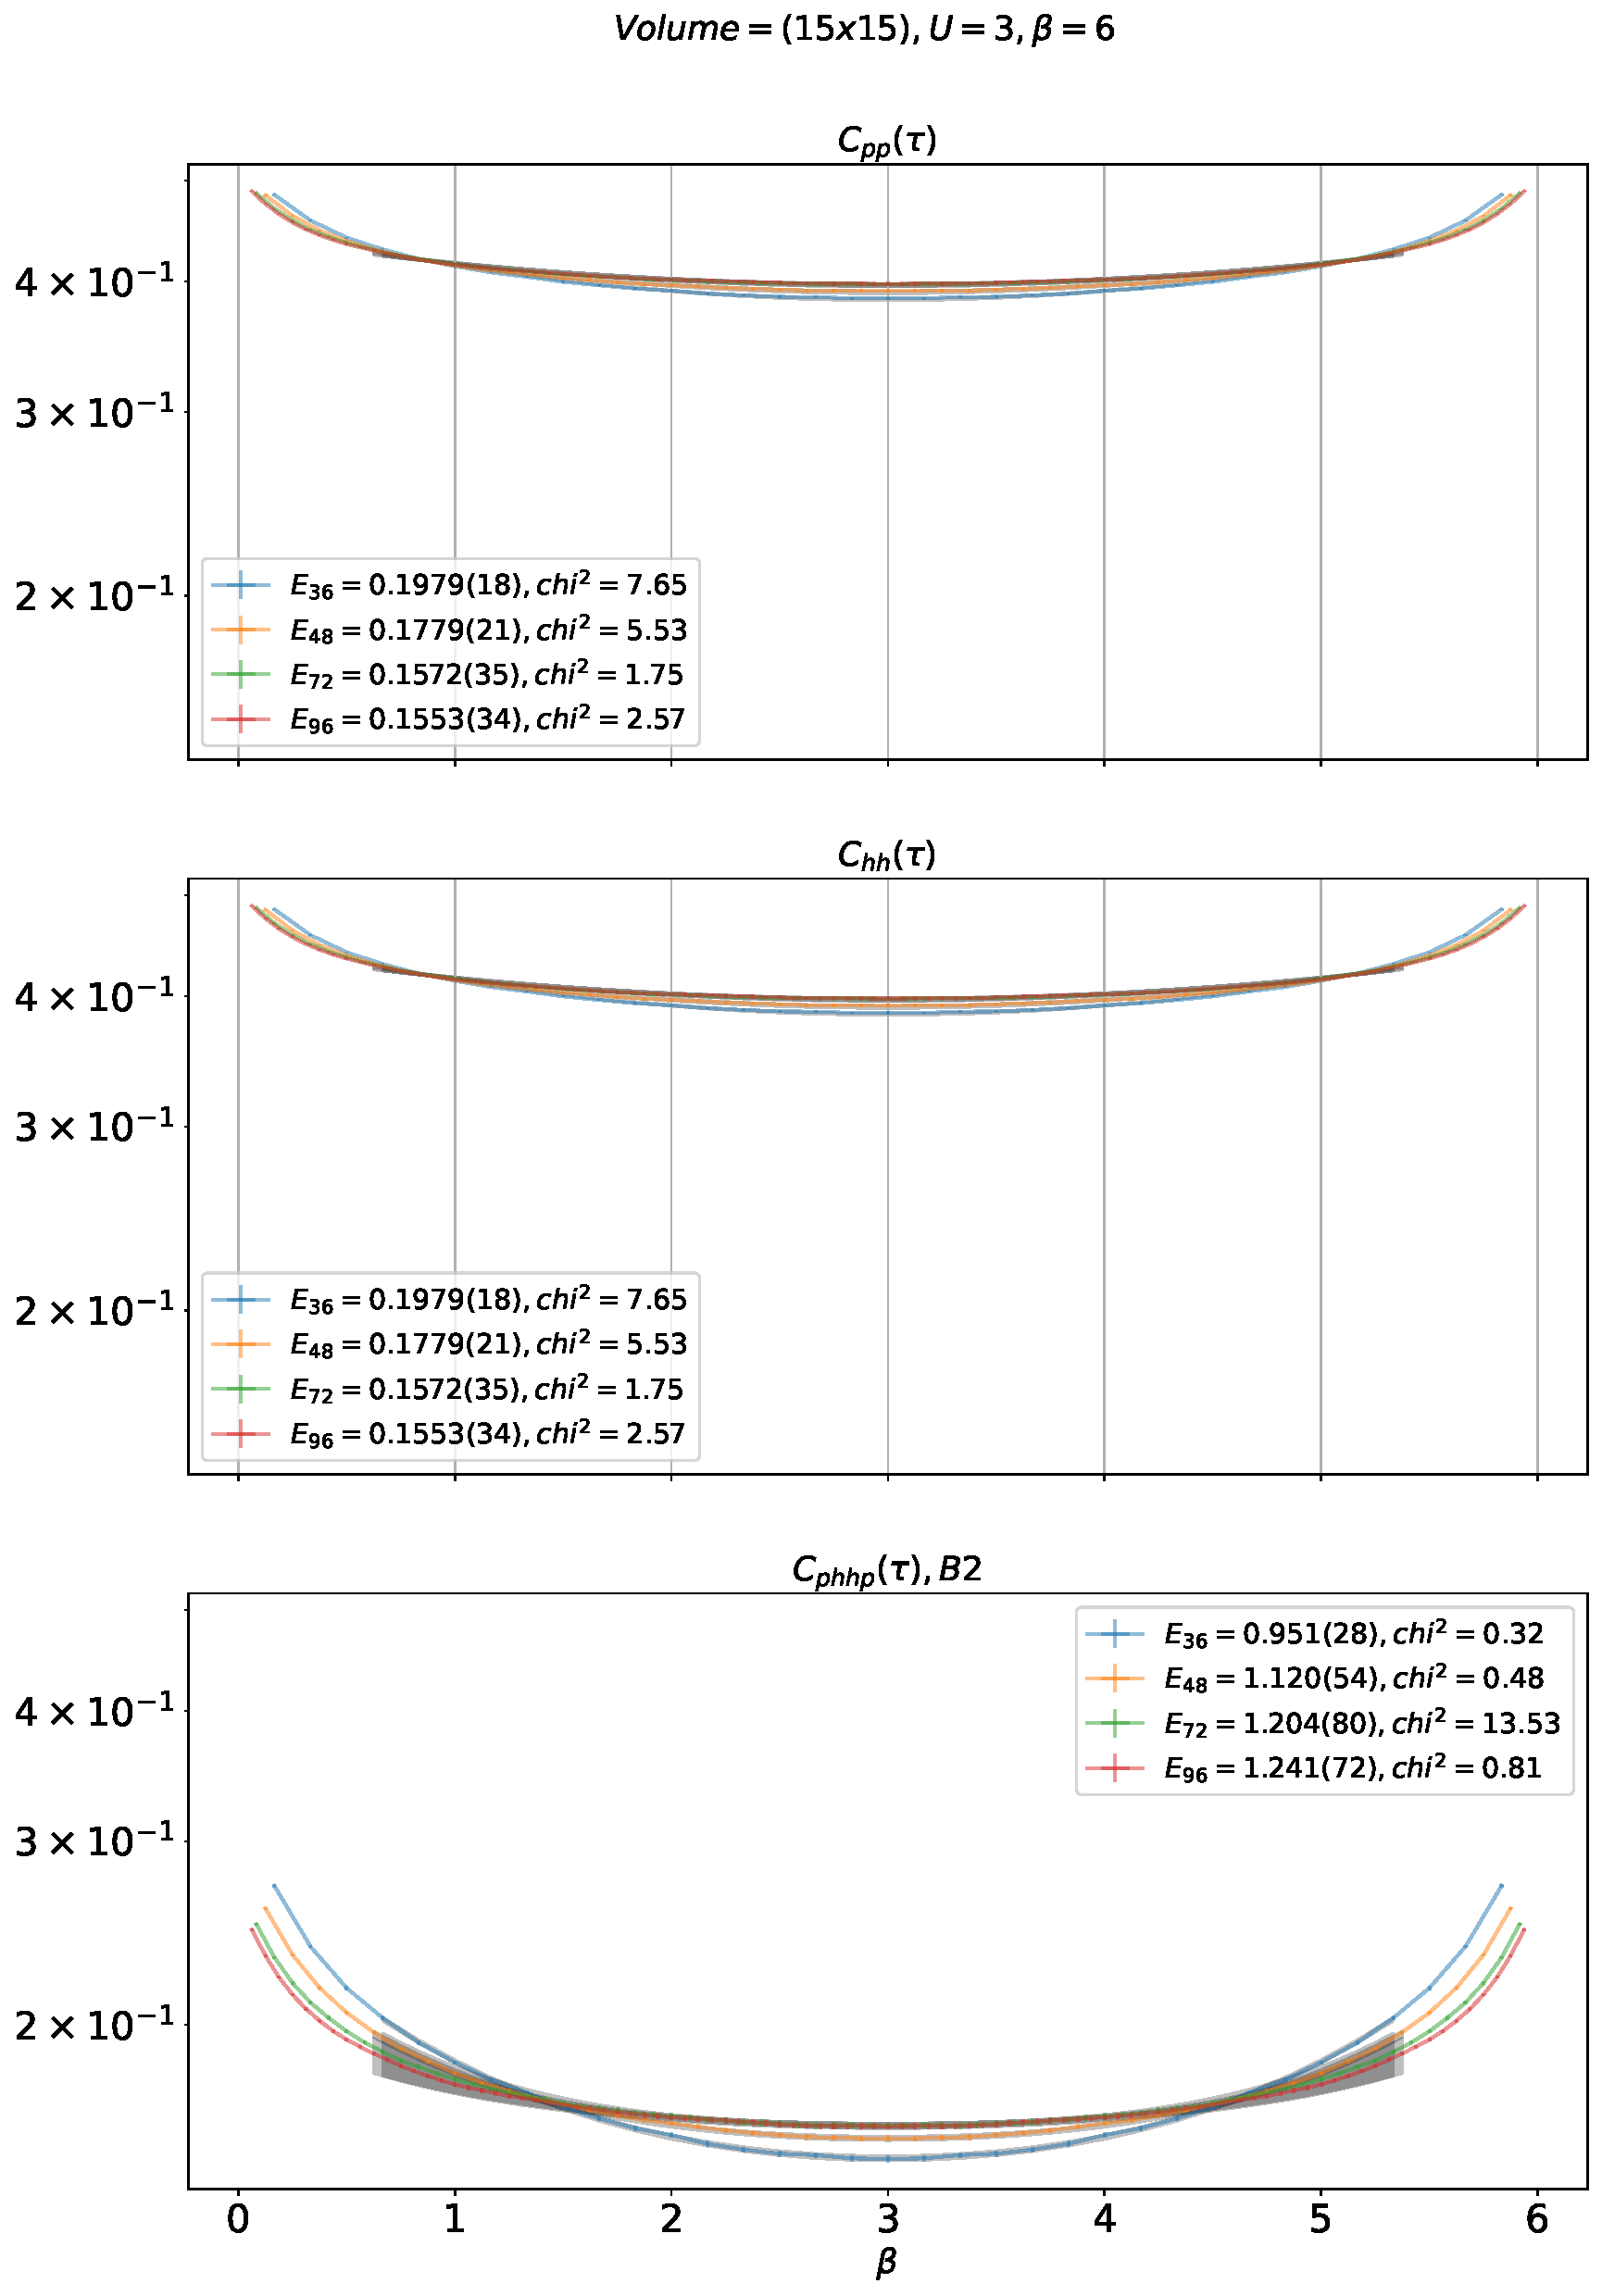
\includegraphics[width=\linewidth]{phhp-0-B2_15x15_U3_B6.pdf}
  \end{subfigure}
  \begin{subfigure}{.5\textwidth}
      \centering
      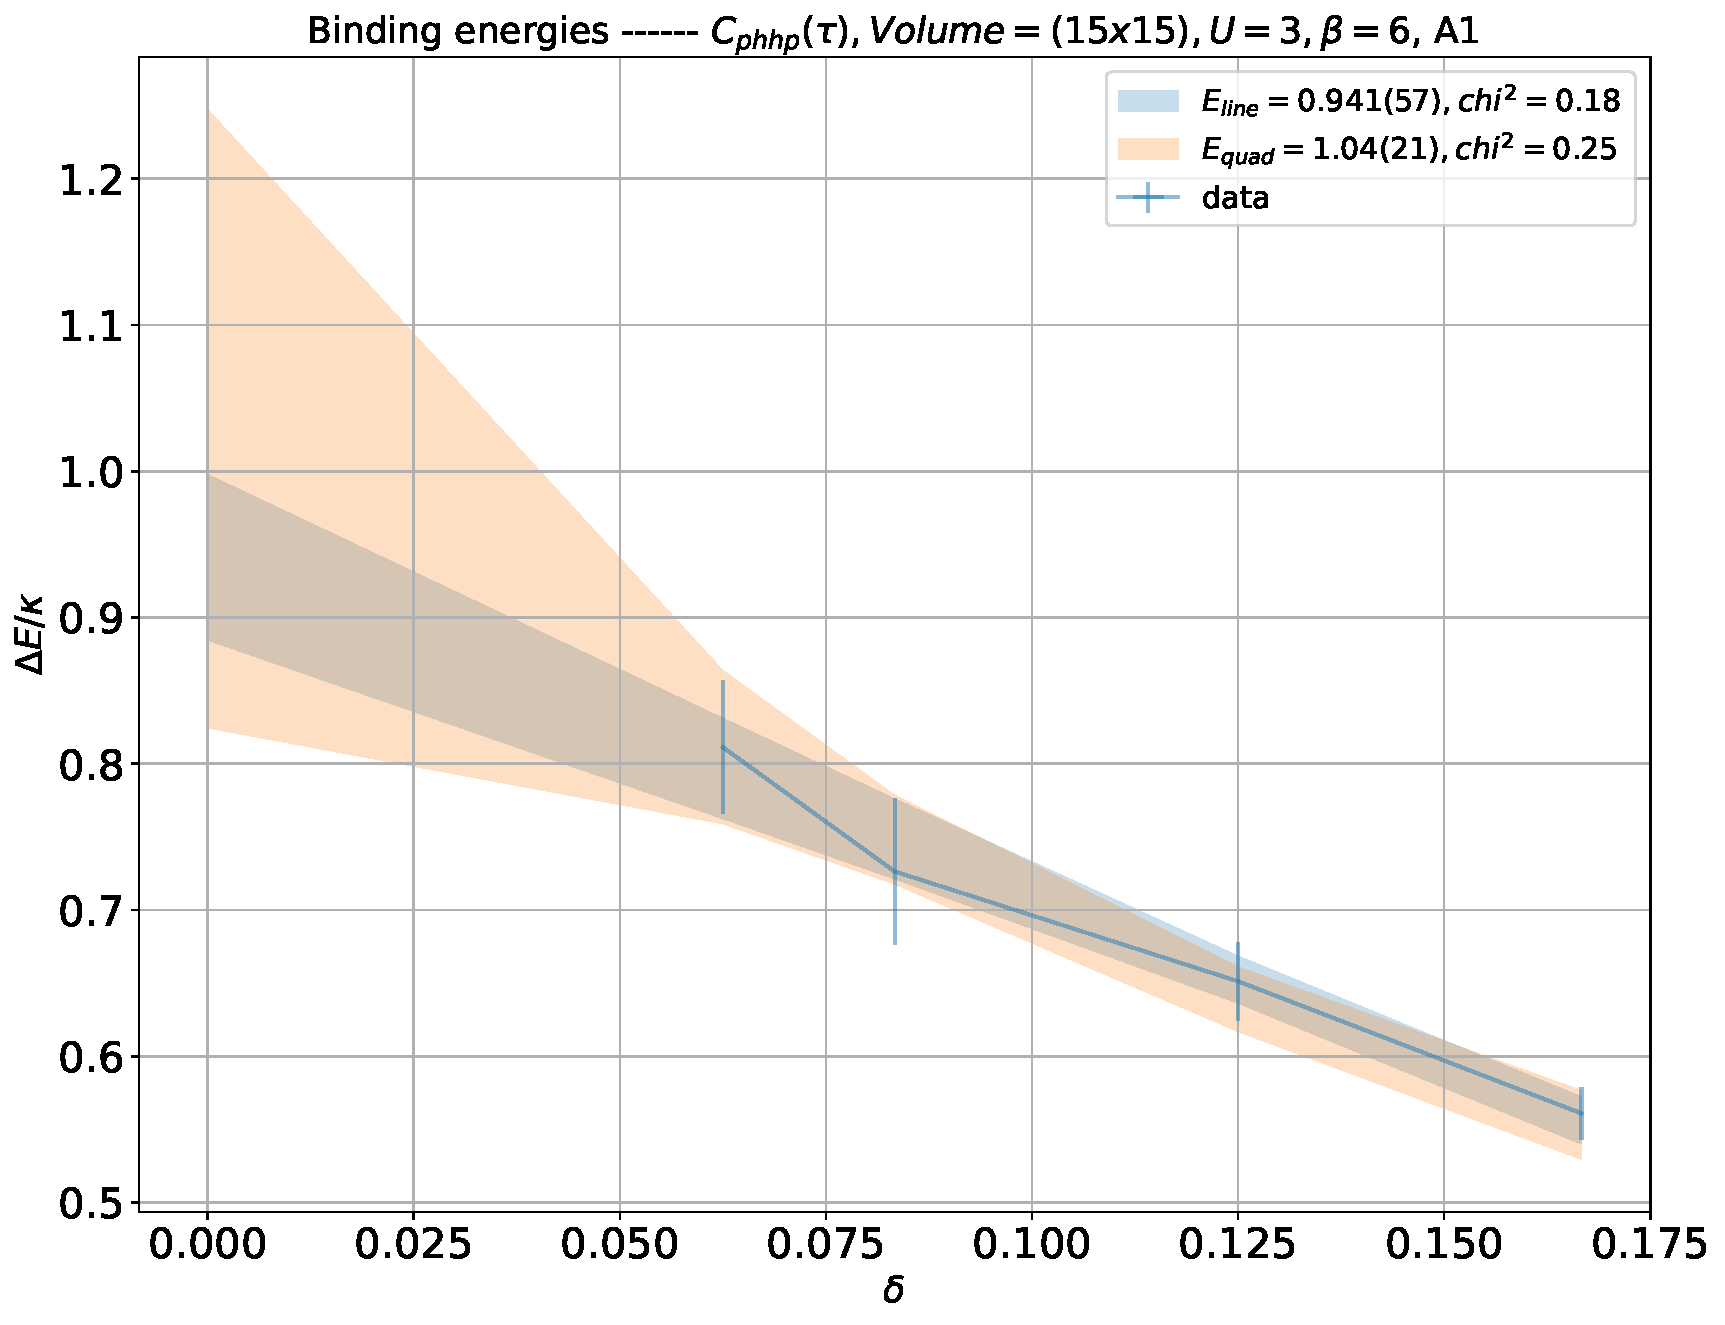
\includegraphics[width=\linewidth]{phhp-0-A1_15x15_U3_B6_cont.pdf}
  \end{subfigure}
  \begin{subfigure}{.5\textwidth}
      \centering
      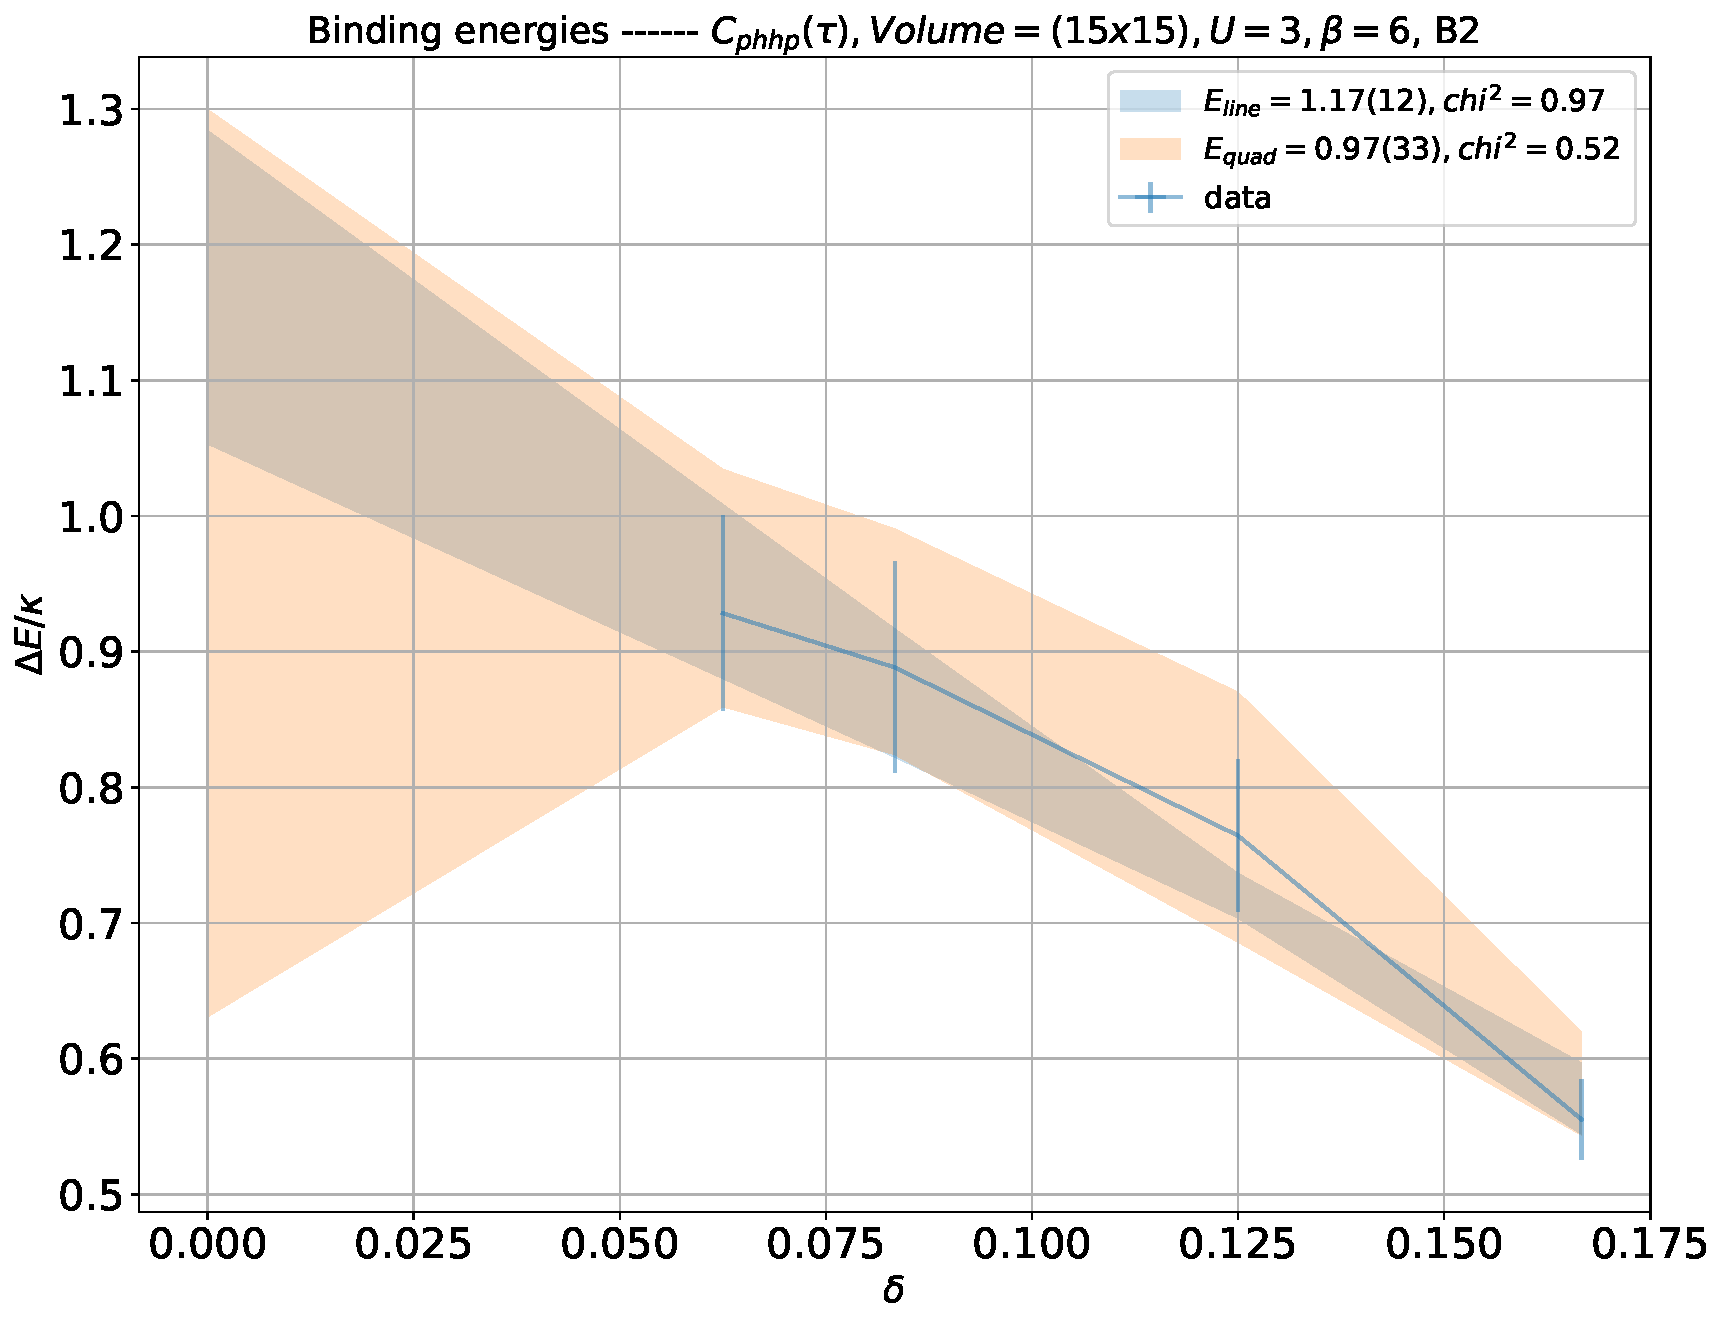
\includegraphics[width=\linewidth]{phhp-0-B2_15x15_U3_B6_cont.pdf}
  \end{subfigure}
  \caption{Binding energy extraction of the particle-hole pair at both irreducible representations, where we fit one- and two-body correlators for every $N_t$. This is followed by fitting a linear and a quadratic functions to the $\Delta E_{N_t}$ in order to extrapolate to the continuum limit ($N_t\to\infty$).}
  \label{fig:fig4}
\end{figure}

\begin{figure}
  \begin{subfigure}{.5\textwidth}
    \centering
    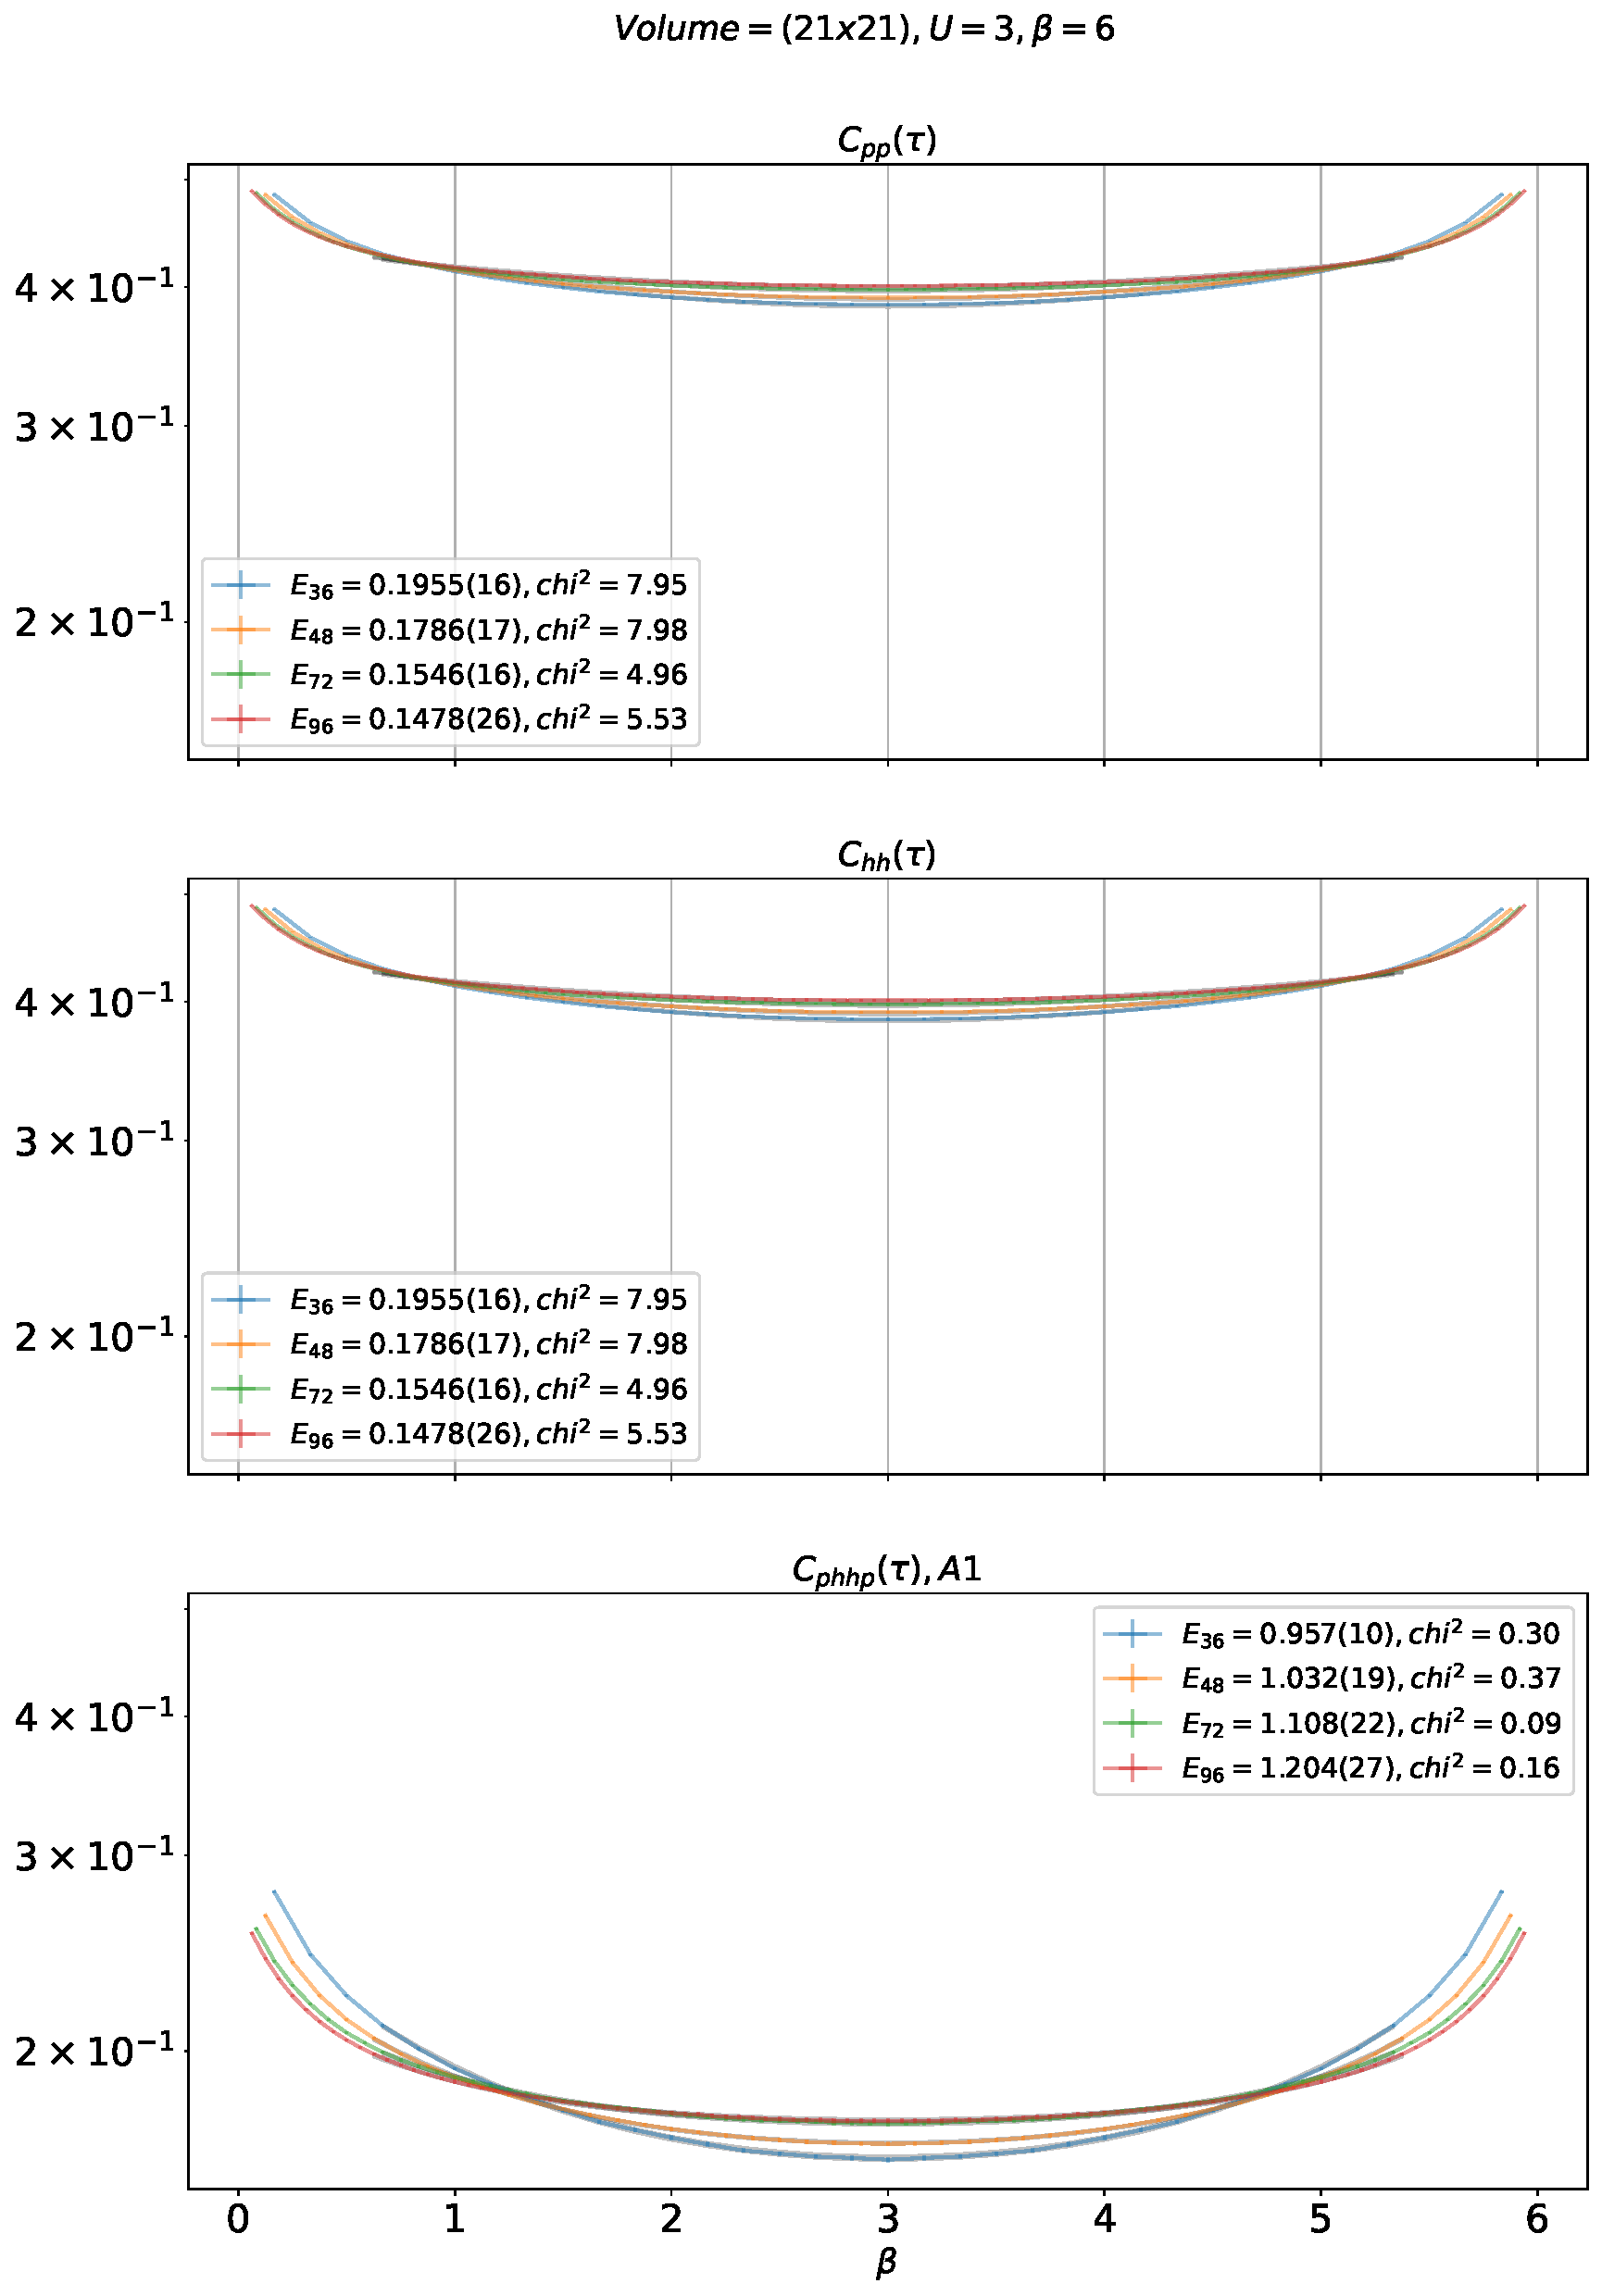
\includegraphics[width=\linewidth]{phhp-0-A1_21x21_U3_B6.pdf}
  \end{subfigure}%
  \begin{subfigure}{.5\textwidth}
    \centering
    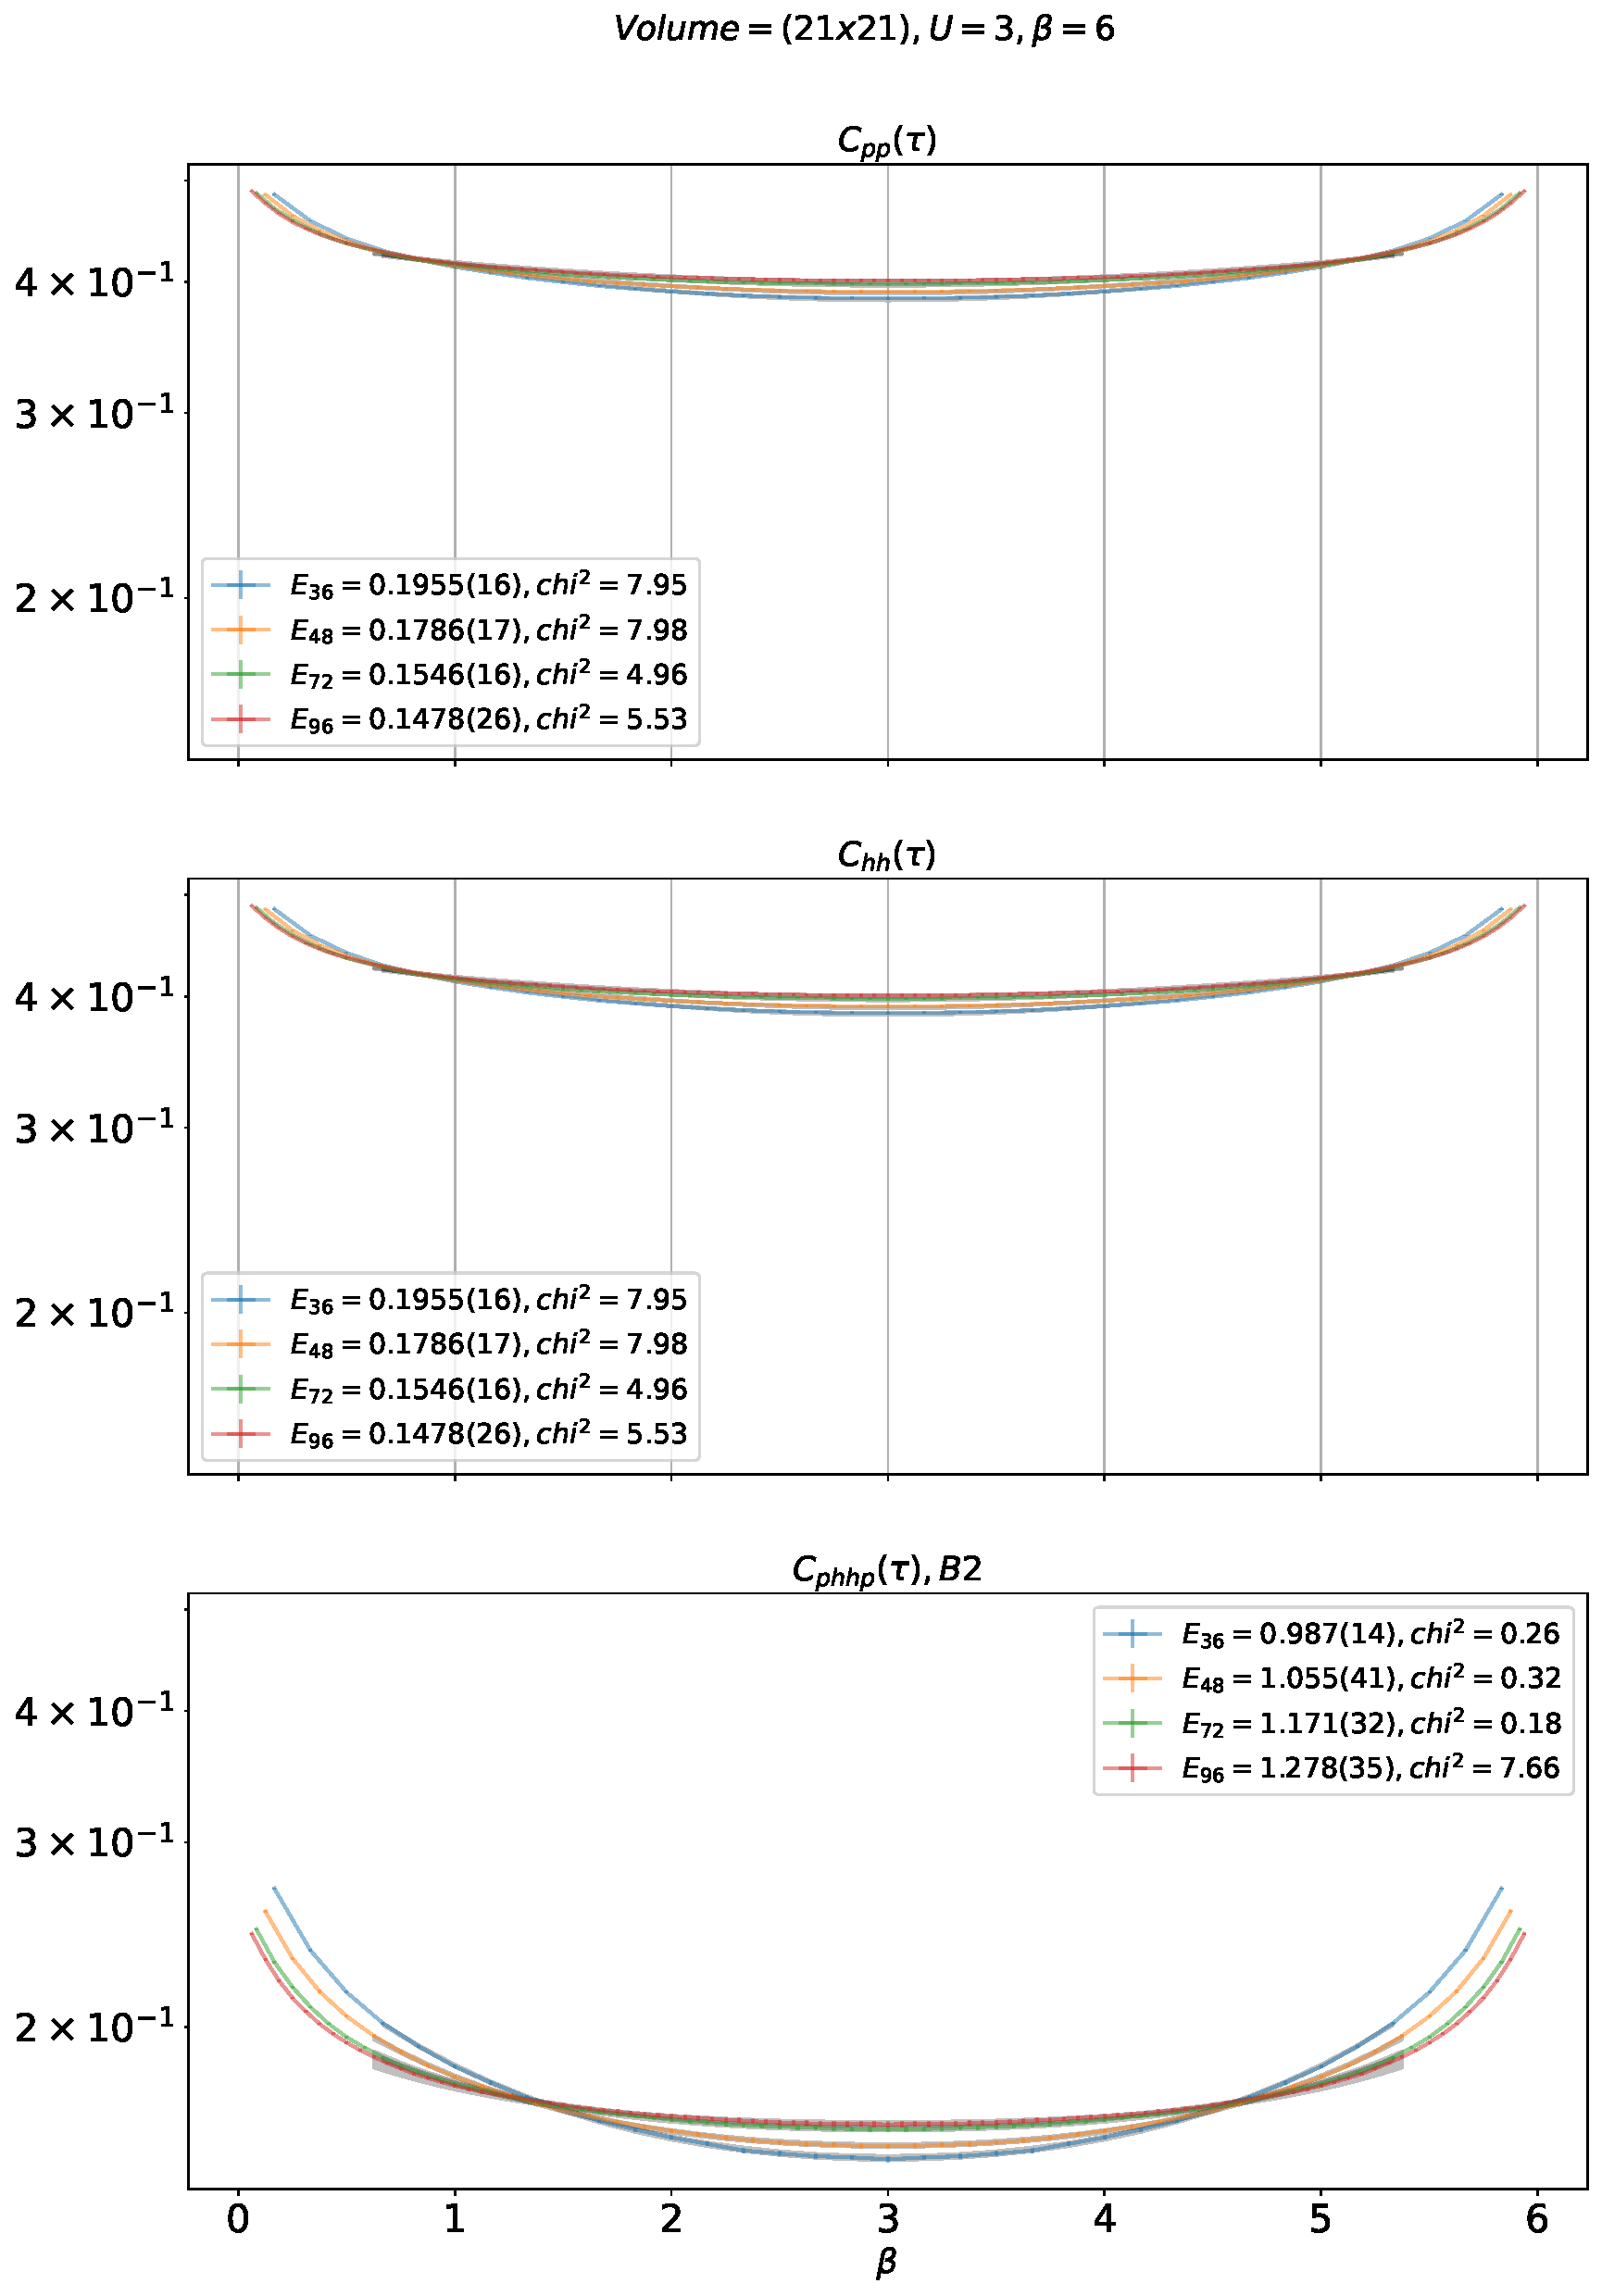
\includegraphics[width=\linewidth]{phhp-0-B2_21x21_U3_B6.pdf}
  \end{subfigure}
  \begin{subfigure}{.5\textwidth}
      \centering
      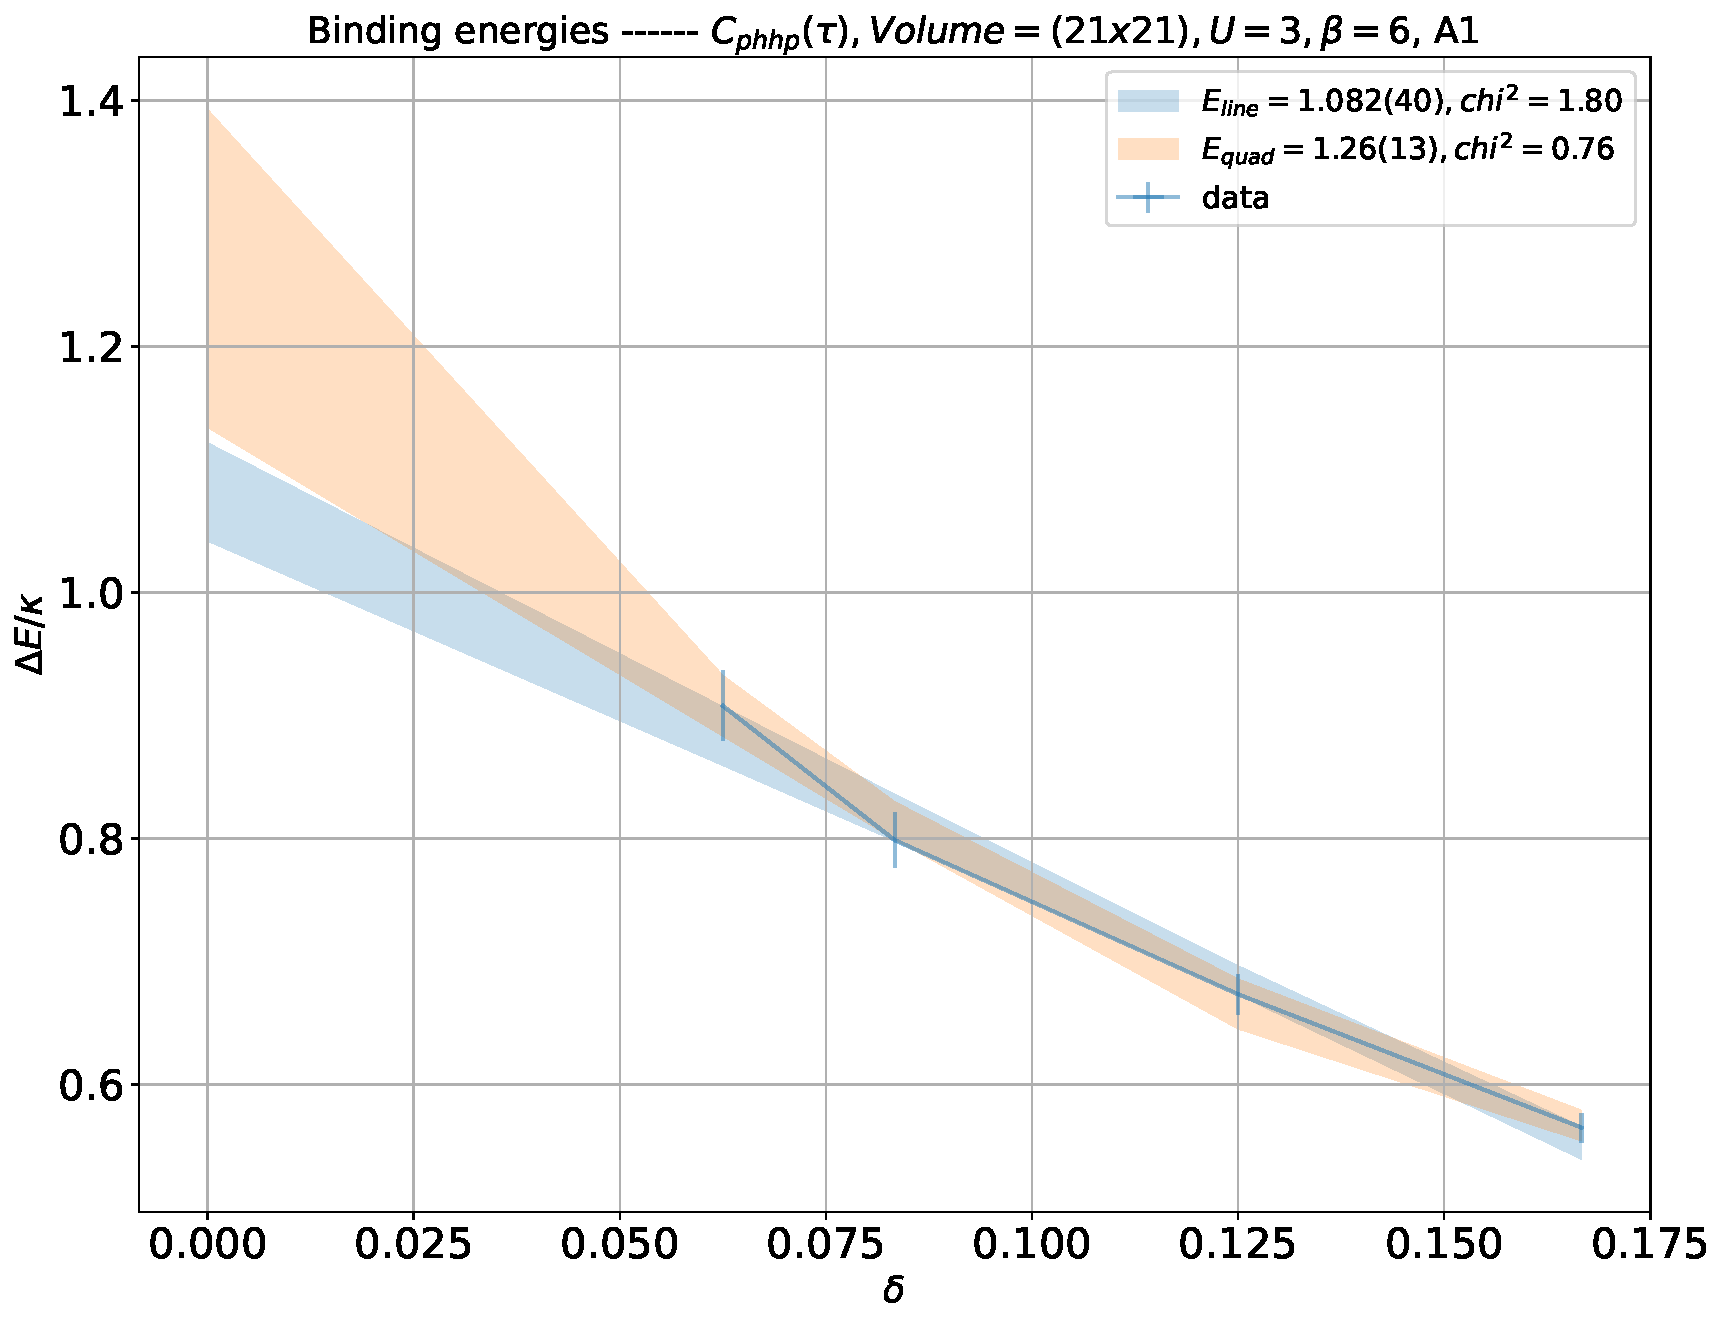
\includegraphics[width=\linewidth]{phhp-0-A1_21x21_U3_B6_cont.pdf}
  \end{subfigure}
  \begin{subfigure}{.5\textwidth}
      \centering
      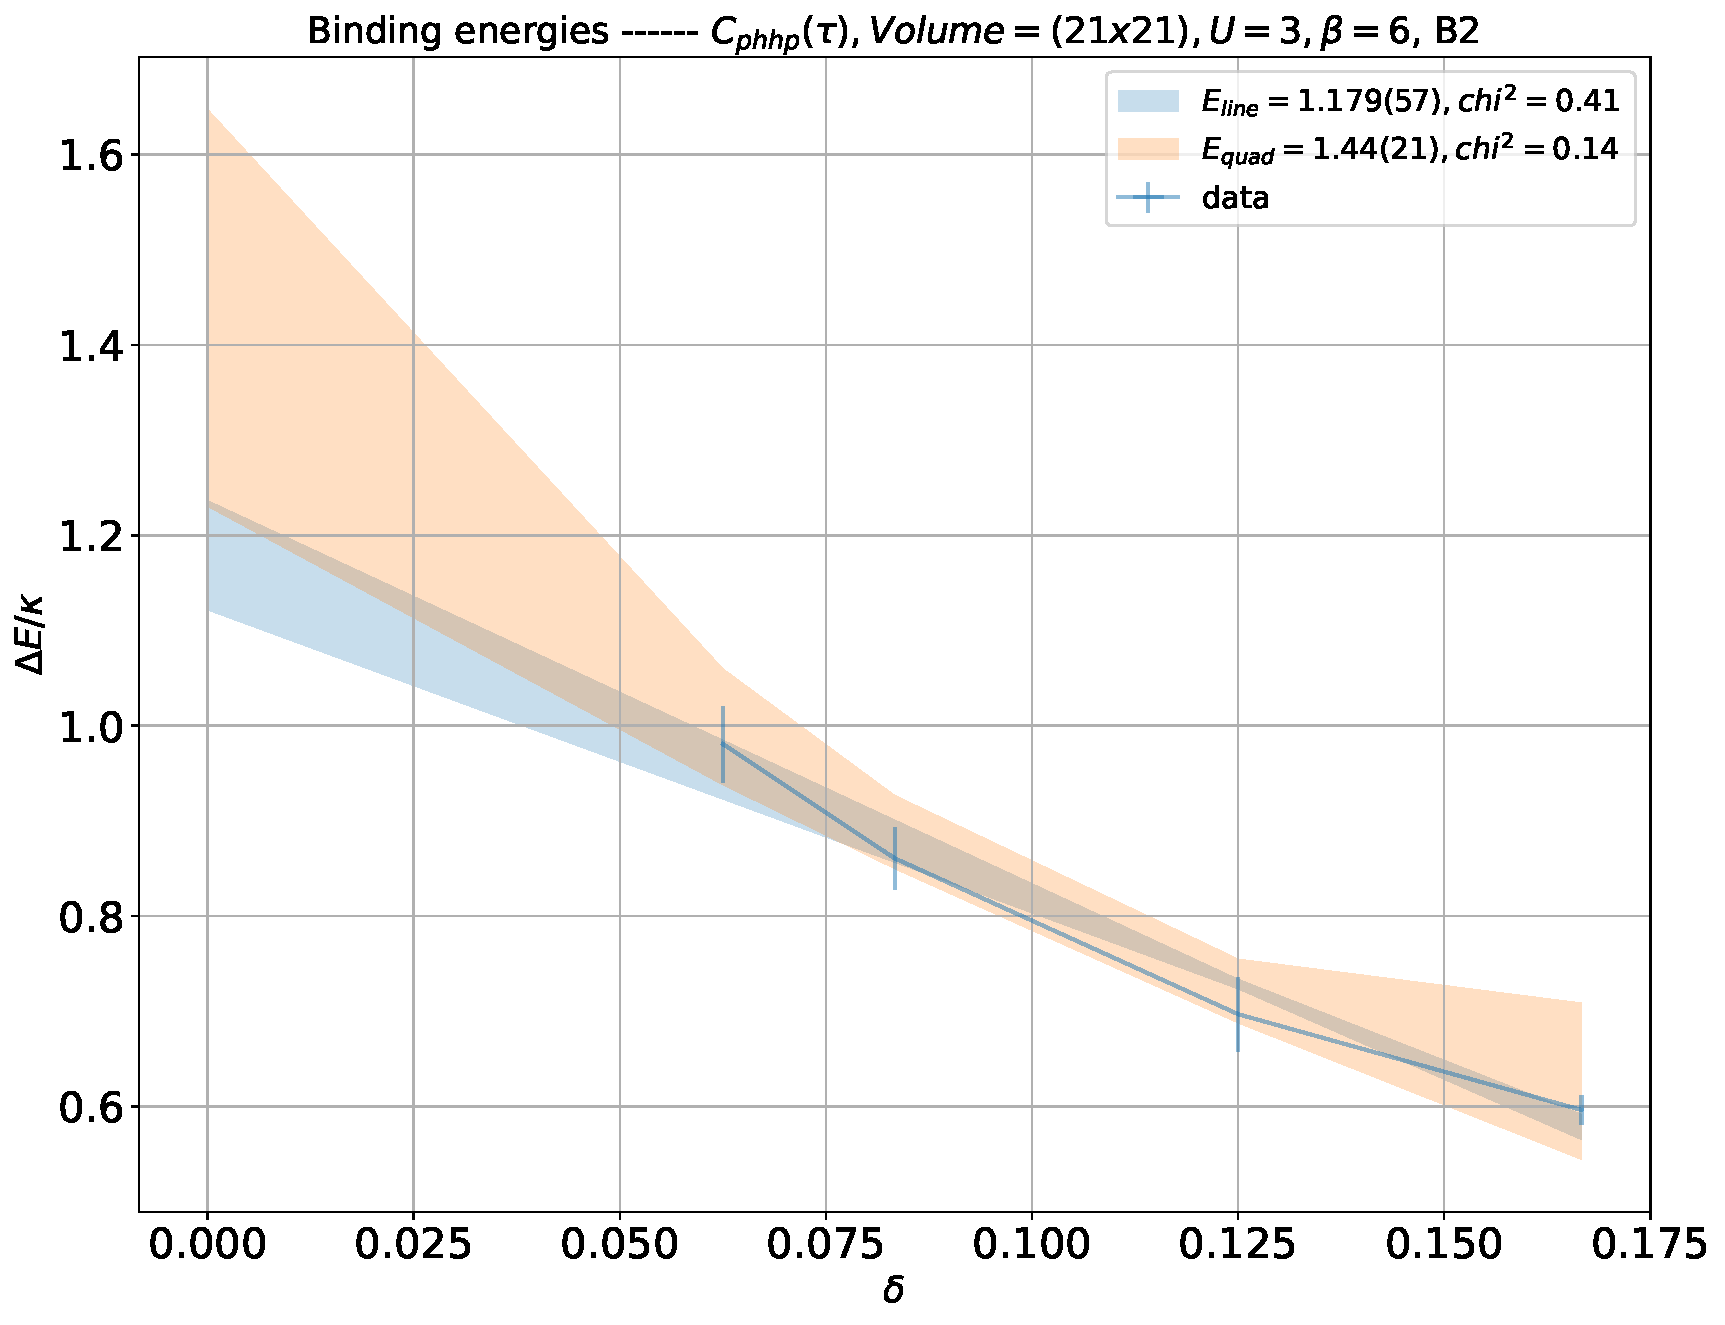
\includegraphics[width=\linewidth]{phhp-0-B2_21x21_U3_B6_cont.pdf}
  \end{subfigure}
  \caption{Binding energy extraction of the particle-hole pair at both irreducible representations, where we fit one- and two-body correlators for every $N_t$. This is followed by fitting a linear and a quadratic functions to the $\Delta E_{N_t}$ in order to extrapolate to the continuum limit ($N_t\to\infty$).}
  \label{fig:fig5}
\end{figure}

\begin{figure}
  \begin{subfigure}{.5\textwidth}
    \centering
    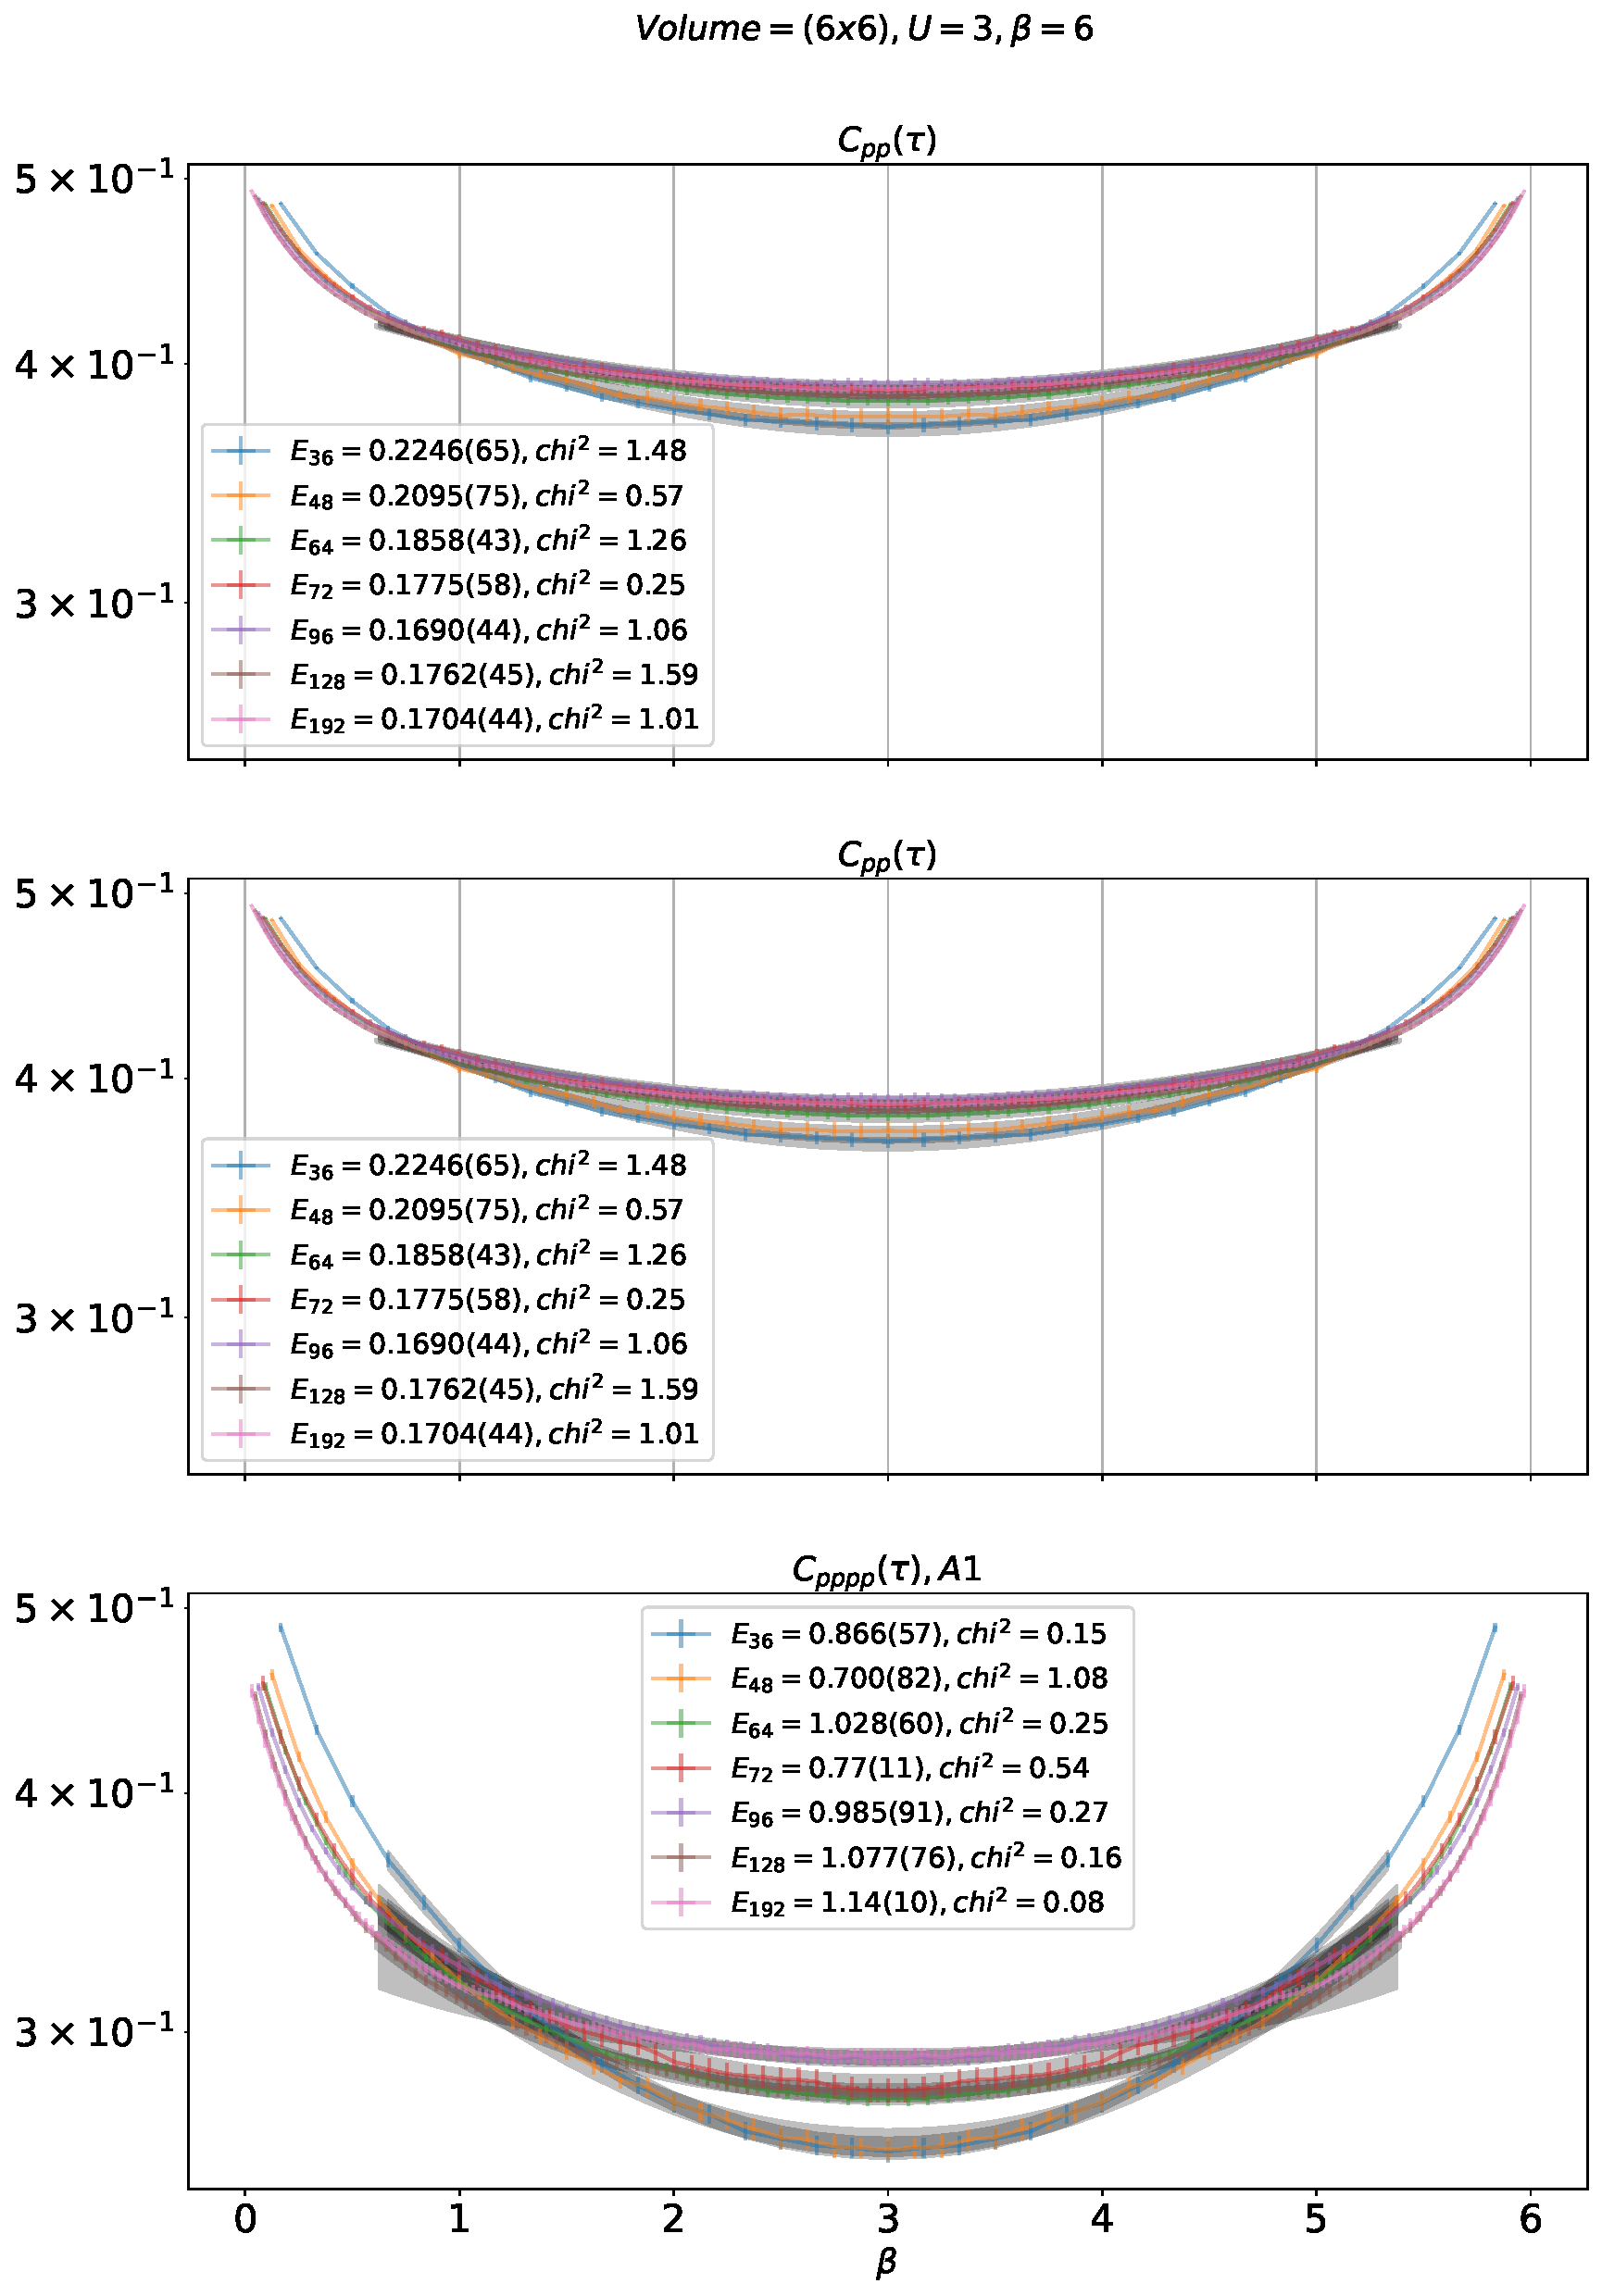
\includegraphics[width=\linewidth]{pppp-0-A1_6x6_U3.0_B6.0.pdf}
  \end{subfigure}%
  \begin{subfigure}{.5\textwidth}
    \centering
    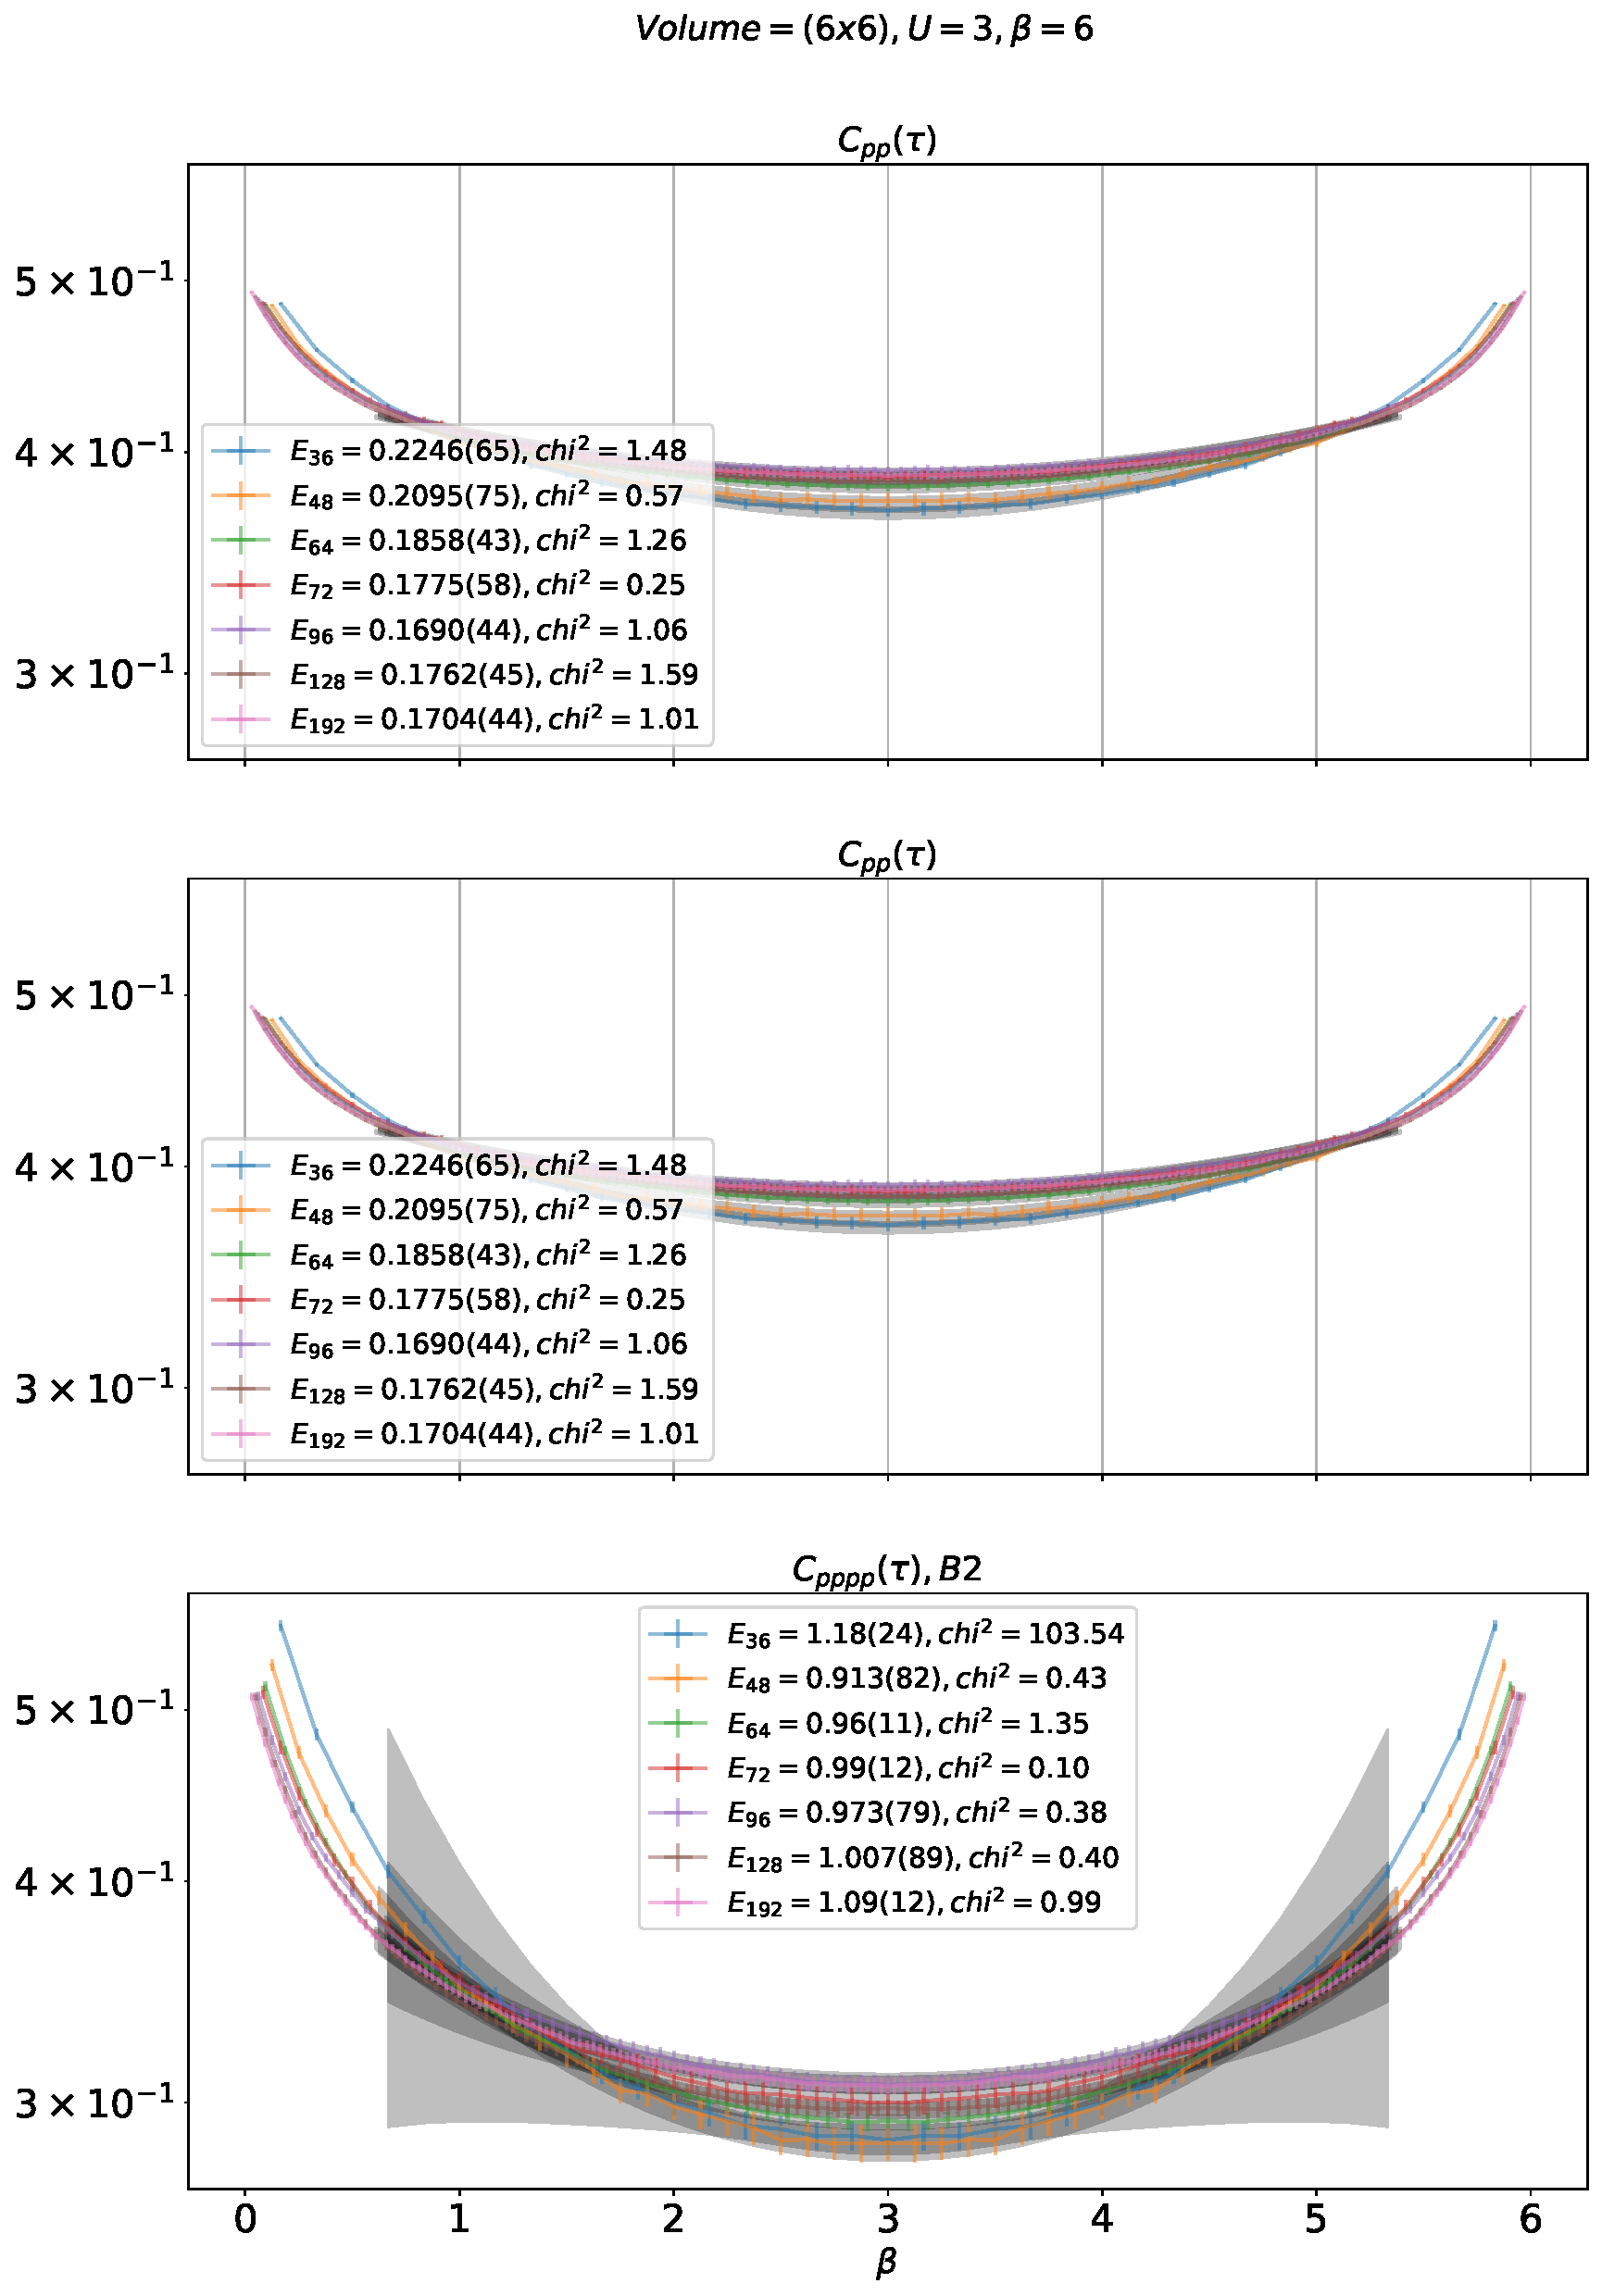
\includegraphics[width=\linewidth]{pppp-0-B2_6x6_U3.0_B6.0.pdf}
  \end{subfigure}
  \begin{subfigure}{.5\textwidth}
      \centering
      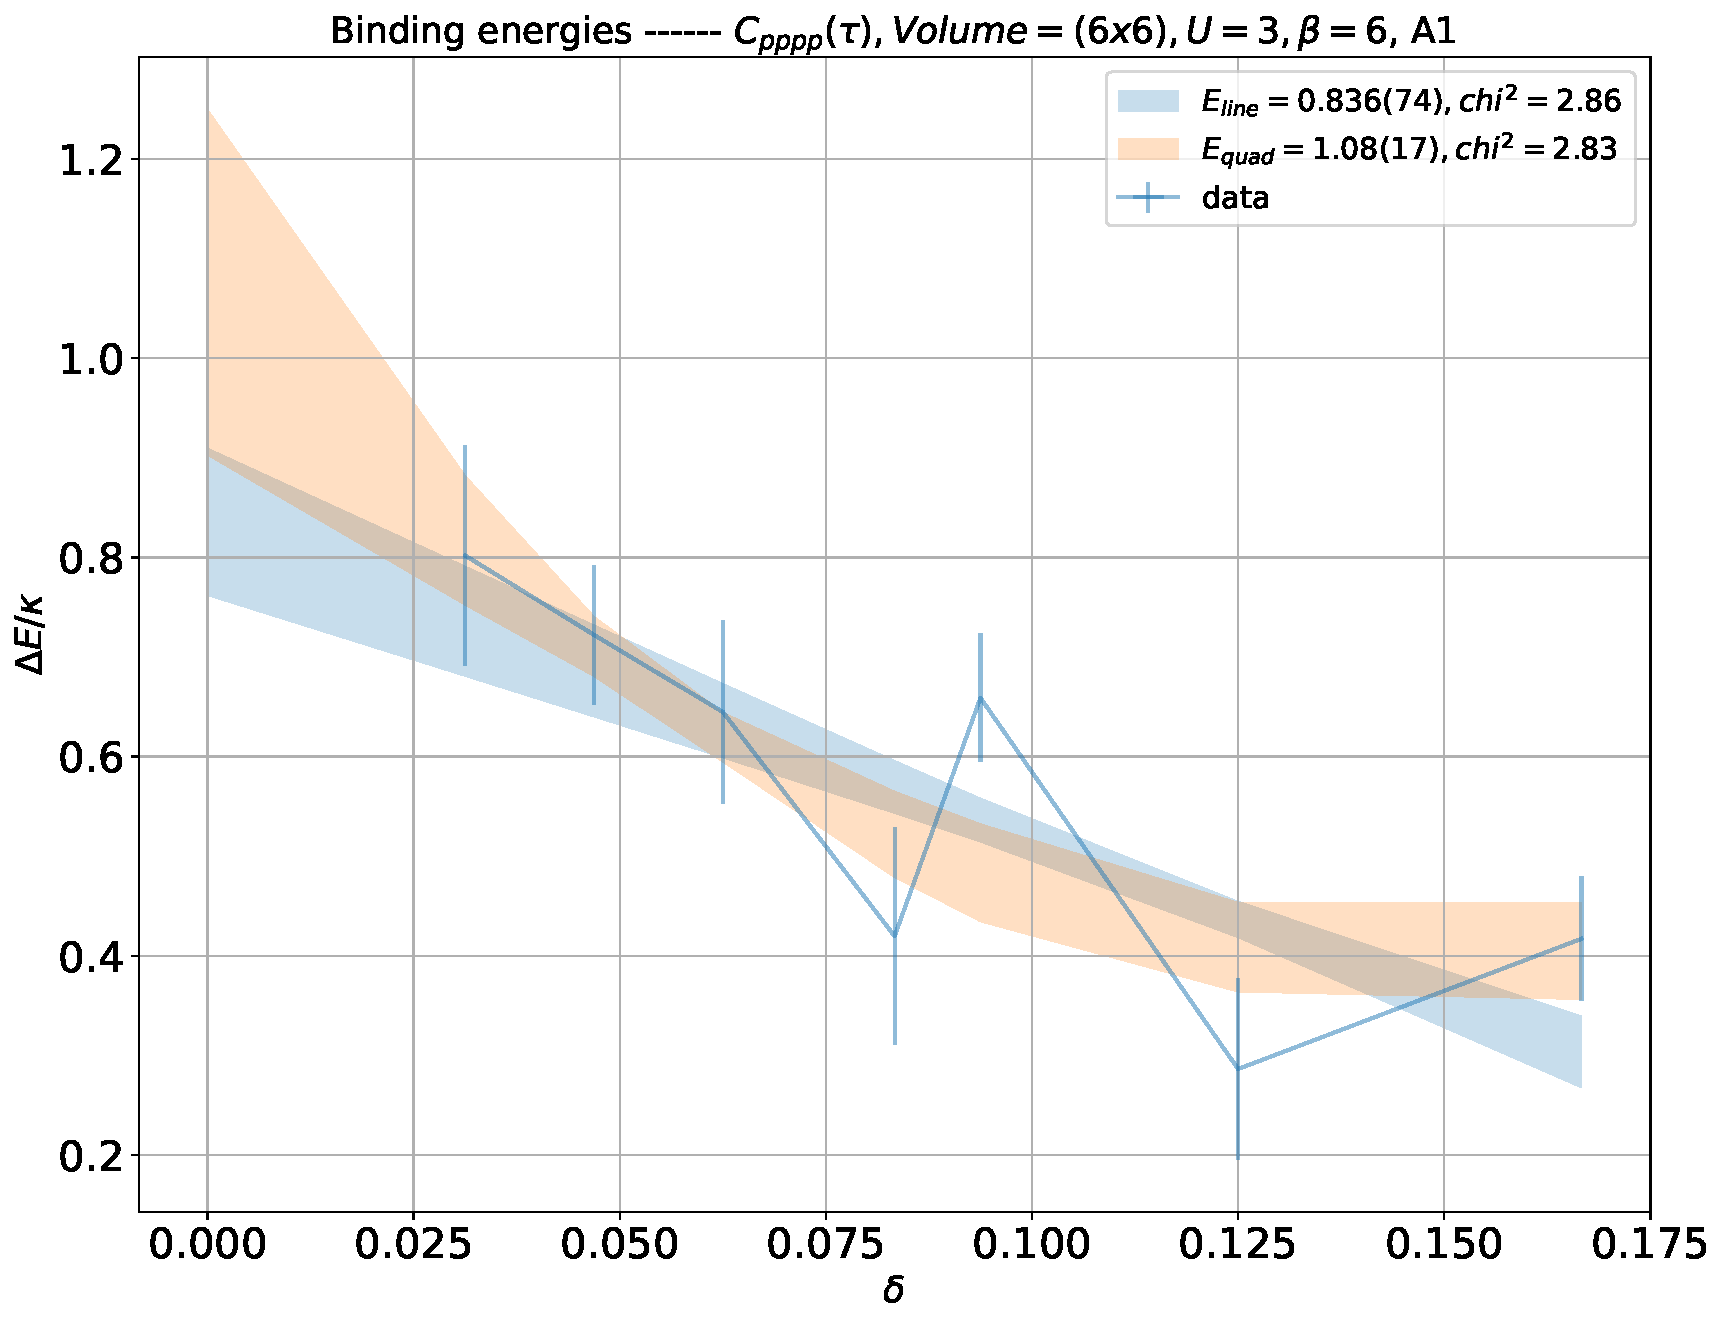
\includegraphics[width=\linewidth]{pppp-0-A1_6x6_U3.0_B6.0_cont.pdf}
  \end{subfigure}
  \begin{subfigure}{.5\textwidth}
      \centering
      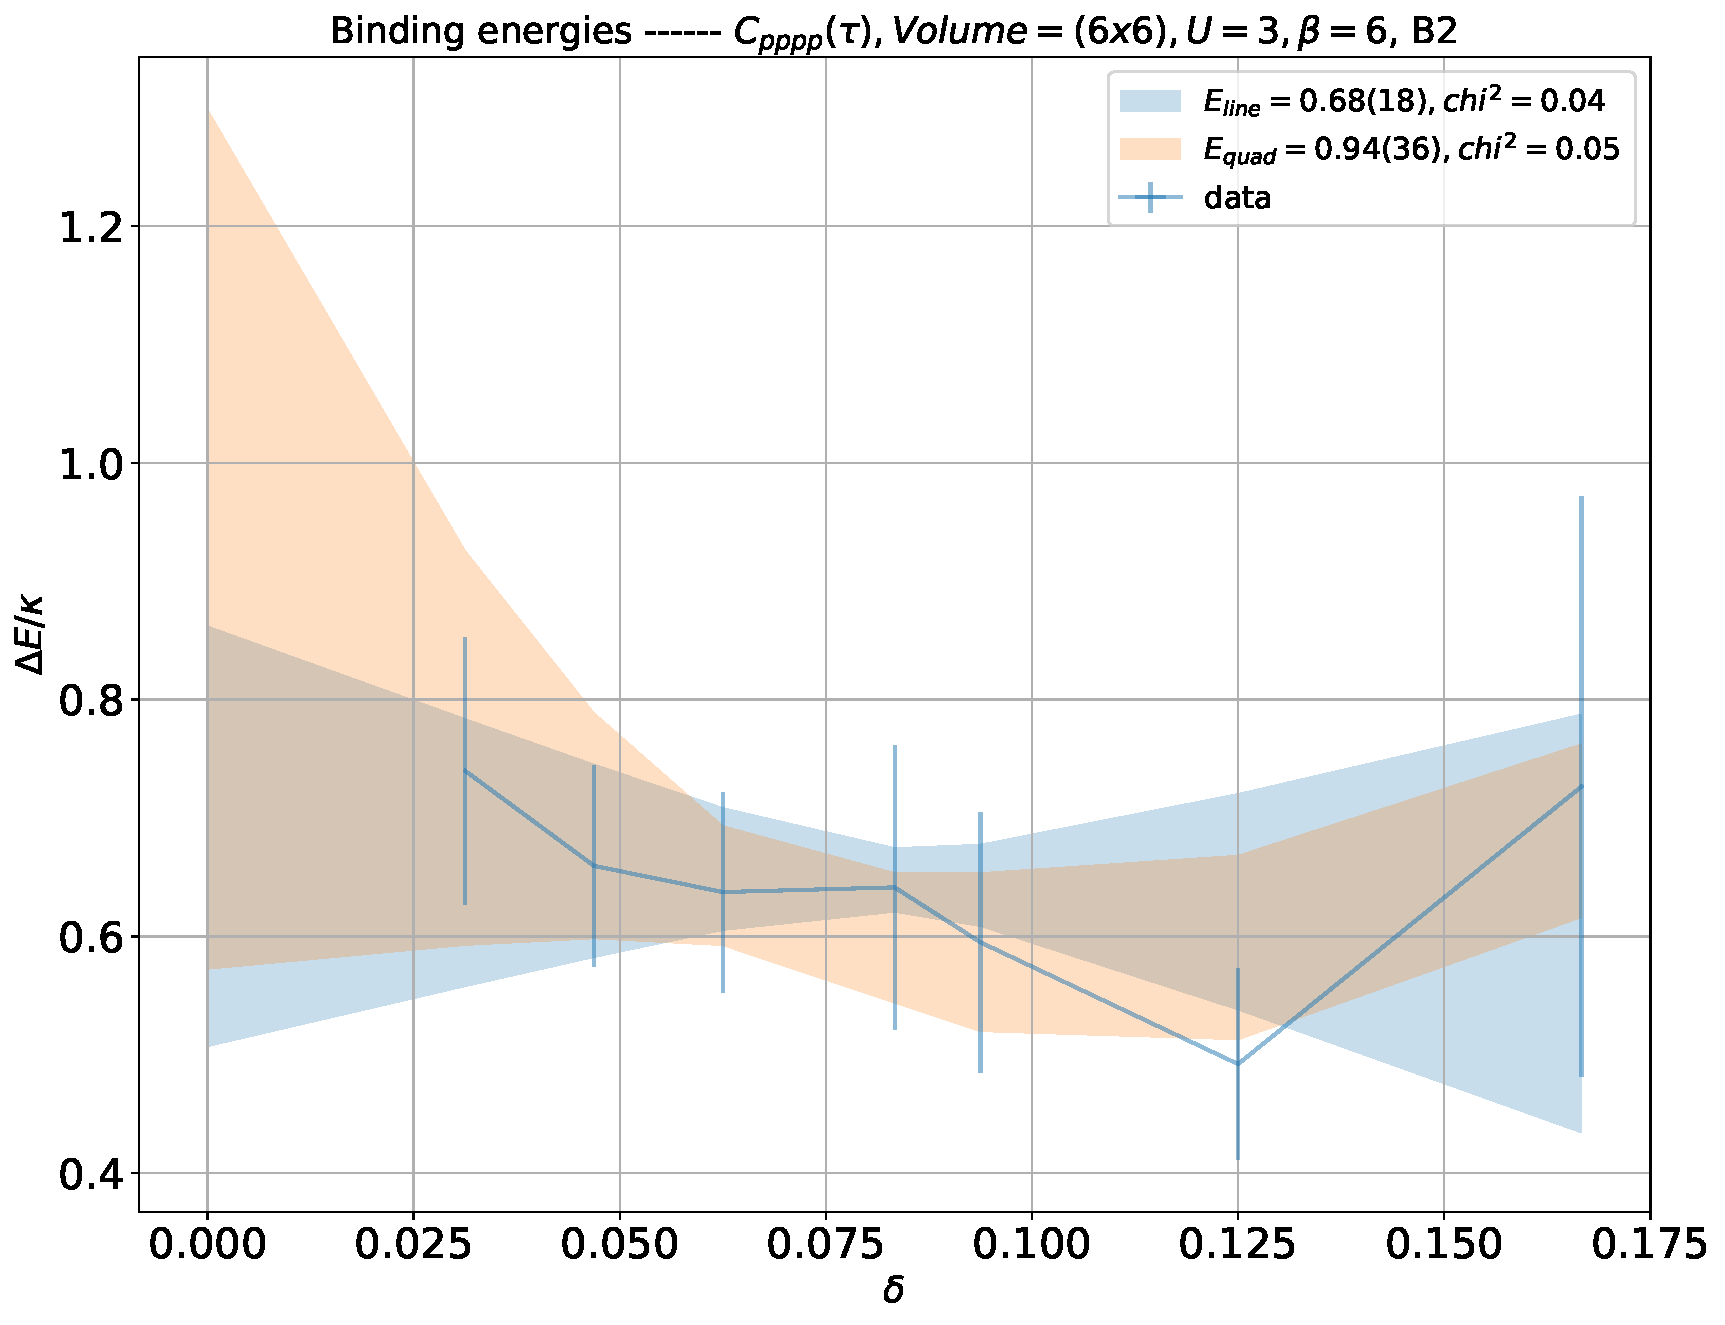
\includegraphics[width=\linewidth]{pppp-0-B2_6x6_U3.0_B6.0_cont.pdf}
  \end{subfigure}
  \caption{Binding energy extraction of the particle-particle pair at both irreducible representations, where we fit one- and two-body correlators for every $N_t$. This is followed by fitting a linear and a quadratic functions to the $\Delta E_{N_t}$ in order to extrapolate to the continuum limit ($N_t\to\infty$).}
  \label{fig:fig6}
\end{figure}

\begin{figure}
  \begin{subfigure}{.5\textwidth}
    \centering
    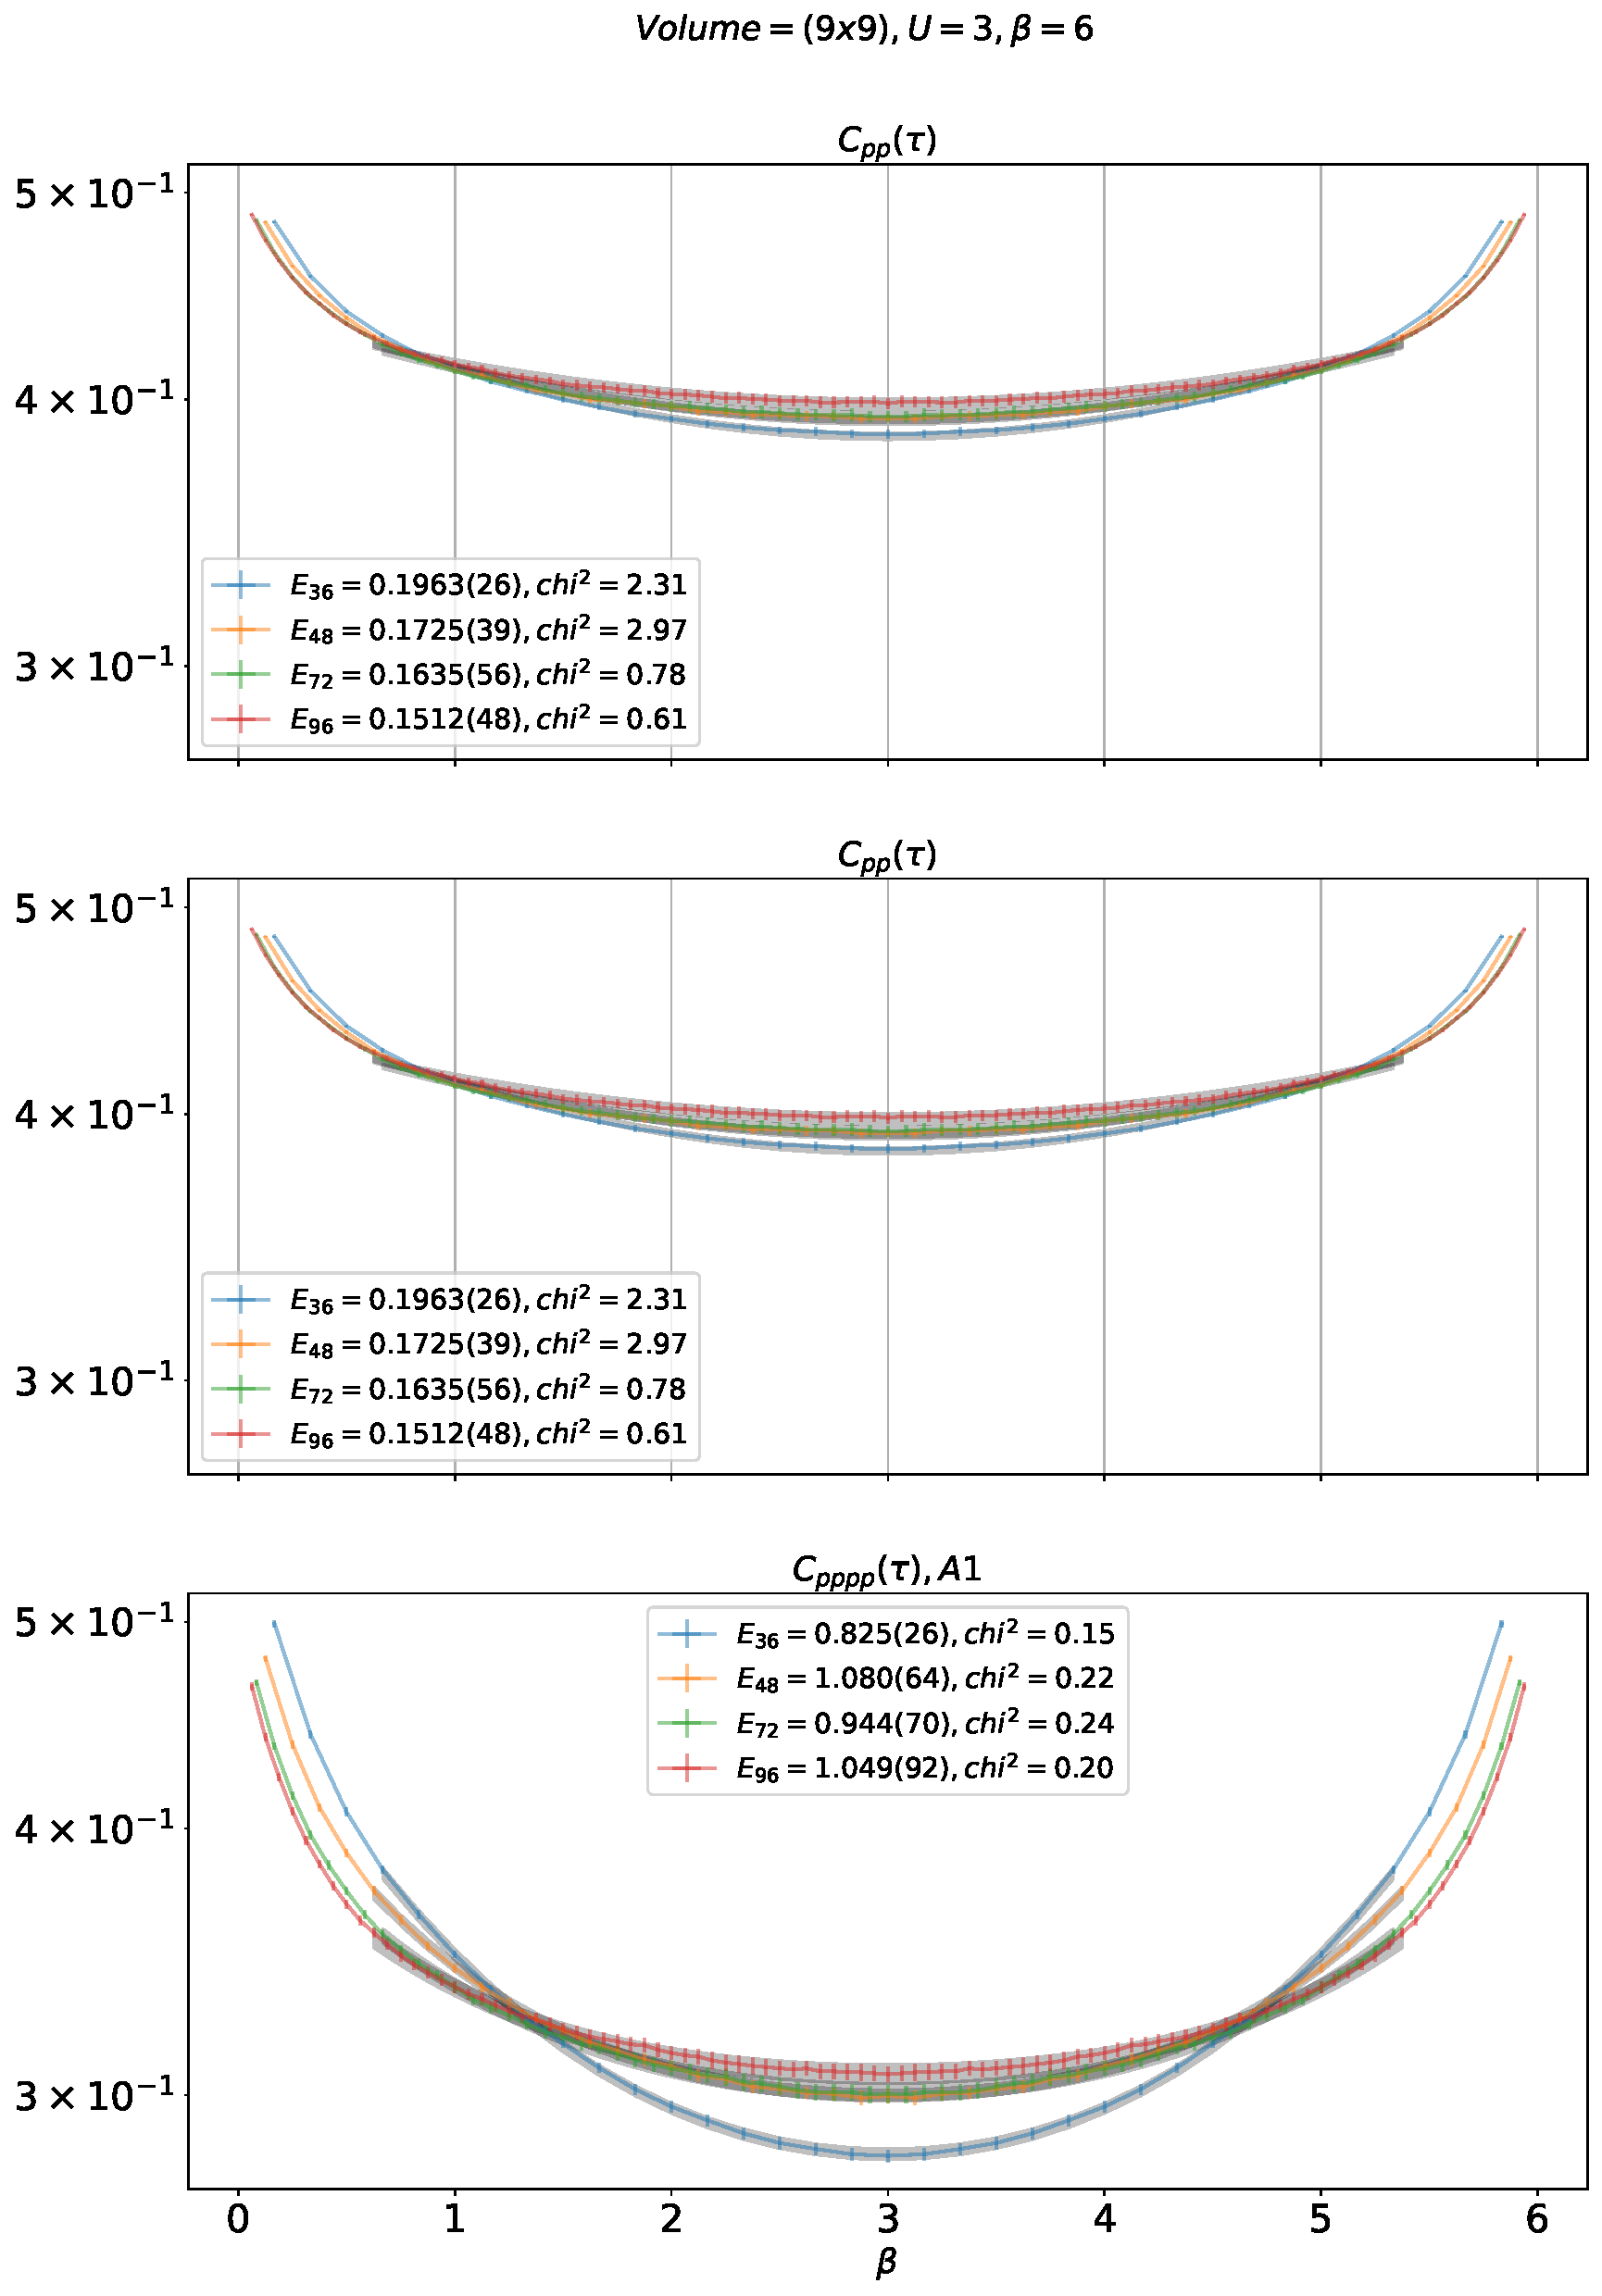
\includegraphics[width=\linewidth]{pppp-0-A1_9x9_U3_B6.pdf}
  \end{subfigure}%
  \begin{subfigure}{.5\textwidth}
    \centering
    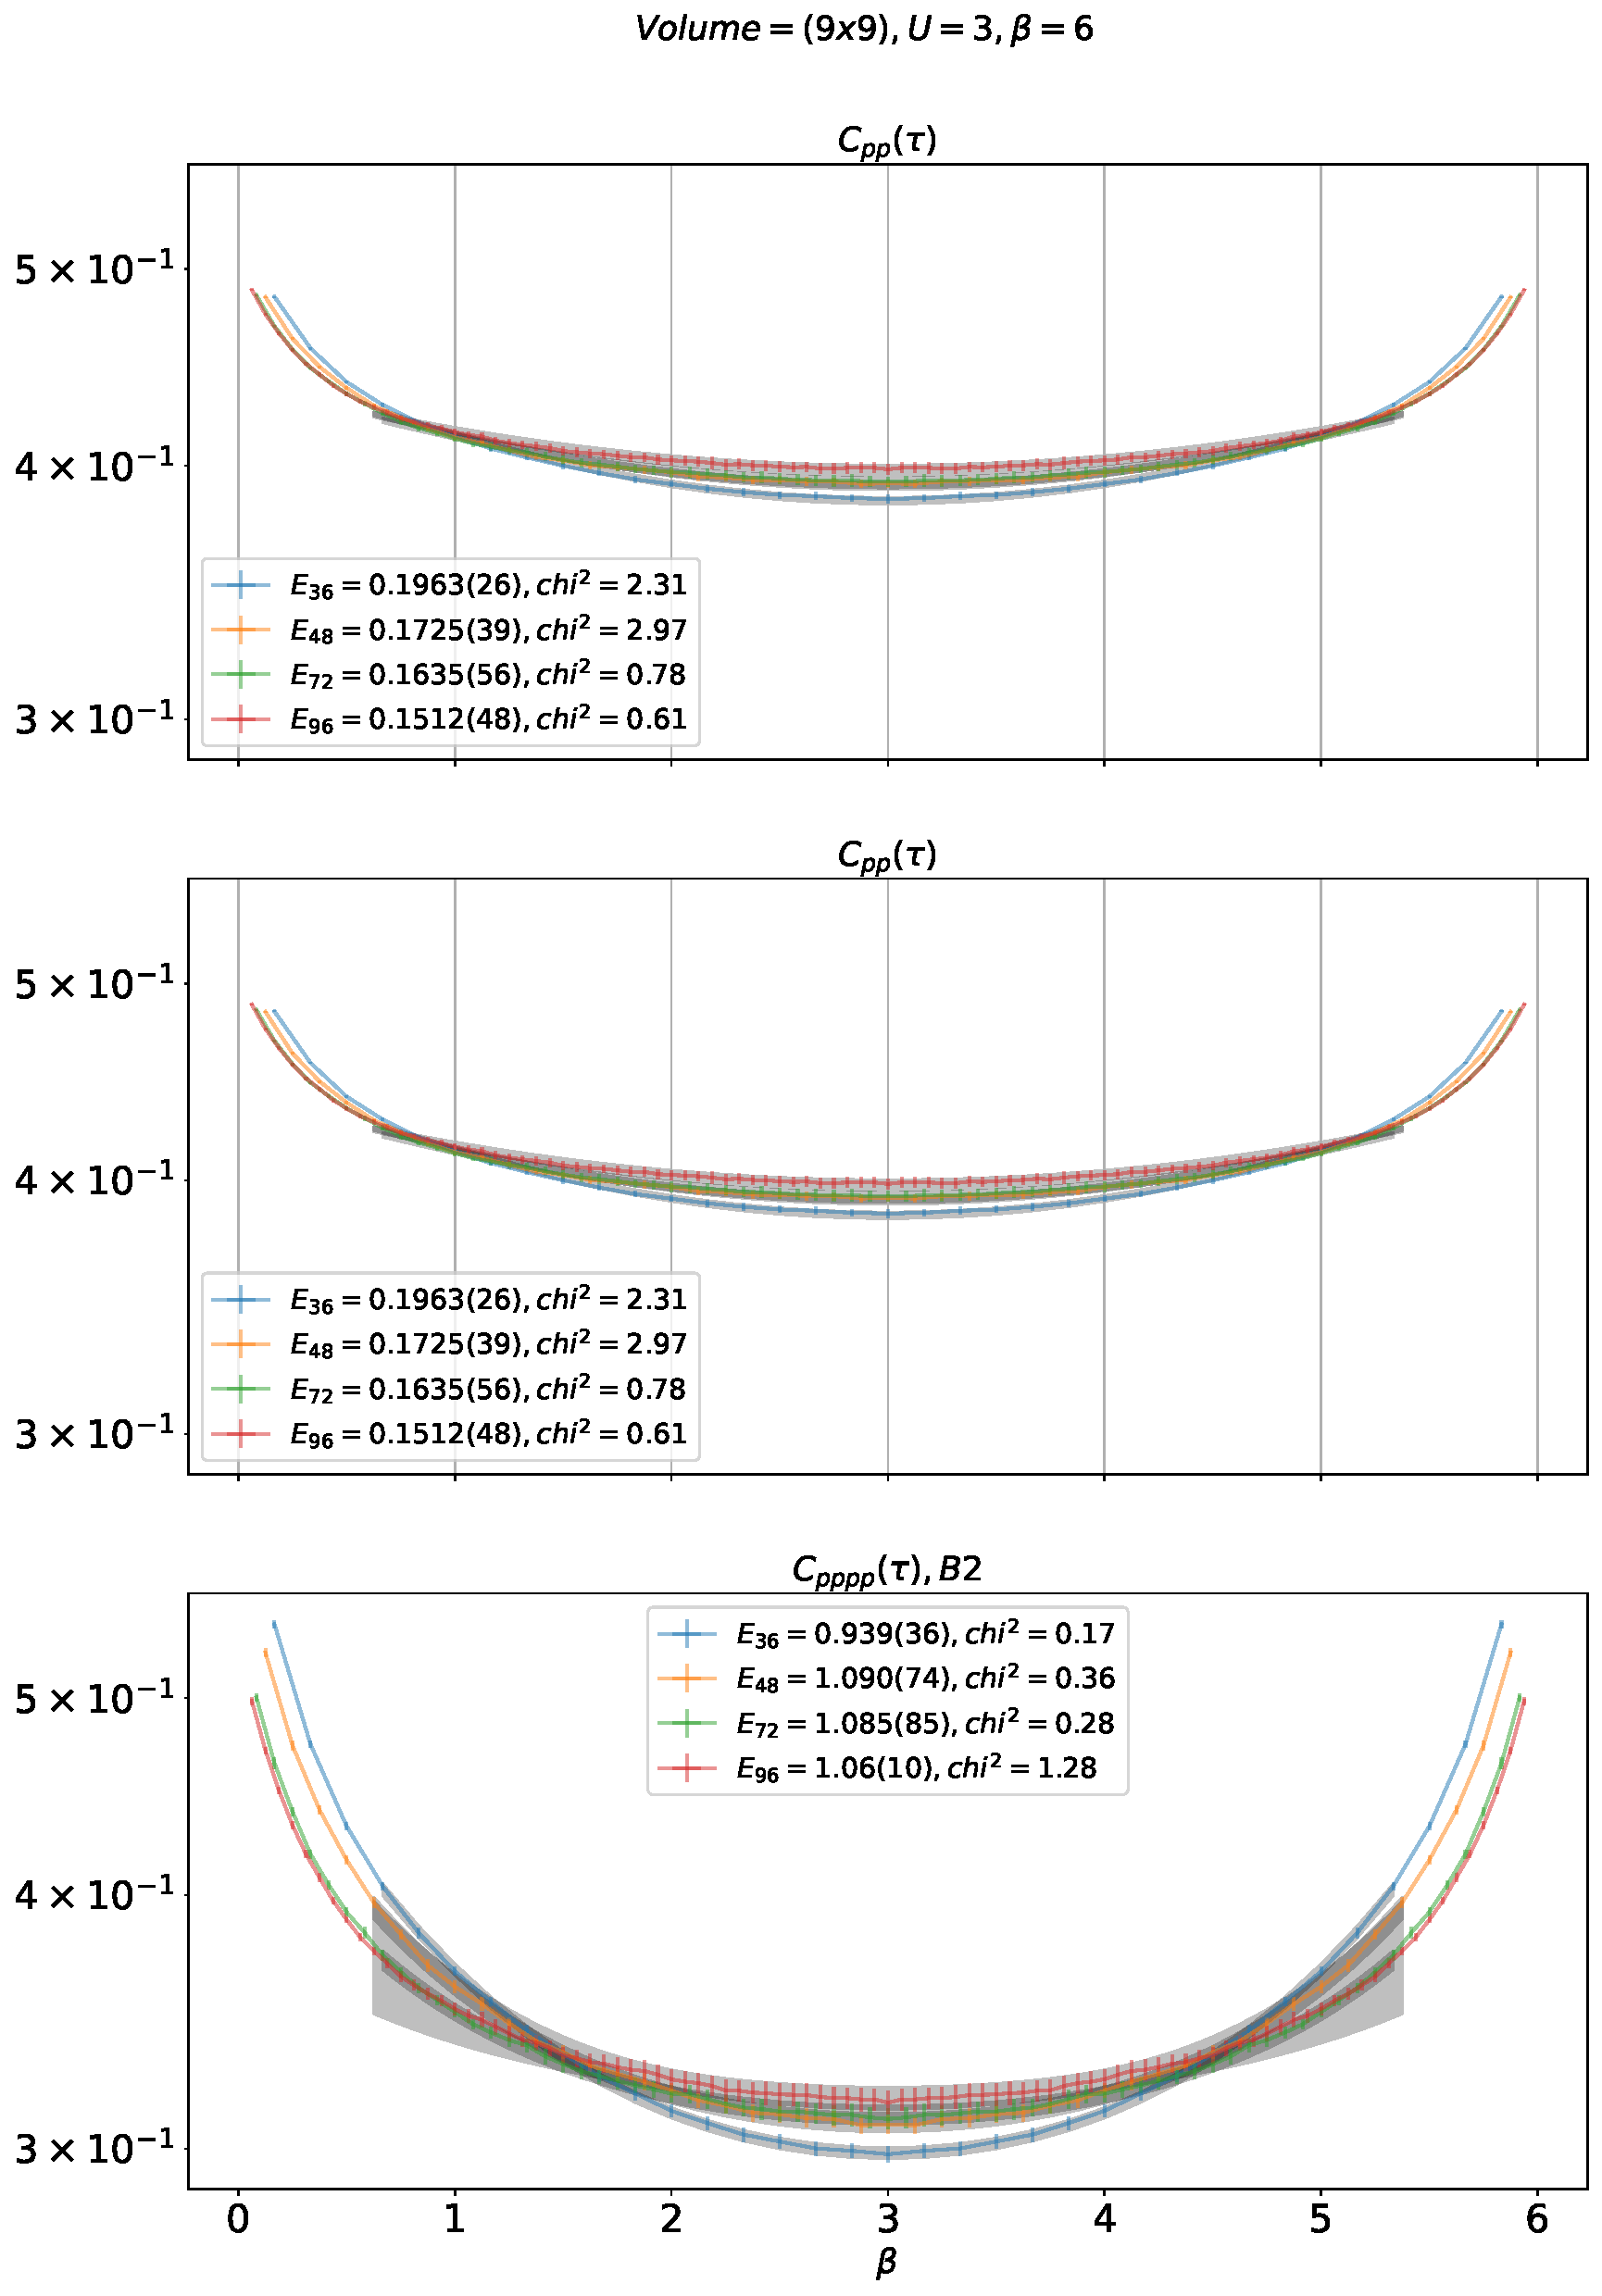
\includegraphics[width=\linewidth]{pppp-0-B2_9x9_U3_B6.pdf}
  \end{subfigure}
  \begin{subfigure}{.5\textwidth}
      \centering
      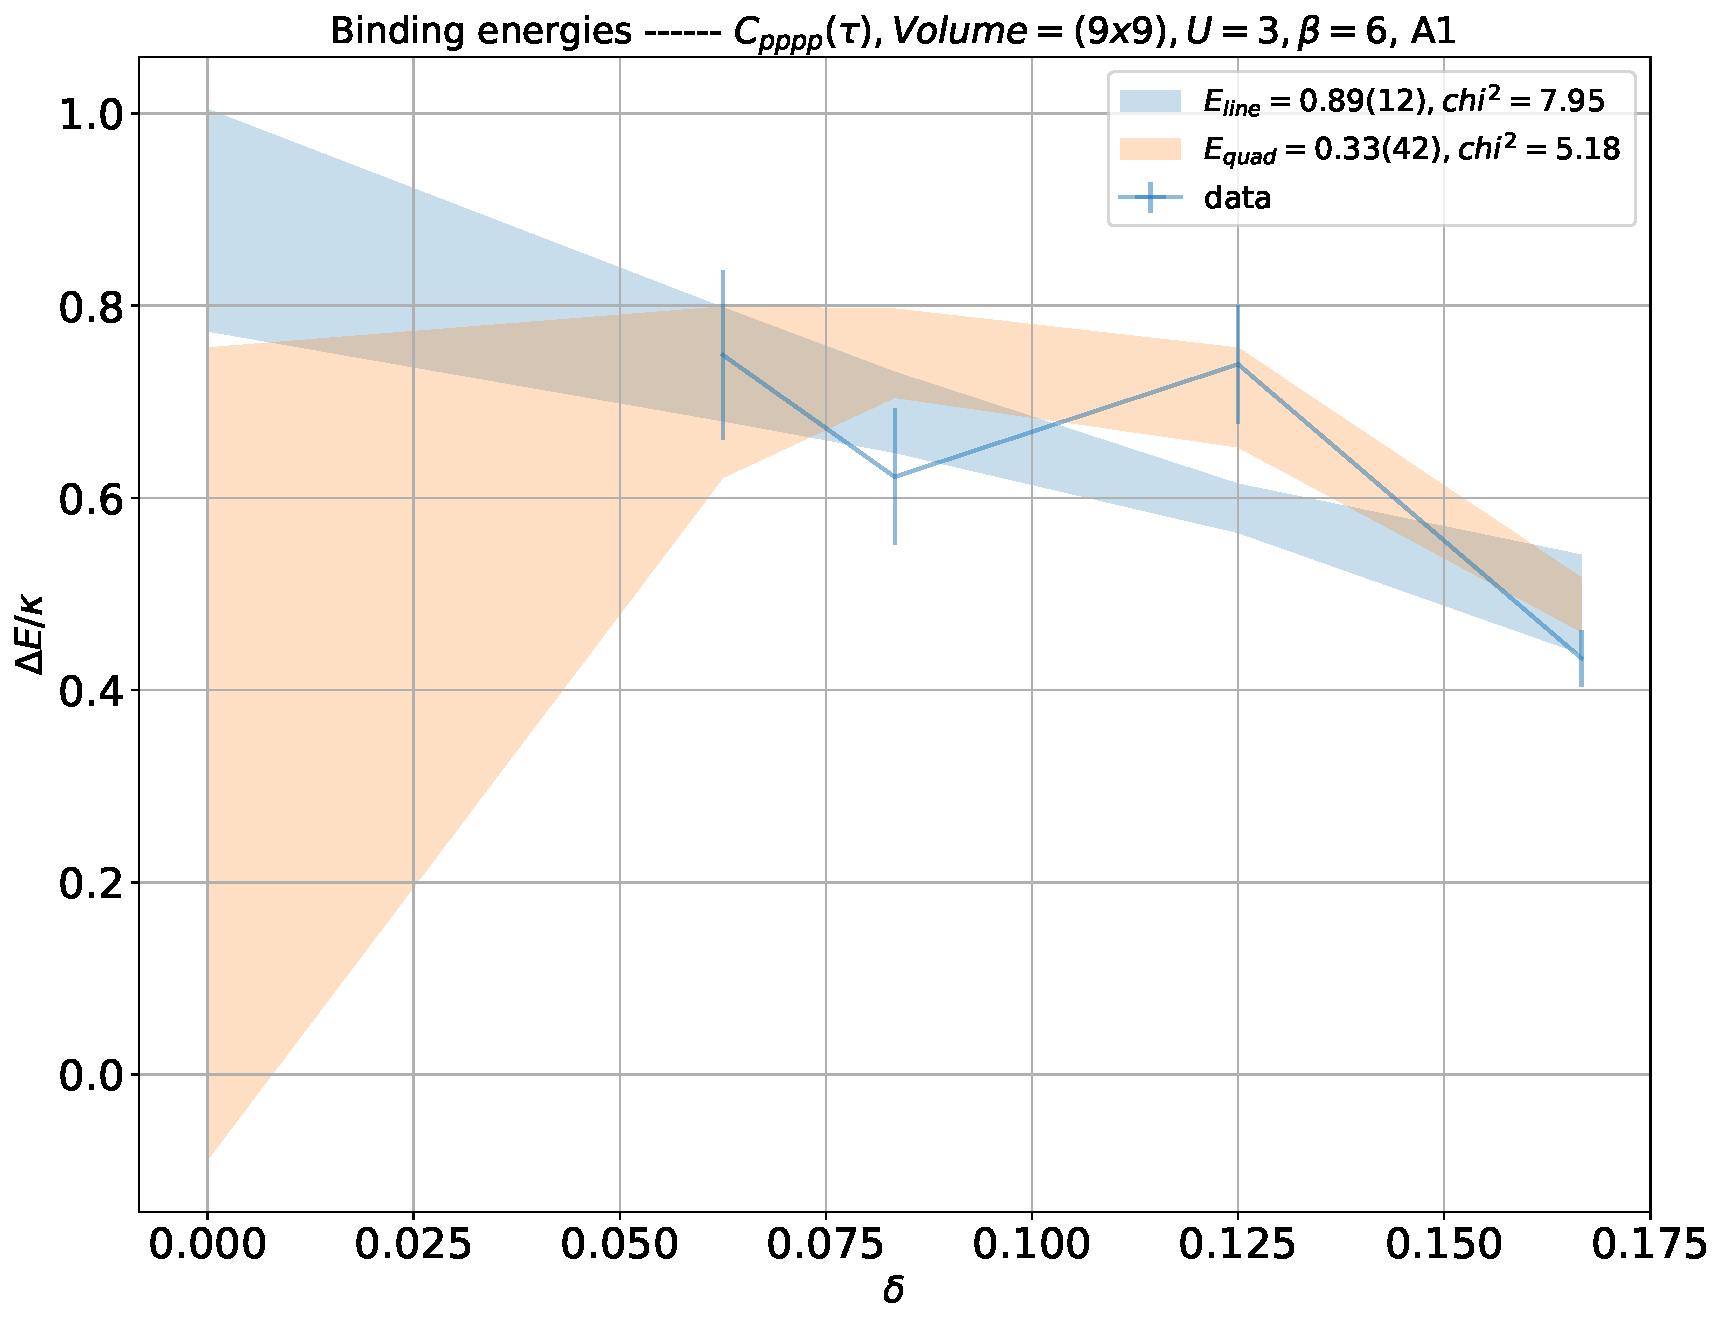
\includegraphics[width=\linewidth]{pppp-0-A1_9x9_U3_B6_cont.pdf}
  \end{subfigure}
  \begin{subfigure}{.5\textwidth}
      \centering
      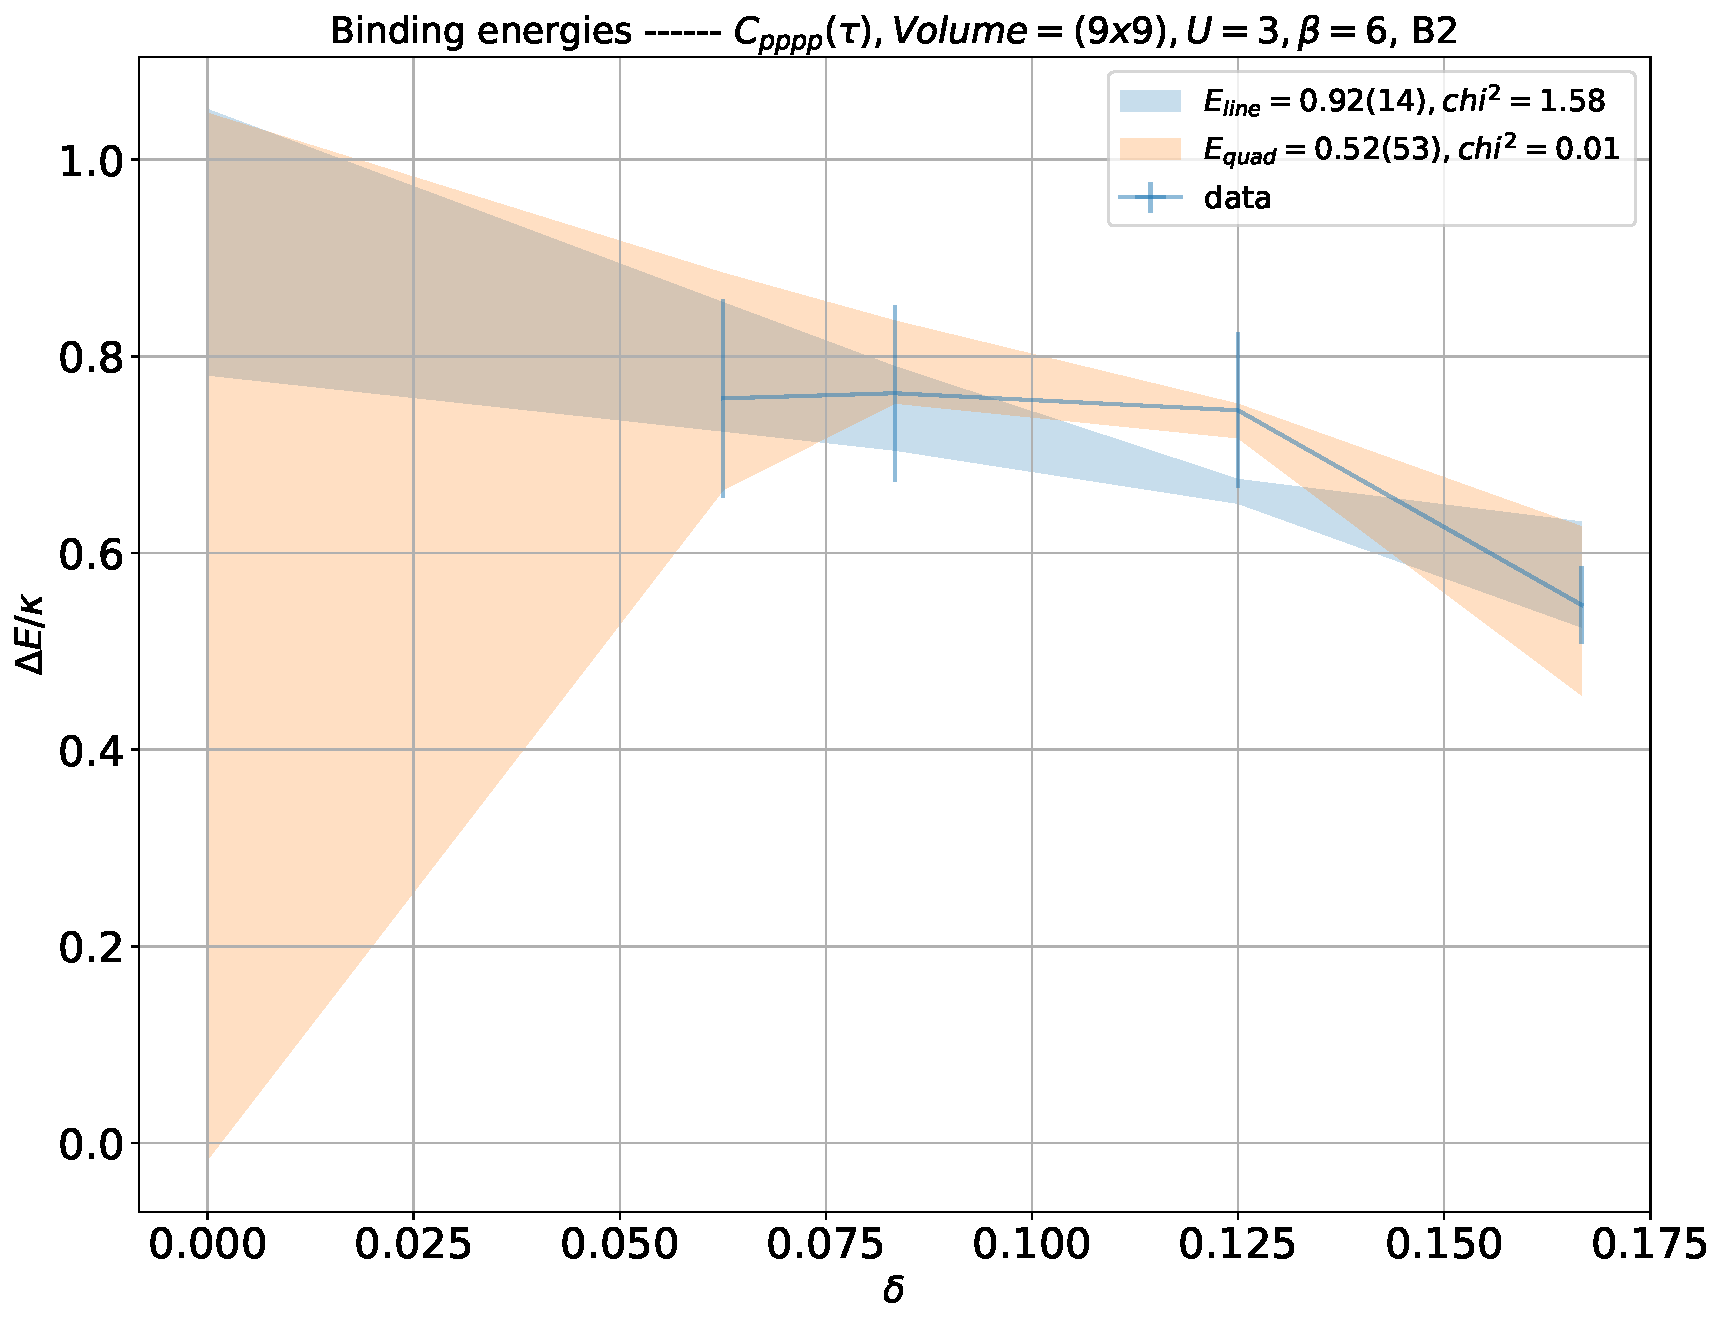
\includegraphics[width=\linewidth]{pppp-0-B2_9x9_U3_B6_cont.pdf}
  \end{subfigure}
  \caption{Binding energy extraction of the particle-particle pair at both irreducible representations, where we fit one- and two-body correlators for every $N_t$. This is followed by fitting a linear and a quadratic functions to the $\Delta E_{N_t}$ in order to extrapolate to the continuum limit ($N_t\to\infty$).}
  \label{fig:fig7}
\end{figure}

\begin{figure}
  \begin{subfigure}{.5\textwidth}
    \centering
    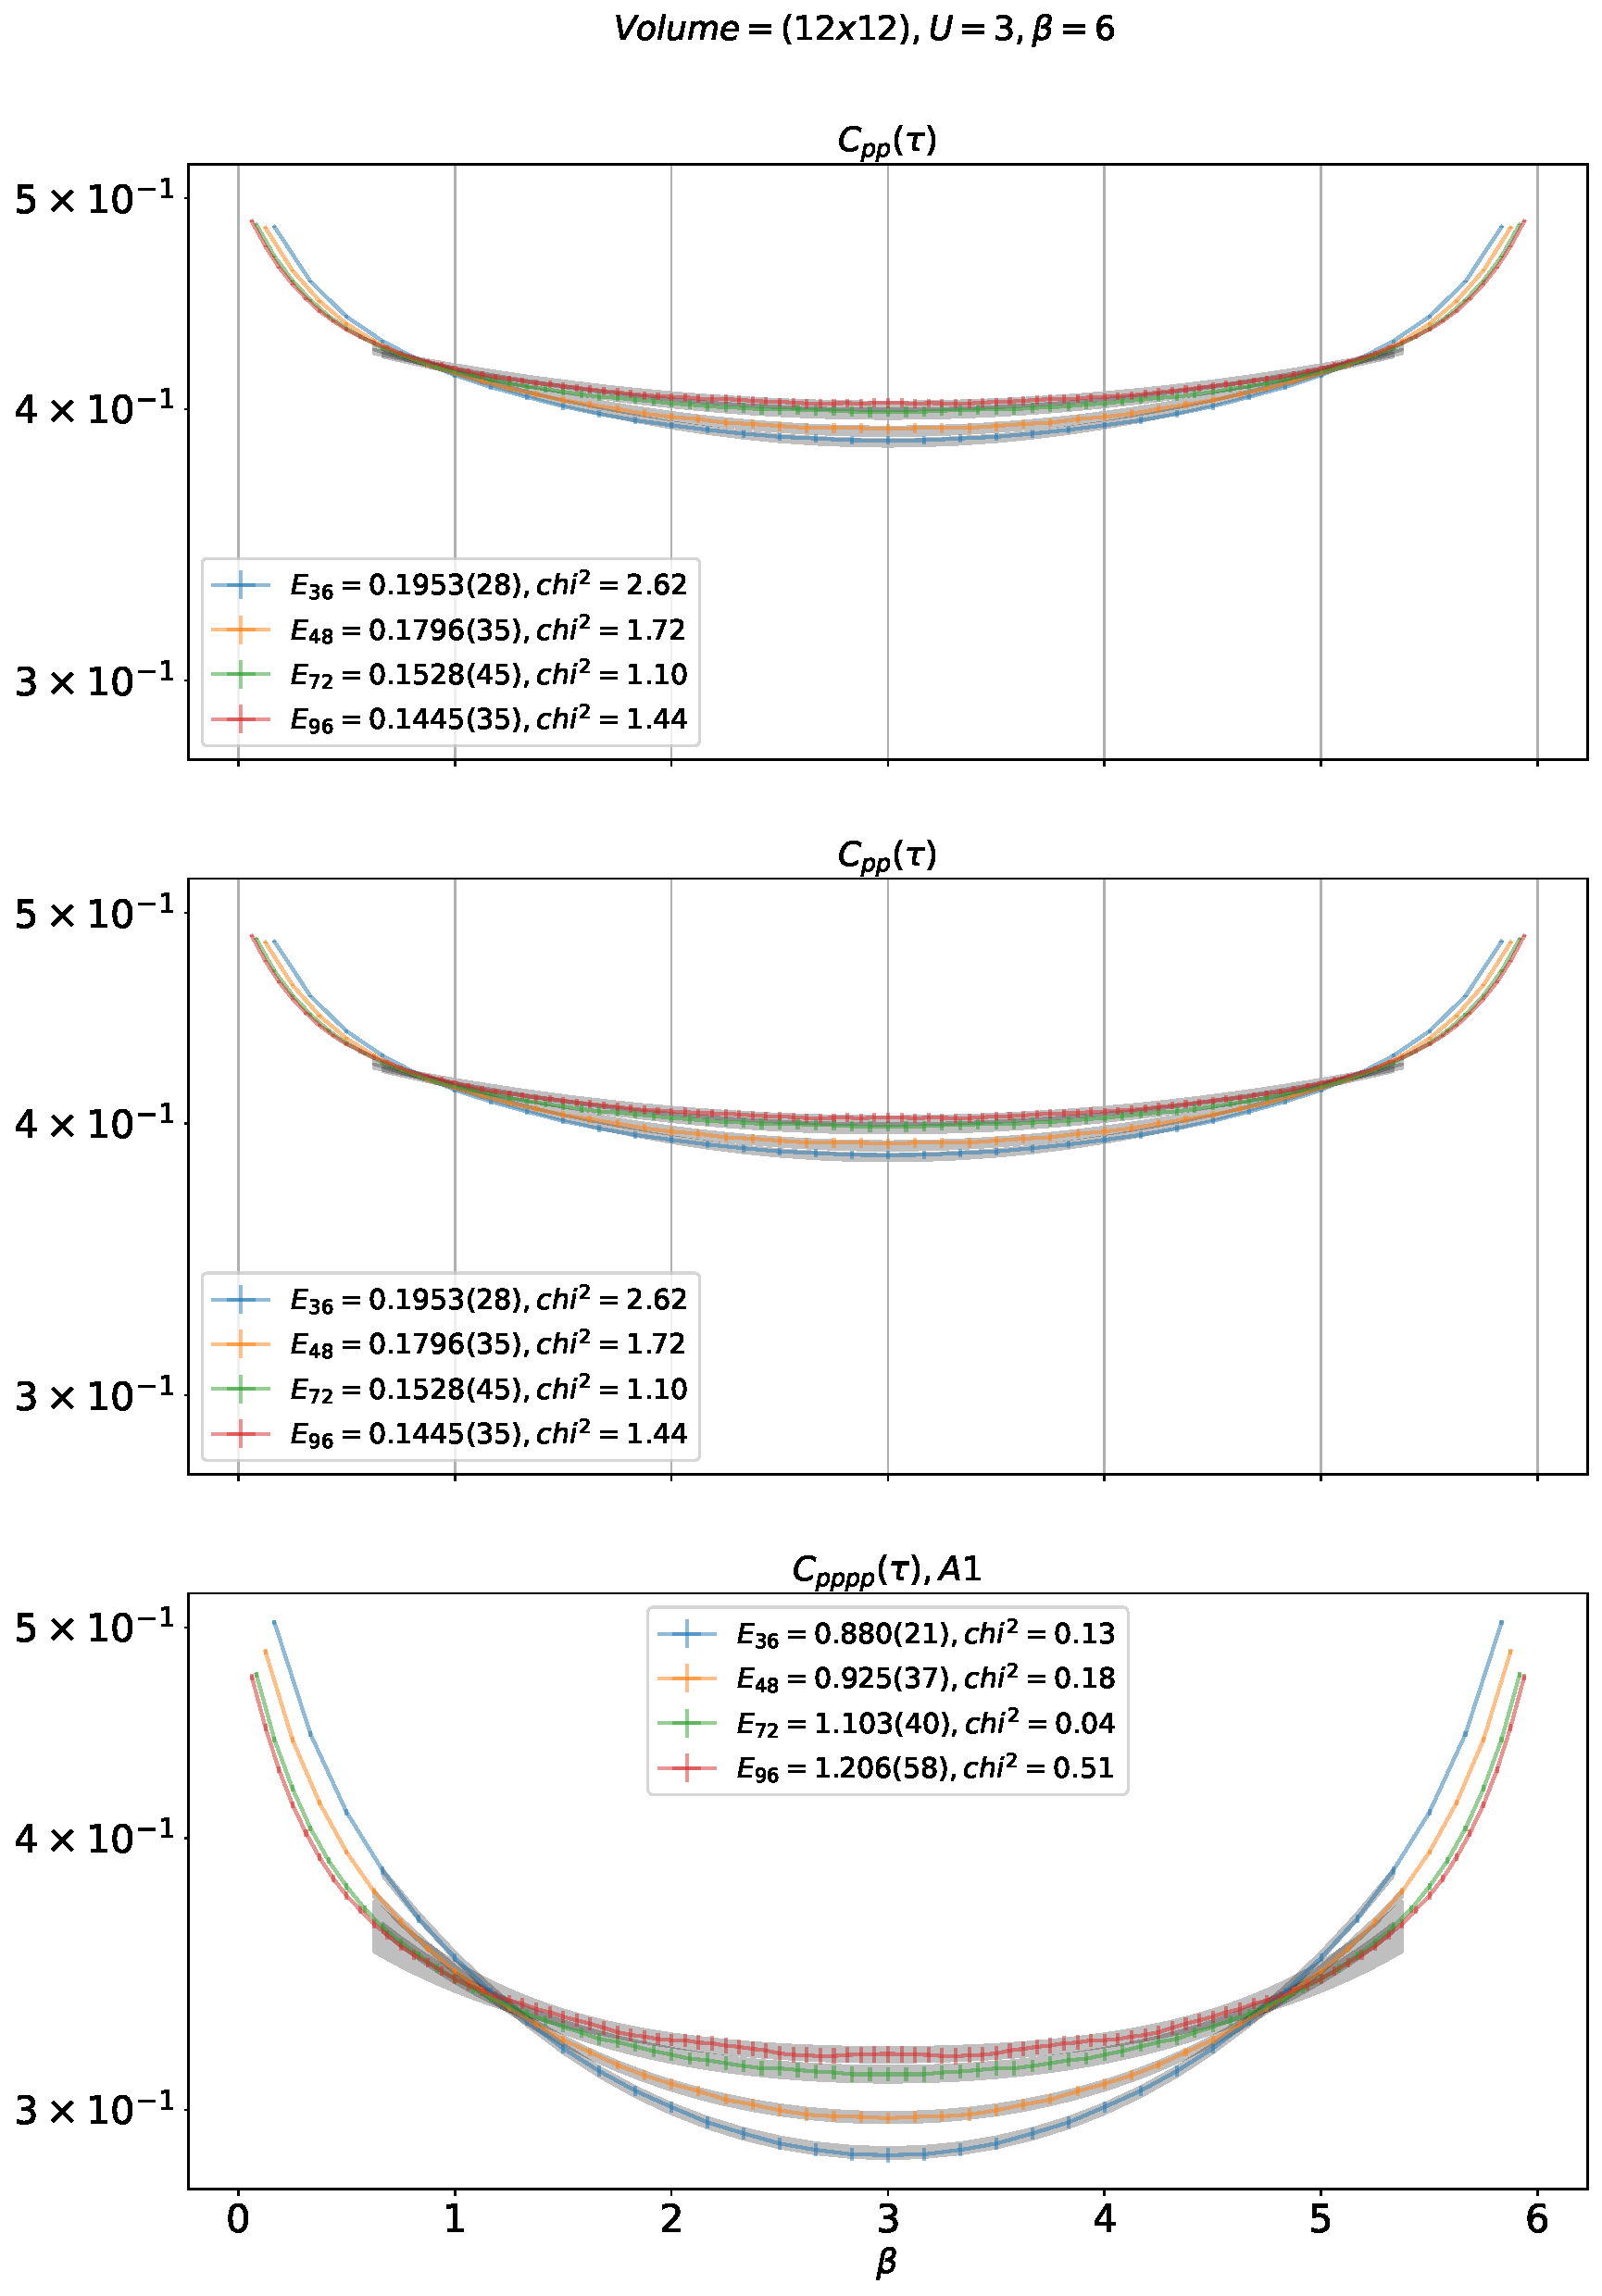
\includegraphics[width=\linewidth]{pppp-0-A1_12x12_U3_B6.pdf}
  \end{subfigure}%
  \begin{subfigure}{.5\textwidth}
    \centering
    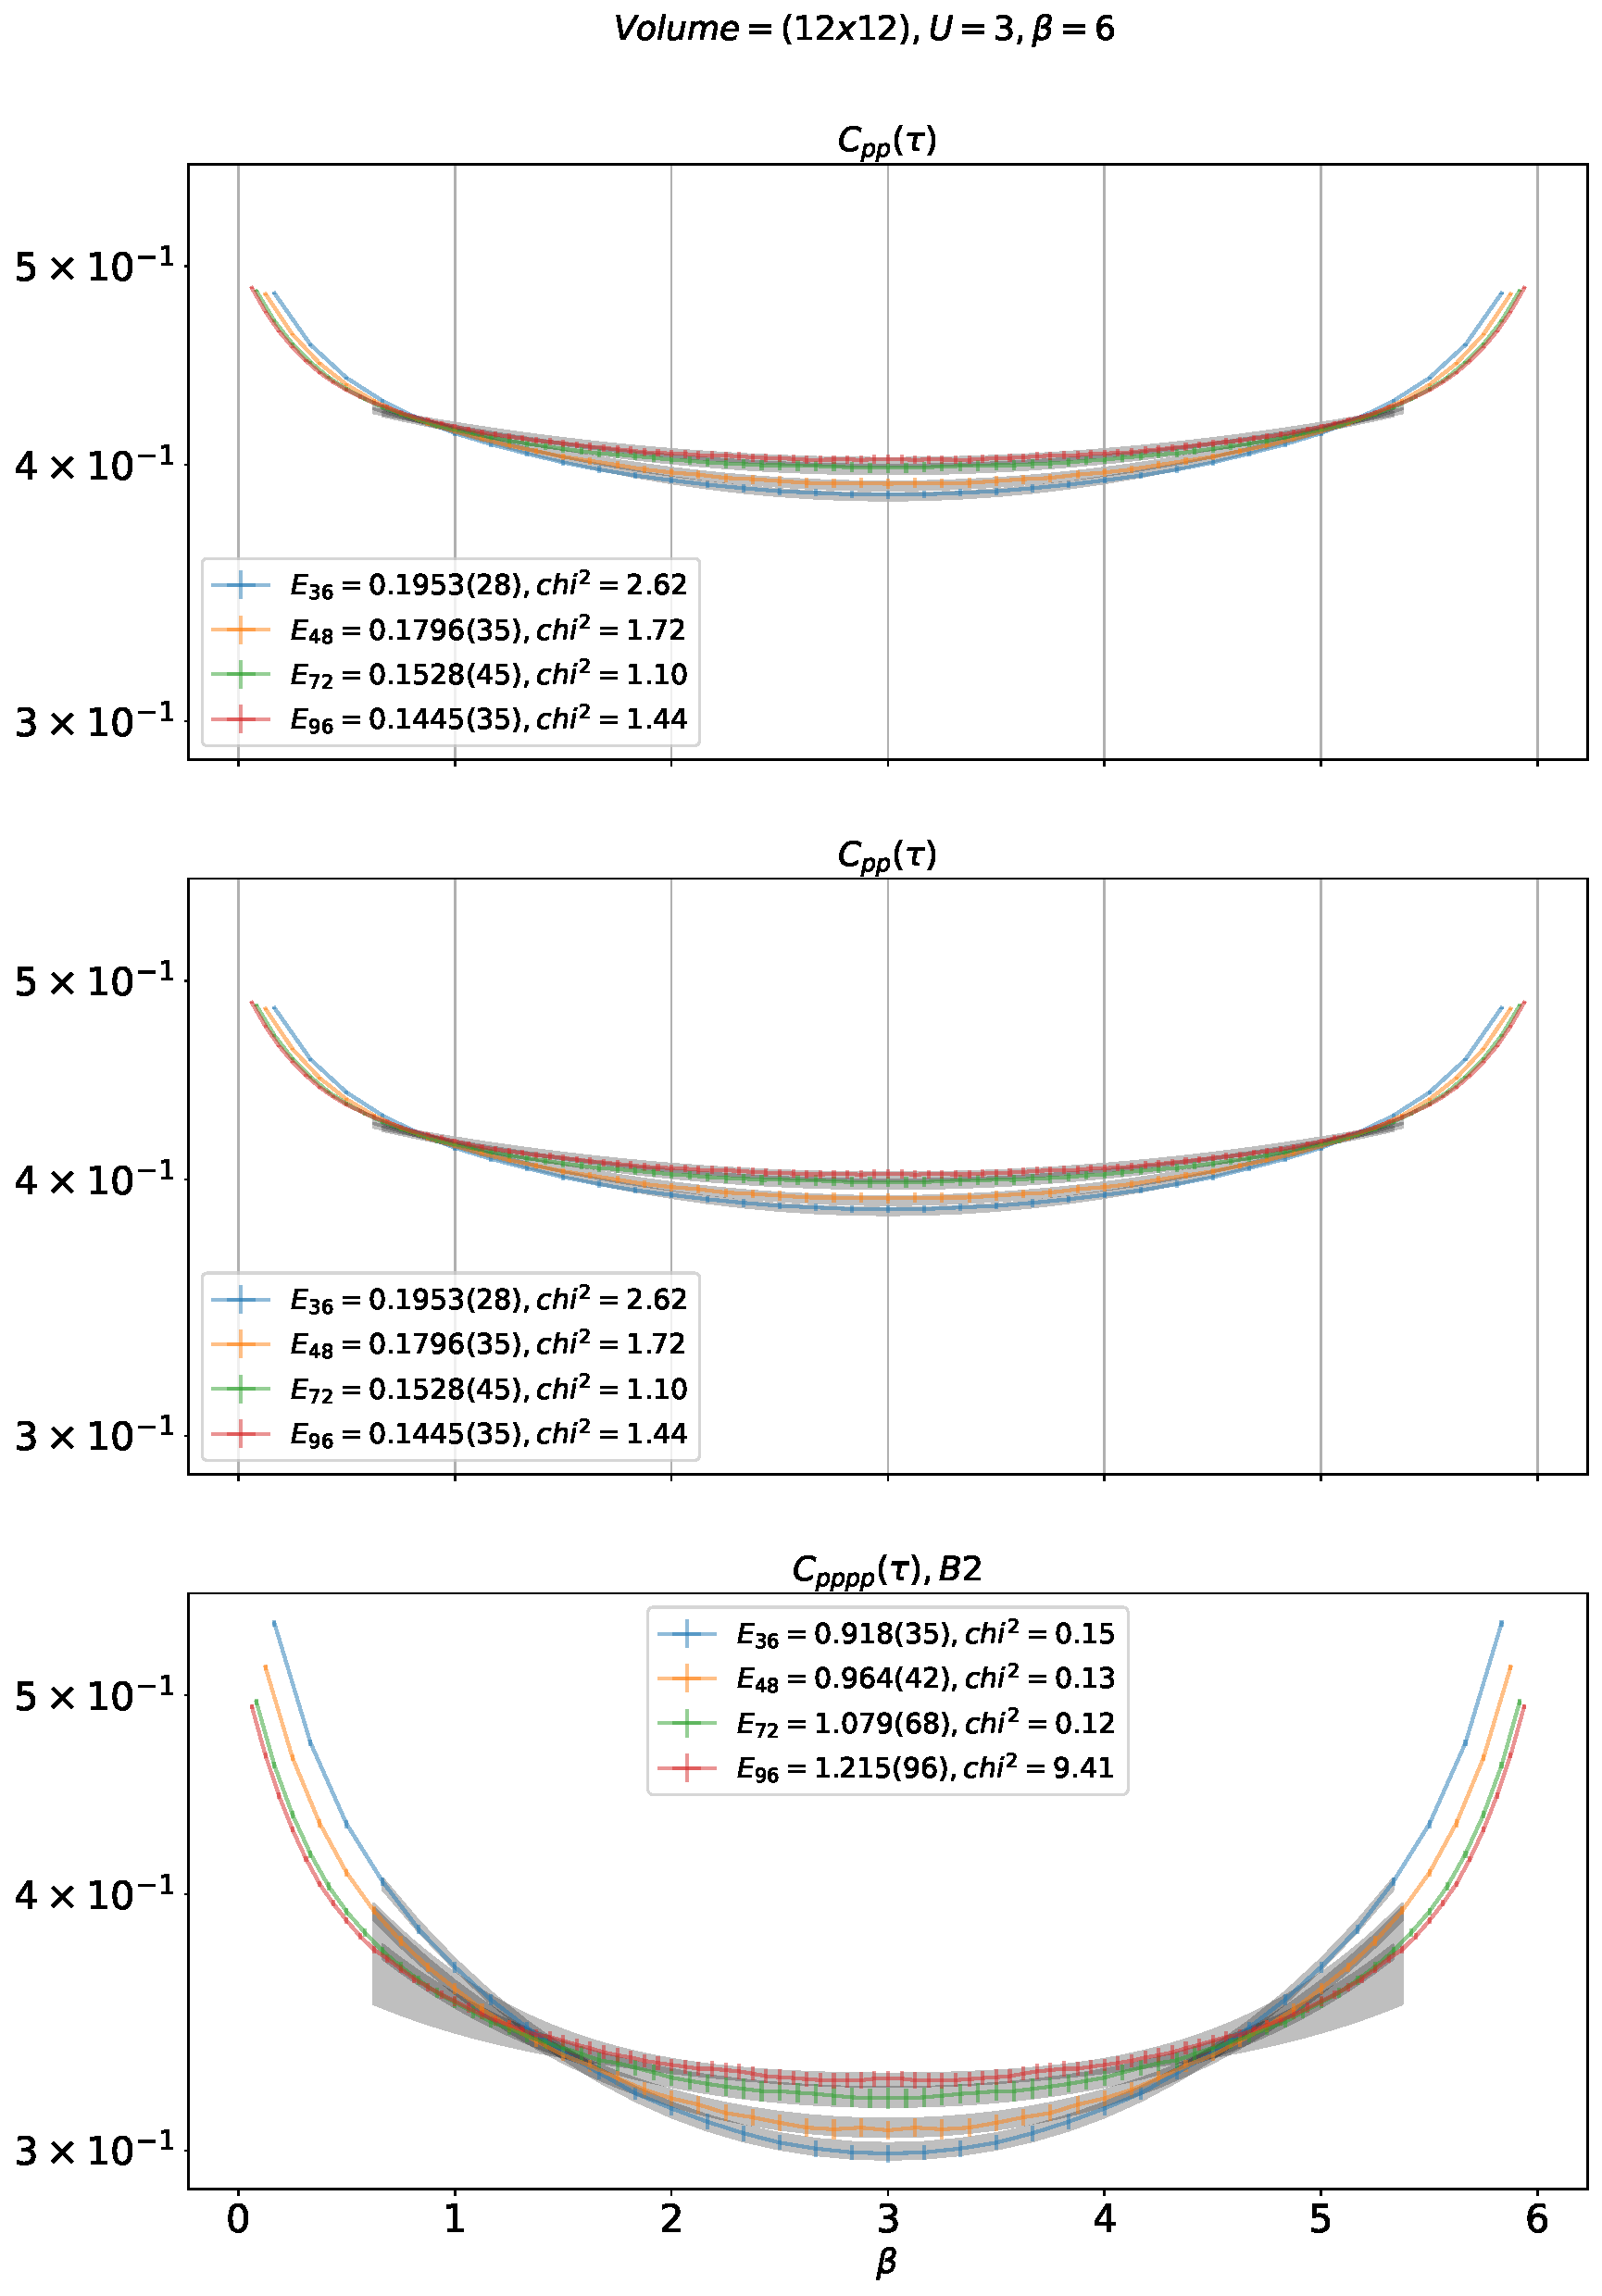
\includegraphics[width=\linewidth]{pppp-0-B2_12x12_U3_B6.pdf}
  \end{subfigure}
  \begin{subfigure}{.5\textwidth}
      \centering
      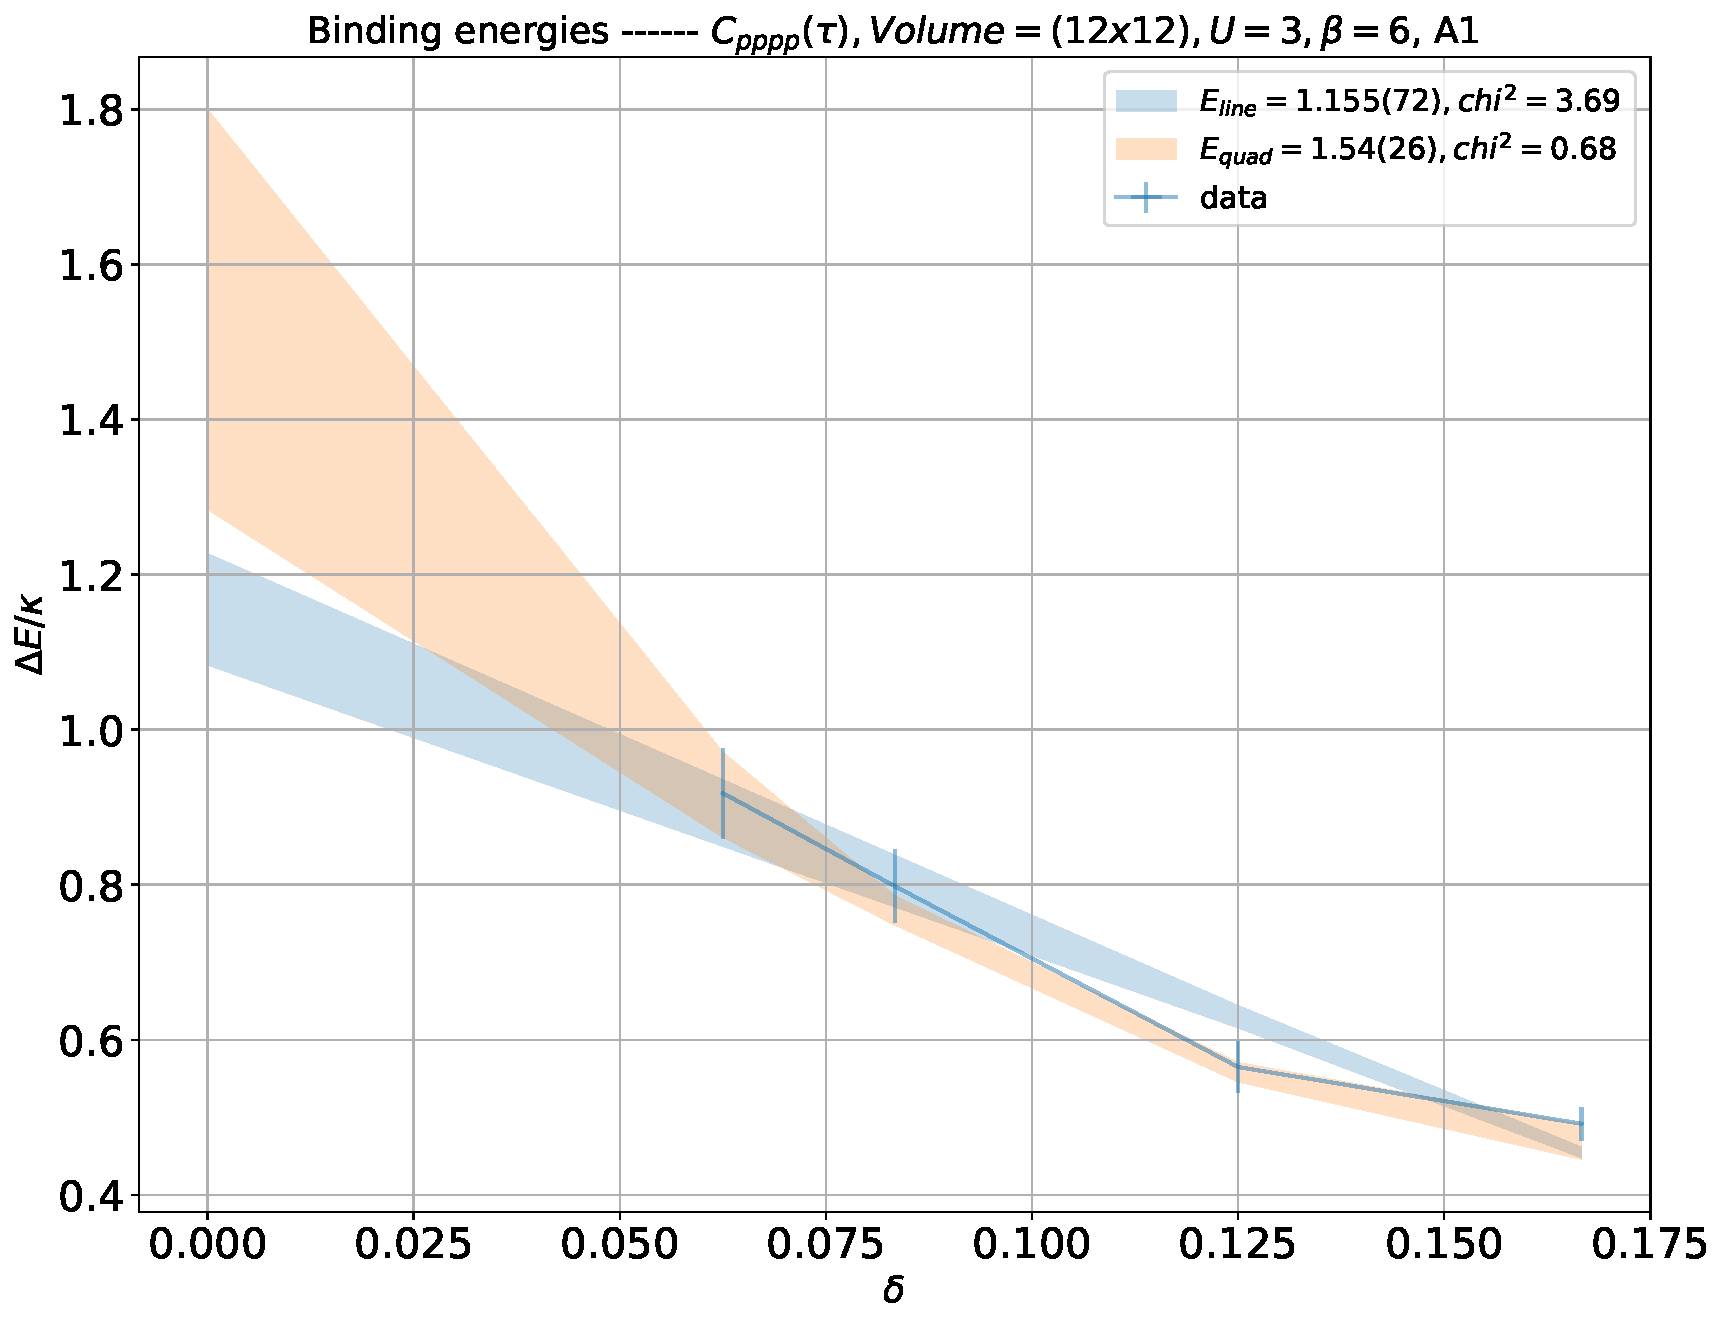
\includegraphics[width=\linewidth]{pppp-0-A1_12x12_U3_B6_cont.pdf}
  \end{subfigure}
  \begin{subfigure}{.5\textwidth}
      \centering
      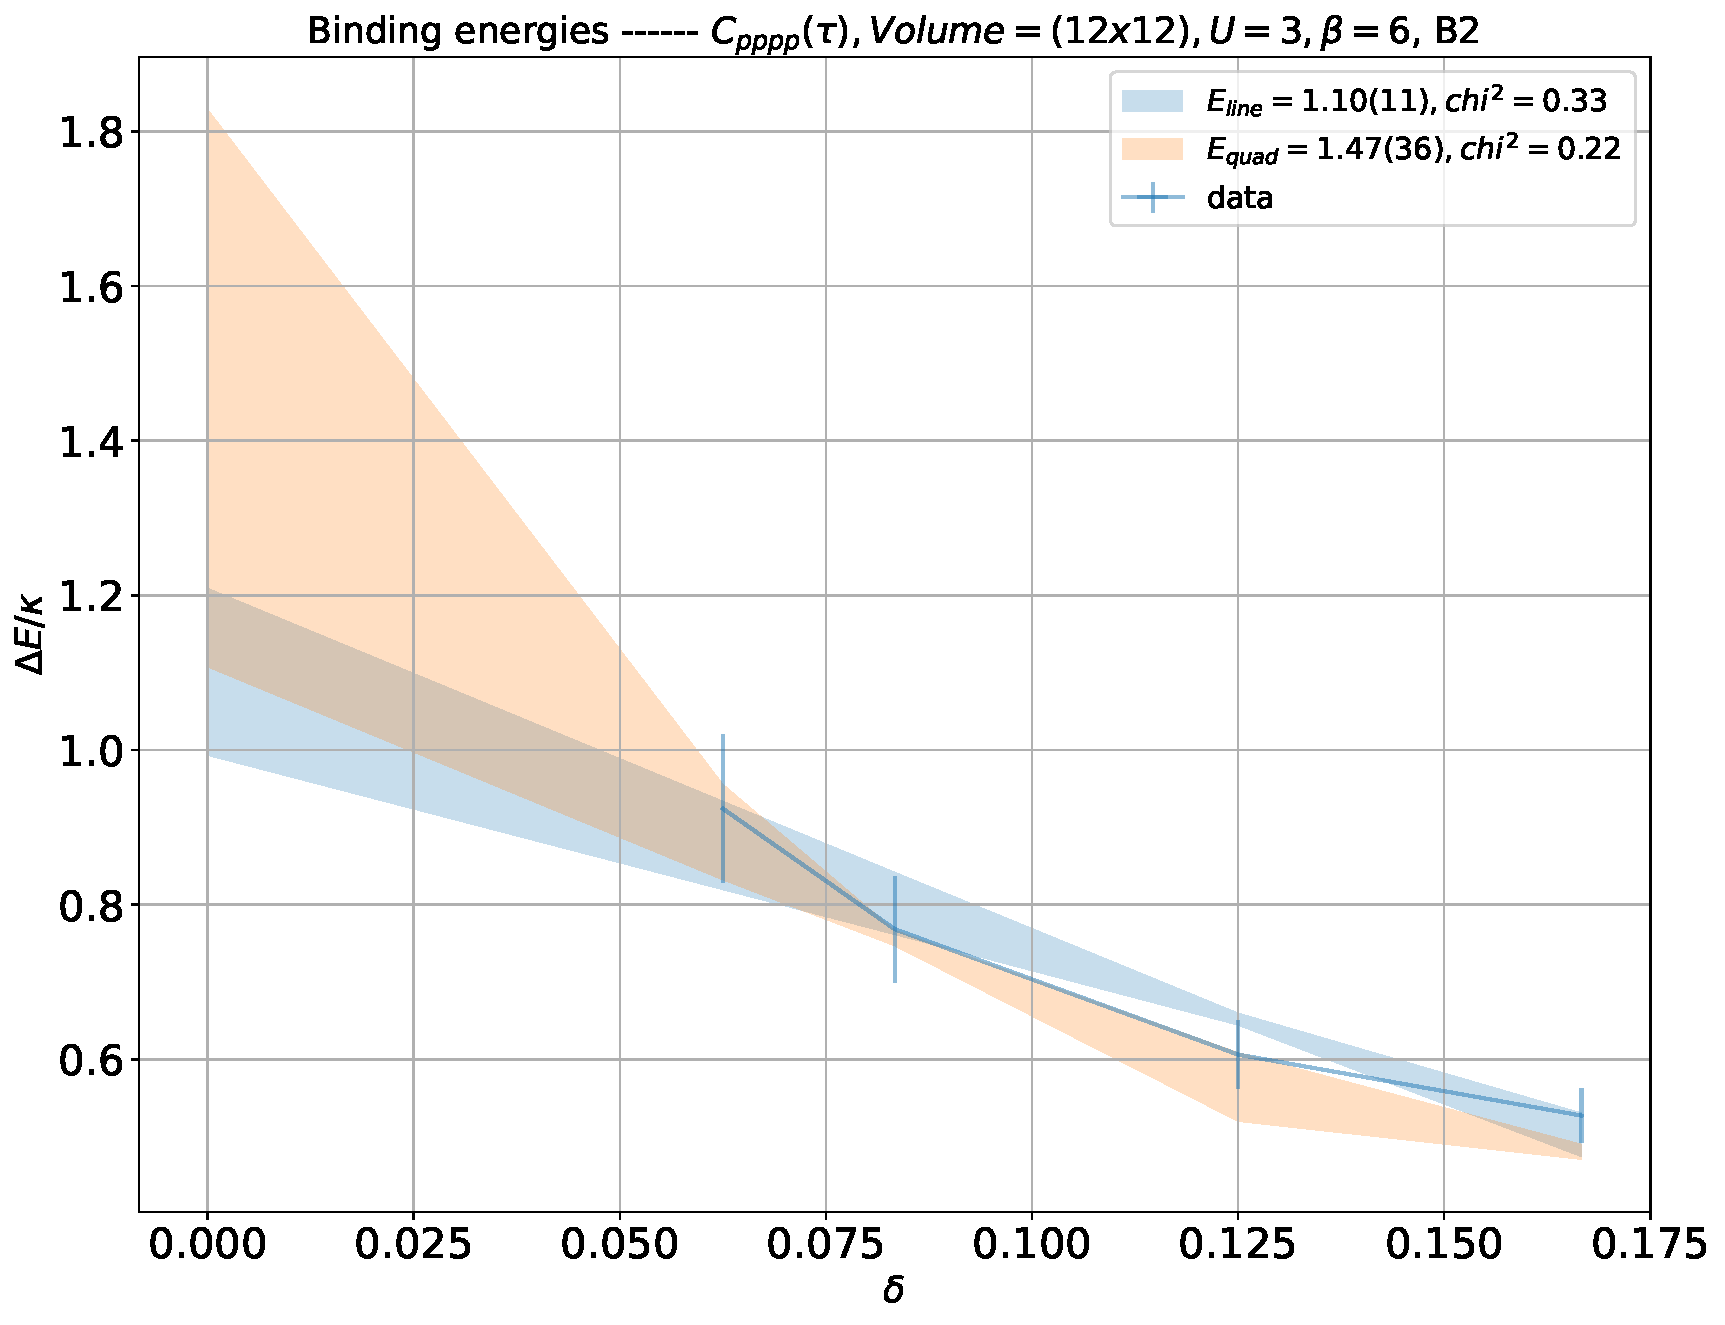
\includegraphics[width=\linewidth]{pppp-0-B2_12x12_U3_B6_cont.pdf}
  \end{subfigure}
  \caption{Binding energy extraction of the particle-particle pair at both irreducible representations, where we fit one- and two-body correlators for every $N_t$. This is followed by fitting a linear and a quadratic functions to the $\Delta E_{N_t}$ in order to extrapolate to the continuum limit ($N_t\to\infty$).}
  \label{fig:fig8}
\end{figure}

\begin{figure}
  \begin{subfigure}{.5\textwidth}
    \centering
    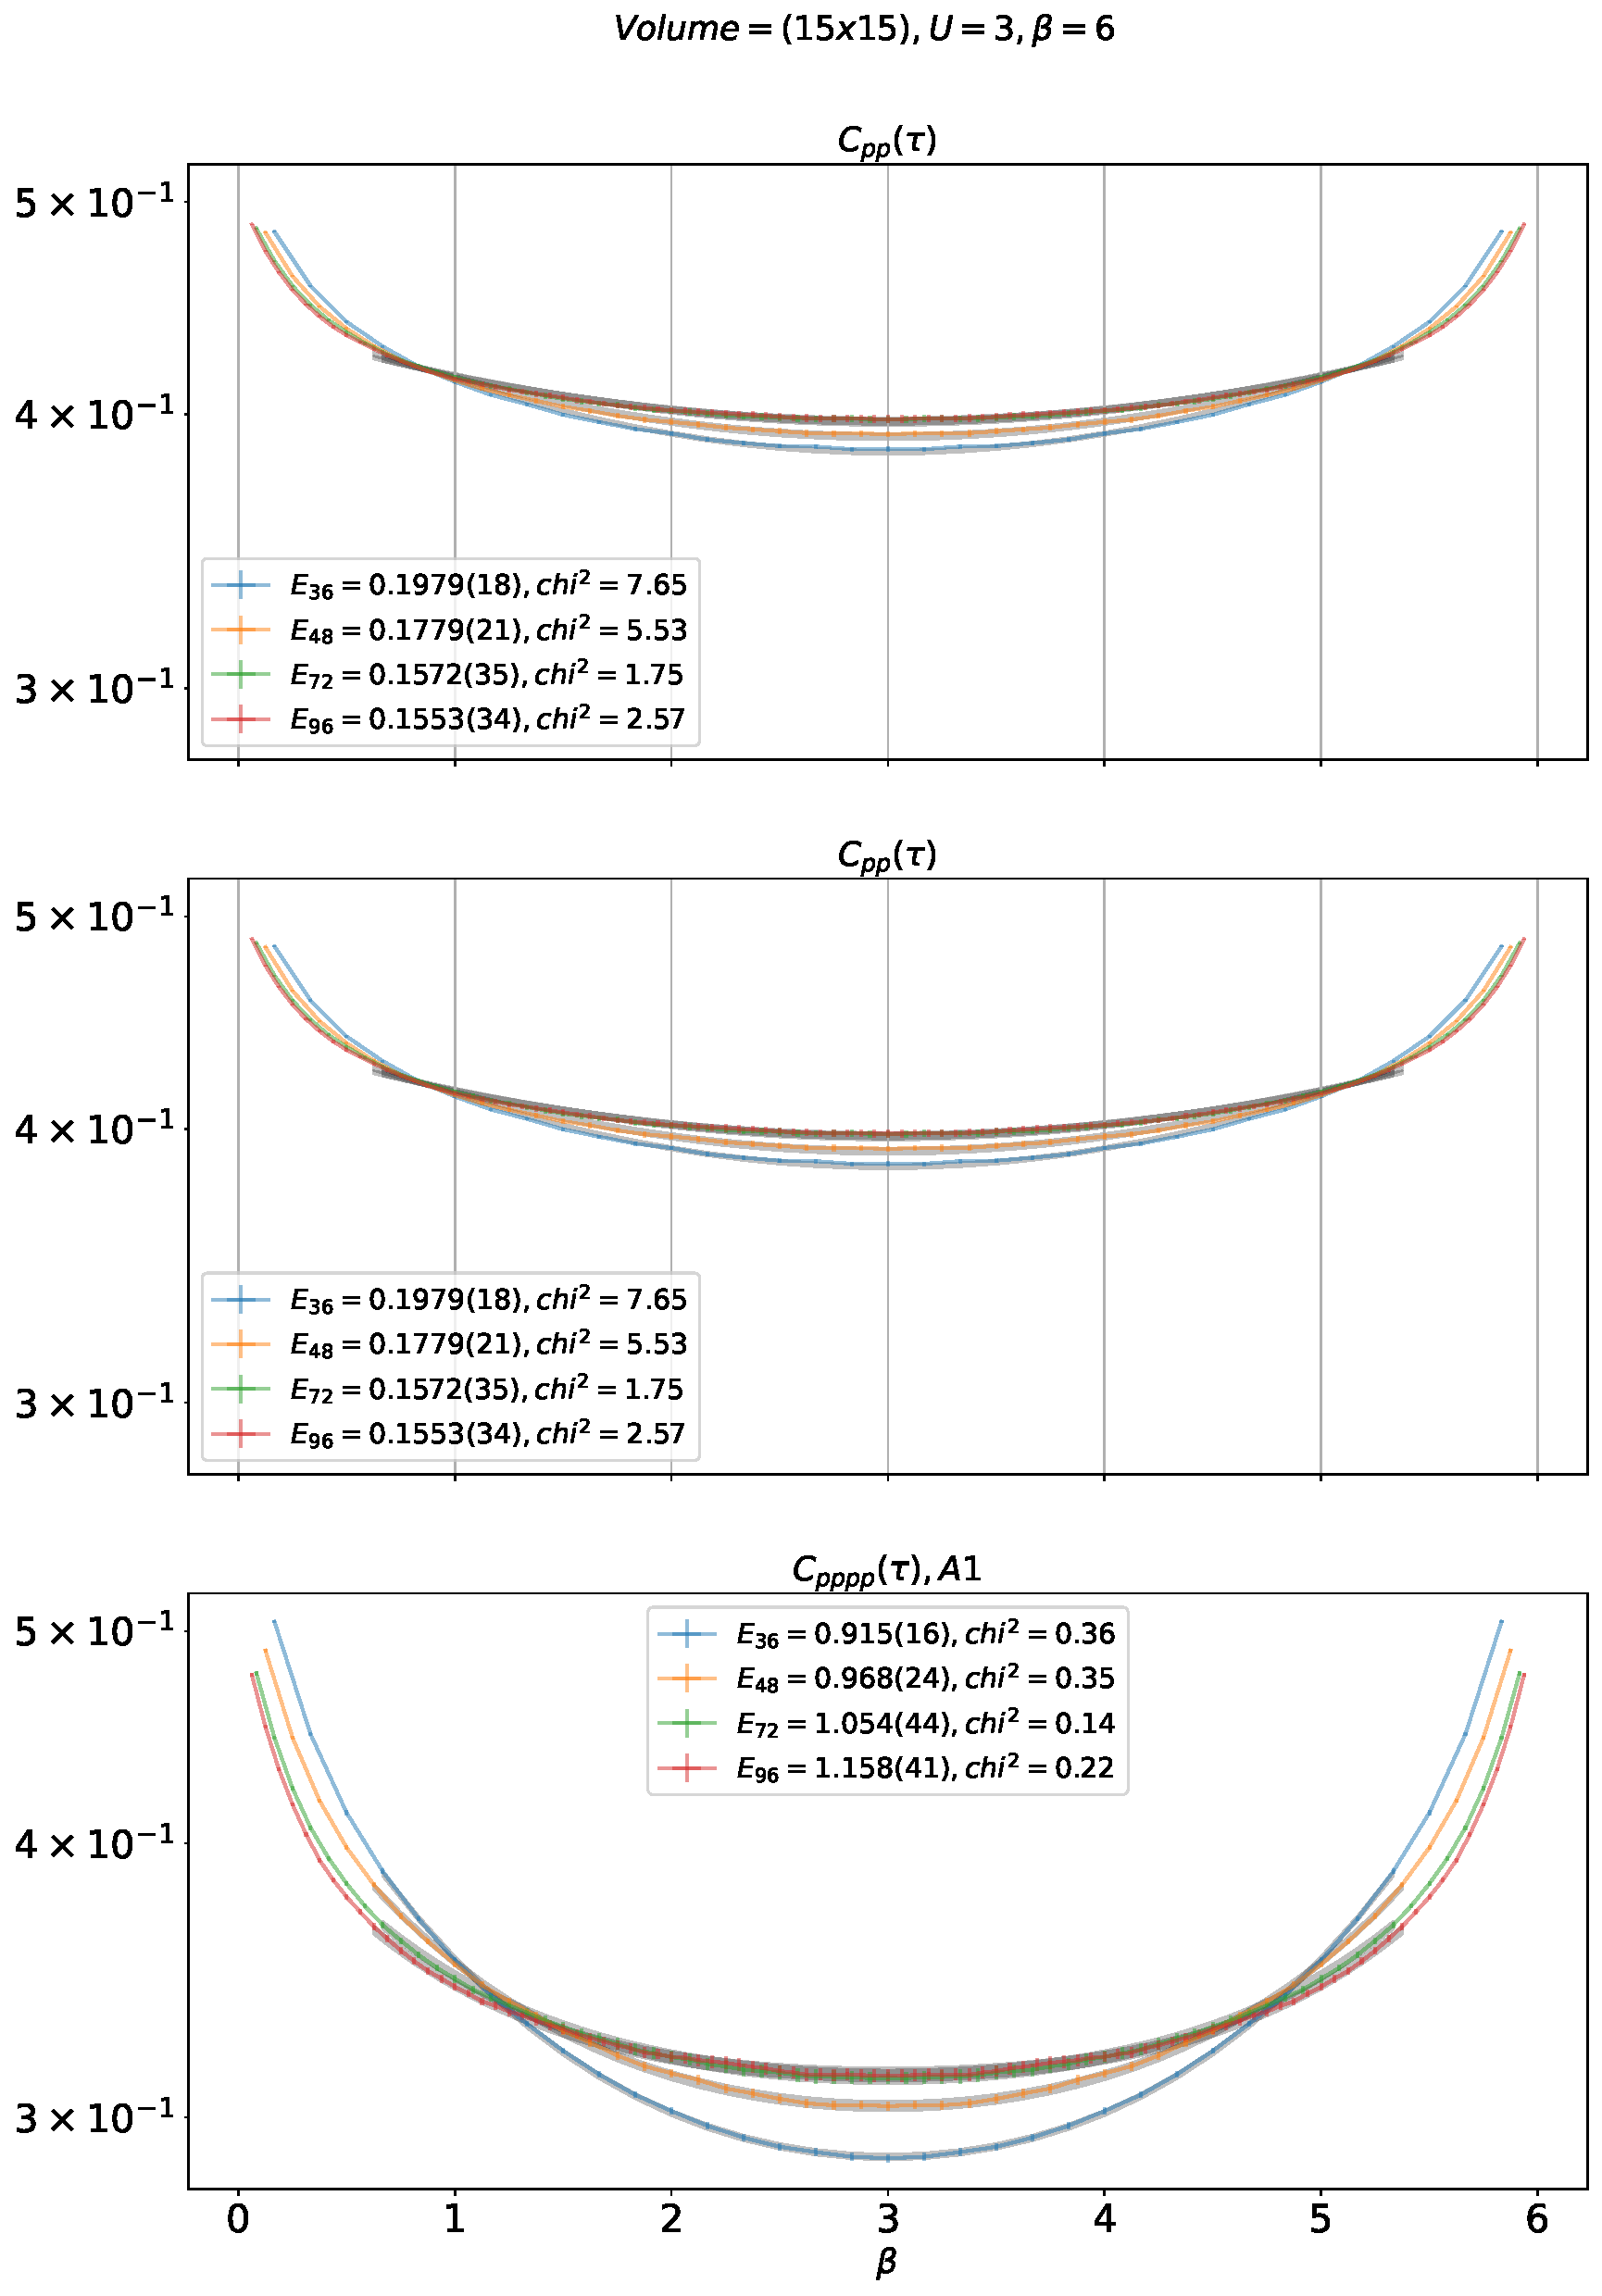
\includegraphics[width=\linewidth]{pppp-0-A1_15x15_U3_B6.pdf}
  \end{subfigure}%
  \begin{subfigure}{.5\textwidth}
    \centering
    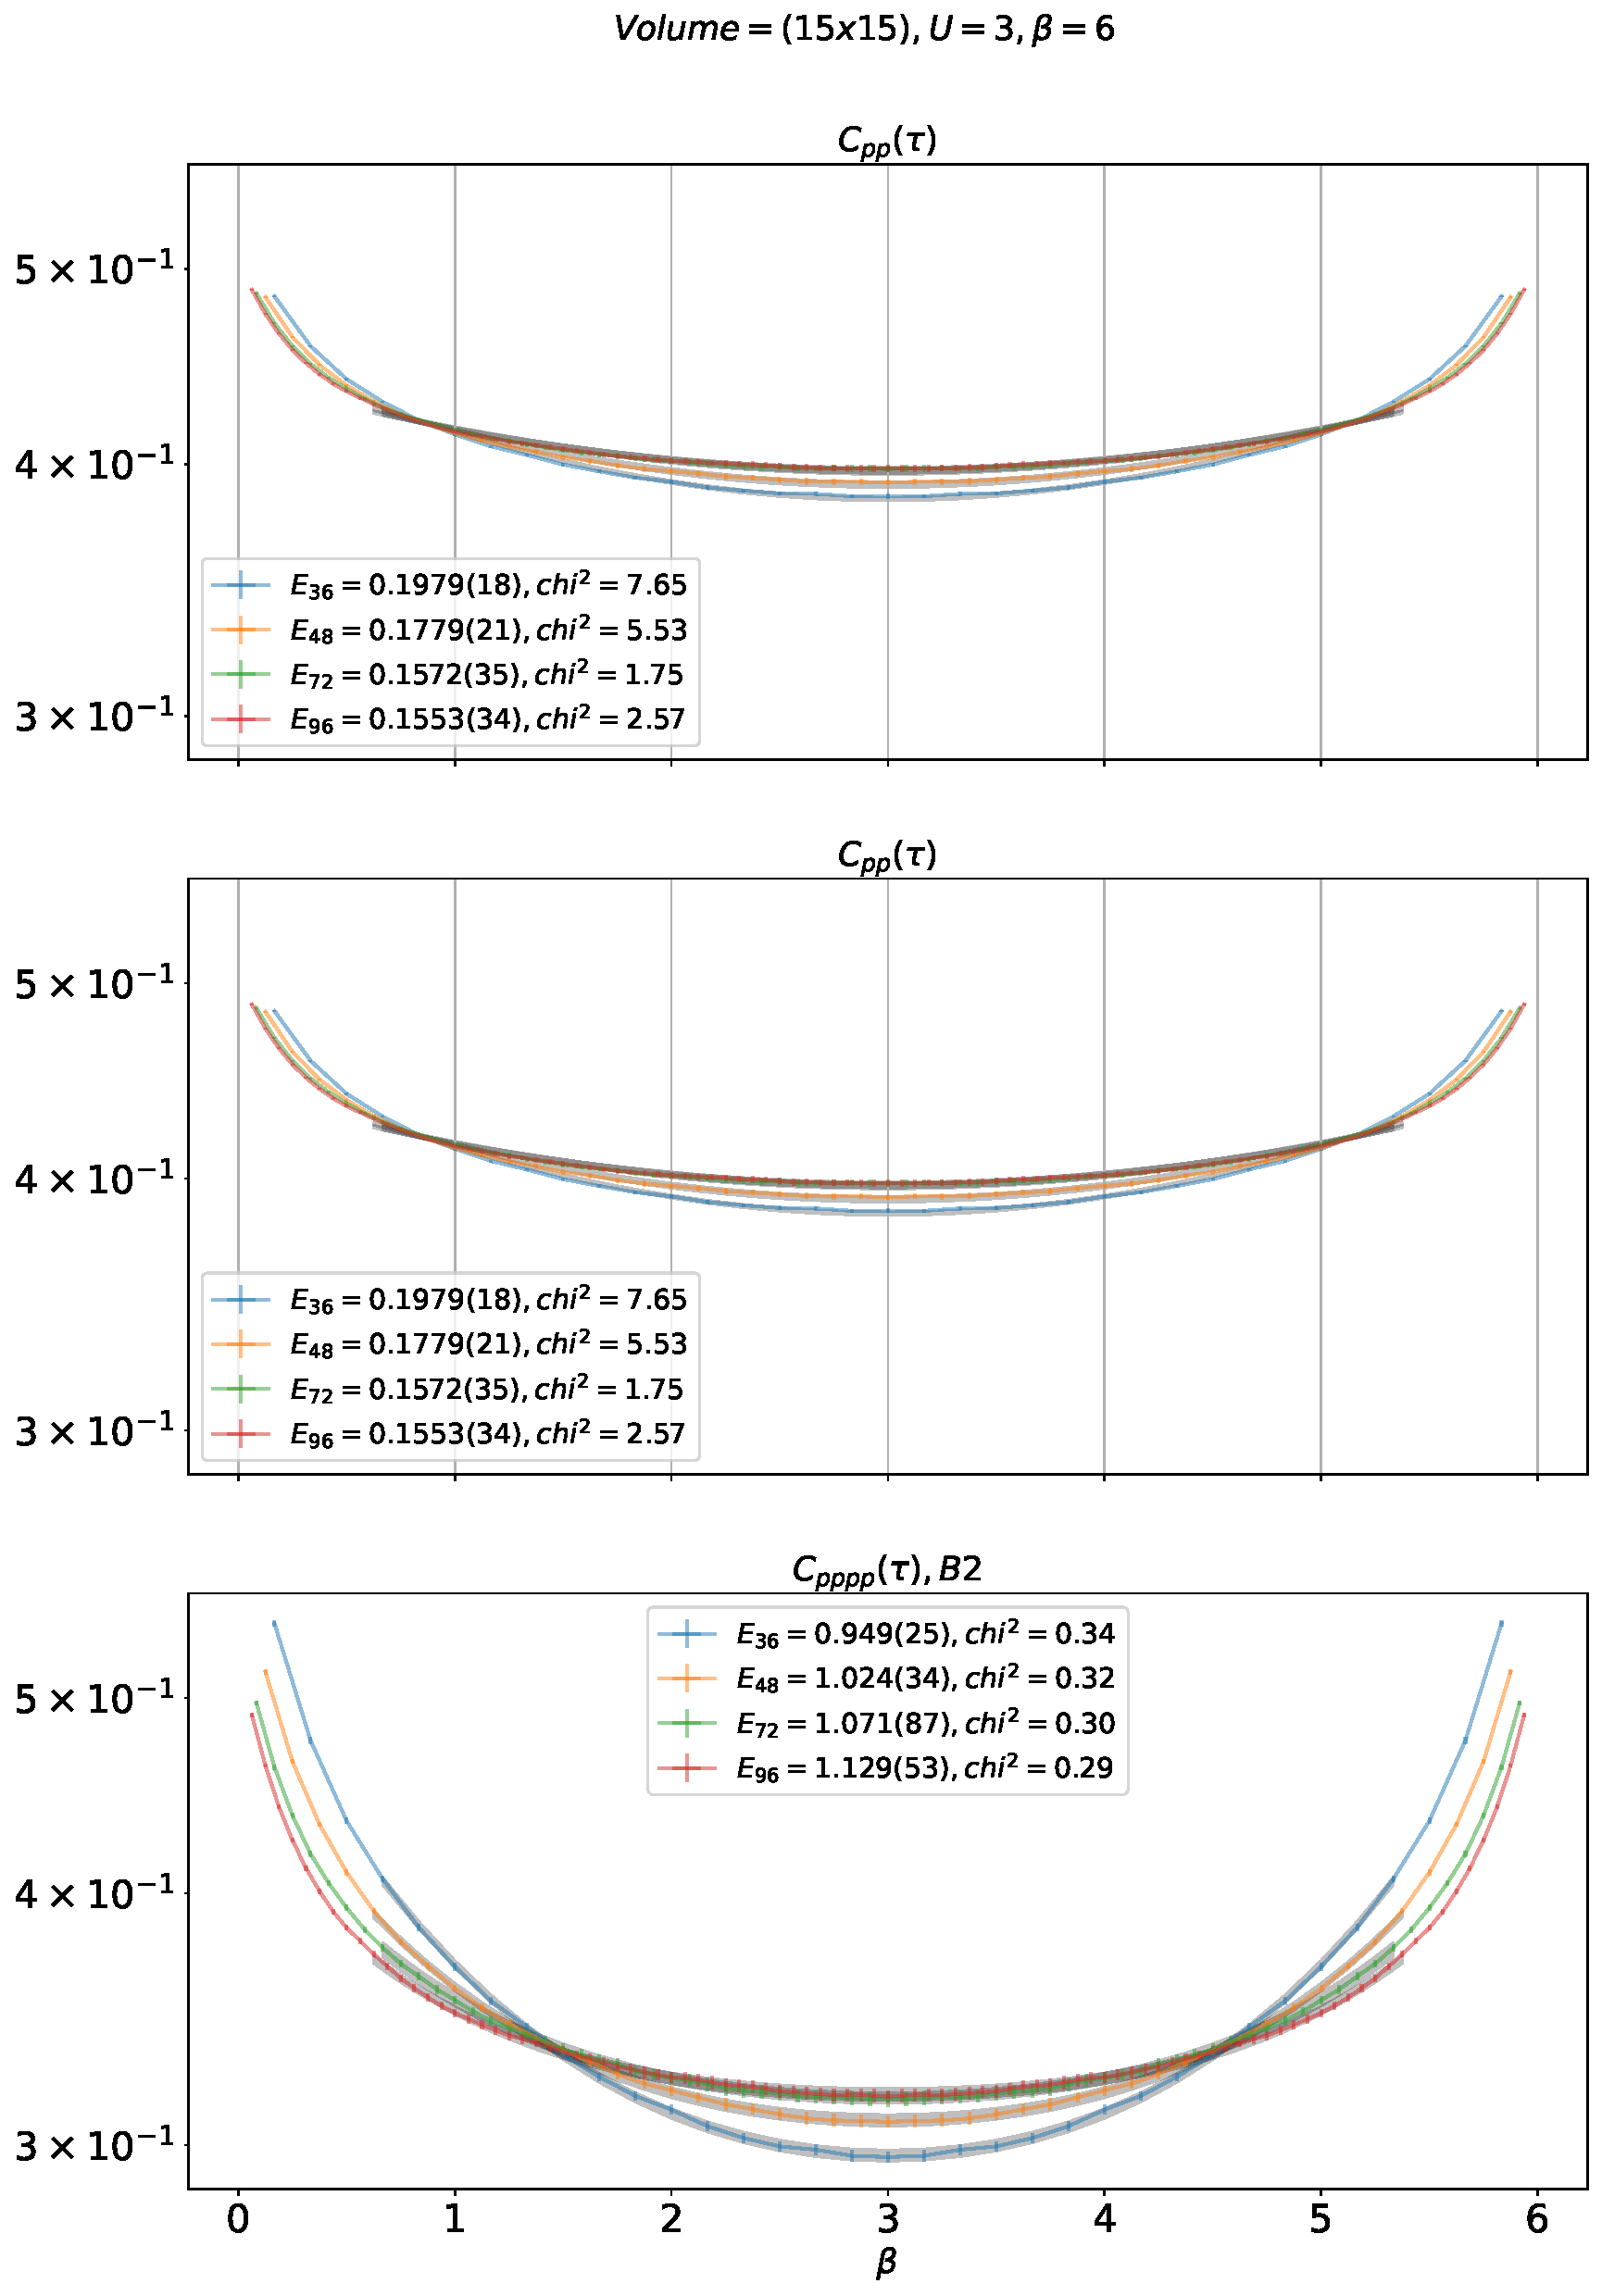
\includegraphics[width=\linewidth]{pppp-0-B2_15x15_U3_B6.pdf}
  \end{subfigure}
  \begin{subfigure}{.5\textwidth}
      \centering
      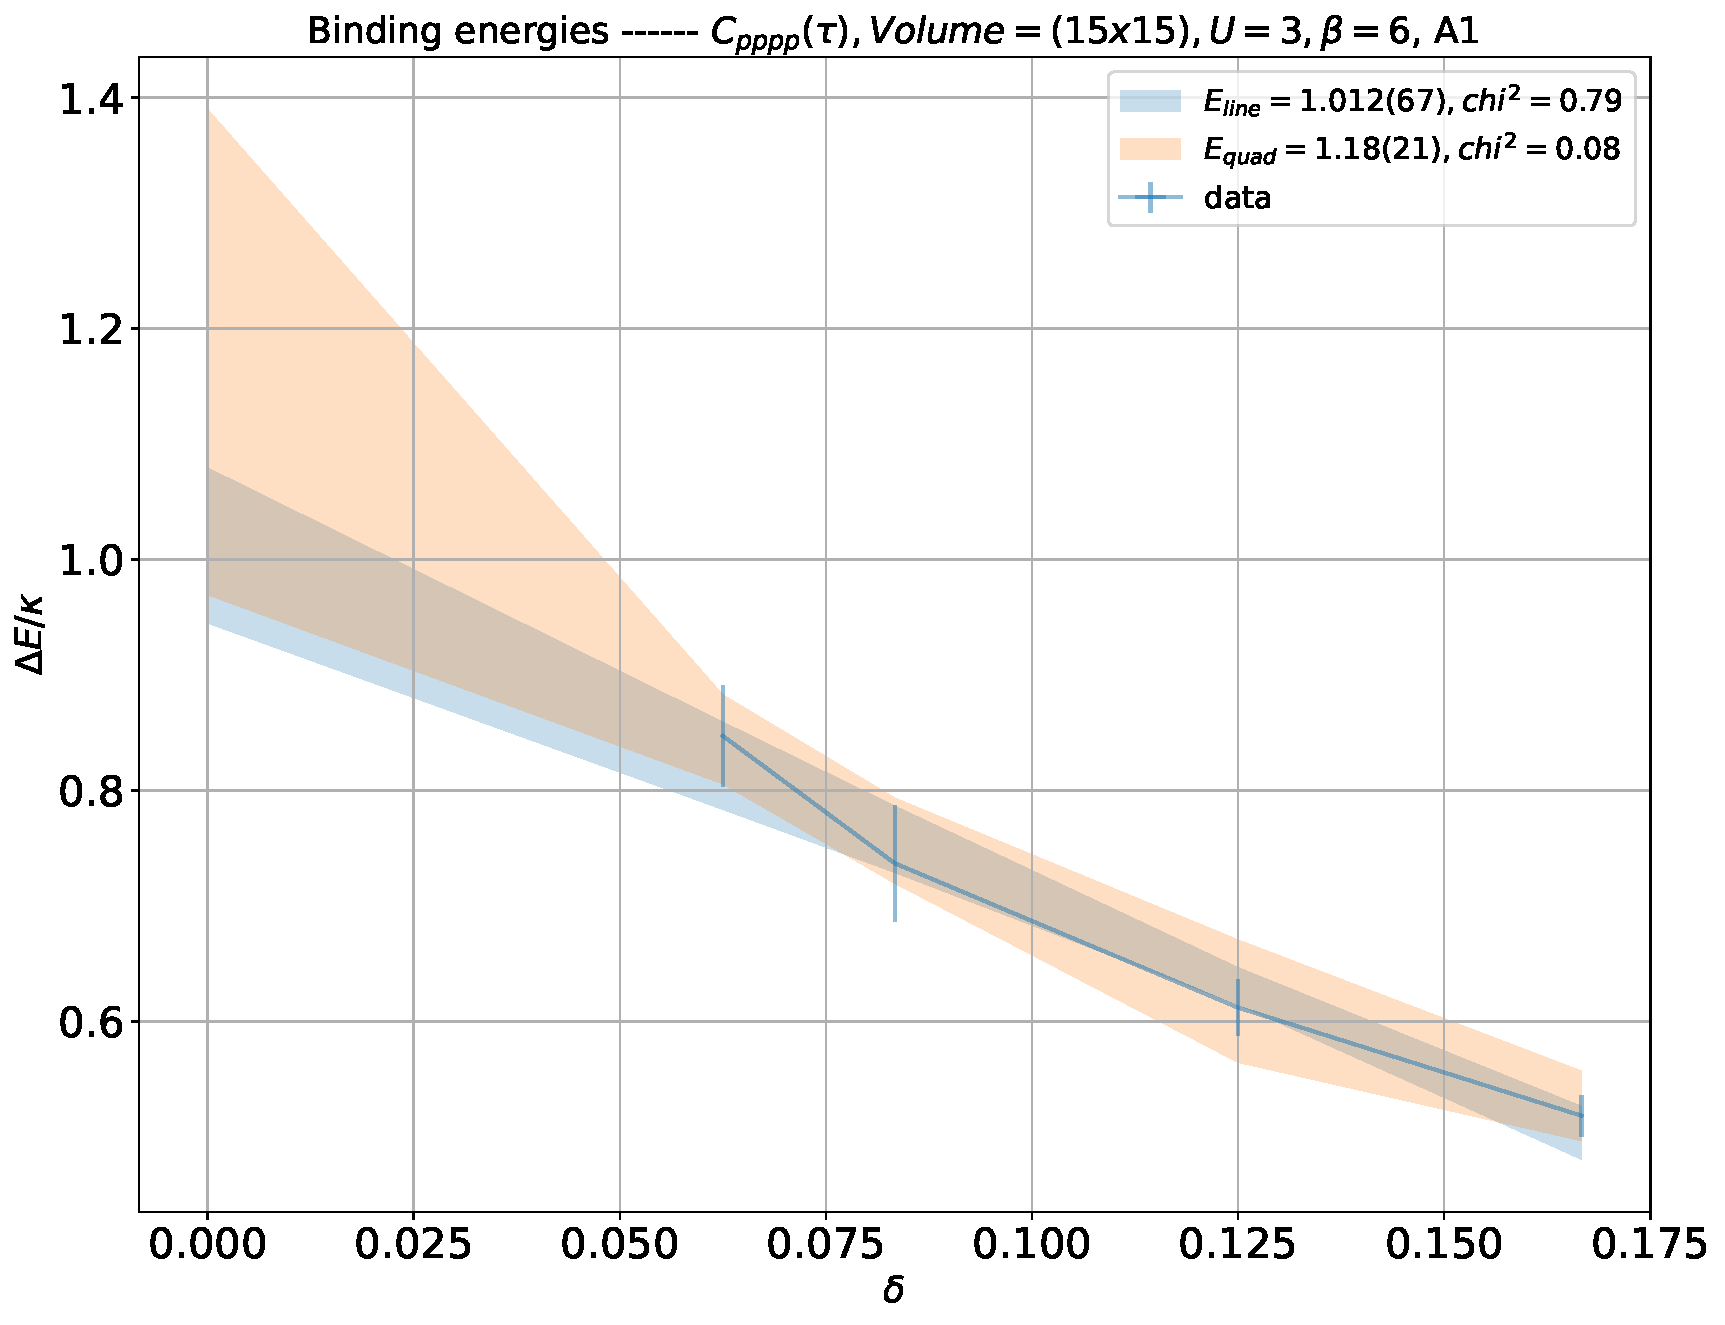
\includegraphics[width=\linewidth]{pppp-0-A1_15x15_U3_B6_cont.pdf}
  \end{subfigure}
  \begin{subfigure}{.5\textwidth}
      \centering
      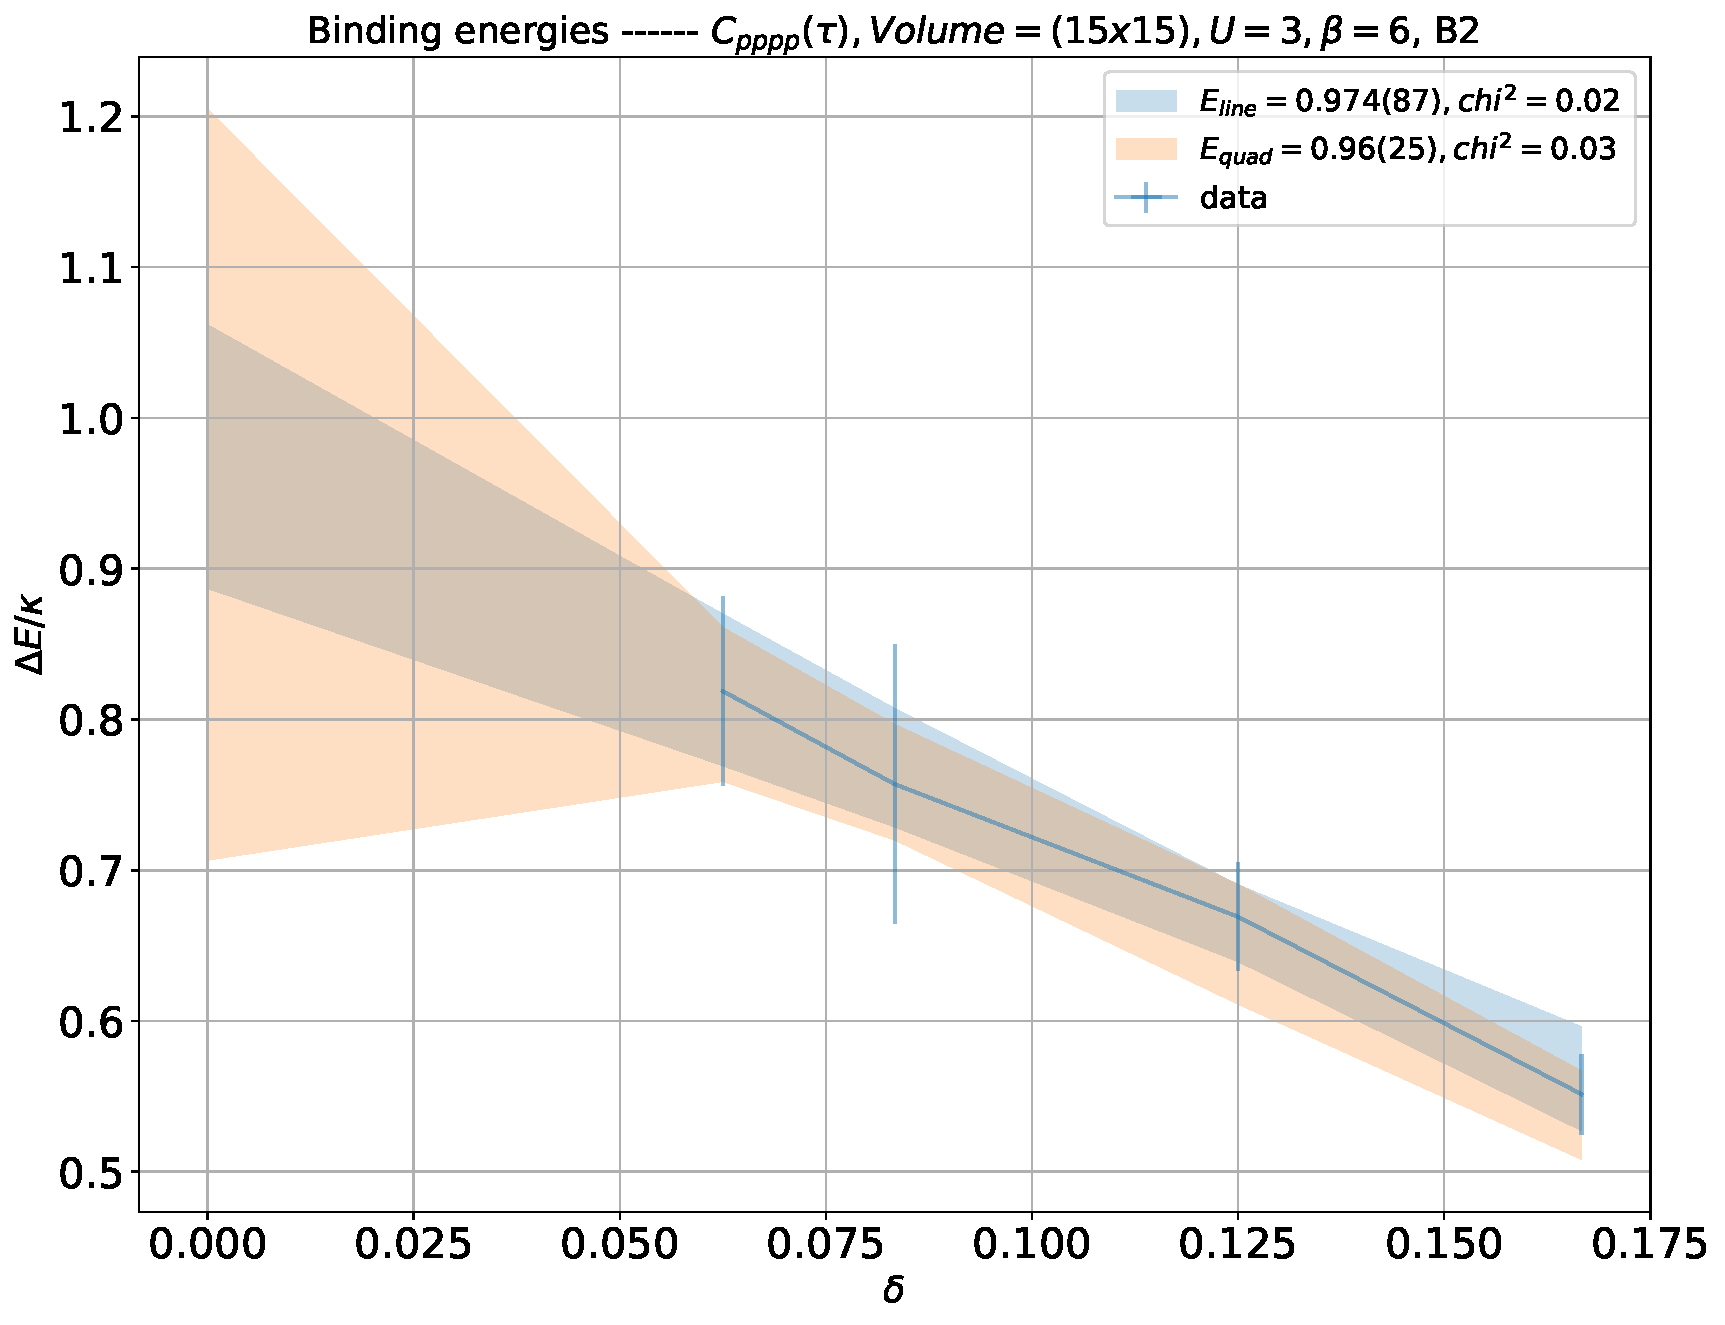
\includegraphics[width=\linewidth]{pppp-0-B2_15x15_U3_B6_cont.pdf}
  \end{subfigure}
  \caption{Binding energy extraction of the particle-particle pair at both irreducible representations, where we fit one- and two-body correlators for every $N_t$. This is followed by fitting a linear and a quadratic functions to the $\Delta E_{N_t}$ in order to extrapolate to the continuum limit ($N_t\to\infty$).}
  \label{fig:fig9}
\end{figure}

\begin{figure}
  \begin{subfigure}{.5\textwidth}
    \centering
    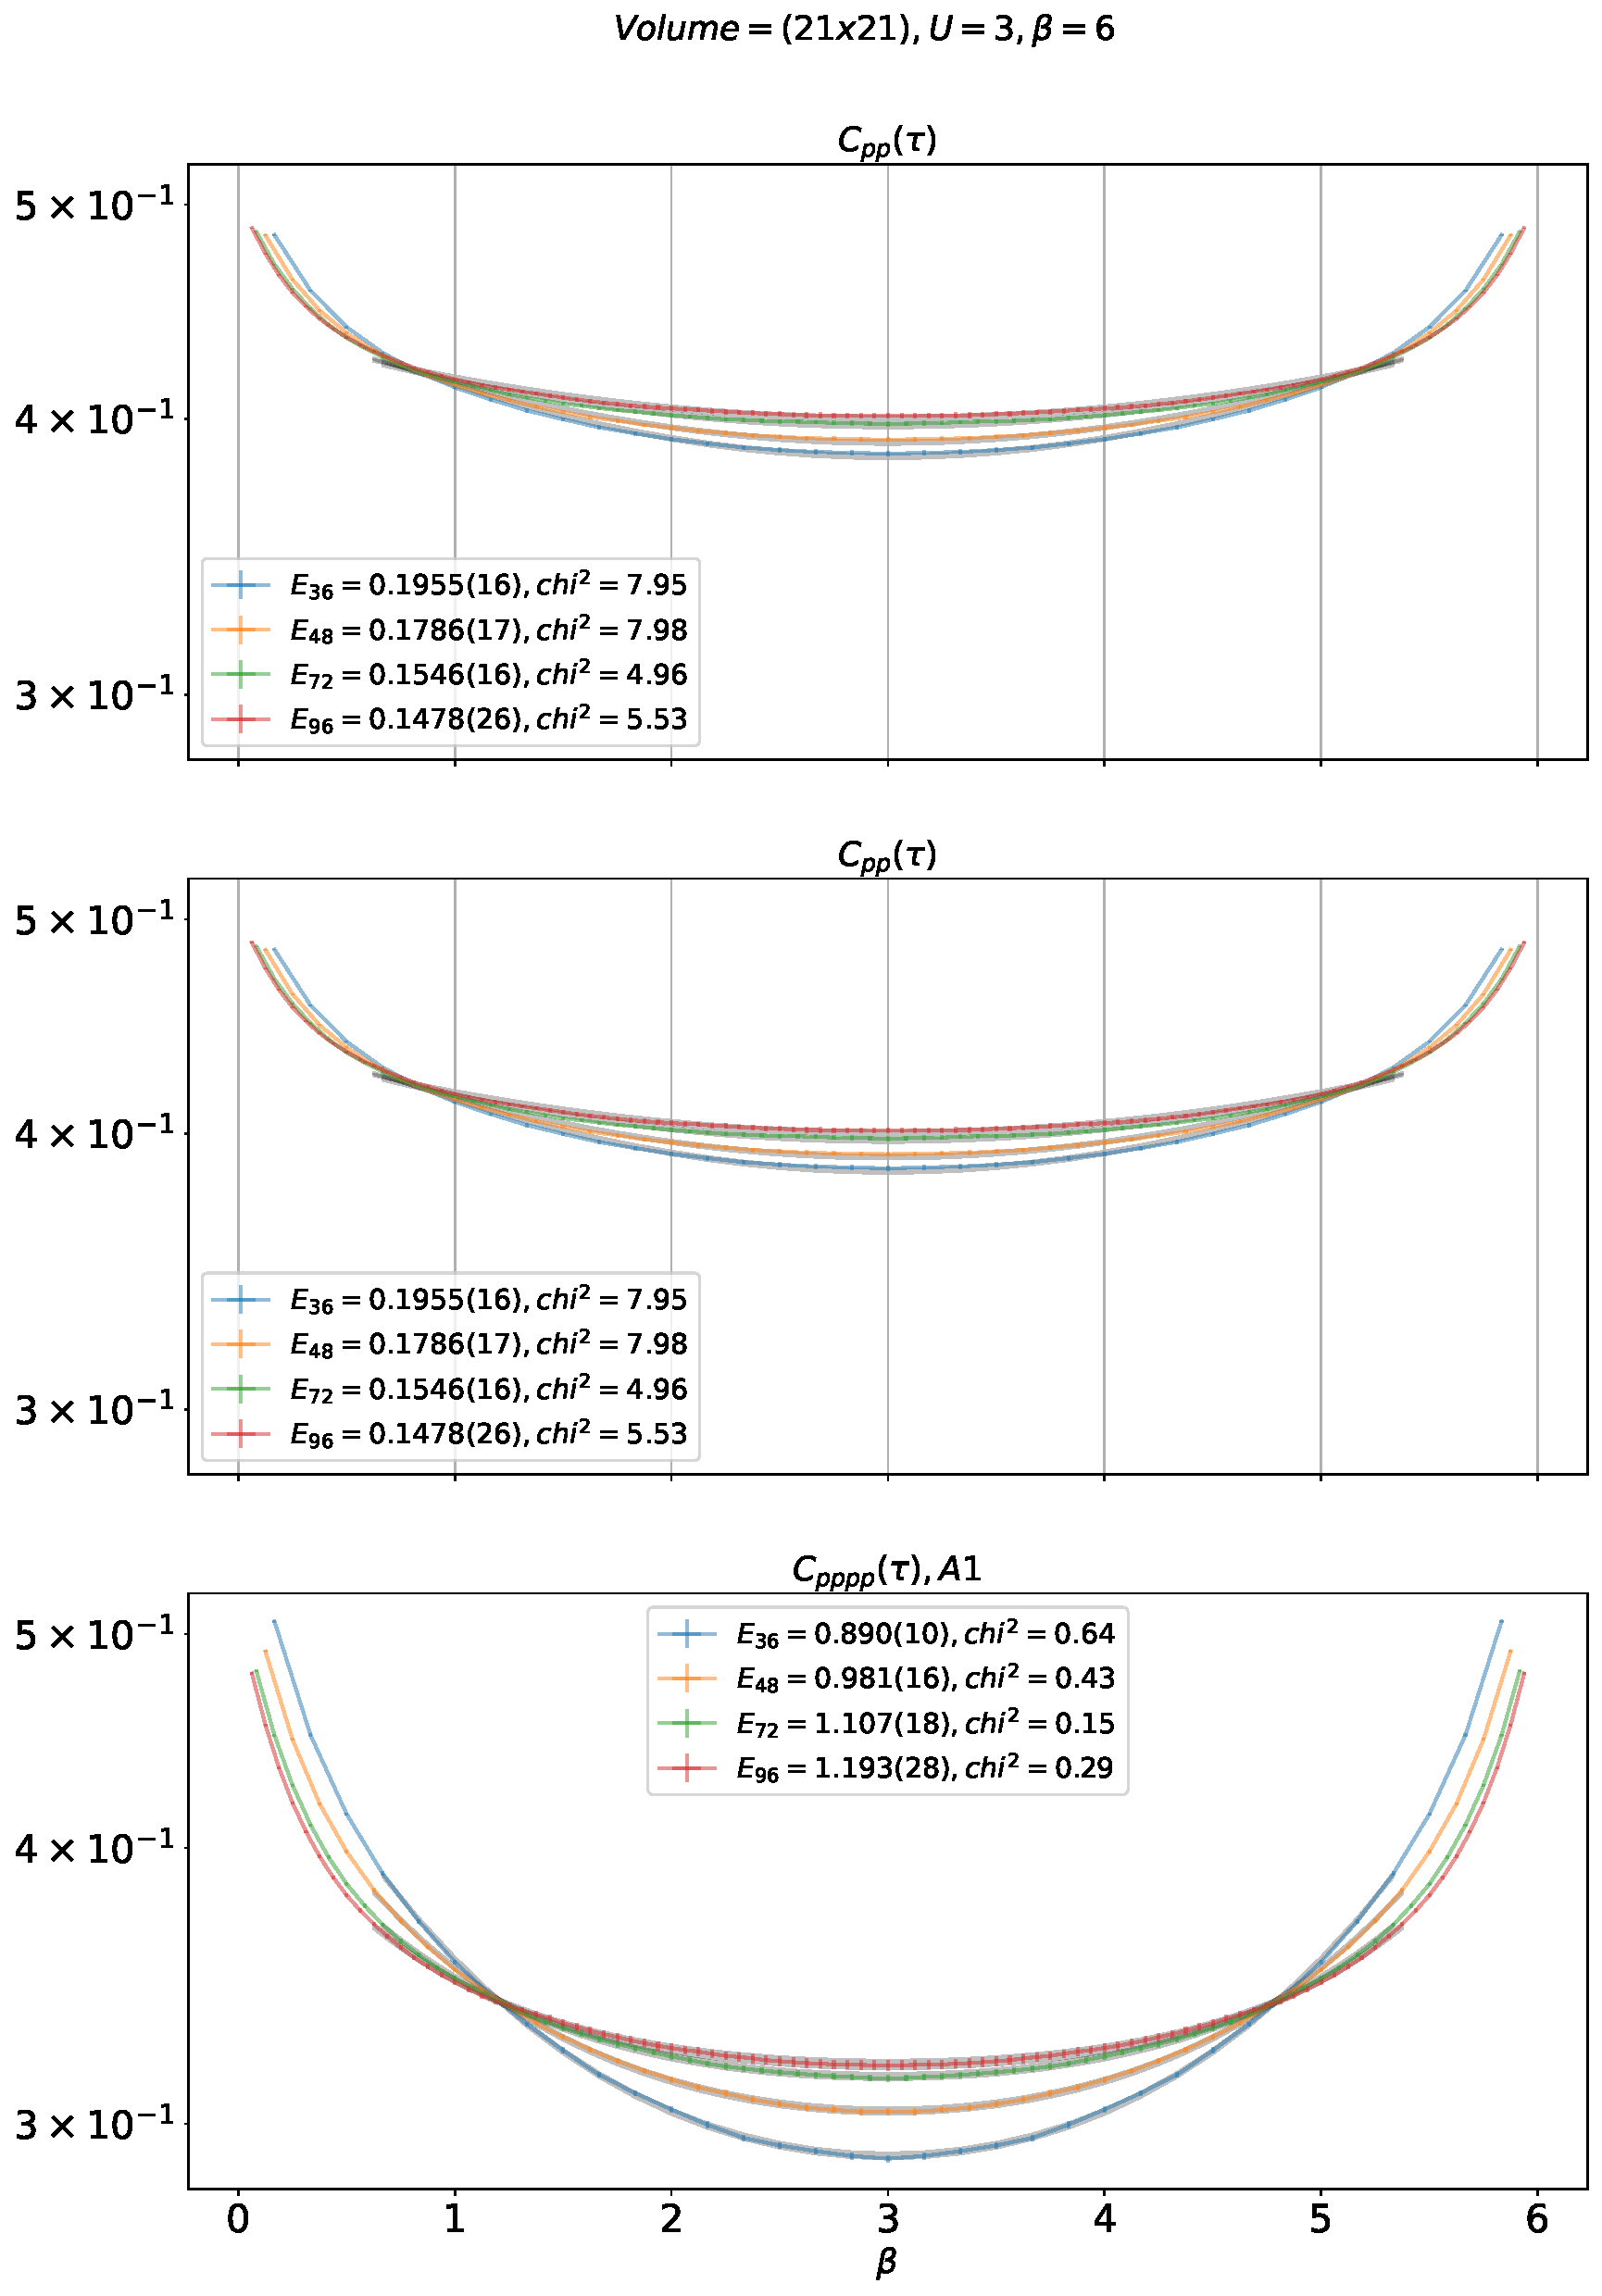
\includegraphics[width=\linewidth]{pppp-0-A1_21x21_U3_B6.pdf}
  \end{subfigure}%
  \begin{subfigure}{.5\textwidth}
    \centering
    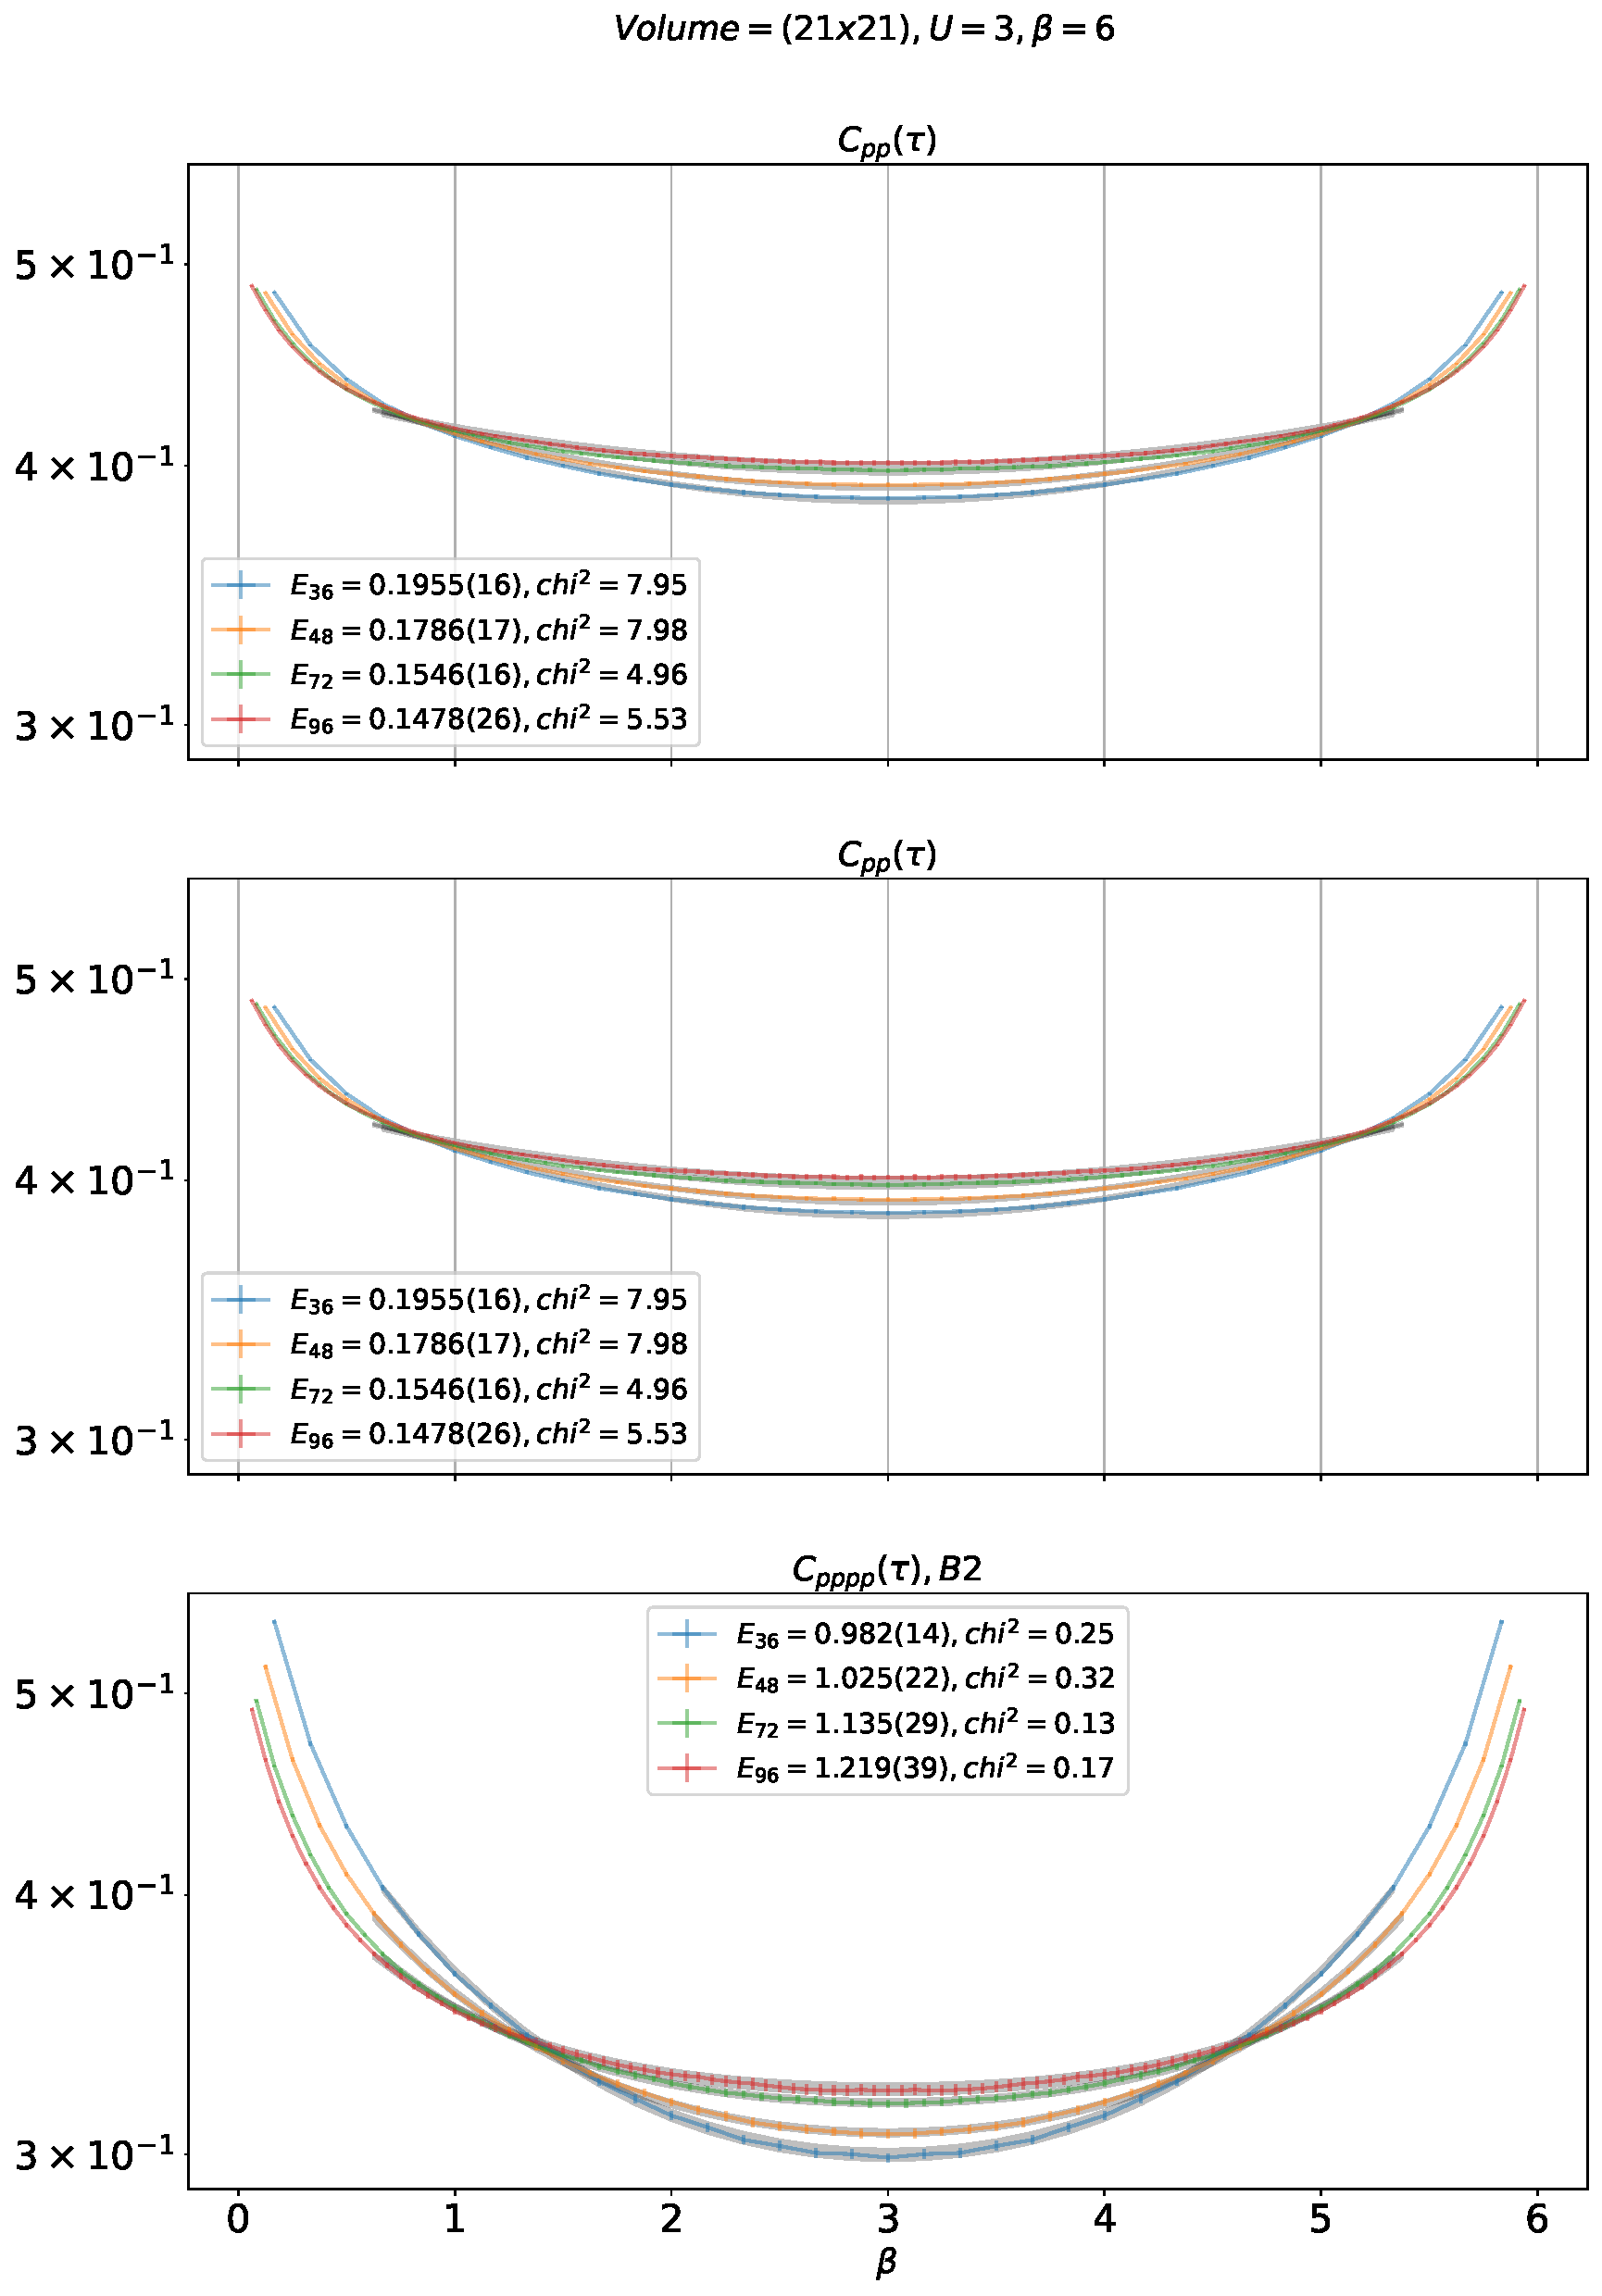
\includegraphics[width=\linewidth]{pppp-0-B2_21x21_U3_B6.pdf}
  \end{subfigure}
  \begin{subfigure}{.5\textwidth}
      \centering
      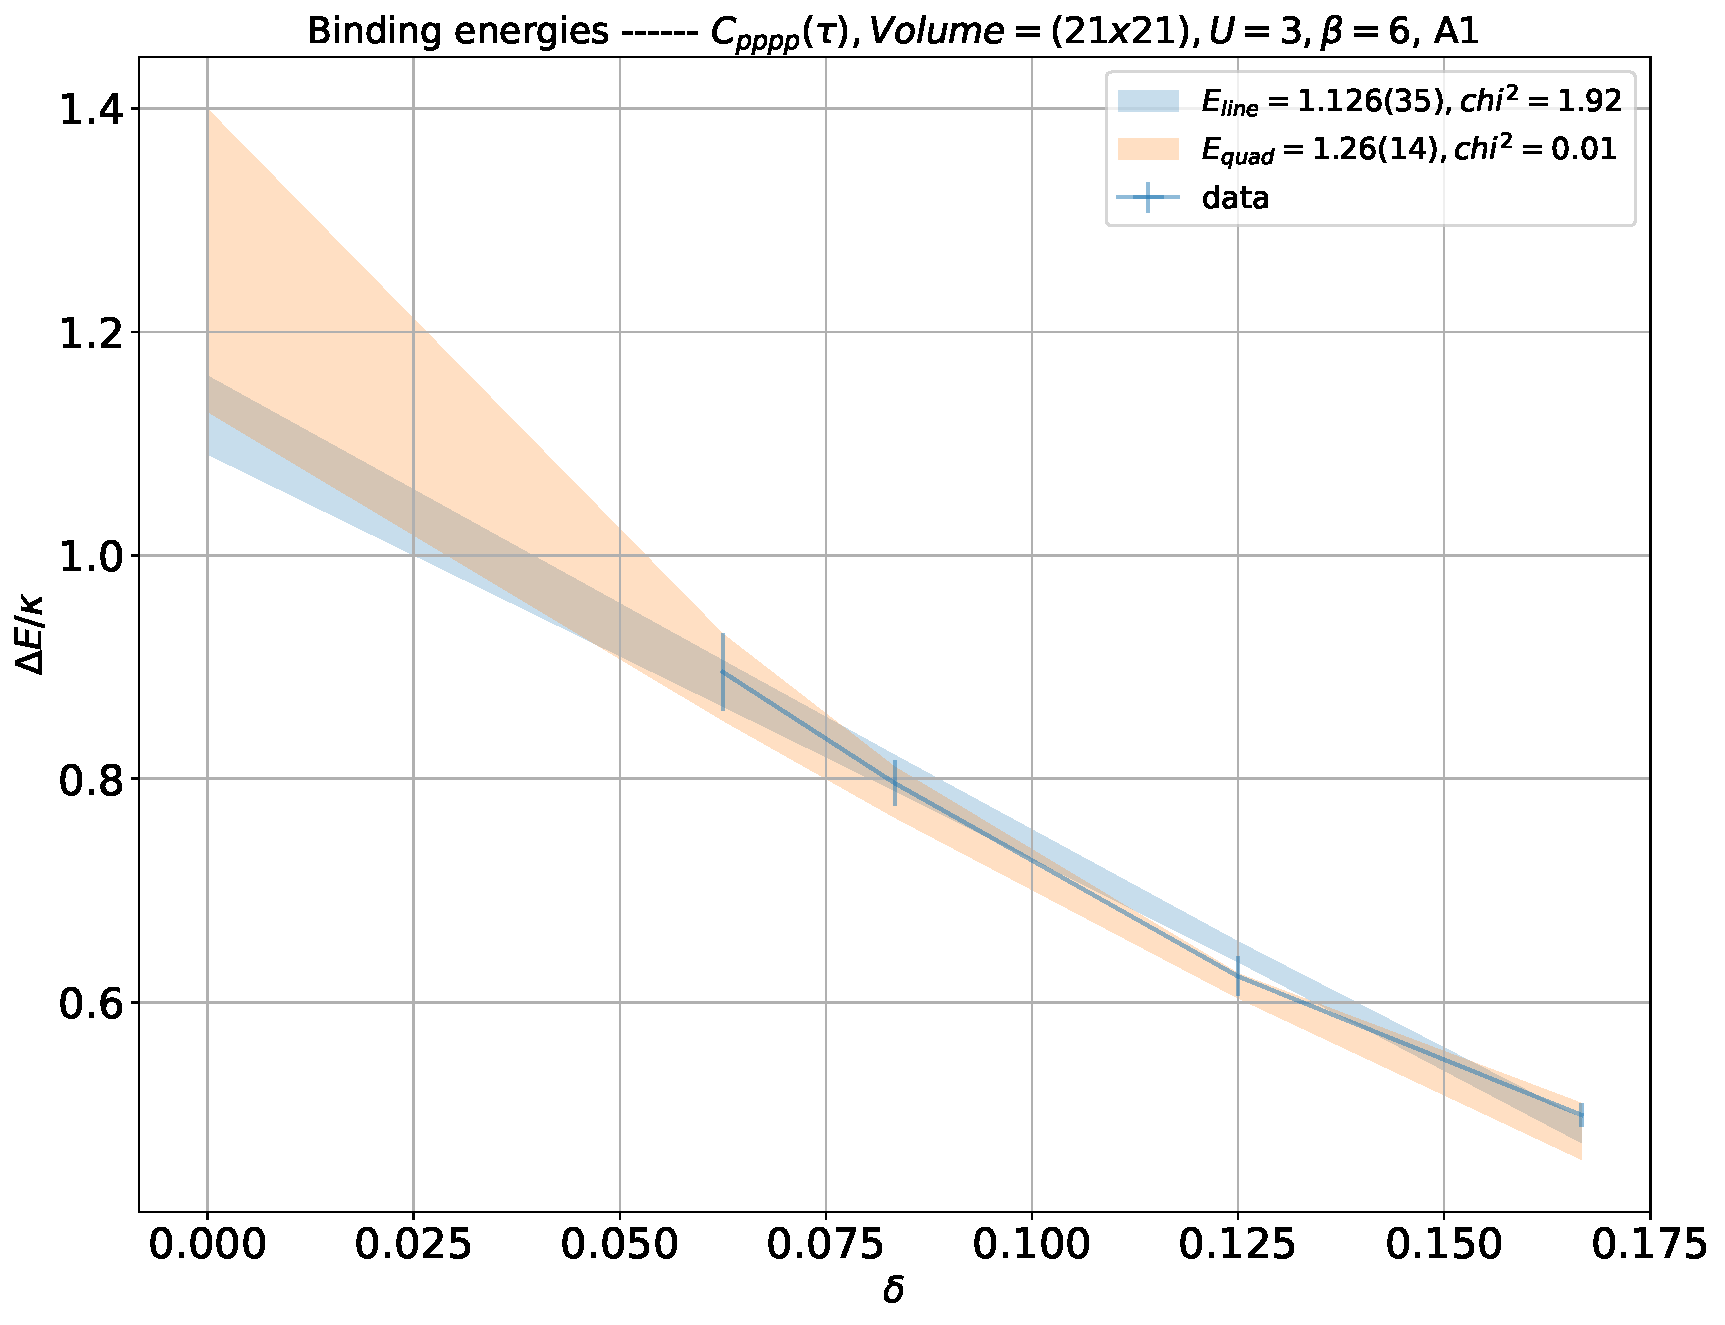
\includegraphics[width=\linewidth]{pppp-0-A1_21x21_U3_B6_cont.pdf}
  \end{subfigure}
  \begin{subfigure}{.5\textwidth}
      \centering
      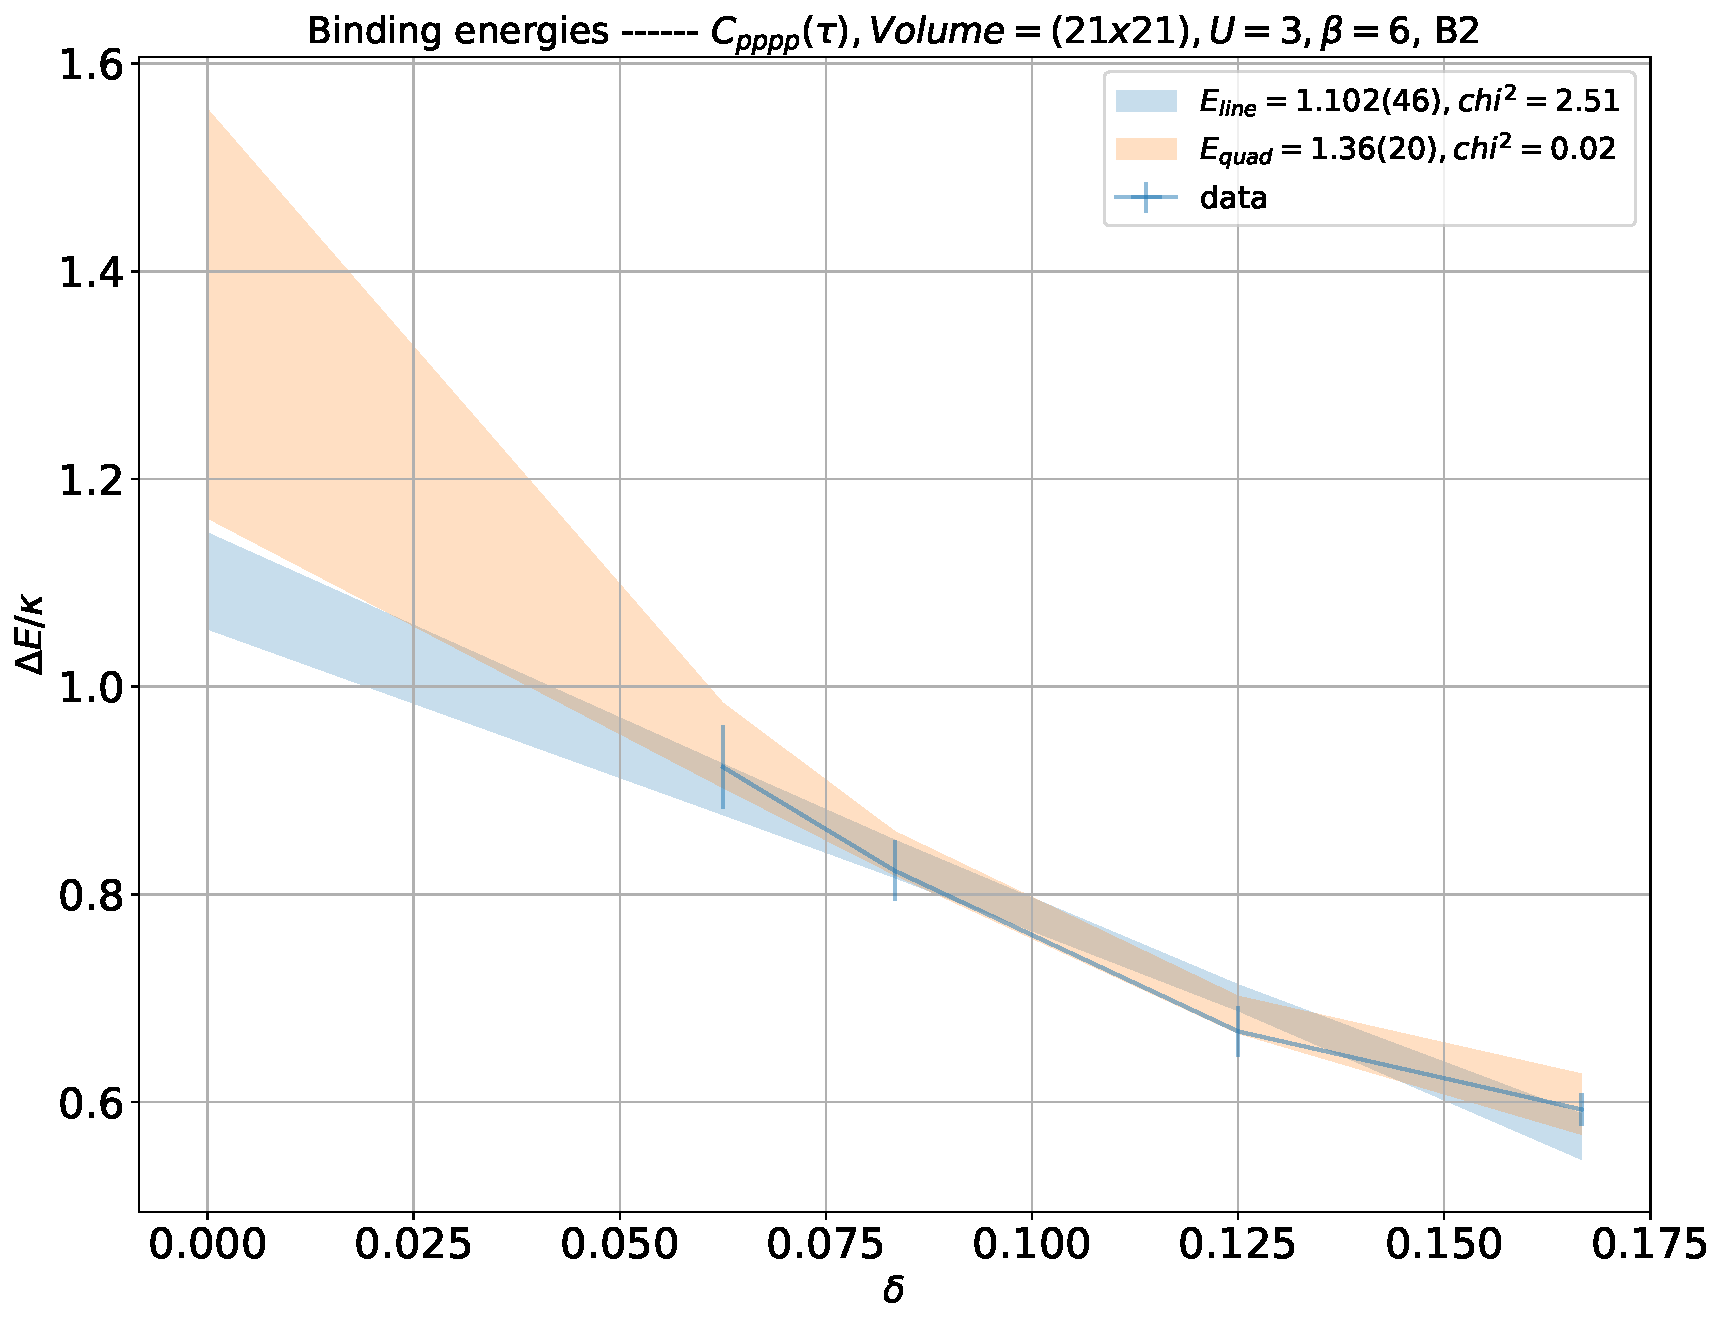
\includegraphics[width=\linewidth]{pppp-0-B2_21x21_U3_B6_cont.pdf}
  \end{subfigure}
  \caption{Binding energy extraction of the particle-particle pair at both irreducible representations, where we fit one- and two-body correlators for every $N_t$. This is followed by fitting a linear and a quadratic functions to the $\Delta E_{N_t}$ in order to extrapolate to the continuum limit ($N_t\to\infty$).}
  \label{fig:fig10}
\end{figure}
 
\begin{figure}
  \begin{subfigure}{.5\textwidth}
    \centering
    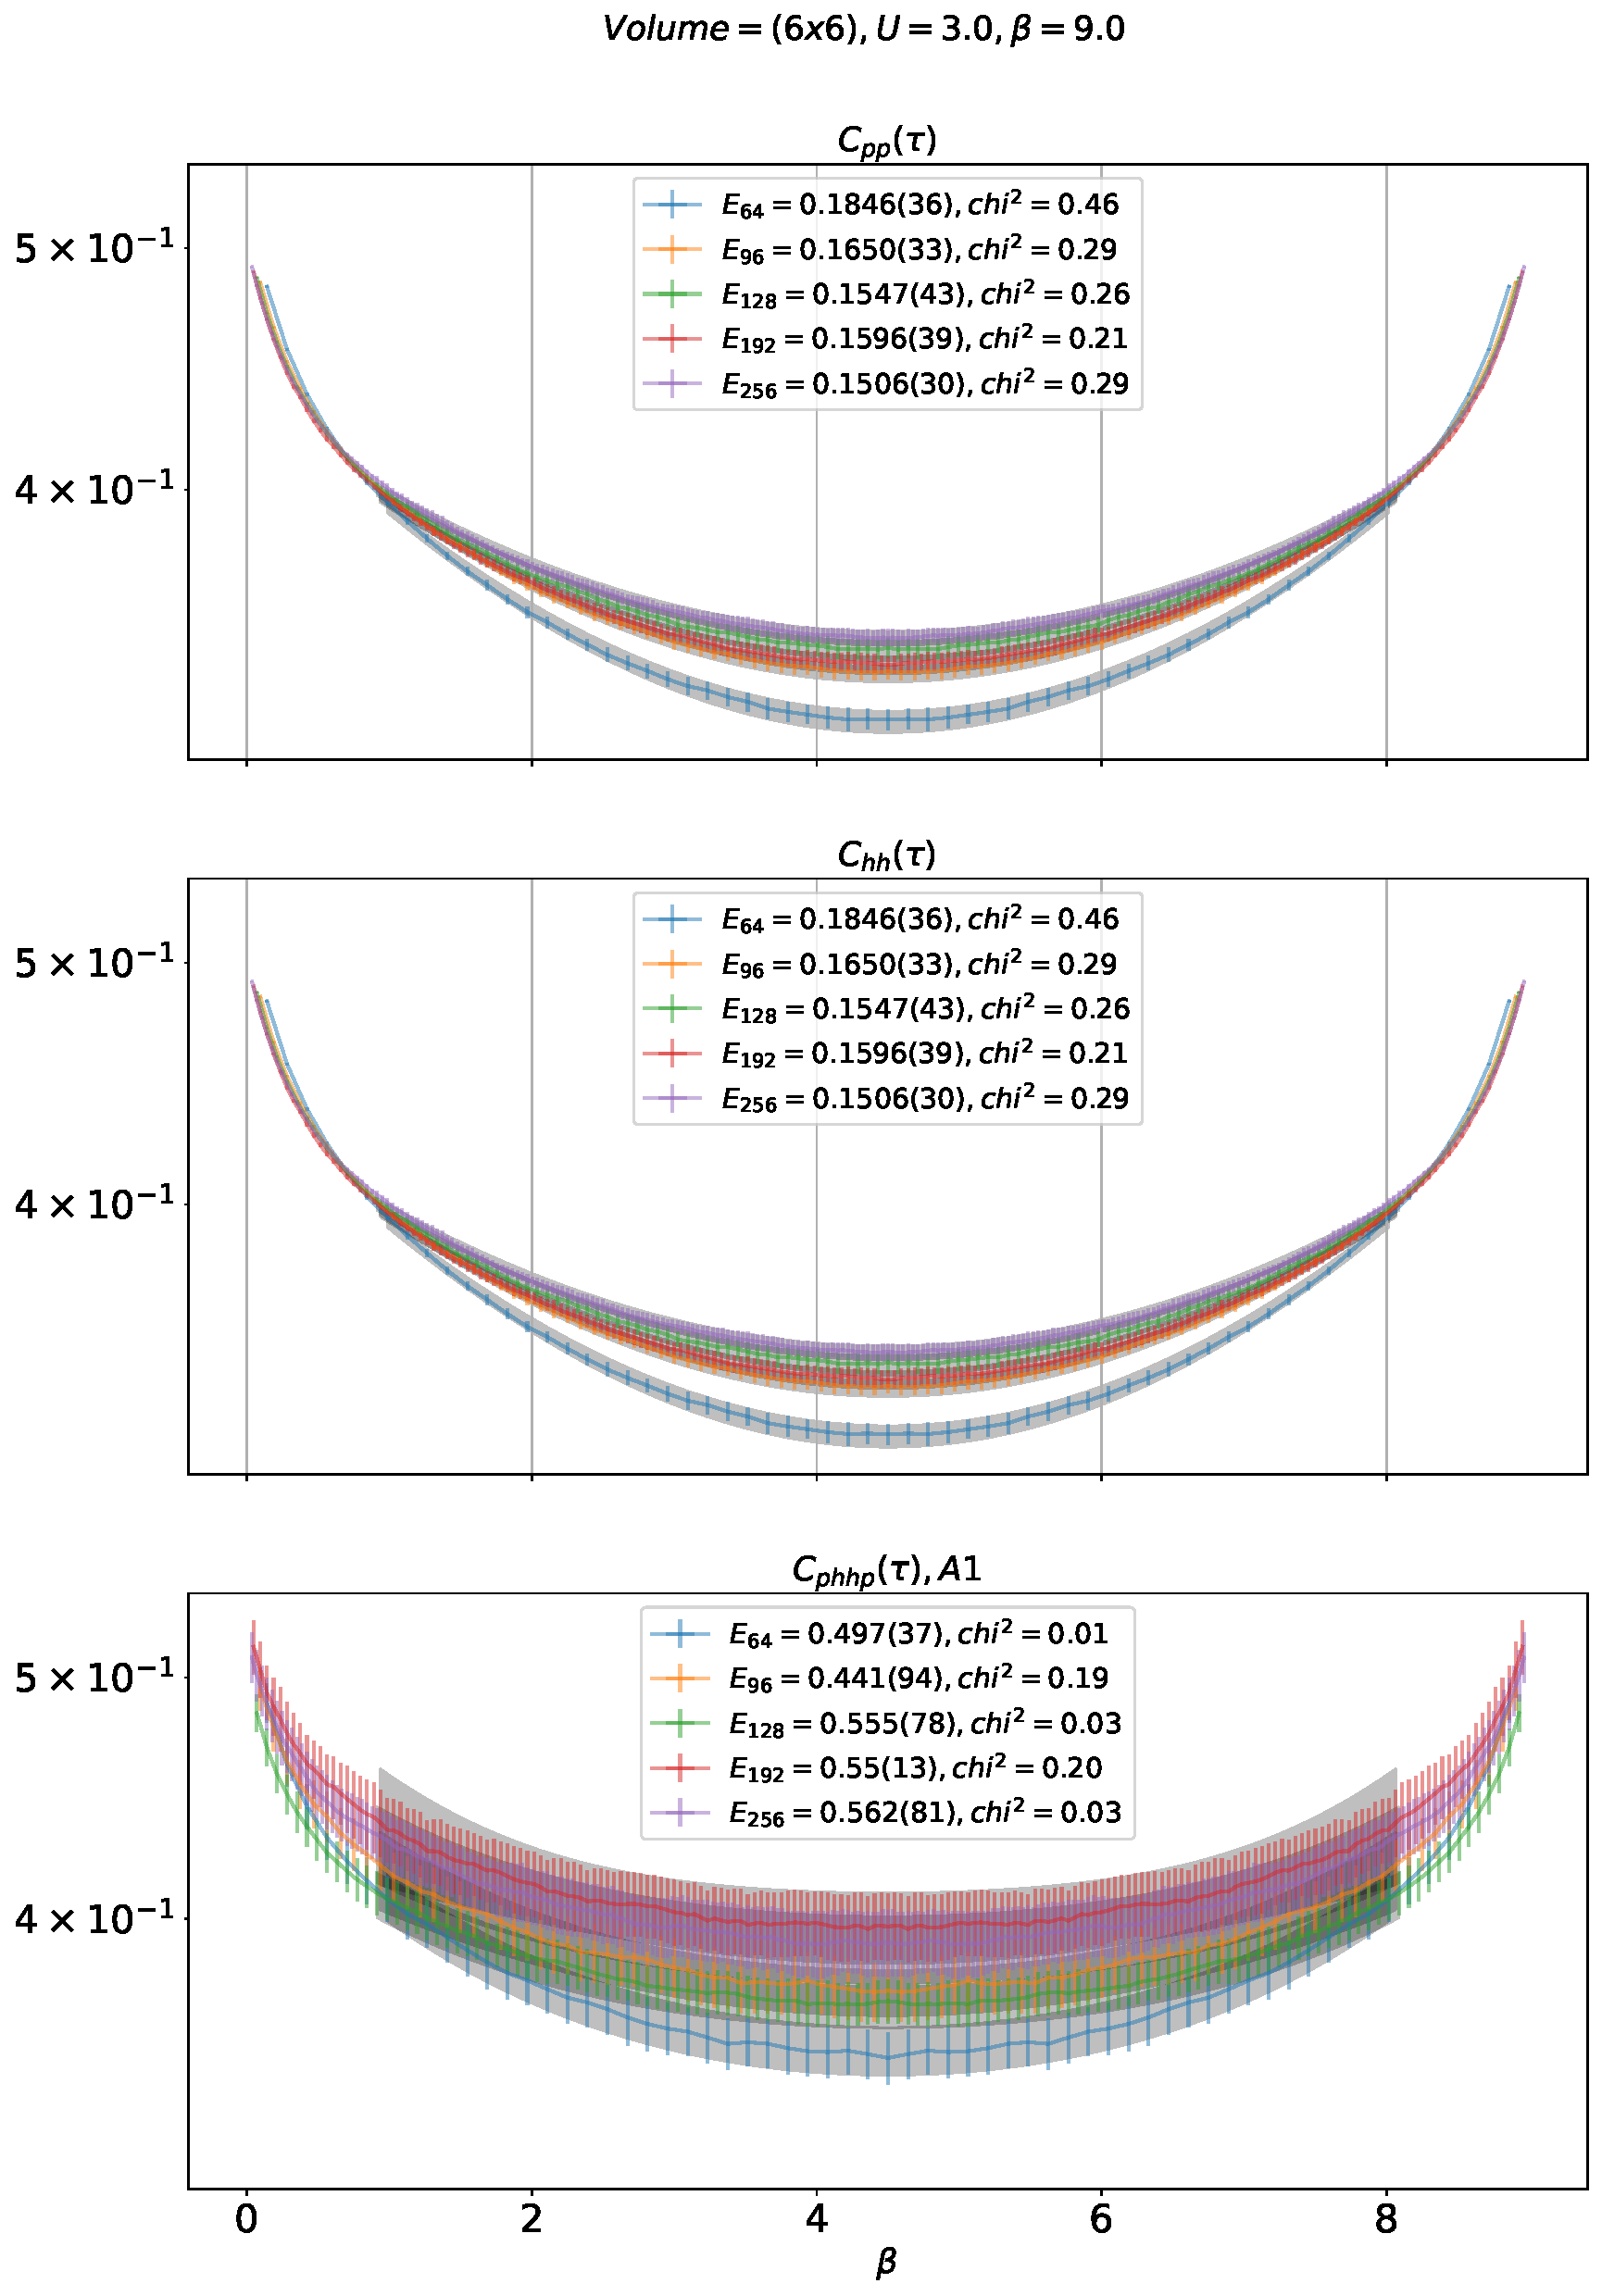
\includegraphics[width=\linewidth]{phhp-0-A1_6x6_U3.0_B9.0.pdf}
  \end{subfigure}%
  \begin{subfigure}{.5\textwidth}
    \centering
    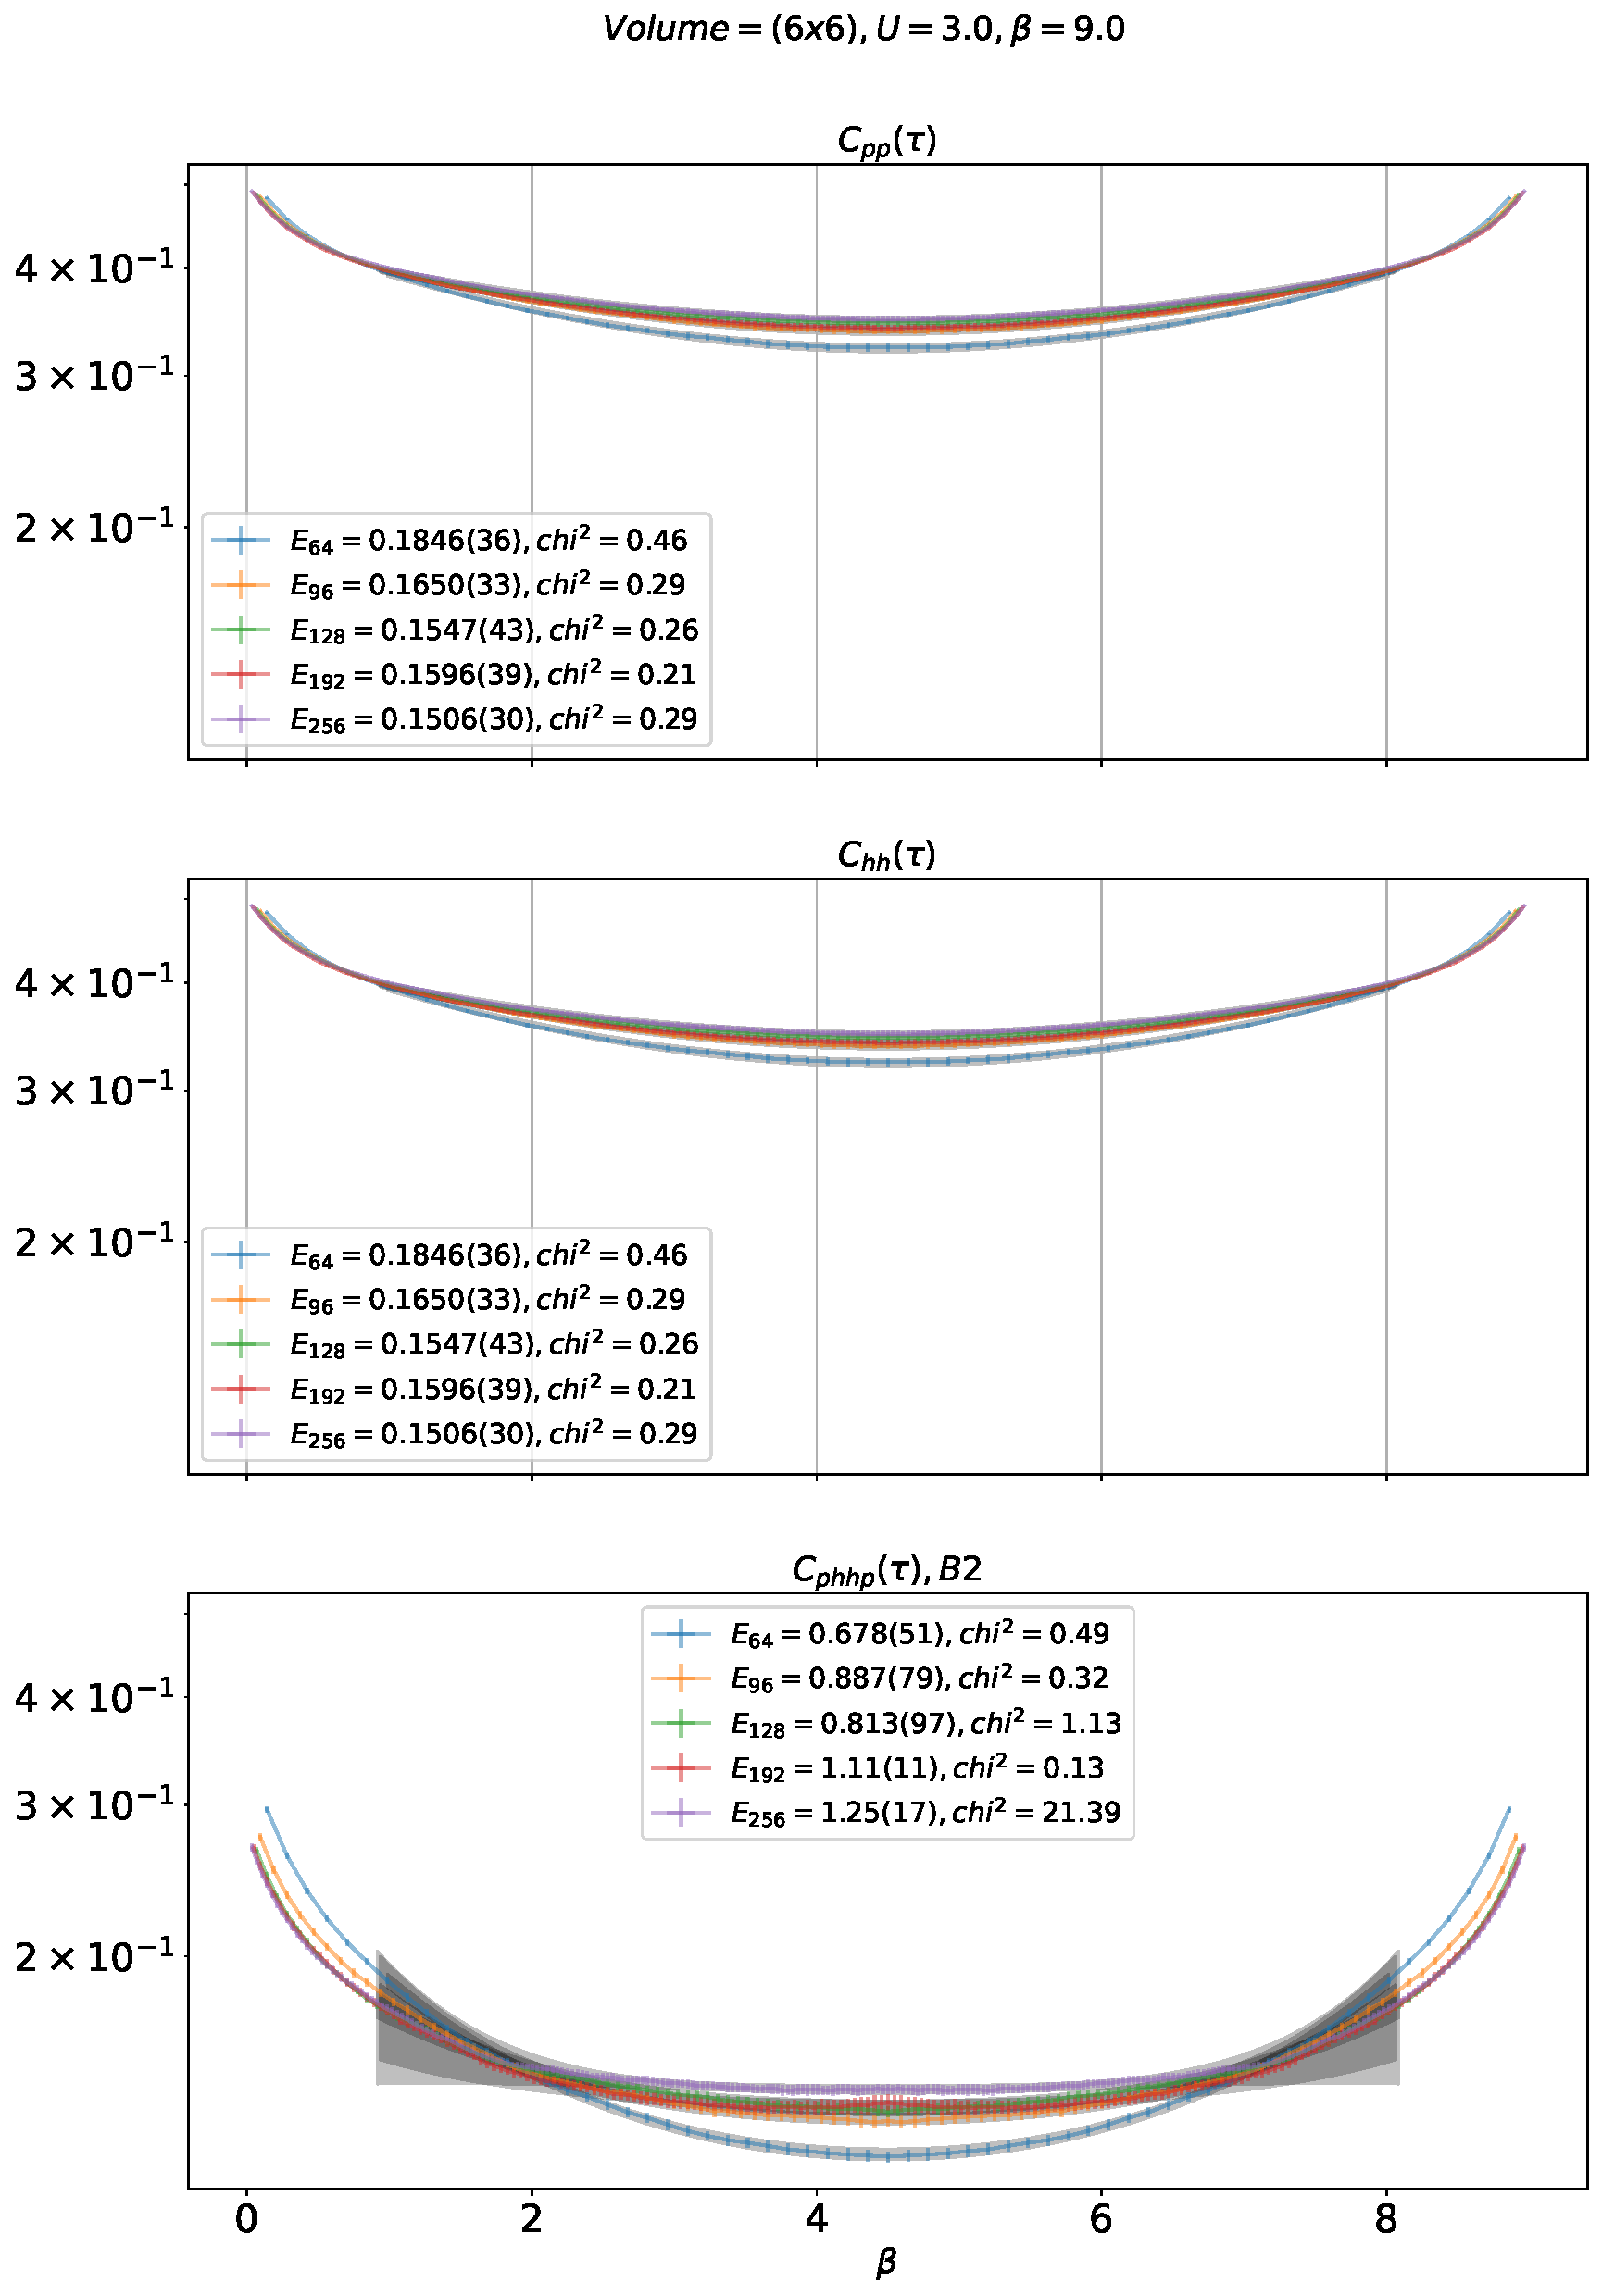
\includegraphics[width=\linewidth]{phhp-0-B2_6x6_U3.0_B9.0.pdf}
  \end{subfigure}
  \begin{subfigure}{.5\textwidth}
      \centering
      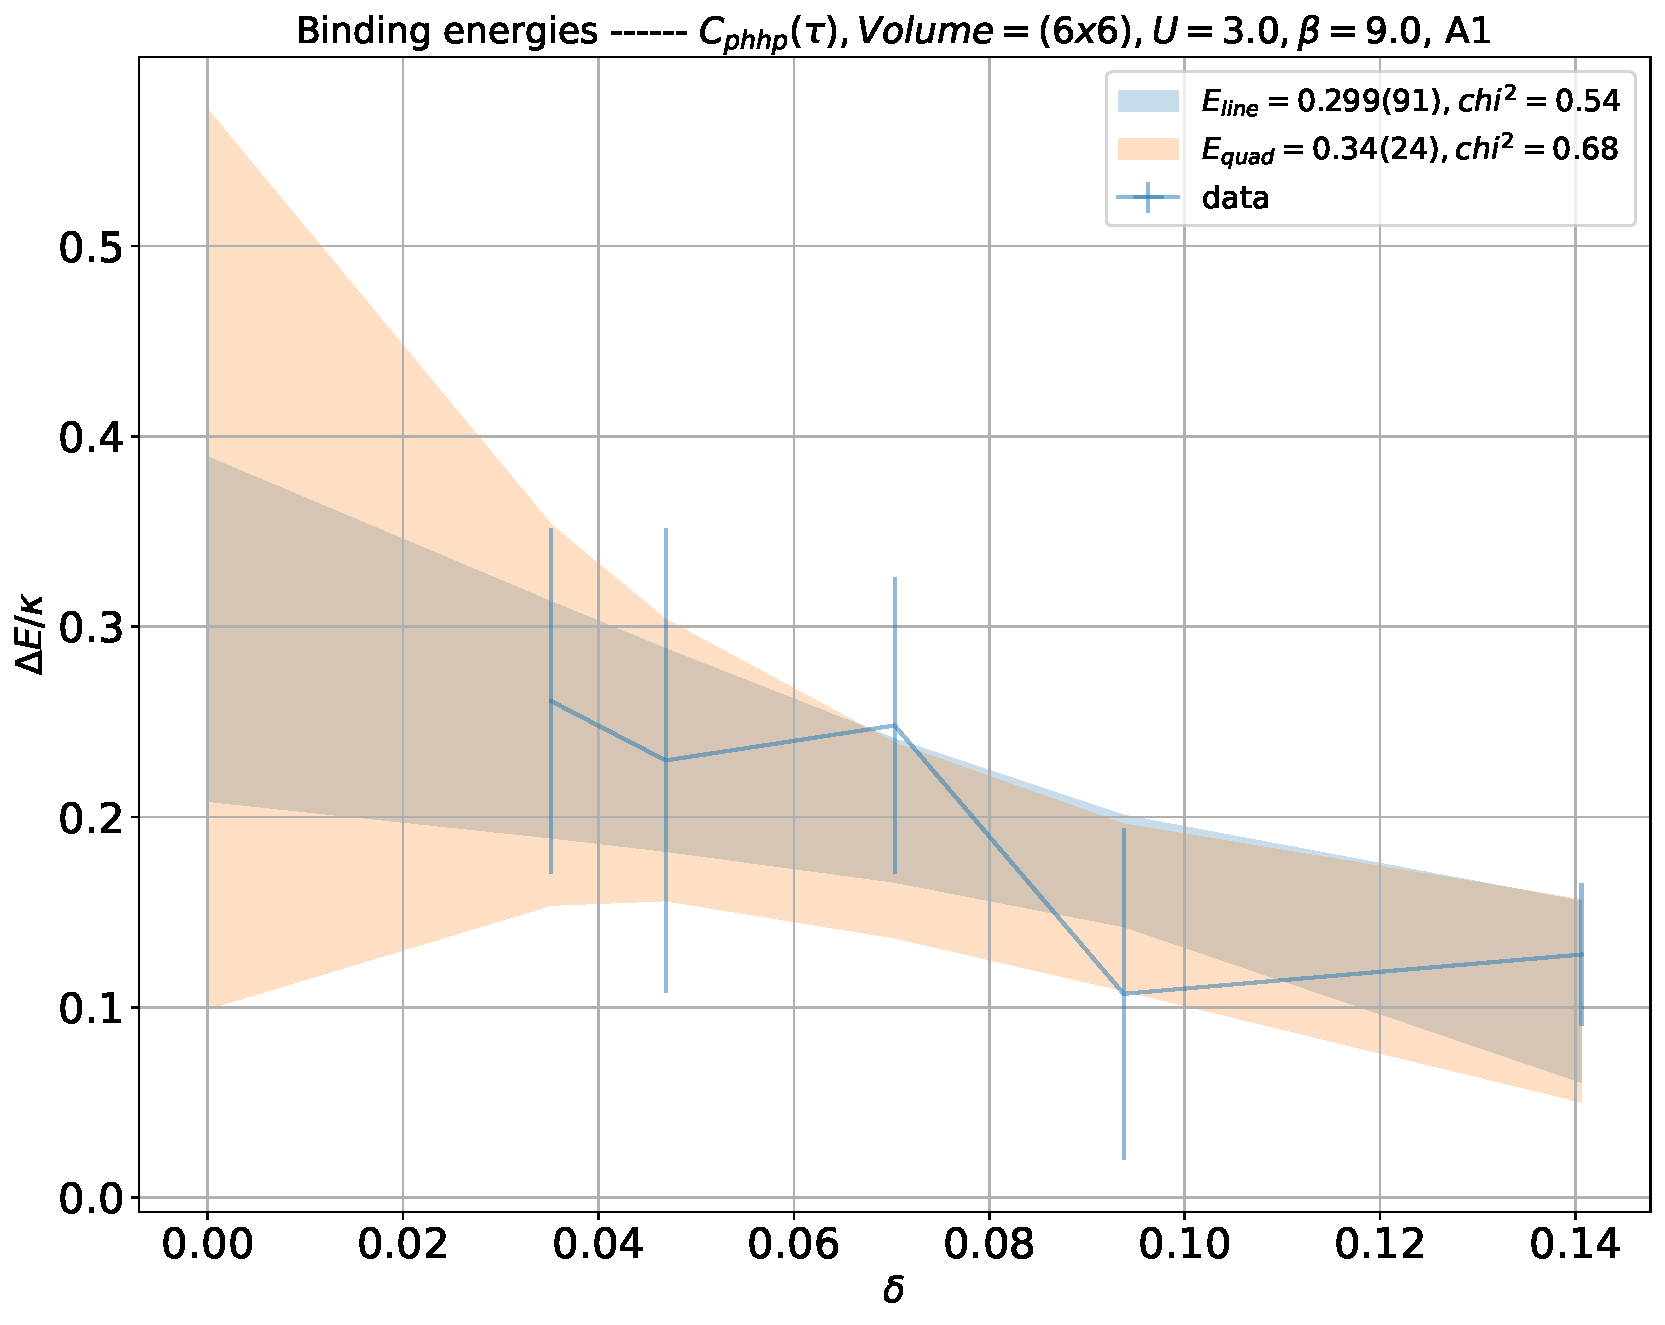
\includegraphics[width=\linewidth]{phhp-0-A1_6x6_U3.0_B9.0_cont.pdf}
  \end{subfigure}
  \begin{subfigure}{.5\textwidth}
      \centering
      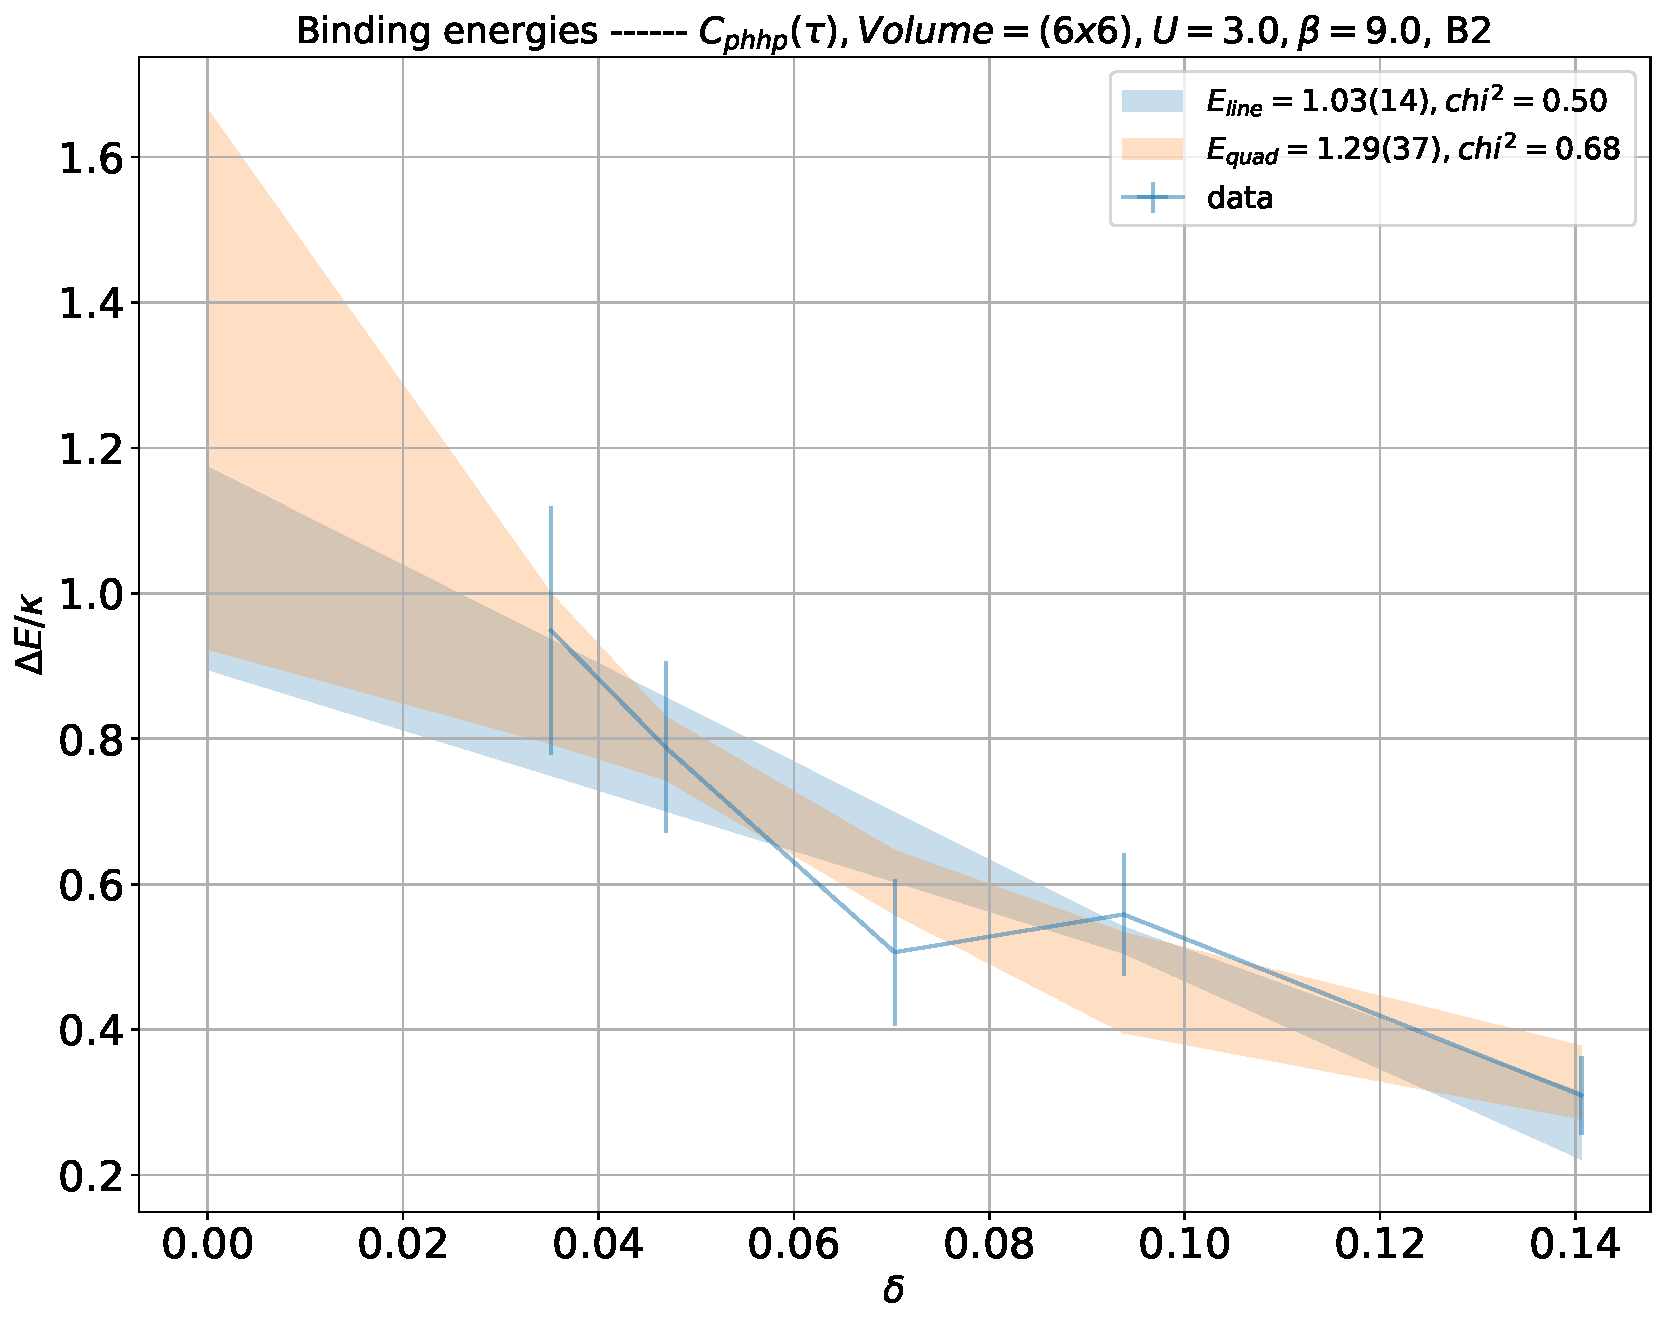
\includegraphics[width=\linewidth]{phhp-0-B2_6x6_U3.0_B9.0_cont.pdf}
  \end{subfigure}
  \caption{Binding energy extraction of the particle-hole pair at both irreducible representations, where we fit one- and two-body correlators for every $N_t$. This is followed by fitting a linear and a quadratic functions to the $\Delta E_{N_t}$ in order to extrapolate to the continuum limit ($N_t\to\infty$).}
  \label{fig:fig11}
\end{figure}

\begin{figure}
  \begin{subfigure}{.5\textwidth}
    \centering
    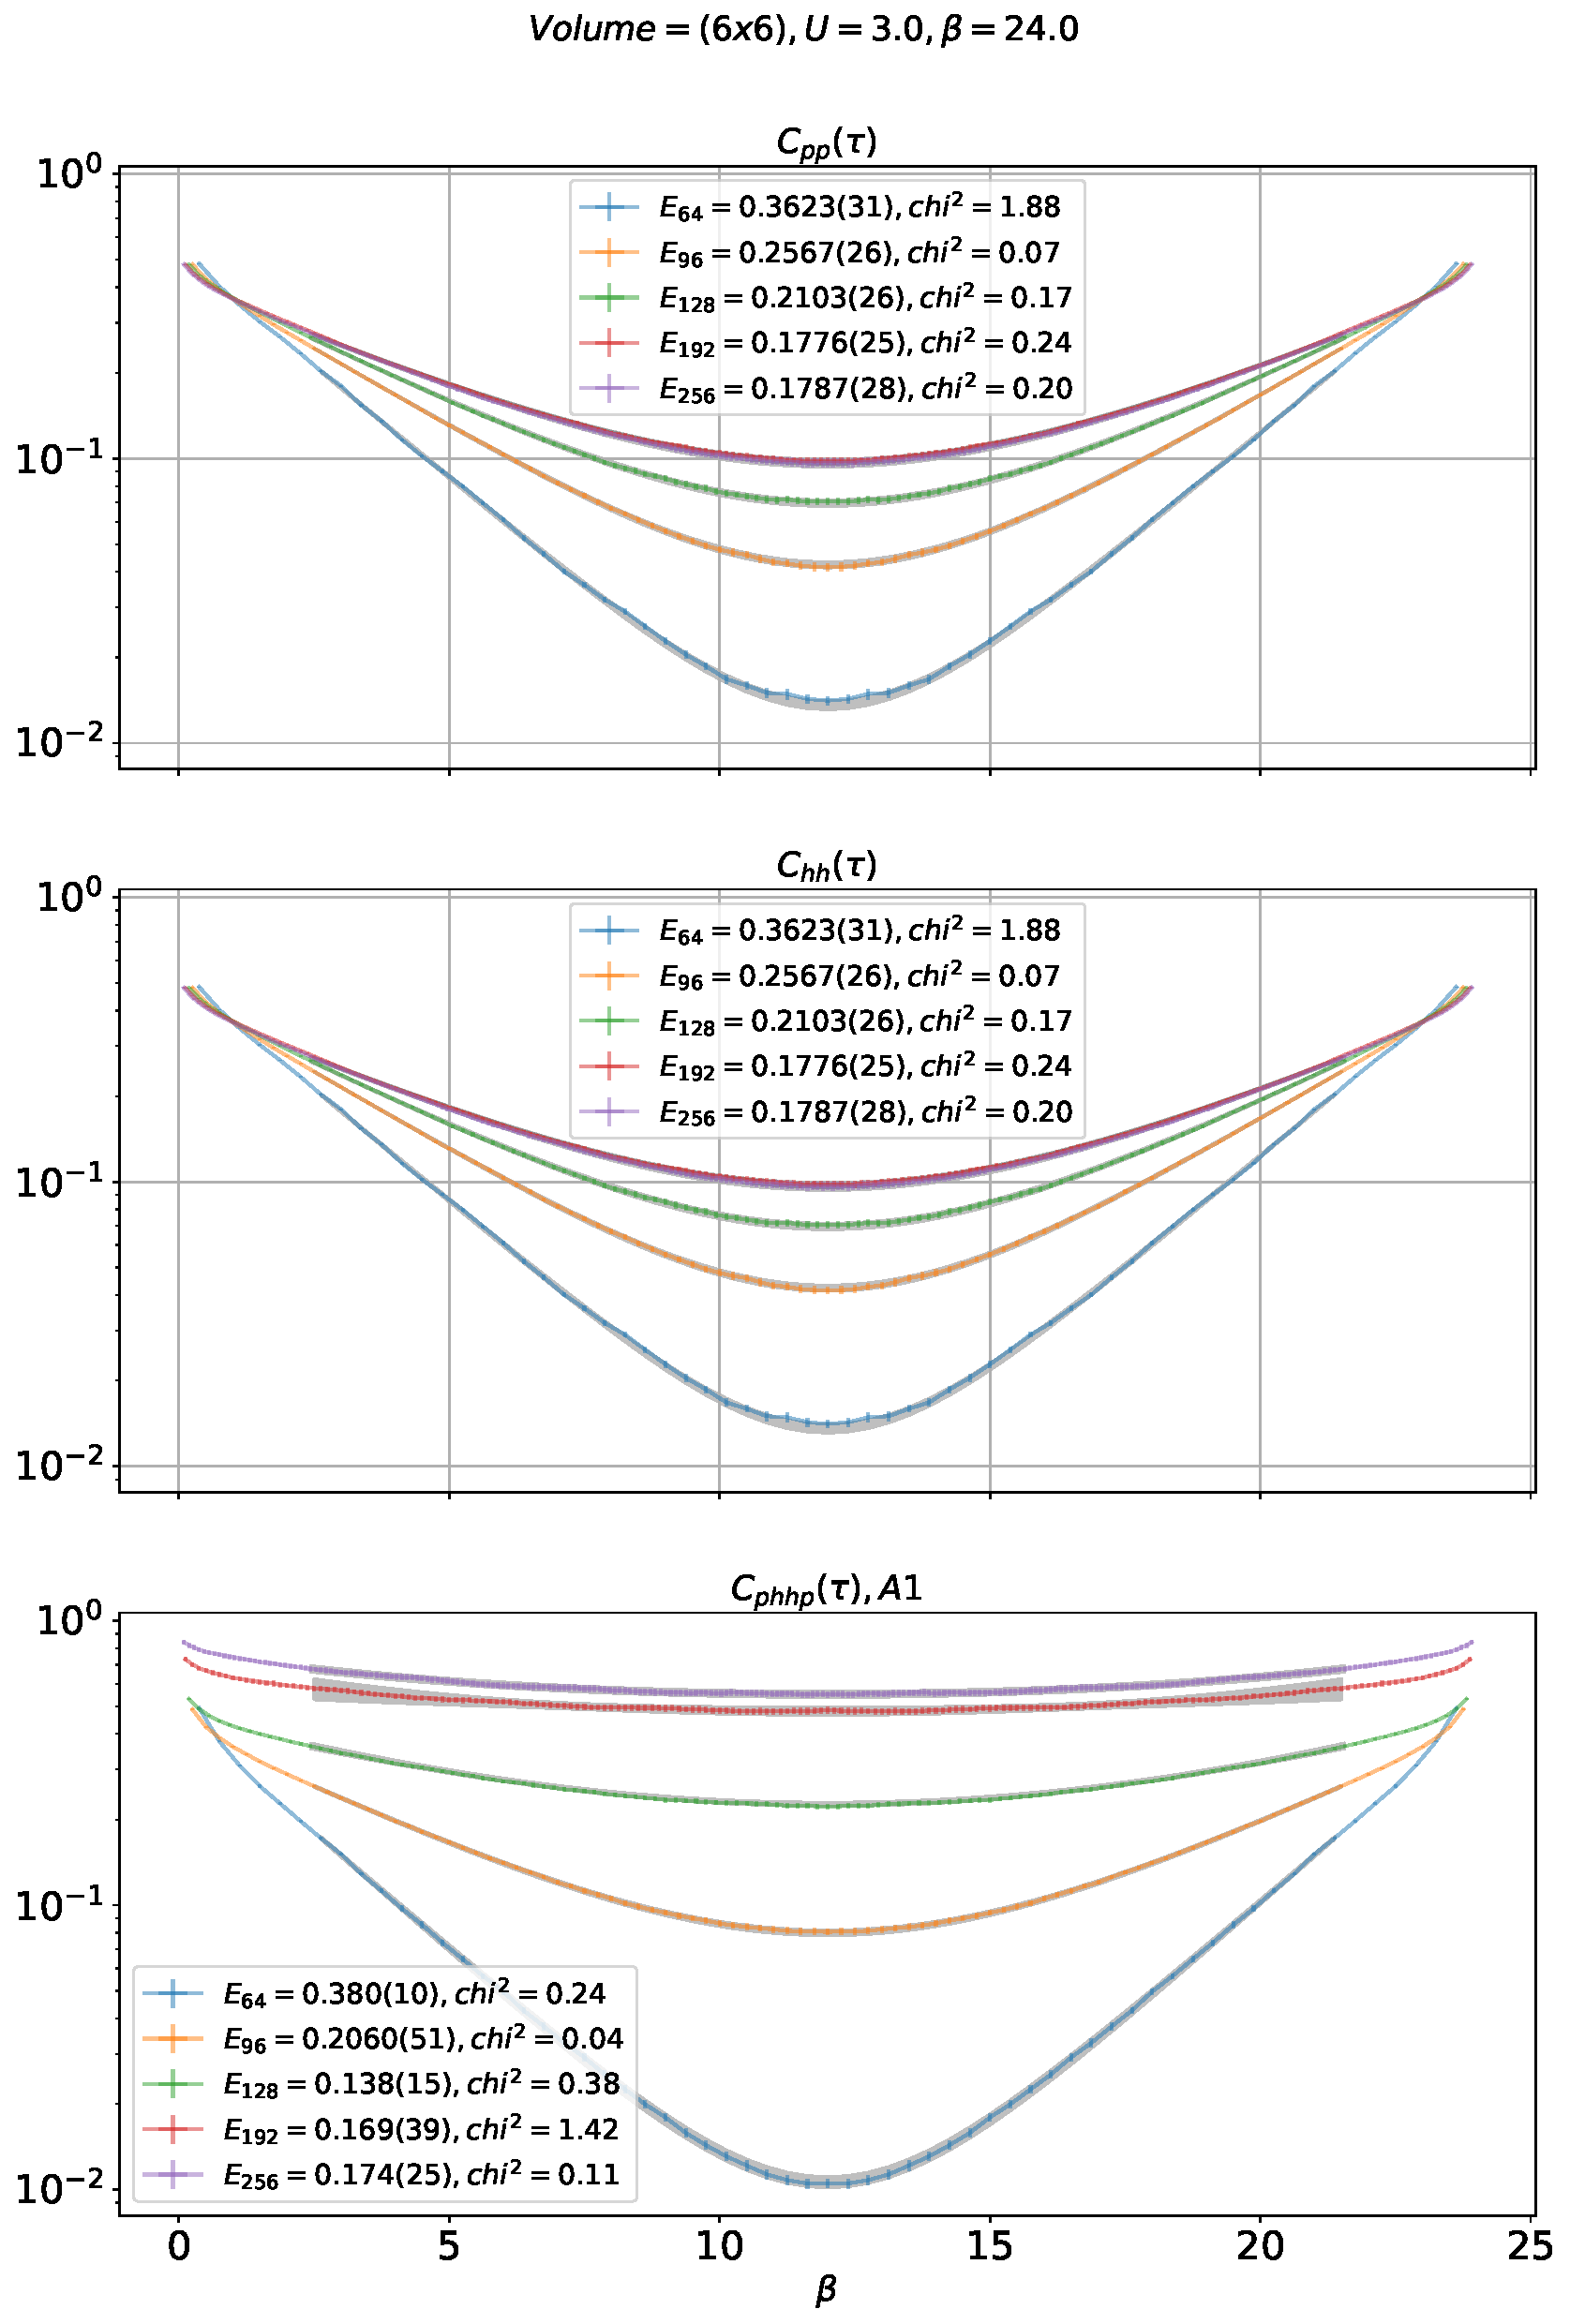
\includegraphics[width=\linewidth]{phhp-0-A1_6x6_U3.0_B24.0.pdf}
  \end{subfigure}%
  \begin{subfigure}{.5\textwidth}
    \centering
    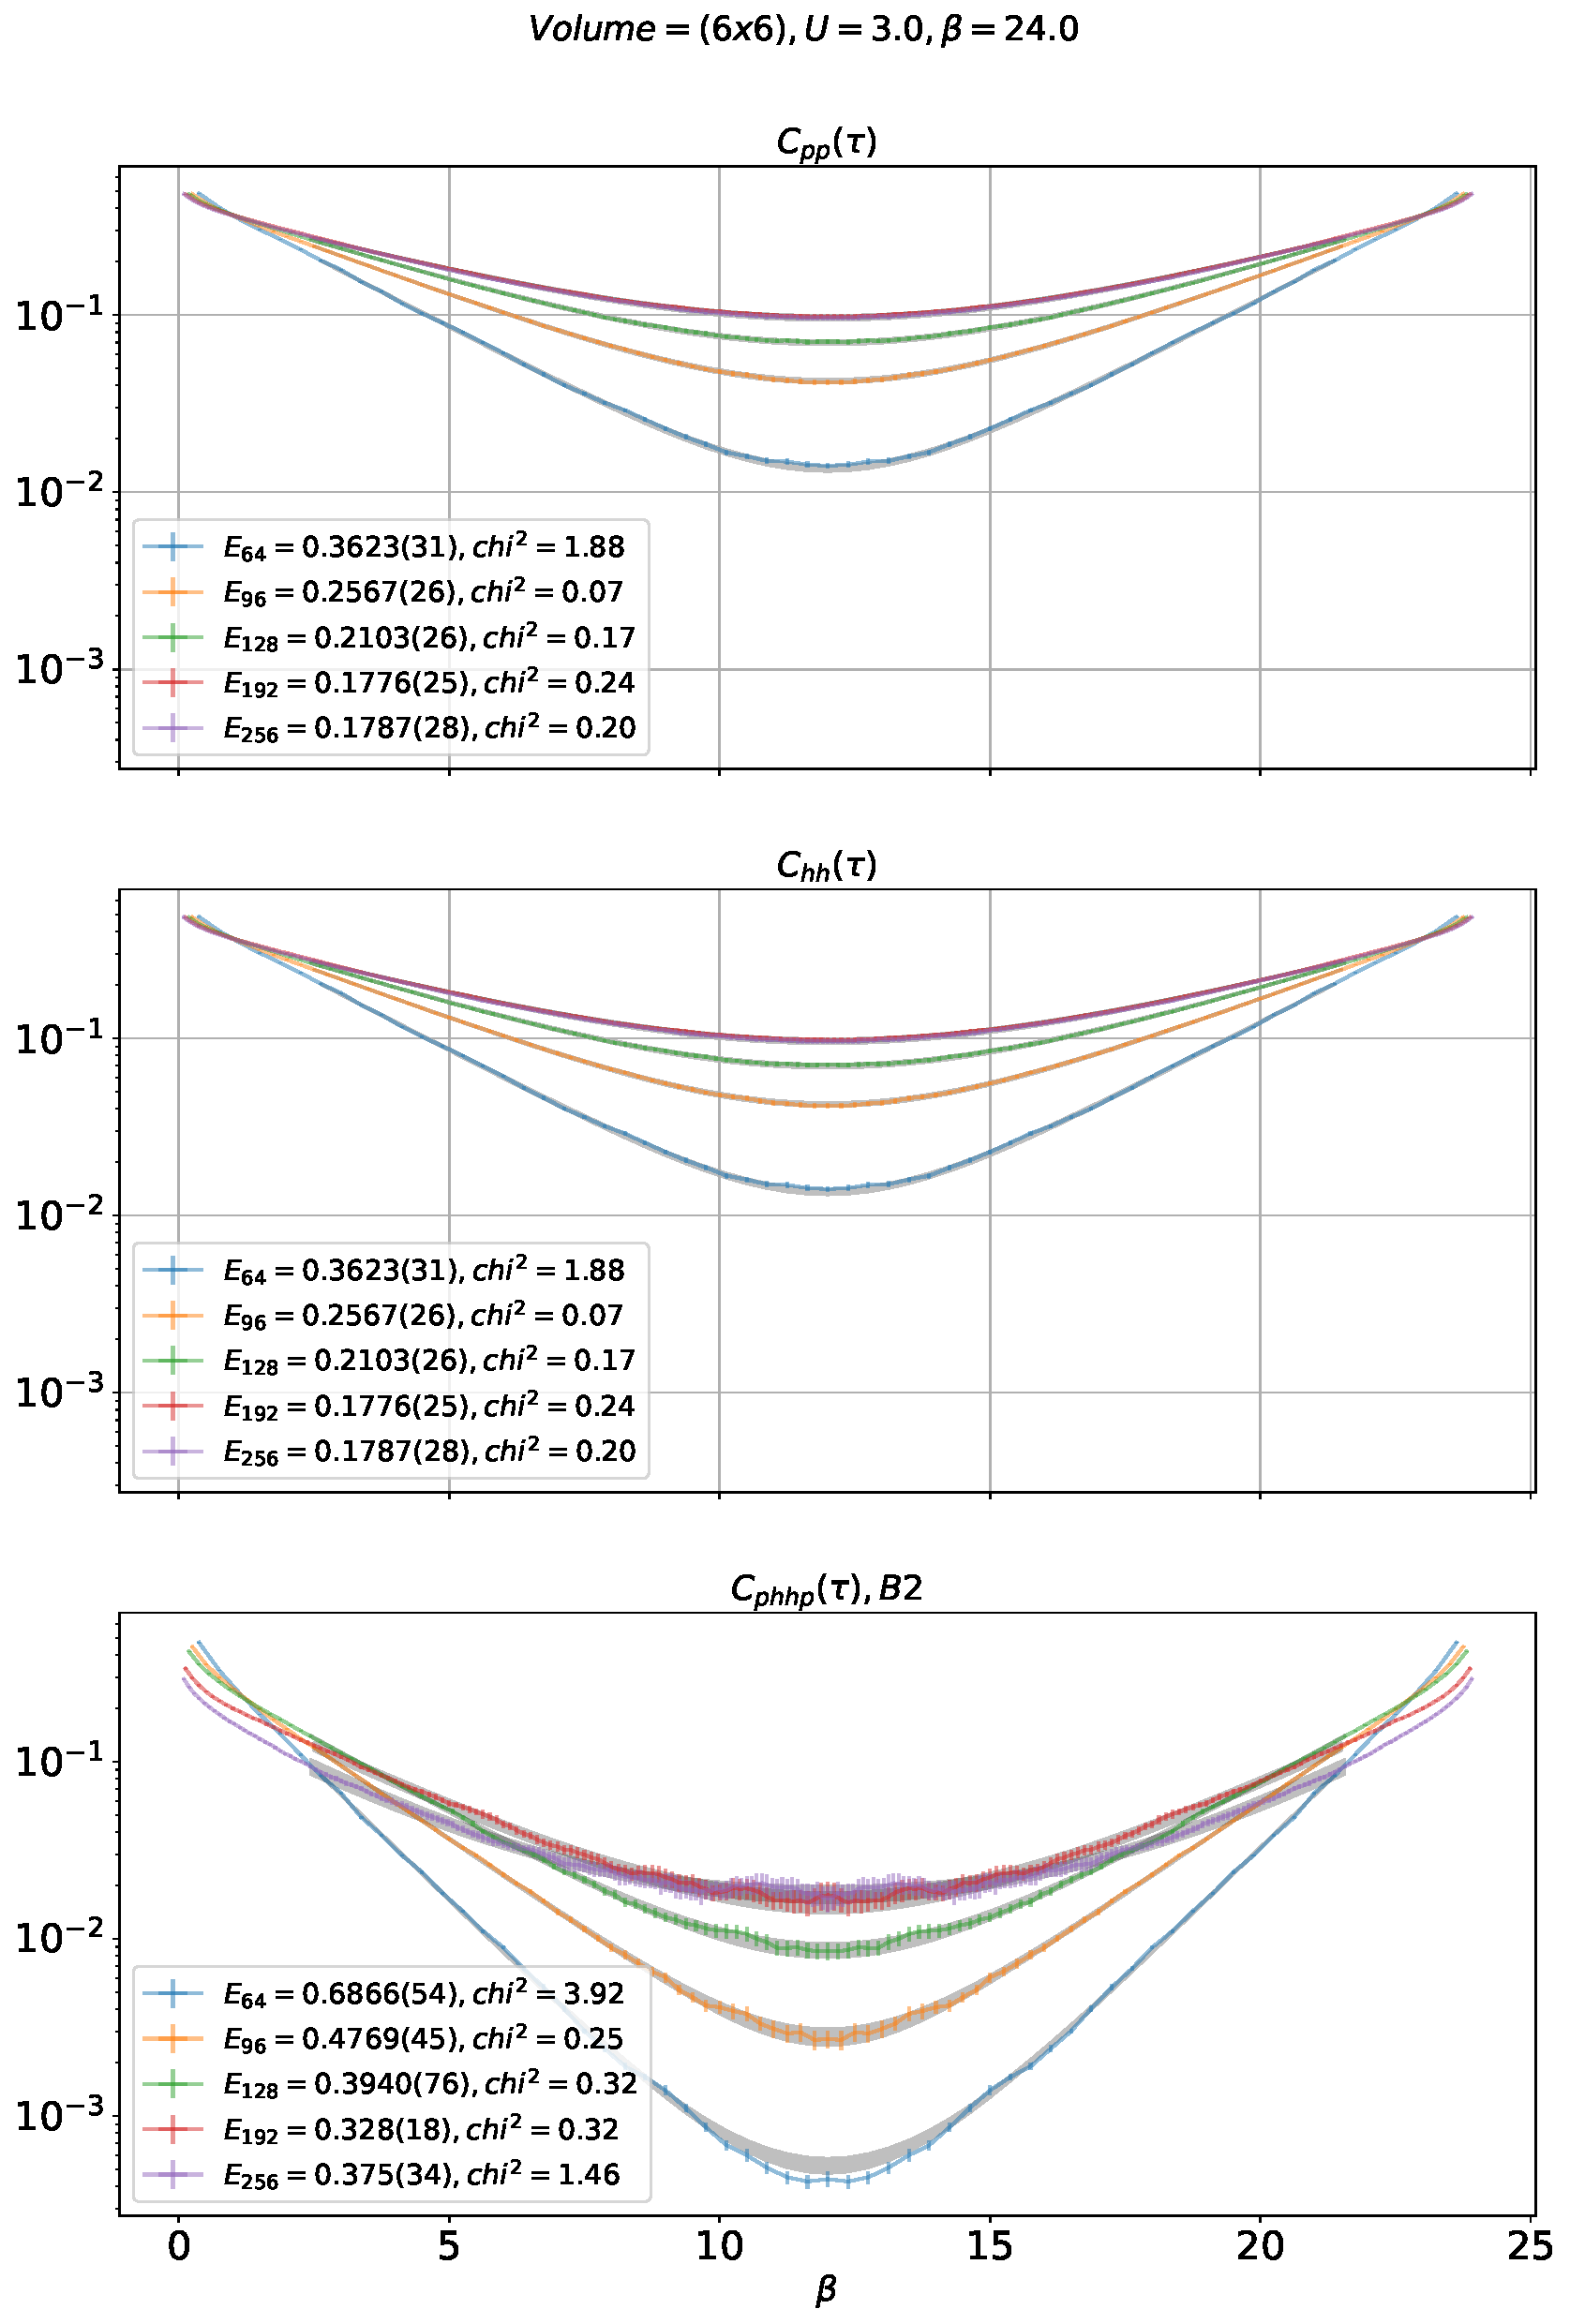
\includegraphics[width=\linewidth]{phhp-0-B2_6x6_U3.0_B24.0.pdf}
  \end{subfigure}
  \begin{subfigure}{.5\textwidth}
      \centering
      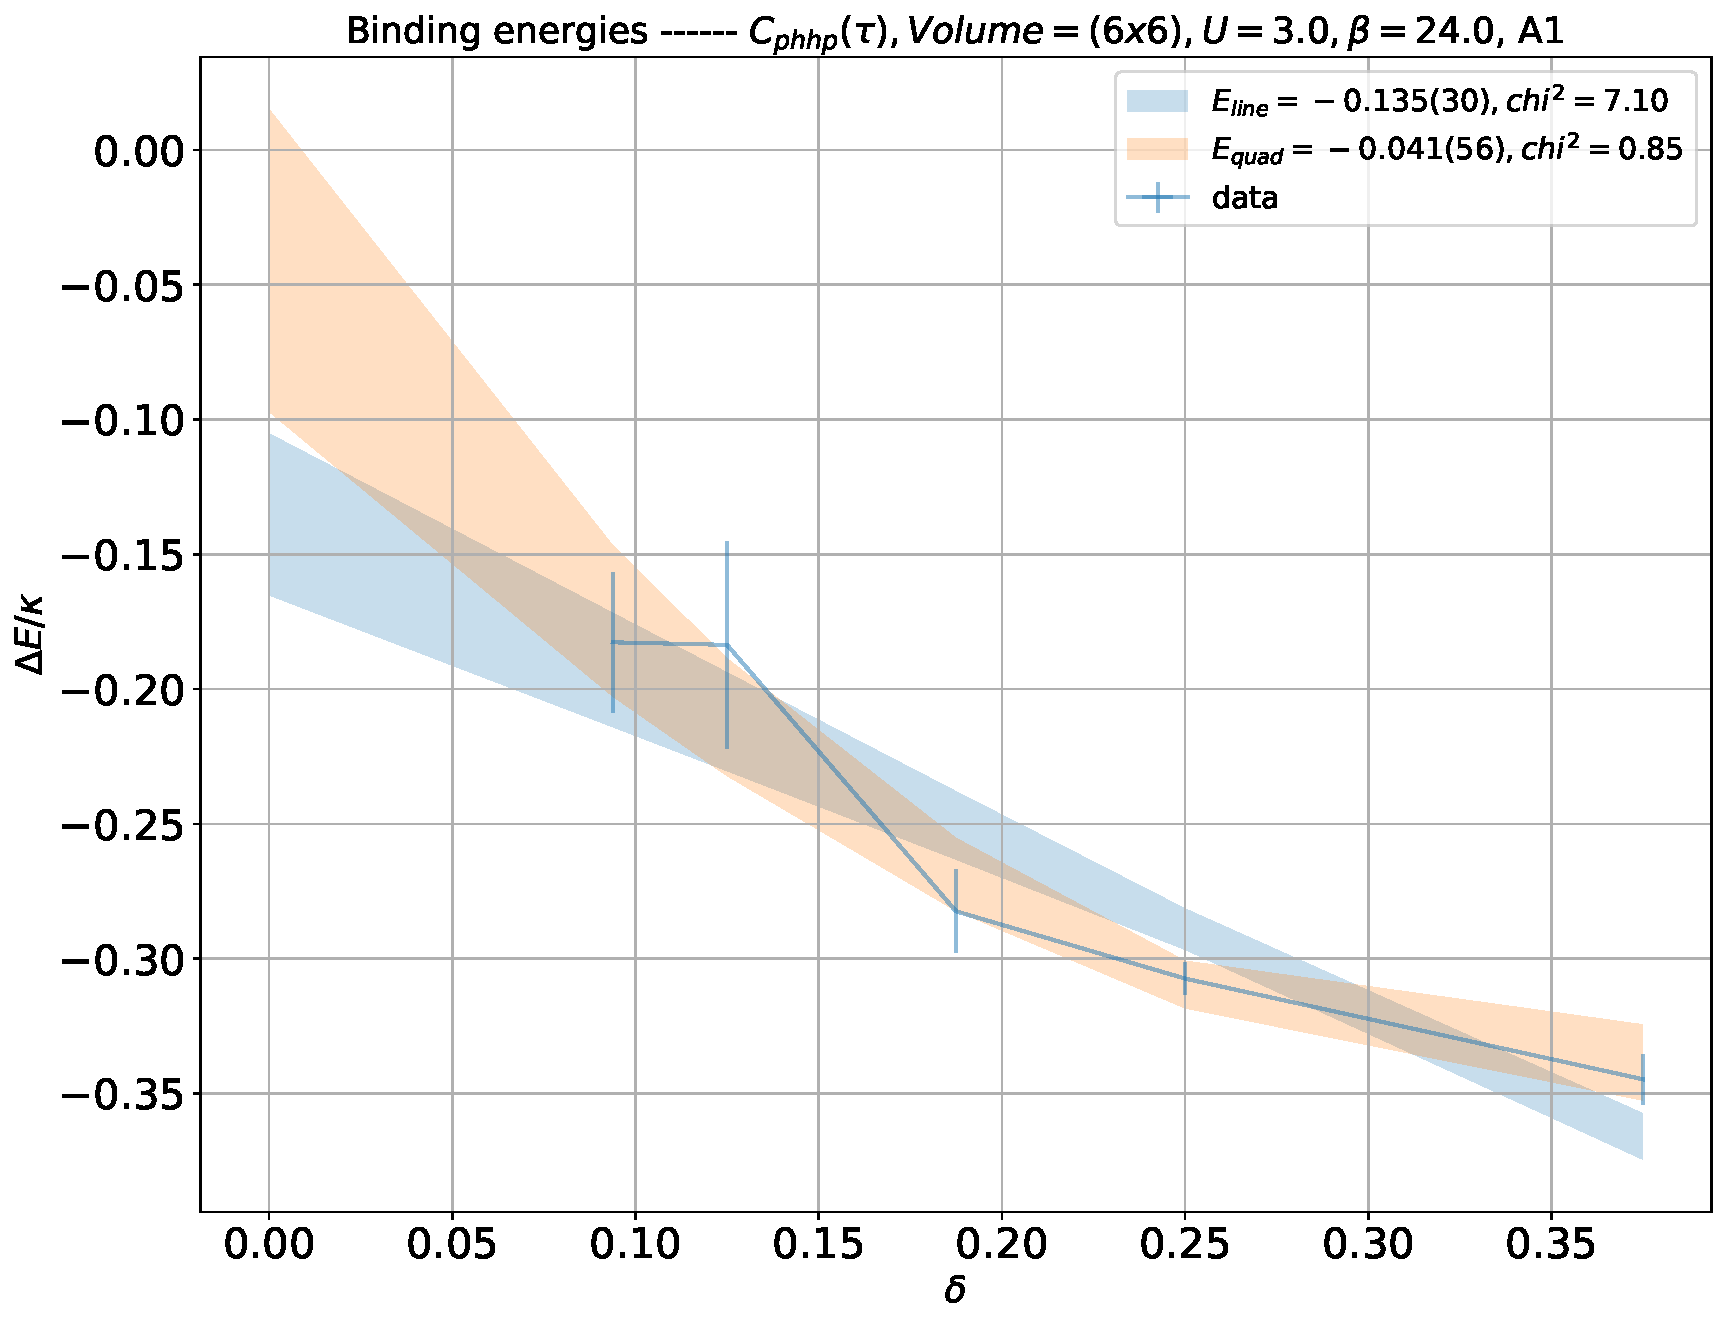
\includegraphics[width=\linewidth]{phhp-0-A1_6x6_U3.0_B24.0_cont.pdf}
  \end{subfigure}
  \begin{subfigure}{.5\textwidth}
      \centering
      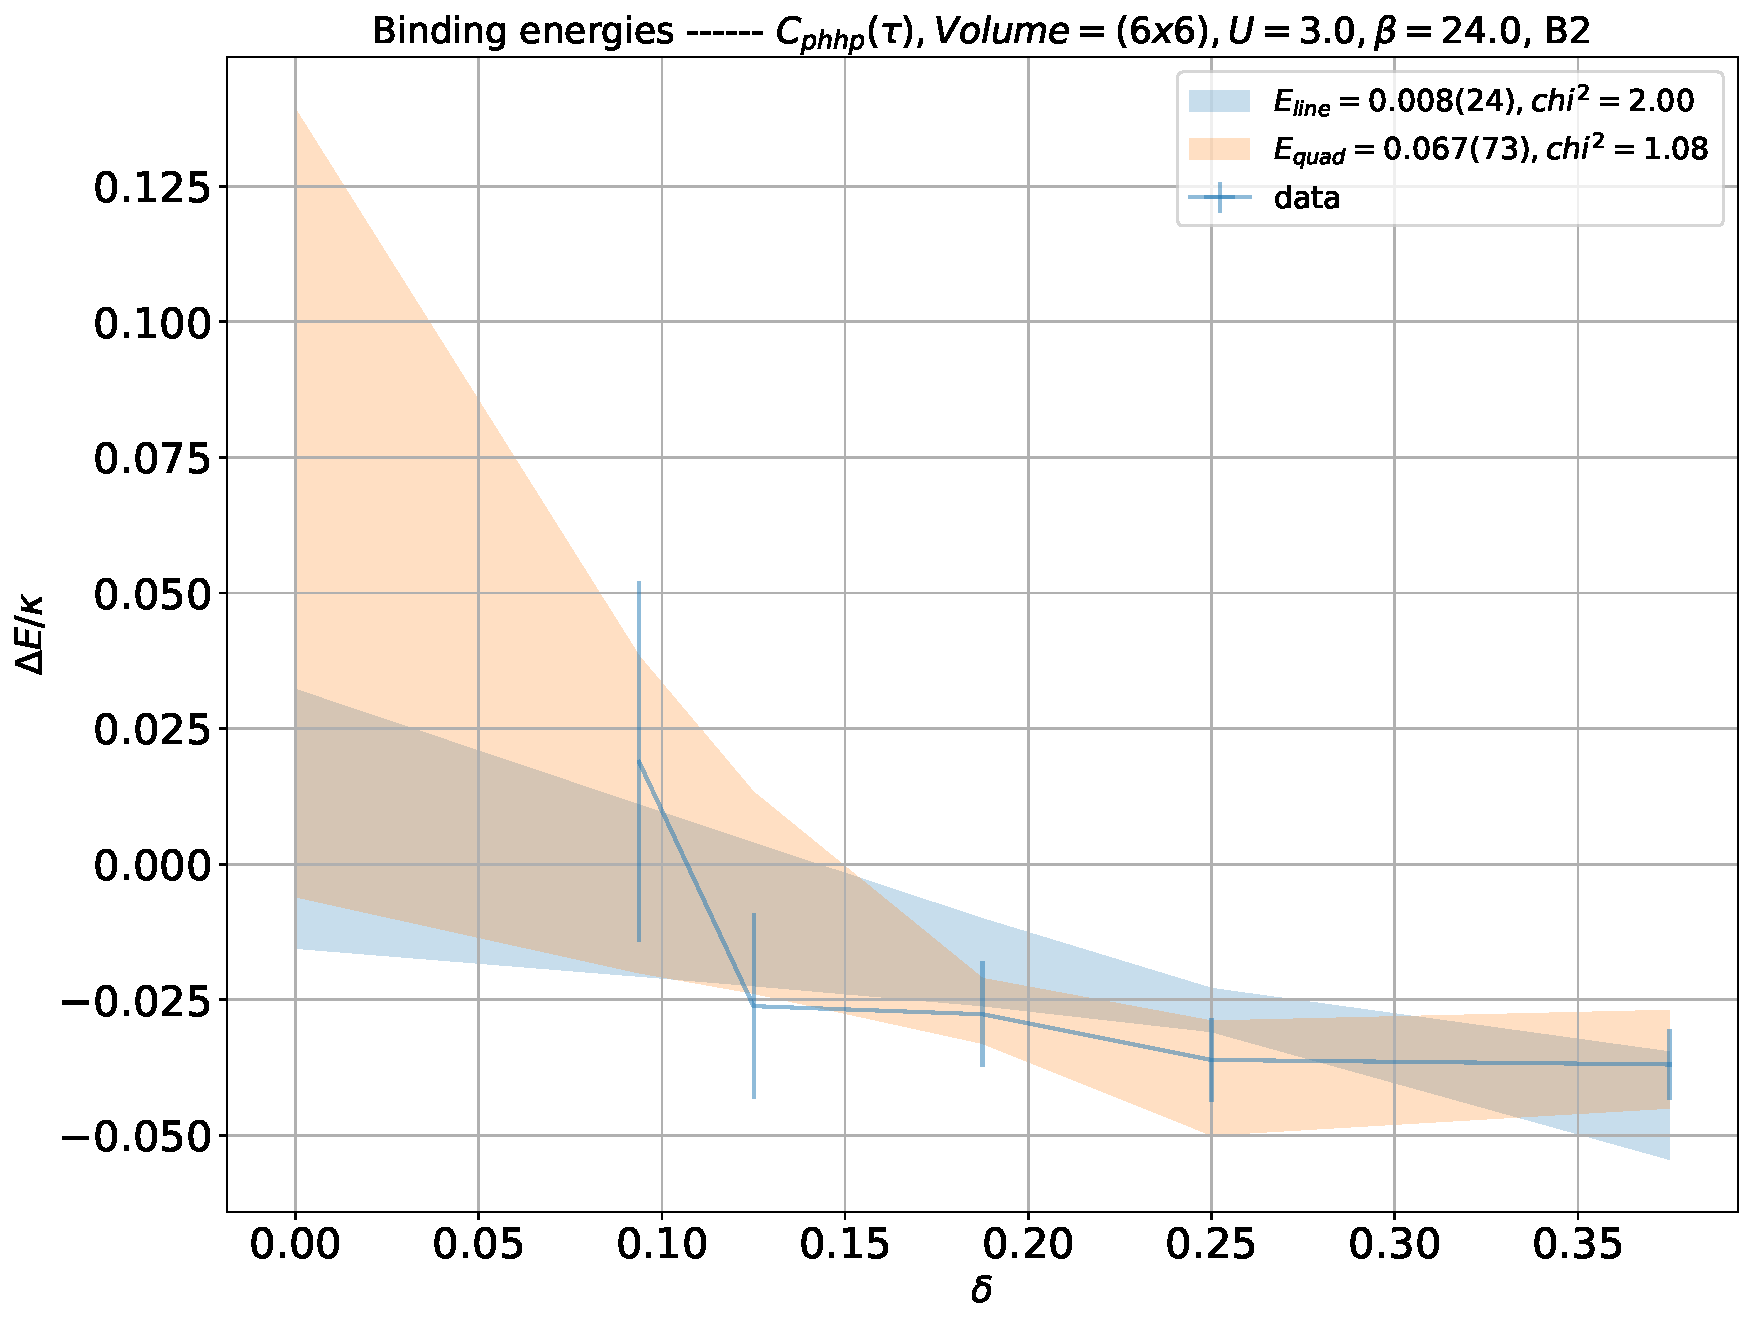
\includegraphics[width=\linewidth]{phhp-0-B2_6x6_U3.0_B24.0_cont.pdf}
  \end{subfigure}
  \caption{Binding energy extraction of the particle-hole pair at both irreducible representations, where we fit one- and two-body correlators for every $N_t$. This is followed by fitting a linear and a quadratic functions to the $\Delta E_{N_t}$ in order to extrapolate to the continuum limit ($N_t\to\infty$).}
  \label{fig:fig12}
\end{figure}

\begin{figure}
  \begin{subfigure}{.5\textwidth}
    \centering
    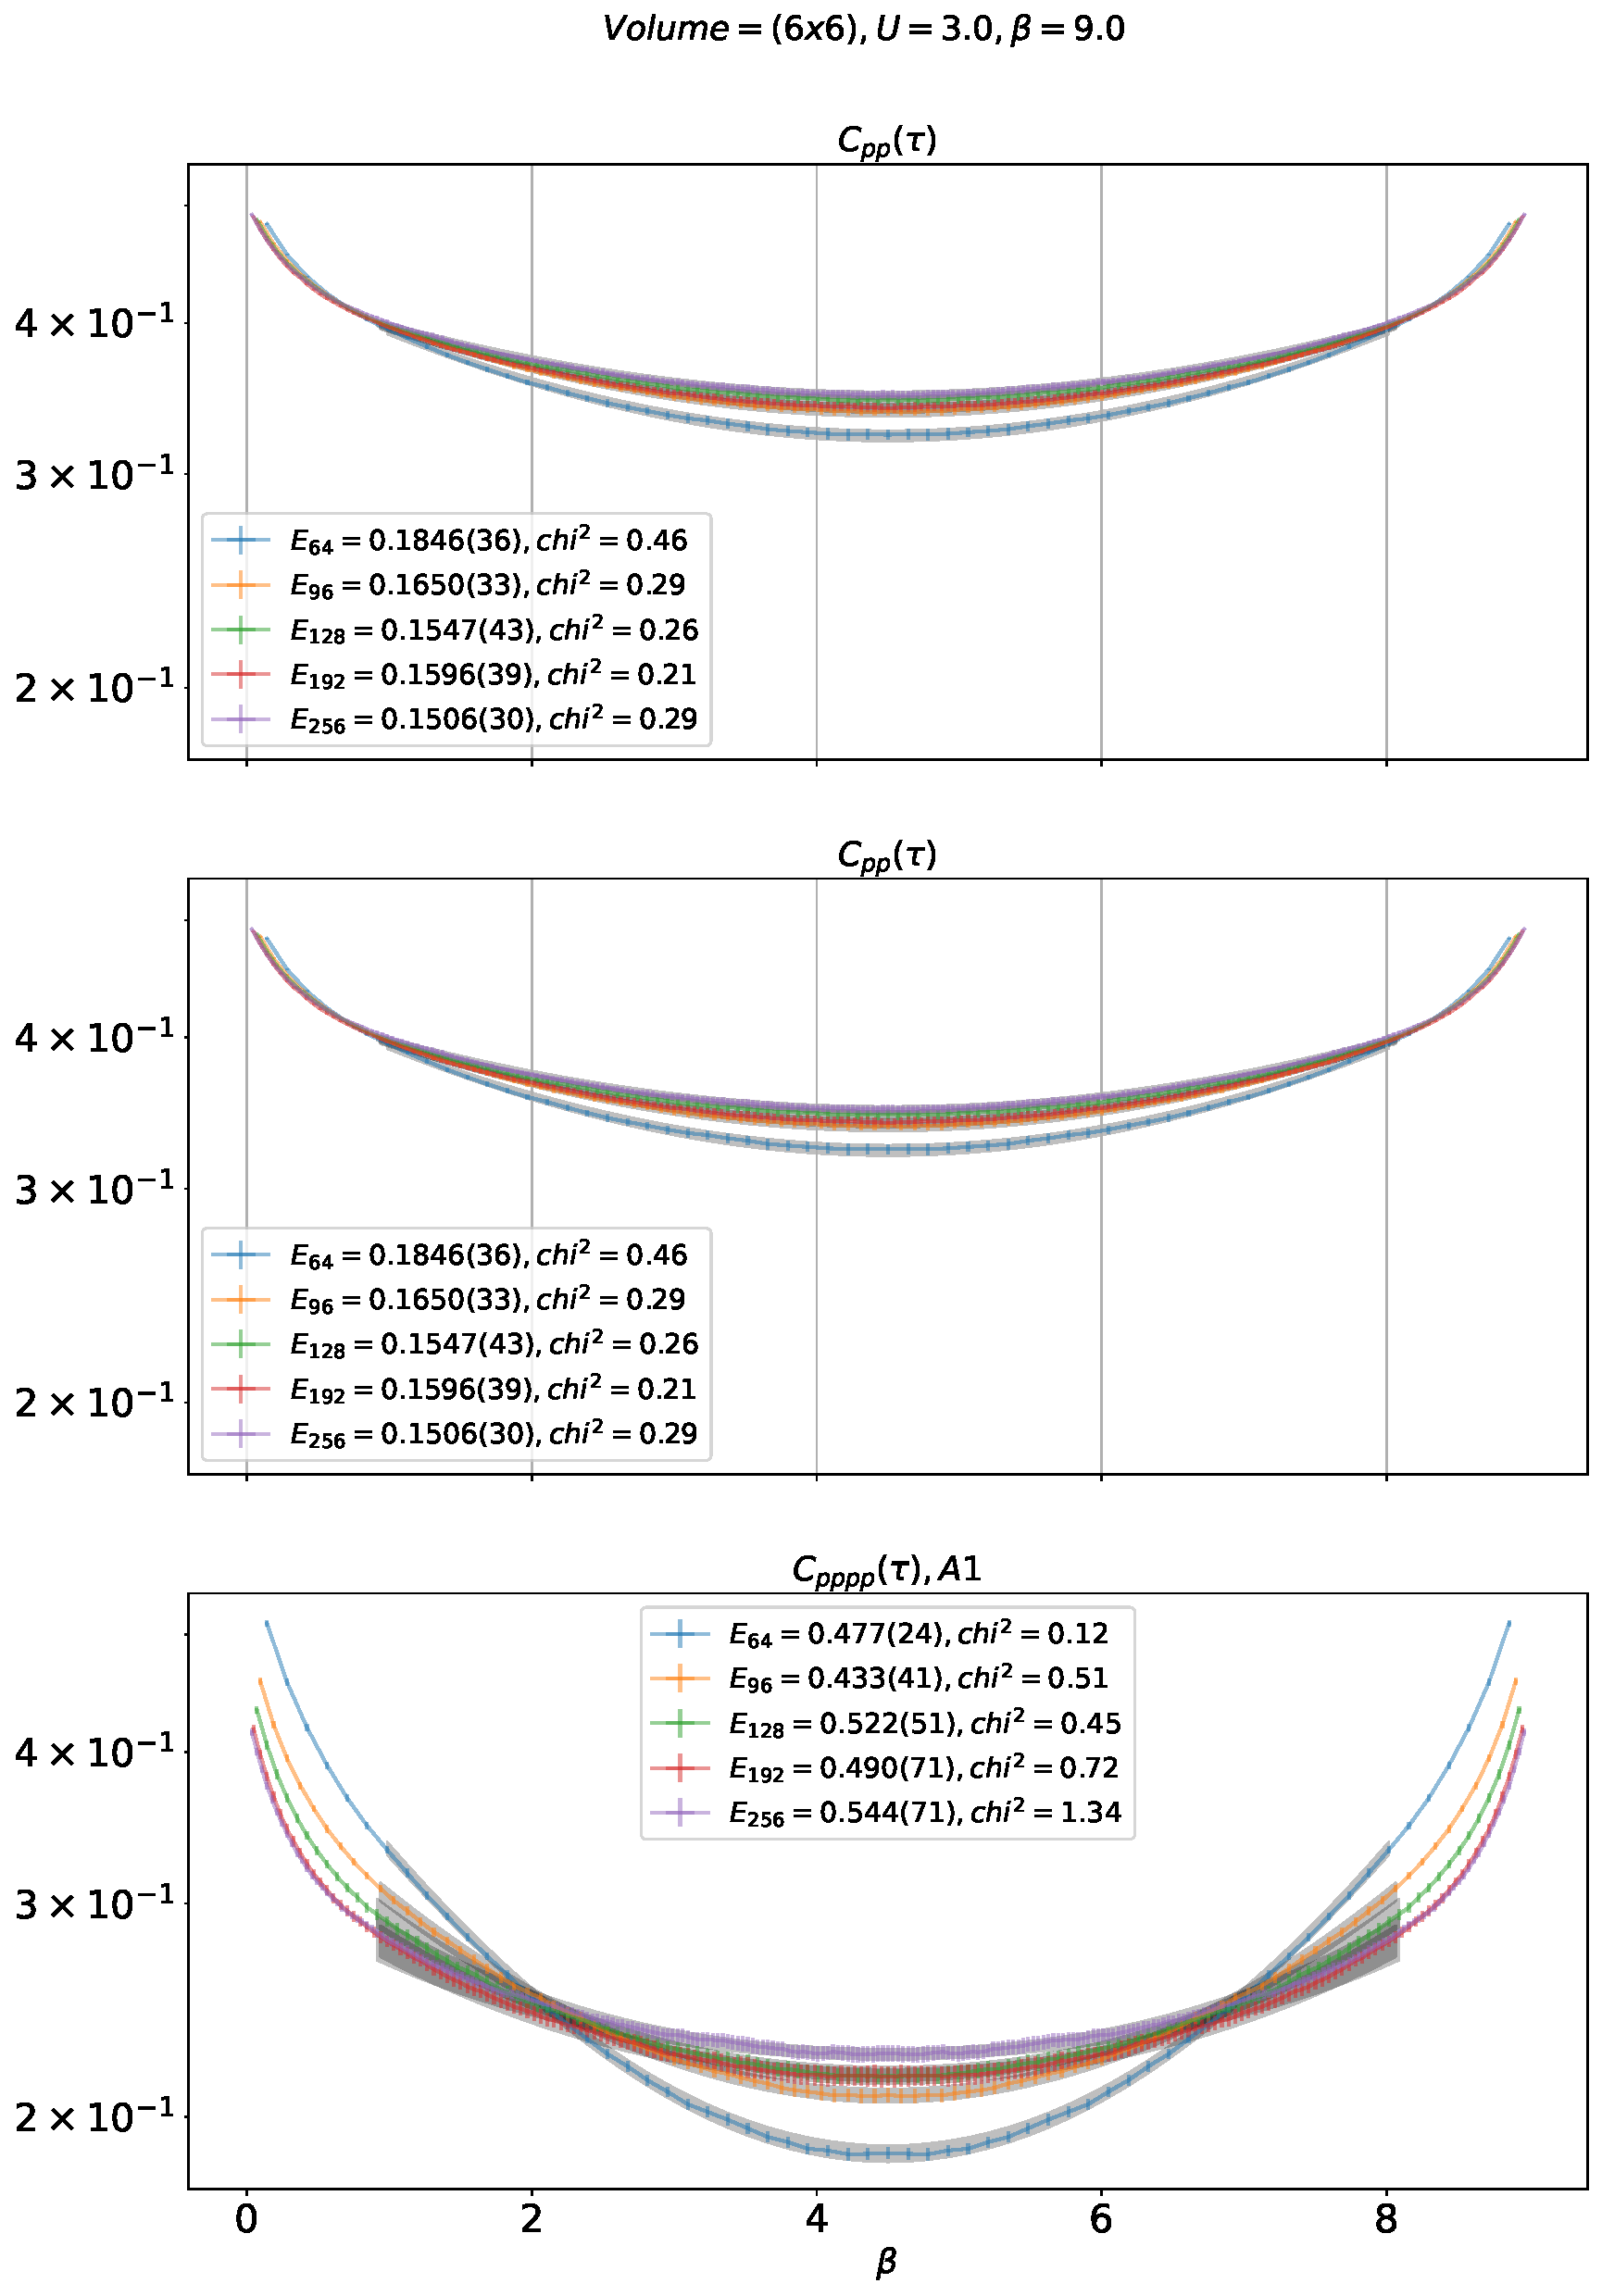
\includegraphics[width=\linewidth]{pppp-0-A1_6x6_U3.0_B9.0.pdf}
  \end{subfigure}%
  \begin{subfigure}{.5\textwidth}
    \centering
    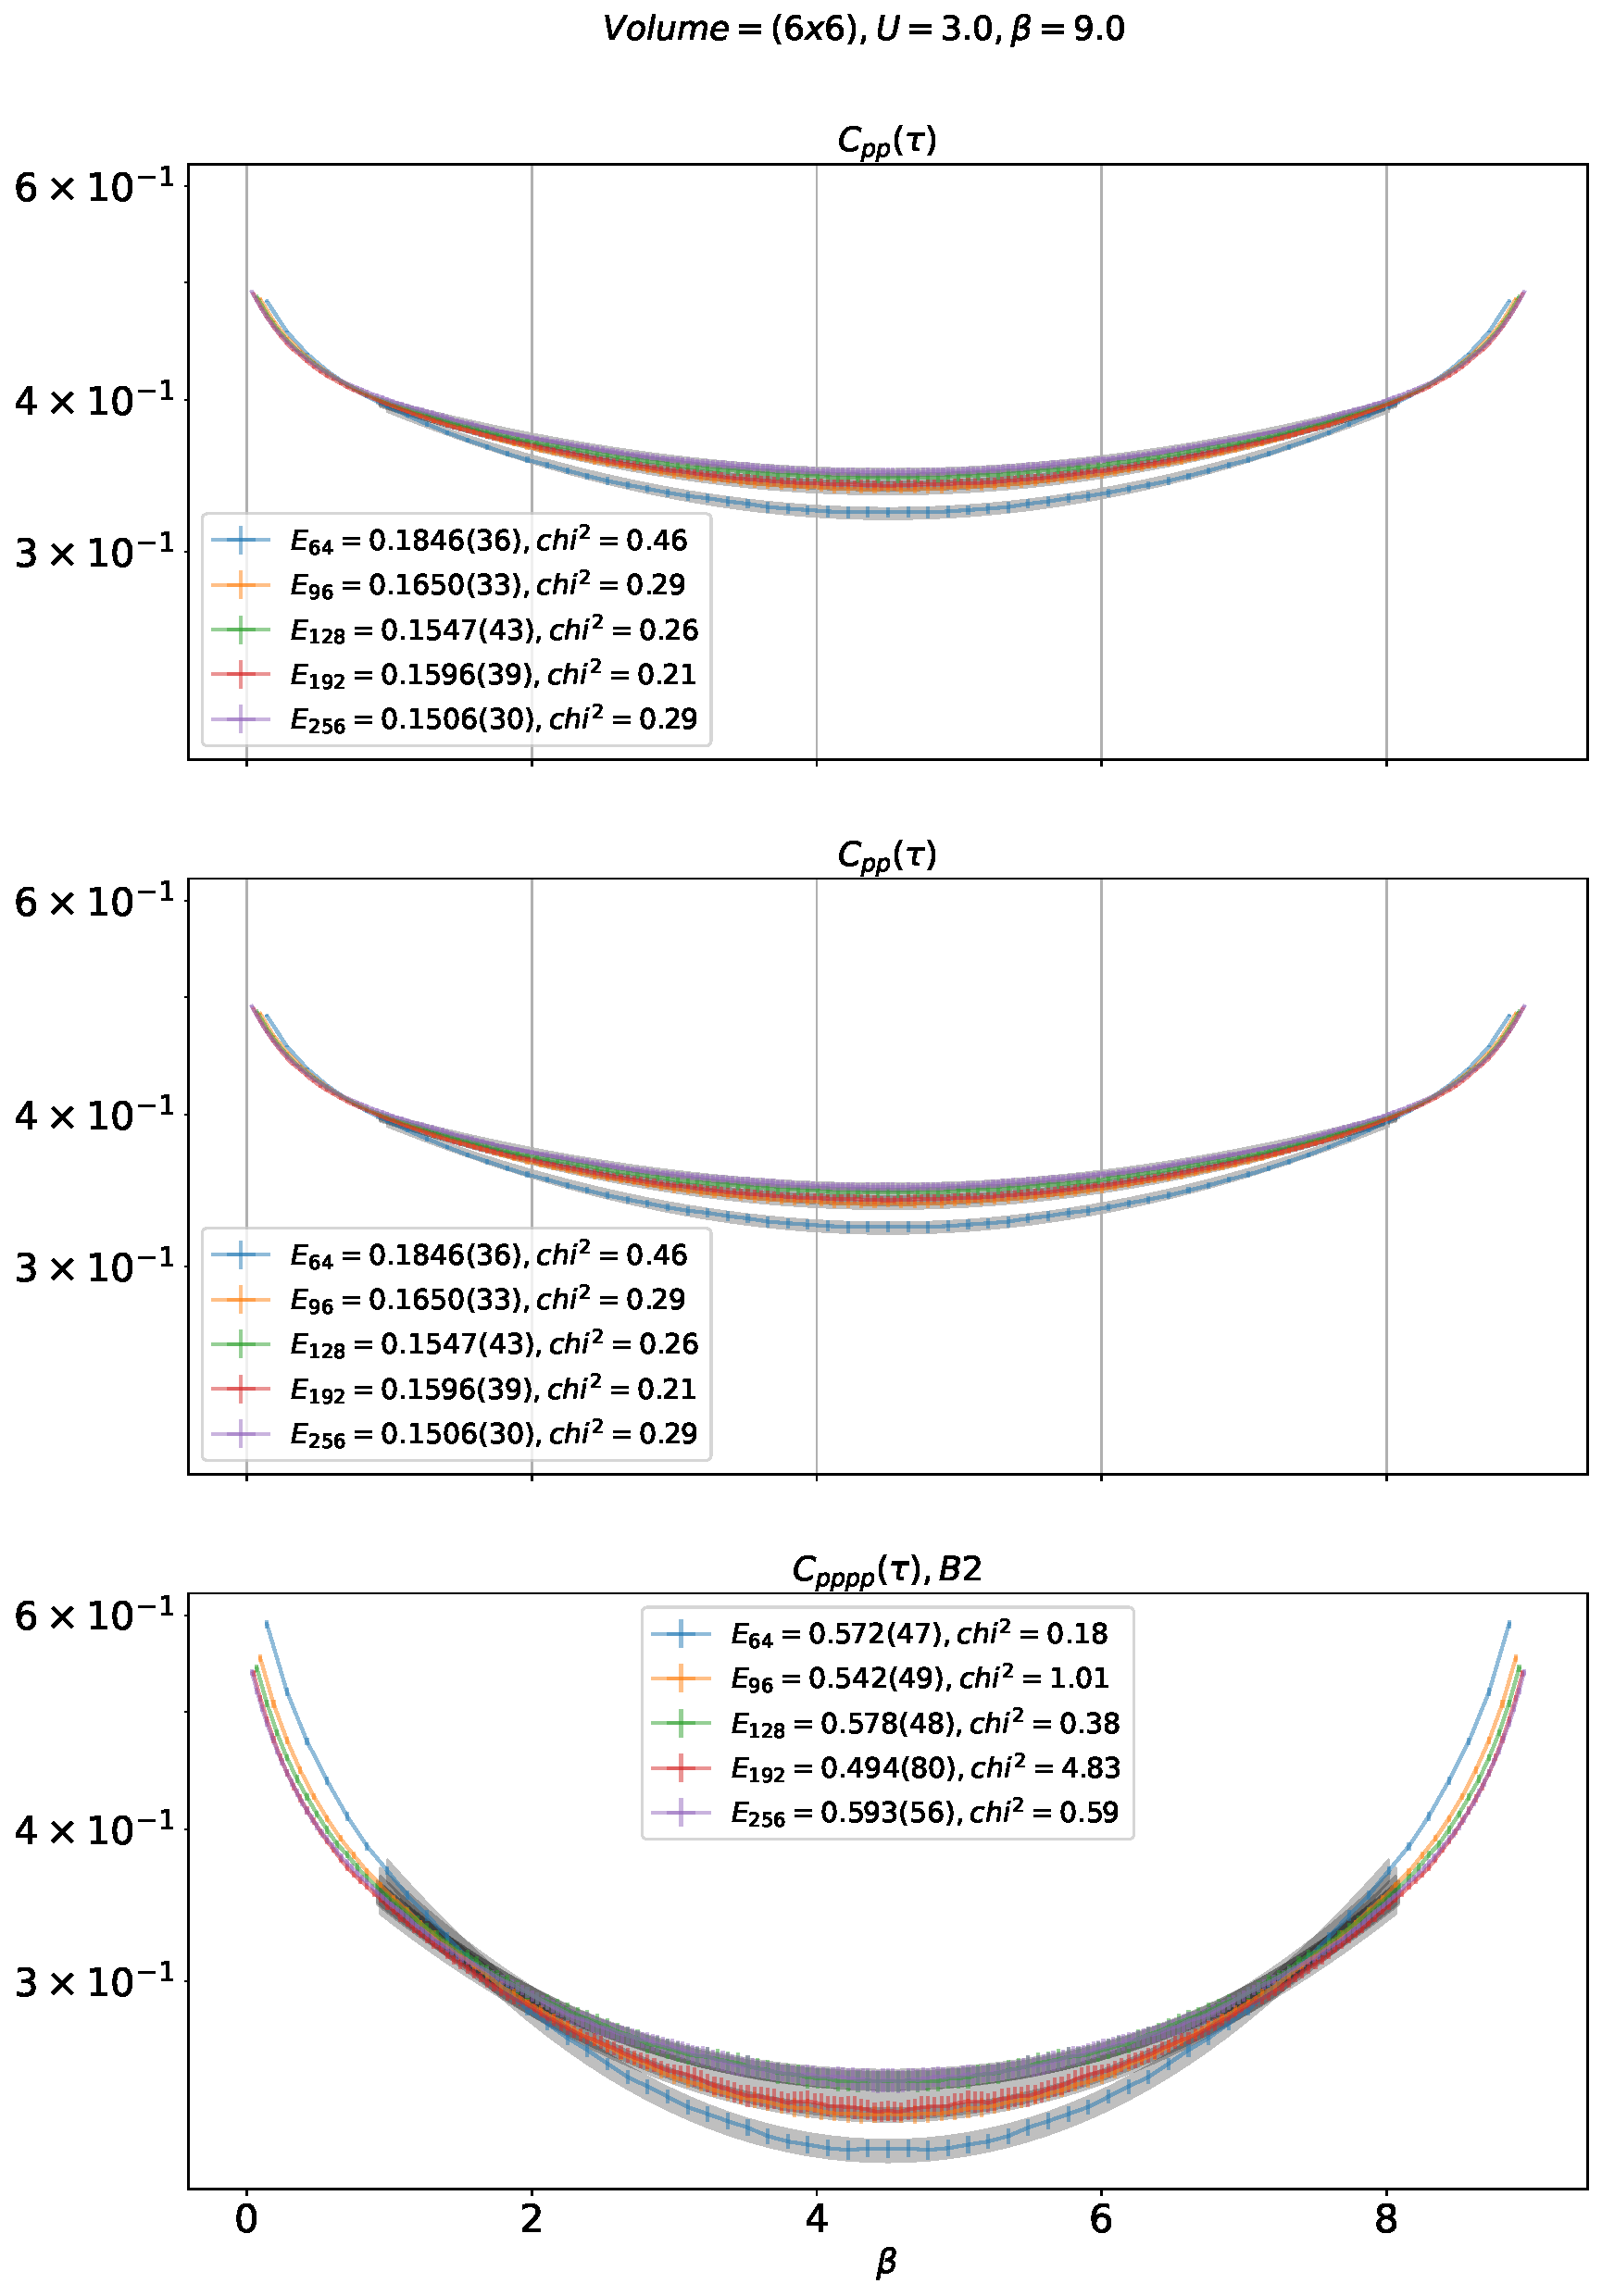
\includegraphics[width=\linewidth]{pppp-0-B2_6x6_U3.0_B9.0.pdf}
  \end{subfigure}
  \begin{subfigure}{.5\textwidth}
      \centering
      \includegraphics[width=\linewidth]{pppp-0-A1_6x6_U3.0_B9.0_cont.pdf}
  \end{subfigure}
  \begin{subfigure}{.5\textwidth}
      \centering
      \includegraphics[width=\linewidth]{pppp-0-B2_6x6_U3.0_B9.0_cont.pdf}
  \end{subfigure}
  \caption{Binding energy extraction of the particle-particle pair at both irreducible representations, where we fit one- and two-body correlators for every $N_t$. This is followed by fitting a linear and a quadratic functions to the $\Delta E_{N_t}$ in order to extrapolate to the continuum limit ($N_t\to\infty$).}
  \label{fig:fig13}
\end{figure}

\begin{figure}
  \begin{subfigure}{.5\textwidth}
    \centering
    \includegraphics[width=\linewidth]{pppp-0-A1_6x6_U3.0_B24.0.pdf}
  \end{subfigure}%
  \begin{subfigure}{.5\textwidth}
    \centering
    \includegraphics[width=\linewidth]{pppp-0-B2_6x6_U3.0_B24.0.pdf}
  \end{subfigure}
  \begin{subfigure}{.5\textwidth}
      \centering
      \includegraphics[width=\linewidth]{pppp-0-A1_6x6_U3.0_B24.0_cont.pdf}
  \end{subfigure}
  \begin{subfigure}{.5\textwidth}
      \centering
      \includegraphics[width=\linewidth]{pppp-0-B2_6x6_U3.0_B24.0_cont.pdf}
  \end{subfigure}
  \caption{Binding energy extraction of the particle-particle pair at both irreducible representations, where we fit one- and two-body correlators for every $N_t$. This is followed by fitting a linear and a quadratic functions to the $\Delta E_{N_t}$ in order to extrapolate to the continuum limit ($N_t\to\infty$).}
  \label{fig:fig14}
\end{figure}

\begin{figure}
  \begin{subfigure}{.5\textwidth}
    \centering
    \includegraphics[width=\linewidth]{phhp-0-A1_6x6_U4.0_B6.0.pdf}
  \end{subfigure}%
  \begin{subfigure}{.5\textwidth}
    \centering
    \includegraphics[width=\linewidth]{phhp-0-B2_6x6_U4.0_B6.0.pdf}
  \end{subfigure}
  \begin{subfigure}{.5\textwidth}
      \centering
      \includegraphics[width=\linewidth]{phhp-0-A1_6x6_U4.0_B6.0_cont.pdf}
  \end{subfigure}
  \begin{subfigure}{.5\textwidth}
      \centering
      \includegraphics[width=\linewidth]{phhp-0-B2_6x6_U4.0_B6.0_cont.pdf}
  \end{subfigure}
  \caption{Binding energy extraction of the particle-hole pair at both irreducible representations, where we fit one- and two-body correlators for every $N_t$. This is followed by fitting a linear and a quadratic functions to the $\Delta E_{N_t}$ in order to extrapolate to the continuum limit ($N_t\to\infty$).}
  \label{fig:fig15}
\end{figure}

\begin{figure}
  \begin{subfigure}{.5\textwidth}
    \centering
    \includegraphics[width=\linewidth]{phhp-0-A1_6x6_U4.0_B9.0.pdf}
  \end{subfigure}%
  \begin{subfigure}{.5\textwidth}
    \centering
    \includegraphics[width=\linewidth]{phhp-0-B2_6x6_U4.0_B9.0.pdf}
  \end{subfigure}
  \begin{subfigure}{.5\textwidth}
      \centering
      \includegraphics[width=\linewidth]{phhp-0-A1_6x6_U4.0_B9.0_cont.pdf}
  \end{subfigure}
  \begin{subfigure}{.5\textwidth}
      \centering
      \includegraphics[width=\linewidth]{phhp-0-B2_6x6_U4.0_B9.0_cont.pdf}
  \end{subfigure}
  \caption{Binding energy extraction of the particle-hole pair at both irreducible representations, where we fit one- and two-body correlators for every $N_t$. This is followed by fitting a linear and a quadratic functions to the $\Delta E_{N_t}$ in order to extrapolate to the continuum limit ($N_t\to\infty$).}
  \label{fig:fig16}
\end{figure}

\begin{figure}
  \begin{subfigure}{.5\textwidth}
    \centering
    \includegraphics[width=\linewidth]{phhp-0-A1_6x6_U4.0_B24.0.pdf}
  \end{subfigure}%
  \begin{subfigure}{.5\textwidth}
    \centering
    \includegraphics[width=\linewidth]{phhp-0-B2_6x6_U4.0_B24.0.pdf}
  \end{subfigure}
  \begin{subfigure}{.5\textwidth}
      \centering
      \includegraphics[width=\linewidth]{phhp-0-A1_6x6_U4.0_B24.0_cont.pdf}
  \end{subfigure}
  \begin{subfigure}{.5\textwidth}
      \centering
      \includegraphics[width=\linewidth]{phhp-0-B2_6x6_U4.0_B24.0_cont.pdf}
  \end{subfigure}
  \caption{Binding energy extraction of the particle-hole pair at both irreducible representations, where we fit one- and two-body correlators for every $N_t$. This is followed by fitting a linear and a quadratic functions to the $\Delta E_{N_t}$ in order to extrapolate to the continuum limit ($N_t\to\infty$).}
  \label{fig:fig17}
\end{figure}

\begin{figure}
  \begin{subfigure}{.5\textwidth}
    \centering
    \includegraphics[width=\linewidth]{pppp-0-A1_6x6_U4.0_B6.0.pdf}
  \end{subfigure}%
  \begin{subfigure}{.5\textwidth}
    \centering
    \includegraphics[width=\linewidth]{pppp-0-B2_6x6_U4.0_B6.0.pdf}
  \end{subfigure}
  \begin{subfigure}{.5\textwidth}
      \centering
      \includegraphics[width=\linewidth]{pppp-0-A1_6x6_U4.0_B6.0_cont.pdf}
  \end{subfigure}
  \begin{subfigure}{.5\textwidth}
      \centering
      \includegraphics[width=\linewidth]{pppp-0-B2_6x6_U4.0_B6.0_cont.pdf}
  \end{subfigure}
  \caption{Binding energy extraction of the particle-particle pair at both irreducible representations, where we fit one- and two-body correlators for every $N_t$. This is followed by fitting a linear and a quadratic functions to the $\Delta E_{N_t}$ in order to extrapolate to the continuum limit ($N_t\to\infty$).}
  \label{fig:fig18}
\end{figure}

\begin{figure}
  \begin{subfigure}{.5\textwidth}
    \centering
    \includegraphics[width=\linewidth]{pppp-0-A1_6x6_U4.0_B9.0.pdf}
  \end{subfigure}%
  \begin{subfigure}{.5\textwidth}
    \centering
    \includegraphics[width=\linewidth]{pppp-0-B2_6x6_U4.0_B9.0.pdf}
  \end{subfigure}
  \begin{subfigure}{.5\textwidth}
      \centering
      \includegraphics[width=\linewidth]{pppp-0-A1_6x6_U4.0_B9.0_cont.pdf}
  \end{subfigure}
  \begin{subfigure}{.5\textwidth}
      \centering
      \includegraphics[width=\linewidth]{pppp-0-B2_6x6_U4.0_B9.0_cont.pdf}
  \end{subfigure}
  \caption{Binding energy extraction of the particle-particle pair at both irreducible representations, where we fit one- and two-body correlators for every $N_t$. This is followed by fitting a linear and a quadratic functions to the $\Delta E_{N_t}$ in order to extrapolate to the continuum limit ($N_t\to\infty$).}
  \label{fig:fig19}
\end{figure}

\begin{figure}
  \begin{subfigure}{.5\textwidth}
    \centering
    \includegraphics[width=\linewidth]{pppp-0-A1_6x6_U4.0_B24.0.pdf}
  \end{subfigure}%
  \begin{subfigure}{.5\textwidth}
    \centering
    \includegraphics[width=\linewidth]{pppp-0-B2_6x6_U4.0_B24.0.pdf}
  \end{subfigure}
  \begin{subfigure}{.5\textwidth}
      \centering
      \includegraphics[width=\linewidth]{pppp-0-A1_6x6_U4.0_B24.0_cont.pdf}
  \end{subfigure}
  \begin{subfigure}{.5\textwidth}
      \centering
      \includegraphics[width=\linewidth]{pppp-0-B2_6x6_U4.0_B24.0_cont.pdf}
  \end{subfigure}
  \caption{Binding energy extraction of the particle-particle pair at both irreducible representations, where we fit one- and two-body correlators for every $N_t$. This is followed by fitting a linear and a quadratic functions to the $\Delta E_{N_t}$ in order to extrapolate to the continuum limit ($N_t\to\infty$).}
  \label{fig:fig20}
\end{figure}

%The \LaTeX\ WikiBook~\cite{latexwiki} is a useful source of information on \LaTeX.
